\documentclass[12pt,oneside]{book}

% \usepackage{natbib}
\usepackage[
    natbib=true,
    style=numeric,
    sorting=none]{biblatex}
\addbibresource{references.bib}

% packages
\usepackage{xspace}
\usepackage{textcase}
\usepackage{dcolumn}
\usepackage{longtable}
\usepackage[version=4]{mhchem}
\usepackage{hyperref}
\usepackage{cleveref}
\usepackage{multirow}
\usepackage{multicol}
\usepackage{wasysym}
\usepackage{graphics}
\usepackage{graphicx}
\usepackage{amsmath}
\usepackage{amsthm}
\usepackage{amssymb}
\usepackage{footnote}
\usepackage{layout}
\usepackage[utf8]{inputenc}
\usepackage{siunitx}
\usepackage{mathtools}
\usepackage{lineno}
\usepackage{ragged2e}
\usepackage{xcolor,fancybox}
\usepackage{listings}
\usepackage{gensymb}
\usepackage{booktabs}
\usepackage{subcaption}

\usepackage[
disable
]{endfloat}

% define the margins of the document
\usepackage{geometry}
\geometry{
    left = 1.5cm,
    right = 1.5cm,
    top = 2cm,
    bottom = 2cm
}

% create the function for illustrating in-line Python code
\newcommand{\pyobject}[1]{
    \ovalbox{\color{red}{\texttt{#1}}}
    } 

% asterix command ([1] => *)
% \usepackage[symbol]{footmisc}
\renewcommand{\thefootnote}{\fnsymbol{footnote}}

% overbar command
\usepackage{amsfonts}
\newcommand{\overbar}[1]{\mkern 2.5mu\overline{\mkern-2.5mu#1\mkern-2.5mu}\mkern 2.5mu}

%%%%%%%%%%%%%%%%% STYLISTIC HEADINGS %%%%%%%%%%%%%%%%%%%%%%%
\pagestyle{headings}
% Note that the line below could be modified to suit a
% particular system since the "geometry" package behaves
% differently in Unix, Windows and Mac, especially for the
% top margins.
% Adjust the parameter "top" (measuring the height of the
% space allocated to a header) and "headsep" (measuring
% the distance from the bottom of the header to the
% first line of text.
% \usepackage[top=1.3in,left=1.5in,bottom=1in,right=1in,headsep=0.5in]{geometry}

\usepackage{setspace}
\onehalfspacing
%\doublespacing

% Headers and footers for thesis
\usepackage{fancyhdr}

\markboth{}{}
\newcommand\startchapter[1]{\chapter{#1}\thispagestyle{myheadings}}
\newcommand\startappendix[1]{\chapter{#1}\thispagestyle{myheadings}}
\newcommand\startfirstchapter[1]{\chapter{#1}}

% Manual addition of section to Table of Contents
\newcommand\TOCadd[1]{\newpage\phantomsection\addcontentsline{toc}{chapter}{#1}}

% Float Customization
\renewcommand{\floatpagefraction}{0.01}

% Customization of Tables of Contents and List of Figures/Tables
\usepackage{tocloft}
\renewcommand\cfttabpresnum{Table\ }
\renewcommand\cfttabnumwidth{0.75in}
\renewcommand\cftfigpresnum{Figure\ }
\renewcommand\cftfignumwidth{0.80in}
\newcommand{\HRule}{\rule{\linewidth}{0.5mm}}

%%%%%%%%%%%%%%%%%%%% DEFINE COMMANDS %%%%%%%%%%%%%%%%%%%%%%%%
\newcommand{\beginsupplement}{%
        \setcounter{table}{0}
        \renewcommand{\thetable}{S\arabic{table}}%
        \setcounter{figure}{0}
        \renewcommand{\thefigure}{S\arabic{figure}}%
        \setcounter{equation}{0}
        \renewcommand{\theequation}{S\arabic{equation}}%
     }
% \newcommand{\endsupplement}{%
%         \setcounter{table}{0}
%         \renewcommand{\thetable}{\arabic{table}}%
%         \setcounter{figure}{0}
%         \renewcommand{\thefigure}{\arabic{figure}}%
%         \setcounter{equation}{0}
%         \renewcommand{\theequation}{\arabic{equation}}%
%      }


\newenvironment{supplementary}{
    \setcounter{table}{0}       
    \renewcommand{\thetable}{S\arabic{table}}        
    \setcounter{figure}{0}         
    \renewcommand{\thefigure}{S\arabic{figure}} 				 
    \setcounter{equation}{0}         
    \renewcommand{\theequation}{S\arabic{equation}}
    } 

\renewcommand{\thefootnote}{\roman{footnote}}


\begin{document}

% Front Matter
\input frontmatter/fm

\newpage

% chapters
\linenumbers
\newpage
\startfirstchapter{Introduction}

\section{Motivation}
This Thesis sought to develop practical tools that can cultivate a sustainable society. The two specific problems that are addressed herein are 1) water insecurity and 2) antimicrobial resistance (AMR), which converge in desalination technologies. The research of this Thesis produced application programming interfaces (APIs) as computational tools that can facilitate technological development towards resolving these growing problems in society.

\section{Water security}
Fresh water resources are diminishing \cite{Laghari2013MeltingUncertainty,Rasul2008GlobalRanges}, despite that water is one of the most abundant chemicals on Earth \cite{Shiklomanov1993WorldResources}. This is a consequence of global warming \cite{Hansen2006GlobalChange,IPCC2018Global1.5C} and climate change \cite{Thomas2004ExtinctionChange} that disrupt the water cycle, and pollution \cite{Pappas2017EnergySuperpower,Zhao2016DecouplingInvestment,Moller2010DistributionWatershed} and over-consumption \cite{Bongaarts2009HumanTransition,Meyer1992HumanChange} that contaminate and deplete water reserves, respectively. One of the many consequences of less available freshwater is that billions of people \cite{Unicef2017ThirstingClimate}, who disproportionately reside in developing nations, experience water insecurity each year \cite{Hoekstra2012GlobalAvailability}. This disparity in access to potable water is recognized as a top global priority in the 6th UN Sustainable Development Goal \cite{Jones2018TheOutlook}. 

Desalination is a promising technology that may resolve water insecurities. Desalination enables municipalities to generate potable freshwater from diverse feed sources, especially oceans \cite{2018DepartmentWater,Service2006DesalinationUp} that are both within $100 km$ for $\approx \frac{1}{2}$ of the human population \cite{Amy2017Membrane-basedProspects} and are practically inexhaustible relative to the magnitude of human consumption. The most common desalination method is the spiral-wound reverse osmosis (RO) design, since it optimizes the filtration surface area  per unit volume. A cross-sectional schema of RO is represented in Figure \ref{membrane_schema}. These membranes, when operational, selectively permit the diffusion of water across the membrane while impurities are retained in the feed channel. The accumulation of ionic, chemical, and microbial impurities in the feed channel during desalination compromises filtration via membrane fouling \cite{Goosen2004FoulingReview}, of which scaling -- mineral precipitation and deposition upon the membrane surface \cite{Warsinger2015ScalingReview,Khan2013SourceSea,Tang2014FoulingPlant,Shmulevsky2017AnalysisMembranes} -- and biofouling \cite{Characklis1983BiofilmsFouling,Flemming1997ReverseBiofouling,Ridgway1991BiofoulingMembranes,Ivnitsky2005CharacterizationTreatment,Herzberg2007BiofoulingPressure,Schneider2005DynamicsBiofouling,Flemming1997BiofoulingProcesses,Cantor1969BiologicalMembranes,Murphy2001MicrobiologicalMembranes,Chen2004CommunityApproach} -- microbial colonization of the polymeric filtration membrane \cite{Garcia-Trinanes2021InvestigatingDevice,Suwarno2014BiofoulingDevelopment} -- are the primary types.  

\begin{figure}
    \centering
    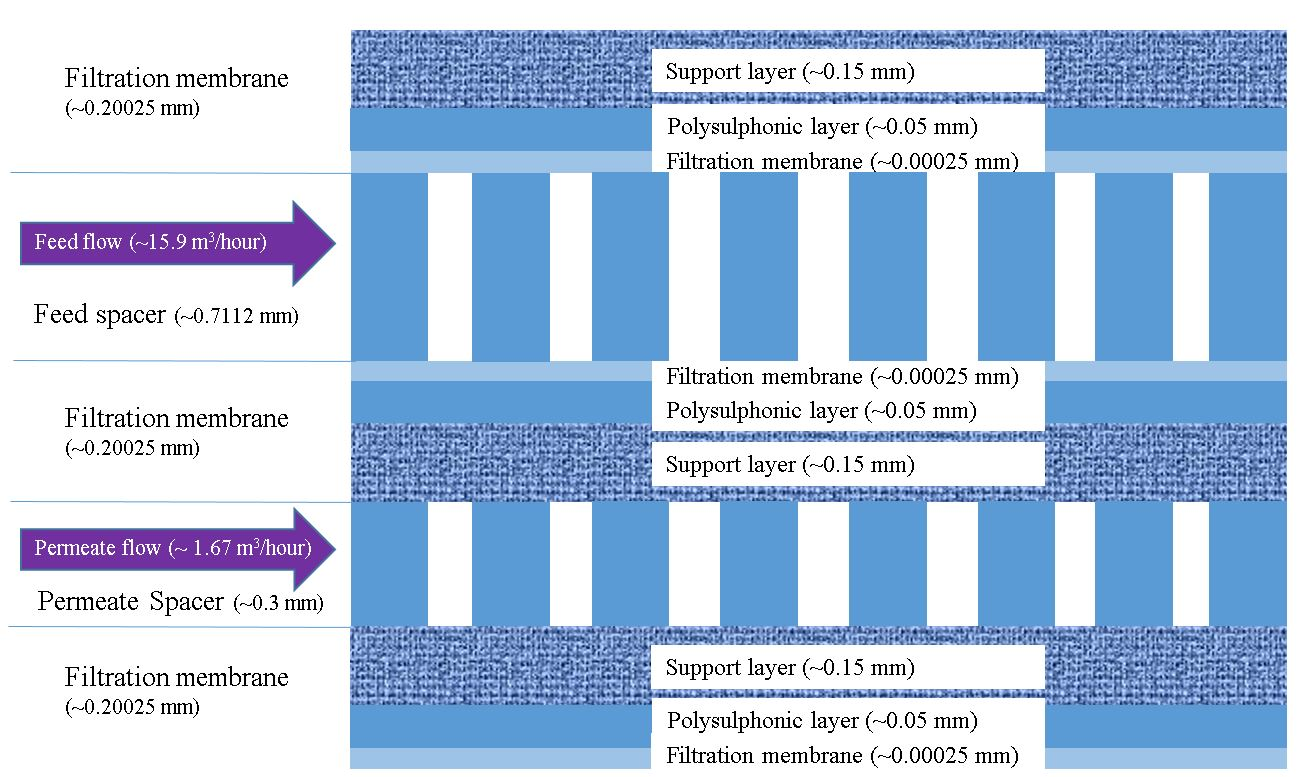
\includegraphics[width = \textwidth]{images/Introduction/membrane_schema.jpg}
    \caption{
        A cross-section of the RO polyamide filtration membrane \cite{Strubbe2018CalibrationFull-Scale}. The quantitative specifications are representative of the default values for our RO model, which are primarily based upon the DOW FILMTEC BW30-400 module.
    }
    \label{membrane_schema}
\end{figure}

\subsection{Scaling}
Scaling in Figure \ref{desalination_schema} is a geochemical phenomena that can occlude and tear the filtration membrane. The geochemical equilibria that result in scaling are difficult to experimentally study; hence, computational software that predict scaling have been developed \cite{Strubbe2018CalibrationFull-Scale}. These software, however, are expensive and/or not accessible via an API, which limits its accessibility and its ability to guide investigators through experimental design. We therefore developed a one-dimensional reactive transport model of desalination, which is sufficiently simple to be numerically encoded in PHREEQC. This PHREEQC expression of our model is the basis of our software, ROSSpy (Reverse Osmosis Scaling Software in Python), which is an intuitive and open-source API that meets identified needs of the RO community to predict brine and scaling from desalination systems. This project is detailed with validation and use cases in Chapter 2.

\begin{figure}
    \centering
    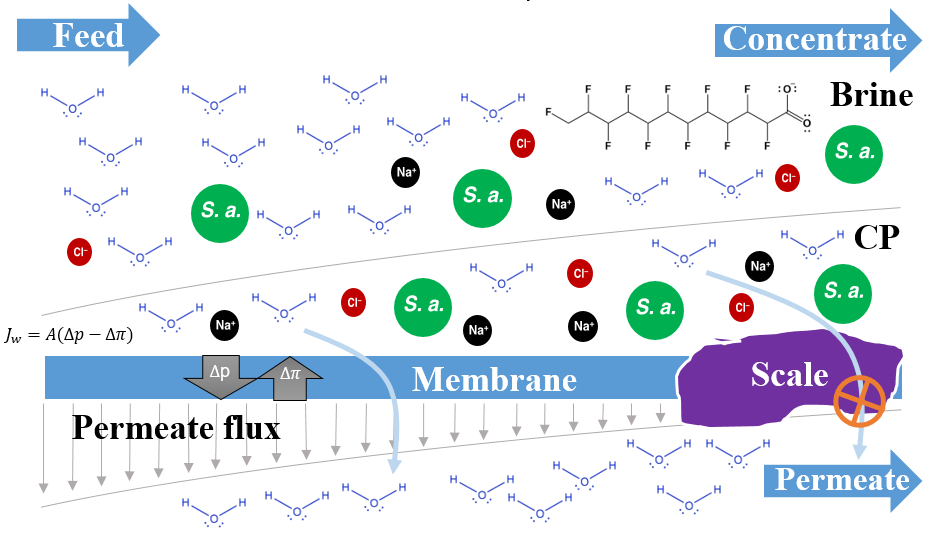
\includegraphics[width = \textwidth]{images/Introduction/desalination_schema_3.PNG}
    \caption{
        A cross-section of RO desalination, which depicts the geochemical environment and the physical hindrance of scaling upon the membrane surface.  Membrane flux decreases over the module distance as a function of the pressure difference between the applied pressure of the feed and the osmotic pressure between the filtered (permeate) water and brine (concentrate) solution.    
    }
    \label{desalination_schema}
\end{figure}

\subsection{Biofouling}
Biofouling is a microbial phenomena, where a surface is colonized and eventually biodegraded. Biocidal treatments can limit biofouling \cite{Kim2009BiocideOverview}, however, these treatments have substantial collateral effects of chemically degrading the filtration membrane \cite{Da-Silva-Correa2022TheReview} and possibly exhibiting off-target effects in the environment \cite{Martins2018Review:Ecosystems,Thomas2001AntifoulingEffects}. The design of benign anti-biofoulants \cite{Buckley2017DesignProducts} is therefore essential to improve the efficacy and sustainability of RO desalination. Innovation here \cite{Winters1983ControlDesalination} can be accelerated by computational tools that allow investigators to predict the effect of different chemical agents and biofilm conditions. We therefore developed the WCMpy (Whole Cell Model in Python) suite of packages to foster the development of such computational tools, which is detailed in Chapter 3. 

% The anti-biofoulant tributyltin oxide, for example, is applied in the coating of boat hulls, yet the chemical gradually leaches into the marine ecosystem where it acts as an immunological toxin to marine animals. An expanding social consciousness of anthropogenic pollution in nature and ultimately human toxification through biomagnification, is encouraging the development of highly specific anti-biofoulants that prevent or treat biofouling without off-target effects.

\section{Antimicrobial resistance}
The treatment of RO biofouling with antibiotics is intertwined with the AMR crisis, where AMR infections are projected to exceed cancer in annual deaths, and globally cost $10^{13}~USD$ in lost economic production, by the mid-21$^{st}$ century \cite{ONeill2014AntimicrobialNations}. The AMR crisis may be mitigated through the use of reactive oxygen species (ROSs), which non-selectively oxidize and kill pathogens while avoiding the mechanisms that result in AMR. ROSs, primarily singlet oxygen ($^1\Delta_g$), can be wielded on demand through photodynamic inactivation (PDI) by simply exposing a photosensitizer (PS) catalyst to incident light of the porper wavelength, which is illustrated in Figure \ref{PDI_workflow}. The innumerable possible combinations of PSs and undesirable microbial targets are unlikely to be completely explored with experiments before mid-century, since resource limitations restrain experimentation. We therefore developed the PDIpy module (Photodynamic Inactivation in Python) to rapidly predict PDI efficacy over a continuum of variable values, which can elucidate effective systems within the space of possible PDI technologies. This project is detailed in Chapter 4. 

\begin{figure}
    \centering
    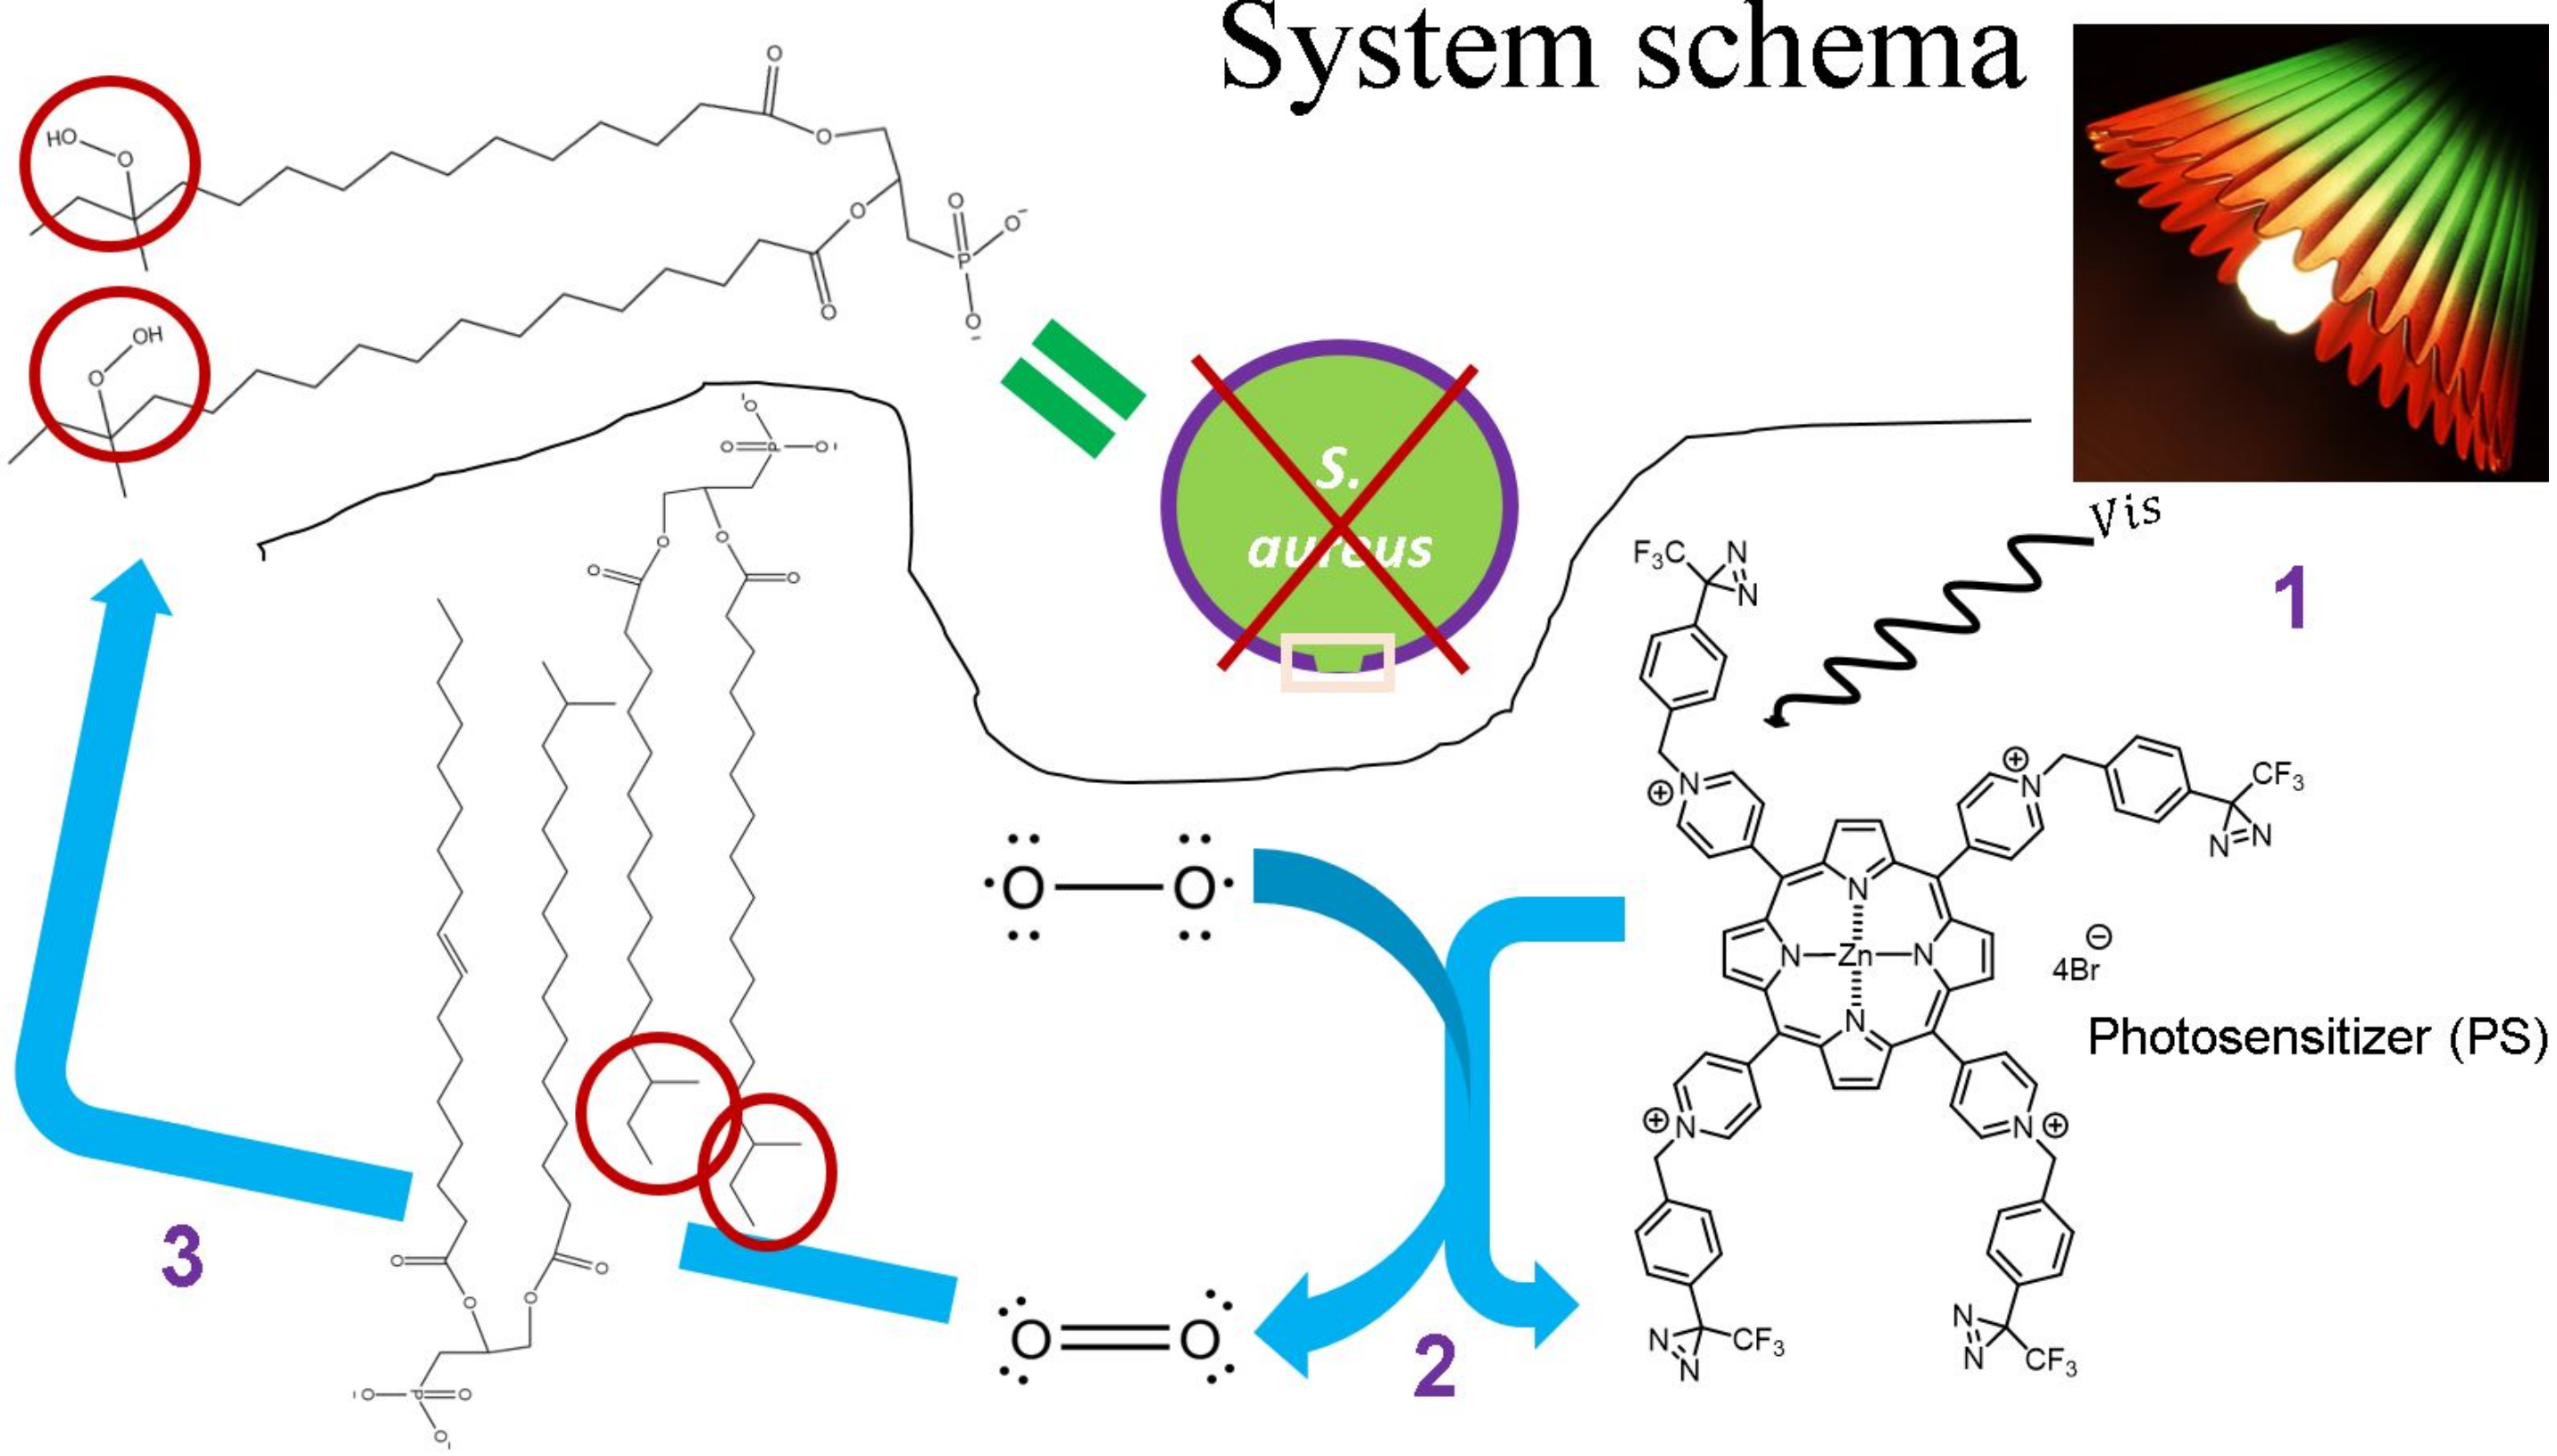
\includegraphics[width = \textwidth]{images/Introduction/PDI_workflow.png}
    \caption{
        A conceptualization of the PDI process: 1) incident light first strikes and excites a PS; 2) the excited PS catalyzes the generation of $\ce{^1O_2}$ from a ground-state oxygen; and 3) the $\ce{^3O_2}$ oxidizes a biological target to the point of cellular death.   
    }
    \label{PDI_workflow}
\end{figure}

\section{Thesis work}
All of the figures and tables in this Thesis are original. The Python modules that have been published in the PyPI (Python Package Index) repository, at least partially for the completion of this Thesis, are listed in Table \ref{downloads} with their respective quantity of PyPI downloads.

\begin{table}
    \centering
    \begin{tabular}{l|c|c|l}
        \textbf{Project} & \textbf{Module} & \textbf{PyPI~downloads} & \textbf{Total}\\
        \toprule
        \multirow{2}{2mm}{ROSSpy} & \href{https://github.com/freiburgermsu/ROSSpy}{ROSSpy} & 10,013 & \multirow{2}{2mm}{21,956}\\
         & \href{https://github.com/freiburgermsu/ChemW}{ChemW} & 11,943 & \\
         \hline
        \multirow{3}{2mm}{WCMpy} & \href{https://github.com/freiburgermsu/Codons}{Codons} & 4,316 & \multirow{3}{2mm}{5,662}\\
         & \href{https://github.com/freiburgermsu/BiGG_SABIO}{BiGG\_SABIO}  & 511 & \\
         & \href{https://github.com/freiburgermsu/dFBApy}{dFBApy} & 835 & \\
         \hline
        PDIpy & \href{https://github.com/freiburgermsu/PDIpy}{PDIpy} & 2,013 & 2,013\\
         \hline
         \textbf{Total} &  &  & \textbf{29,631} \\
         \bottomrule
    \end{tabular}
    \caption{
        The cumulative PyPI downloads according to PePy (\url{https://pepy.tech/}) -- per March 23th, 2022 -- for each of the modules and projects of this Thesis. The GitHub repositories for each module are hyperlinked with the respective module name. 
    }
    \label{downloads}
\end{table}


\section{Future}
The future aspirations for these projects are detailed in Chapter 5. The most notable far-term aspirations include the following: (1) amalgamate the WCMpy suite into a single module that simulates the biochemical effects of an anti-biofilm treatment; and (2) couple the mature module from (1) with the brine predictions from ROSSpy to comprehensively represent the effects of scaling and biofouling, and their interdependence \cite{Radu2014ASystems,Radu2010ModelingPassage}, from RO desalination. This may include the assessment of halophilic bacteria \cite{Bagheri2019ARuber} that could thrive in RO brine.

\newpage
\startchapter{A one-dimensional model of scaling in Reverse Osmosis: ROSSpy}
\label{ROSSpy_chapter}

\section{Introduction}
Desalination technologies, most notably reverse osmosis (RO) \cite{Malaeb2011ReverseReview}, are imperative for meeting the 6th UN Sustainable Development Goal \cite{Jones2018TheOutlook} of universalizing potable freshwater. Arid Middle-Eastern countries, who are both relatively affluent and geographically prone to water scarcity, are embracing RO desalination to satisfy domestic water needs; Israel, for example, supplies $\frac{3}{4}$ of its domestic water from desalination \cite{Shemer2017SustainableImpact} and Saudi Arabia is responsible for $\approx 22\%$ of global water desalination \cite{Council2021WaterPrivatization}. RO is the most economical desalination technology \cite{Karime2008ROPlant,Hafez2003EconomicsStudy}, however, it remains insufficiently efficient and economical for the low-resource communities. RO efficiency can be improved \cite{Elimelech2011TheEnvironment,Semiat2008EnergyProcesses} a) with energy recovery devices \cite{Amy2017Membrane-basedProspects}, that allow RO to approach the thermodynamic limit of desalinating seawater \cite{Zarzo2018DesalinationFuture}, and b) by mitigating membrane fouling such as scaling \cite{Warsinger2015ScalingReview,Khan2013SourceSea,Tang2014FoulingPlant,Shmulevsky2017AnalysisMembranes}, where minerals deposit upon the membrane surface and decrease membrane permeability such that greater applied pressures and energy usage are required to maintain a permeate flux over time. Scaling occurs mechanistically either through homogeneous precipitation from the highly concentrated brine byproduct of RO \cite{VanWagner2009EffectPerformance,Belfer1998SurfaceMembranes} -- which is itself hazardous \cite{Fernandez-torquemada2012DispersionPlants,Clemens1955ToxicityWells,Allen1989ApparatusBrine,Munn1989EffectCrops} but can be processed into useful salts \cite{Allen1954ProcessBrine,Fenton1992DesalinationWells} in zero-liquid waste management systems \cite{Jeppesen2009MetalConcentrate,Mavukkandy2019BrineGeneration} or used in mixing-entropy batteries \cite{Ye2019Charge-FreeMaterials} -- or through heterogeneous deposition upon nucleation sites on the membrane surface \cite{Karabelas2014IncipientChannels,Warsinger2018InorganicOsmosis}. The heterogeneous mechanism specifically occurs in a hyper-concentrated layer adjacent to the membrane called the concentration polarization (CP)   \cite{McCutcheon2006InfluenceOsmosis,Murthy1997EstimationModel,Gruber2011ComputationalSystems,Sablani2001ConcentrationReview,Zydney1997StagnantSystems,Li2016Three-dimensionalChannel}, which is achieved as a consequence of the no-slip boundary condition -- analogous to the capillary effect -- that prevents the CP from mixing with the bulk solution since the velocity gradient of the fluid reaches zero adjacent to the stationary filtration membrane \cite{Rapp2017Fluids}. 

Scaling, unfortunately, is experimentally elusive \cite{Hu2014Real-timeSpectroscopy,Butt1995IdentificationAutopsy,Sheikholeslami2003KineticsM}. Computational programs \cite{Giere2009IsExperimentation,Wijmans1995TheReview} may supplement experimental procedures \cite{Lenhard2007ComputerModeling,Chai2007UltrasoundModules} as a means to investigate scaling and optimize RO efficiency; however, current programs are either unspecific to RO \cite{2018ZeroPHREEQC} or focus upon other aspects of RO: e.g. plant operation \cite{DesalitechROSASoftware,Chee2018PerformanceSoftware,SysCAD2020PHREEQCUnit,Bouchareb2019ExperimentalDesalination}, permeate flux \cite{Xu2012TOUGHREACT.0,Steefel2015ReactiveSimulation}, brine geochemistry \cite{Kundu2018TechnicalTechnology}, or fluid dynamics of the CP \cite{Walker2003AssessmentReaction}. Mathematical programs \cite{Radu2014ASystems,Karabelas2019PredictionSimulator} and some with a user interface \cite{SoftwareReverseOsmosis,Strubbe2018CalibrationFull-Scale} have been developed that simulate RO scaling, however, these lack an application programming interfaces (APIs), which is essential for the broad analyses, over a continuum of variables, that could accelerate geochemical scaling research. 

We therefore developed a unique one-dimensional model that captures both the geochemistry of scaling equilibria and the reactive transport of desalination, in contrast to existing one-dimensional RO models that utilize the steady-state approximation and the solution-diffusion model \cite{Strubbe2018CalibrationFull-Scale}. This one-dimensional RO model -- similar only to the WaterTap model \cite{NAWI2021WaterTap} -- is critically amenable with PHREEQC \cite{Parkhurst2015PhreeqcRM:PHREEQC,Charlton2011ModulesLanguages}, which provides a rigorous and open-source numerical implementation of our model, similar to previous studies of scaling \cite{Mitrouli2016CalciumExperiments,Warsinger2018InorganicOsmosis} and RO \cite{Bein1993OriginBrine,Wilson1993GeochemistryFormations,Casas2012SeawaterElectrodialysis,Yan2017ReverseVelocity}. We exemplify our model through replicating experimental literature and conducting numerous sensitivity analyses across continuums of parameter values. We further developed the only, to our knowledge, open-source API of RO reactive transport (ROSSpy: RO Scaling Software in Python) based upon our model, which fulfills identified needs of a scaling software for RO research \cite{Karabelas2020ScalingTools}, where users can create, execute, process, visualize, and export simulations with predicted scale mass per membrane filtration area ($\frac{g~scale}{filtration~m^2}$) and ionic brine concentrations. Developers are encouraged to contribute to ROSSpy, which we believe is an important stride towards satisfying research needs in scaling and ultimately reducing water insecurity, especially in low-resource contexts. 

\section{Methods}

\subsection{Conceptual}

Our model represents RO desalination as a one-dimensional reactive transport process along the membrane-solution interface. The feed is represented by the single-domain model in Figure S4, where the bulk and CP solutions are aggregated into a single solution, as opposed to the more resolved dual-domain model, where the bulk and CP solutions are distinguished (Figure S5) \cite{Chen2016AssessingModel,Scruggs2019TheInterface,Greskowiak2015AUVI,Mieles2012AnalyticalSystem}. The dual-domain remains elusive within the confines of PHREEQC code (Section 6 of the Supporting Information) and moreover we demonstrate that the single-domain model is sufficient to recapitulate experimental results. Our model represents feed at the RO inlet with the Dirichlet boundary condition \cite{Moes2006ImposingMethod,Bazilevs2007WeakMechanics} -- a mathematical description of constant conditions at a model boundary -- where the influent feed is assumed to be an infinite reservoir and thus its concentration is immutable. Our model represents the RO outlet with the Cauchy boundary condition \cite{Gosses2018ExplicitModels} -- a mathematical description of dynamic conditions at a model boundary -- where the effluent concentrations dynamically depend upon desalination. A glossary of parameters and variables for the equations and calculations are provided in Table S1.


\subsection{Numerical}
The geochemistry and reactive transport components of our RO model are numerically detailed in the following sub-sections. 

\subsubsection{Permeate Flux}
The permeate flux in our model is assumed to be 100\% water, similar to other RO models \cite{Li2012OptimalDesalination}, and it is calculated as the change in moles ($\Delta \Phi_{e}$) of feed solution in any examined cell $e$. Permeate flux is proportional to the difference between feed pressure $P$ and osmotic pressure $\pi$ \cite{VanWagner2009EffectPerformance,Schock1987MassModules,Lonsdale1965TransportMembranes}
\begin{equation} \label{pressure_differential}
    \Delta \Phi_{e} ~ \alpha ~ (P - \pi),
\end{equation} 
however, these pressures are not readily measured or reported; hence, we calculate the permeate flux via two comparable methods that are elaborated in the following sub-sections.

\paragraph{Method 1: Linear permeate flux}
One method assumes that permeate flux decreases linearly along the RO module. This causes the concentration -- which is represented by the concentration factor (CF) \cite{McCaffrey1987TheHalite.,Casas2012SeawaterElectrodialysis,Kartashevsky2015PhosphateEffluents,Yan2017ReverseVelocity,Evangelista1985APlants}
\begin{equation} \label{cf_definition}
    CF = \frac{initial}{final}~,
\end{equation}
as the quotient of initial to final ionic concentrations (influent vs. effluent), solution masses, or permeate moles \cite{Casas2012SeawaterElectrodialysis,Yan2017ReverseVelocity} -- to increase exponentially along the RO module. The negative slope of permeate flux is calculated between the first cell $1$ and the last cell $n$
\begin{equation} \label{flux_slope}
    slope = \frac{(\Delta \Phi_{n}-\Delta \Phi_{1})}{n}~,
\end{equation}
where the simulated membrane-solution interface is discretized into $n$ equal fractions (cells) of the total module length $l_{module}$. The permeate fluxes in these border cells, $\Delta \Phi_{1}$ and $\Delta \Phi_{n}$, are calculated through a system of equations. One of these equations
\begin{equation} \label{average_permeate_flux}
     \overbar{\Delta \Phi}_{e} = \frac{\Delta \Phi_{module}}{n} = \frac{\Delta \Phi_{n} + \Delta \Phi_{1}}{2}
\end{equation}
equates two definitions of the average permeate flux per cell $e$: 1) $\overbar{\Delta \Phi}_{e} = \frac{\Delta \Phi_{module}}{n}$ from the total permeate flux over the module $\Delta \Phi_{module}$, and 2) $\frac{\Delta \Phi_{n} + \Delta \Phi_{1}}{2}$, as the average between the border cells. The other equation is the definition of relative pressure loss over the RO module \cite{Srivathsan2014ReverseUnsteadiness,Gu2020ModelingNetworks} ($HL ; 0\le HL\le 1$) per \cref{pressure_differential},
\begin{equation} \label{head_loss}
     \Delta \Phi_{n}= \Delta \Phi_{1}*(1-HL),
\end{equation}
which is $\approx 10\%$ \cite{Fraidenraich2009ReverseExperiment,Evangelista1985APlants,Dandavati1975HollowSystems}. The substitution of \cref{head_loss} into \cref{average_permeate_flux} -- given $HL$, $\Delta \Phi_{module}$, and $n$ -- permits calculating $\Delta \Phi_{1}$ and  $\Delta \Phi_{n}$, the flux slope of \cref{flux_slope}, and subsequently $\Delta \Phi_{e}$ from a linear expression of permeate flux per module cell
\begin{equation} \label{intermediary_permeate_flux}
    \Delta \Phi_{e} = (slope*e+\Delta \Phi_{1}).
\end{equation}
% Our permeate efficiency parameter ($PE; 0<PE<1$) applies here as means of considering module inefficiencies like preexisting fouling in the RO module that lessen the permeate flux of the system. The $PE$ scalar attenuates the total module permeate flux over the module through reducing \cref{intermediary_permeate_flux}: i.e. $\Delta \Phi_{old~module} = \Delta \Phi_{new~module}*PE$; $PE=0$ leads to $\Delta \Phi_{e}=0 ~\forall~ e$; and $PE=HL=1$ leads to $\overbar{\Delta \Phi}_{e}=\Delta \Phi_{e} ~\forall~ e$.

The calculation sequence for this permeate flux method is summarized:
\begin{enumerate}
    \item Define $HL$, $\Delta \Phi_{module}$, and $n$
    \item Calculate the permeate flux slope [\cref{flux_slope,average_permeate_flux,head_loss}]
    \item Calculate the permeate flux in each cell $e$ [\cref{intermediary_permeate_flux}]
\end{enumerate}


\paragraph{Method 2: Linear Concentration Factor}
The second method of calculating the permeate flux assumes that the CF increases linearly, which causes the permeate flux to decrease non-linearly, along the RO module. The CF slope is calculated analogously to \cref{flux_slope}:
\begin{equation} \label{average_cf_slope}
    slope_{CF} =\frac{CF_{n}-CF_1}{n}.
\end{equation}
The effluent $CF_{n}$ is the average CF of all effluent ion concentrations 
\begin{equation} \label{cf_calculation_output}
    CF_{n}=\frac{\sum_{i=1}^j(C_{i,brine})}{\sum_{i=1}^j(C_{i,feed})},
\end{equation}
where $C_{i,brine}$ is the effluent concentration and $C_{i,feed}$ is the influent concentration of ion $i$, for all $j$ ions. Defining CF from \cref{cf_definition} in terms of moles of feed solution ($\Phi$, which is assumed to be 100\% water) reveals an equation 
\begin{equation} \label{cf_cell_definition}
    CF_e=\frac{\Phi_0}{\Phi_e}=\frac{\Phi_0}{\Phi_0-\Delta \Phi_{(1,e)}}
\end{equation}
that can calculate the moles of feed at the end of an arbitrary cell $e$ ($\Phi_e$), where $\Delta \Phi_{e} = \Phi_0 - \Delta \Phi_{(1,e)}$ and $\Delta \Phi_{(1,e)}$, as the sum of permeate flux that occurred between cell $1$ and the end of cell $e$, is separately the sum
\begin{equation} \label{moles_removed_to_cell}
    \Delta \Phi_{(1,e)}=\Delta \Phi_{e}+\Delta \Phi_{(1,e-1)}
\end{equation}
of permeate flux before the start of cell $e$ ($\Delta \Phi_{(1,e-1)}=\sum_{j=1}^{e-1}(\Delta \Phi_{j})$) and the permeate flux over cell $e$ ($\Delta \Phi_{e}$). The initial moles of feed $\Phi_0$ is calculated
\begin{equation} \label{feed_mass}
    \Phi_0=V_{feed}*MW_{H_2O}*\rho_{H_2O},
\end{equation}
from the volume of the feed channel $V_{feed}$, which is the product of the module length $l_{module}$ and the cross-sectional area of the feed channel $A_{feed}$
\begin{equation} \label{feed_area}
    A_{feed}=(A_{module}-A_{permeate})*\frac{th_{feed}}{th_{unit}}~,
\end{equation}
where $A_{module}$ and $A_{permeate}$ are the cross-sectional areas of the whole module and the permeate tube, respectively, and $th_{feed}$ and $th_{unit}$ are the thicknesses of the feed channel and the repeating membrane unit in Figure S1, respectively. The linear expression for $CF_e$ 
\begin{equation} \label{cf_permeate_flux}
    CF_e=(slope_{CF})*e+CF_{0}~,
\end{equation}
is then substituted into \cref{cf_cell_definition}, with the slope from \cref{average_cf_slope}, to yield an expression for the permeate flux (a negative change in feed moles) at the end of each examined cell $e$
\begin{equation} \label{moles_removal_per_cell} 
    -\Delta \Phi_{(1,e)}=\frac{\Phi_0}{((\frac{CF_{n}-CF_{0}}{n})*e+CF_{0})}-\Phi_0~,
\end{equation}
which can be substituted into \cref{moles_removed_to_cell} with the sum of previous permeate fluxes ($\Delta \Phi_{(1,e-1)}$) to yield the permeate flux over any examined cell $e$ ($\Delta \Phi_{e}$), analogously to \cref{intermediary_permeate_flux}. Note that $\Delta \Phi_{(1,e-1)}=0$ when $e=1$, since there are no previous cells. 

The calculation sequence for this permeate flux method is summarized:
\begin{enumerate}
    \item Define the effluent CF
    \item Calculate the feed capacity of the module [\cref{feed_mass,feed_area}]
    \item Calculate the CF slope [\cref{average_cf_slope}]
    \item Calculate the permeate flux in each cell [\cref{cf_cell_definition,moles_removed_to_cell,cf_permeate_flux,moles_removal_per_cell}]
\end{enumerate}

\paragraph{Comparison of permeate flux methods}
Scaling predictions from these two permeate flux methods are juxtaposed in Figure \ref{permeate_approach}. The most significant difference is observed at the mid-point of the simulated module ($0.47 m$), where the linear CF method predicts $0.99 \frac{gram}{m^2}$ of Gypsum scale while the linear permeate flux method predicts $0.0196 \frac{gram}{m^2}$ of Gypsum scale. The linear CF method subsequently predicts subtly less scale than the linear permeate method. These different distributions are explained by the dependency of scale upon the solution CF -- where the exponential increase in CF through the linear permeate flux method causes initially less, and then eventually more, scaling than the linear CF method -- however, the scale distribution ultimately equates between these two permeate flux methods to 3 significant digits: $38.7 \frac{gram}{m^2}$. These methods are therefore believed to only subtly affect the distribution, and not the total quantity, of scale within a module. Experimental literature is not known that can verify which method better reflects physical systems. 

\subsubsection{Geochemistry}
The geochemistry of RO scaling in our model is predicated upon the kinetic rate laws and thermodynamic equilibria that define each mineral dissolution and precipitation. These chemical processes are encapsulated in the PHREEQC databases that offer different a) geochemical models, b) permissible ranges of conditions, and c) sets of potential minerals to best represent a given system. These databases are complemented with the ChemW Python package that rigorously calculates the molecular mass of each mineral (see the ChemW PyPI documentation) to permit scaling predictions in the conventional units of $\frac{g~scale}{m^2~membrane}$.

\begin{figure}
    \centering
    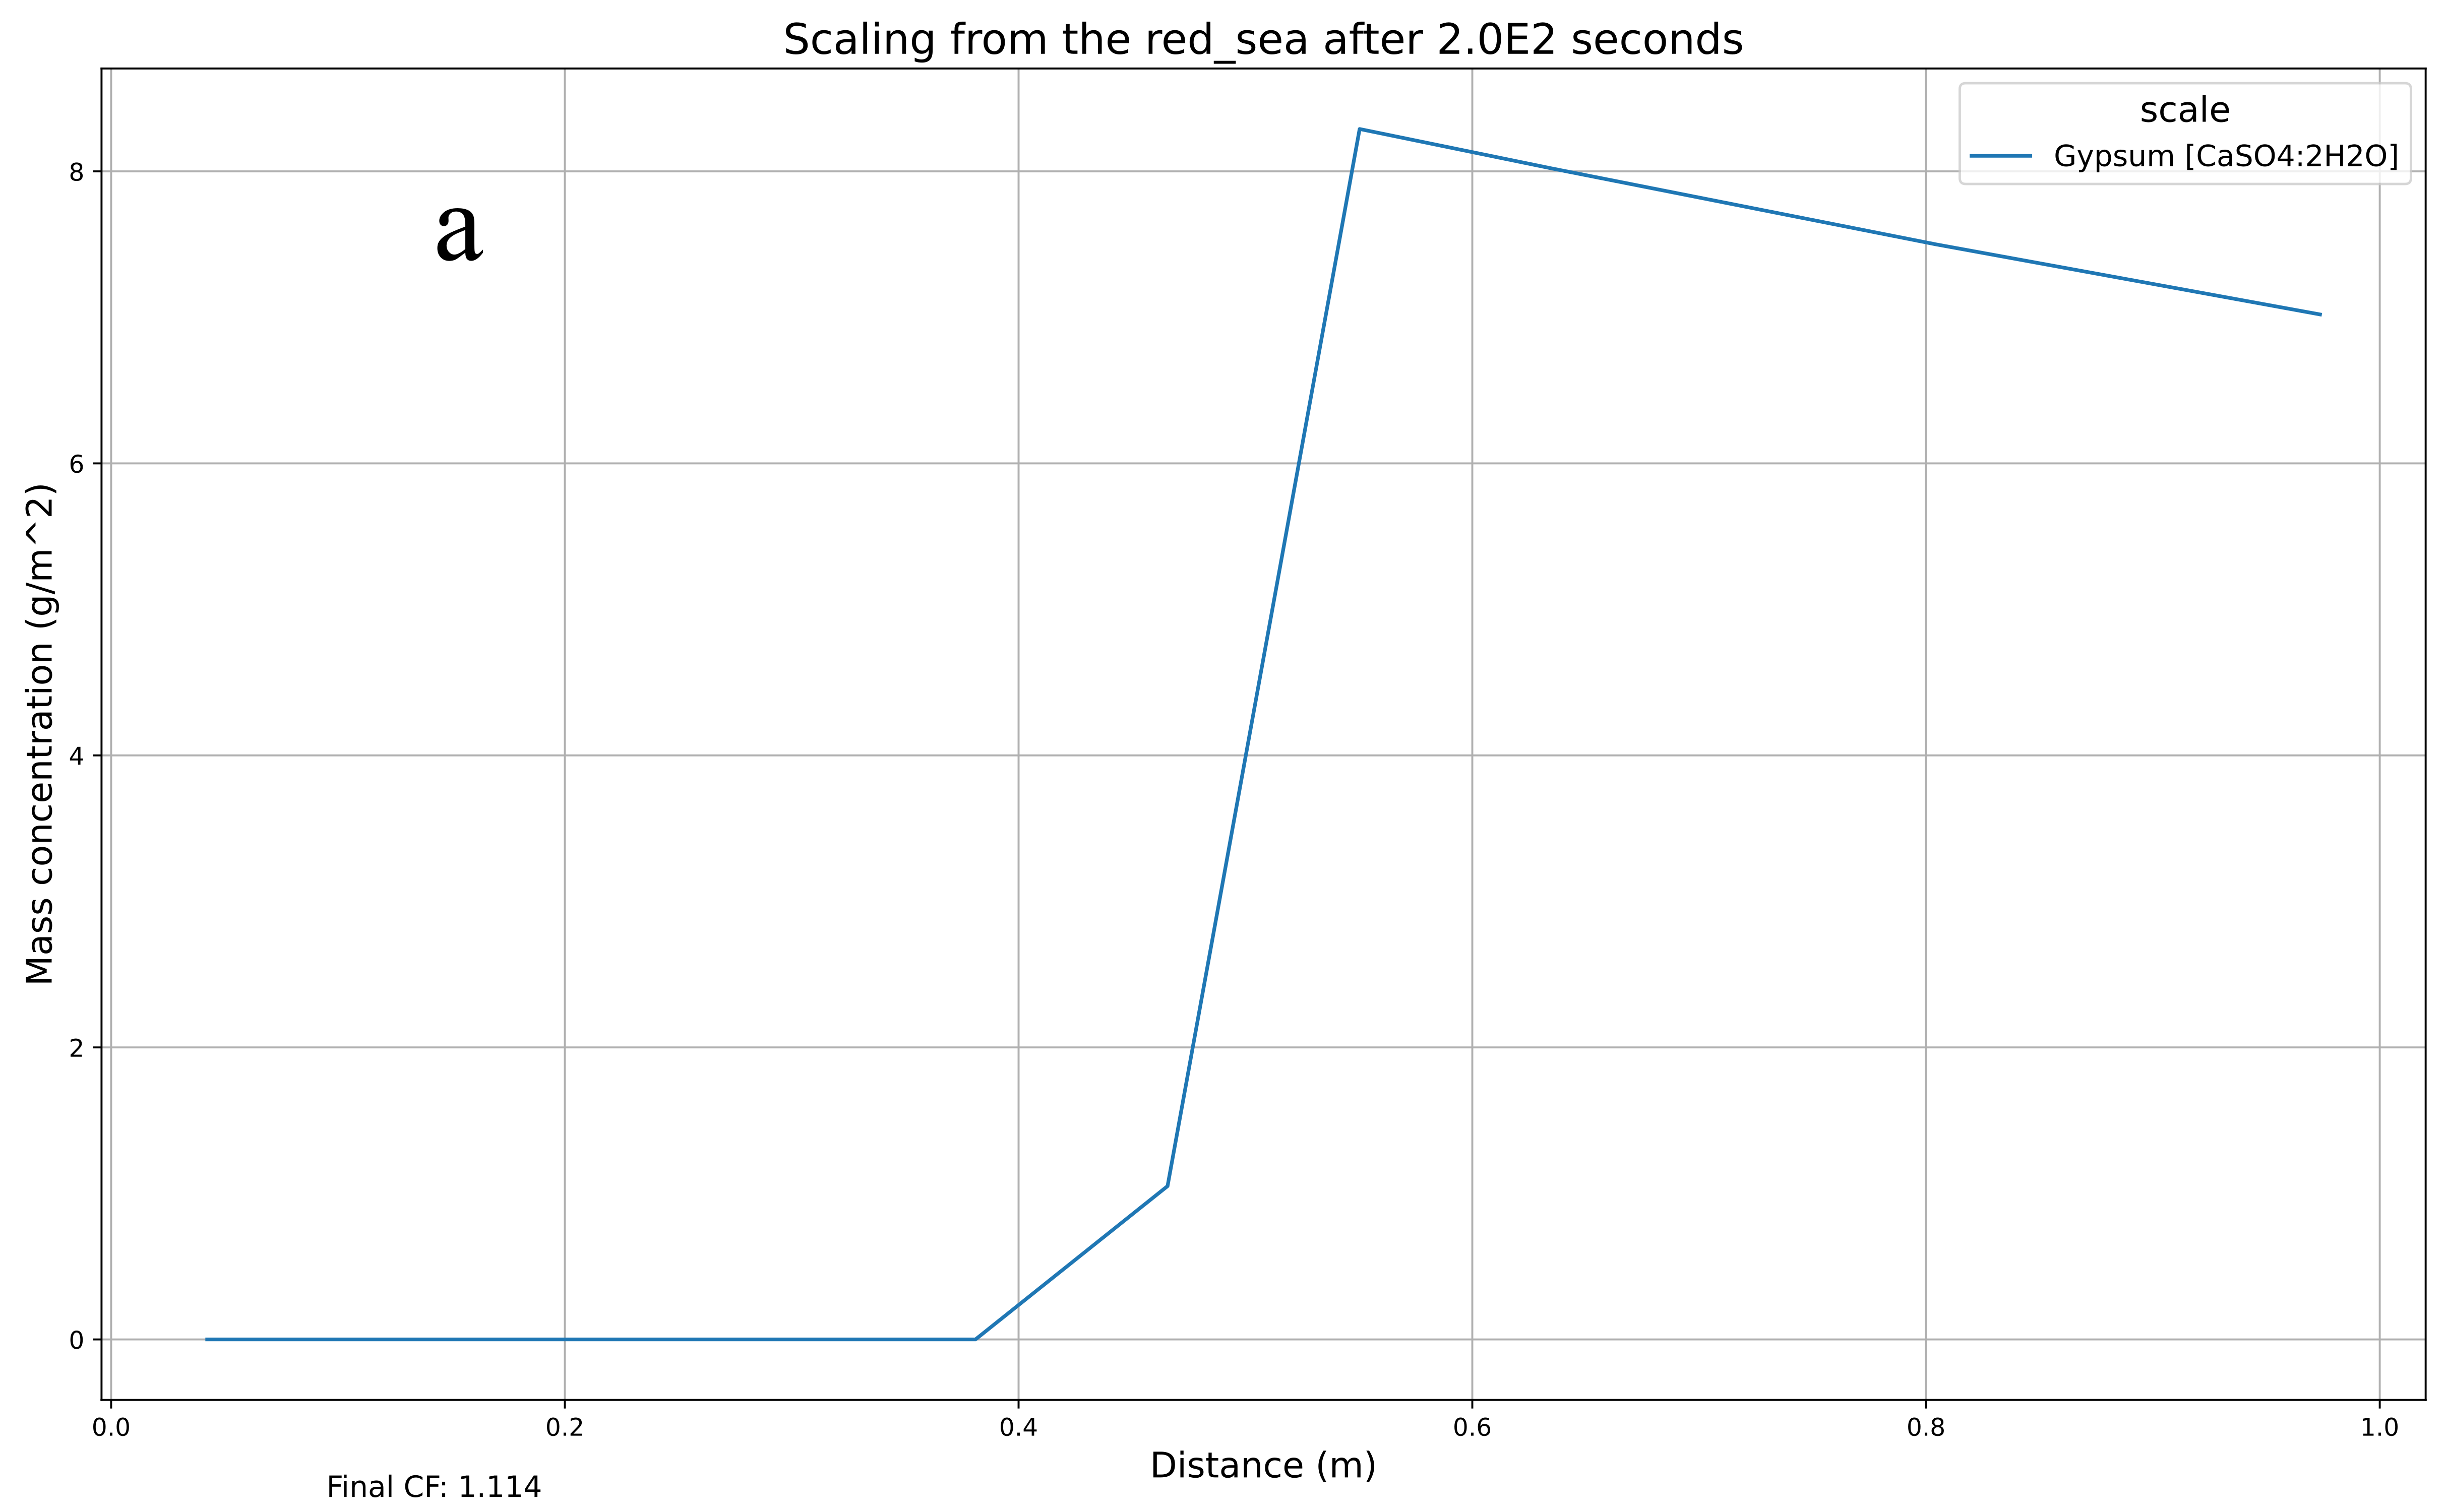
\includegraphics[width=0.9\linewidth]{images/ROSSpy/sensitivity_analyses/permeate_approach/linear_cf.png} \\ \midrule
    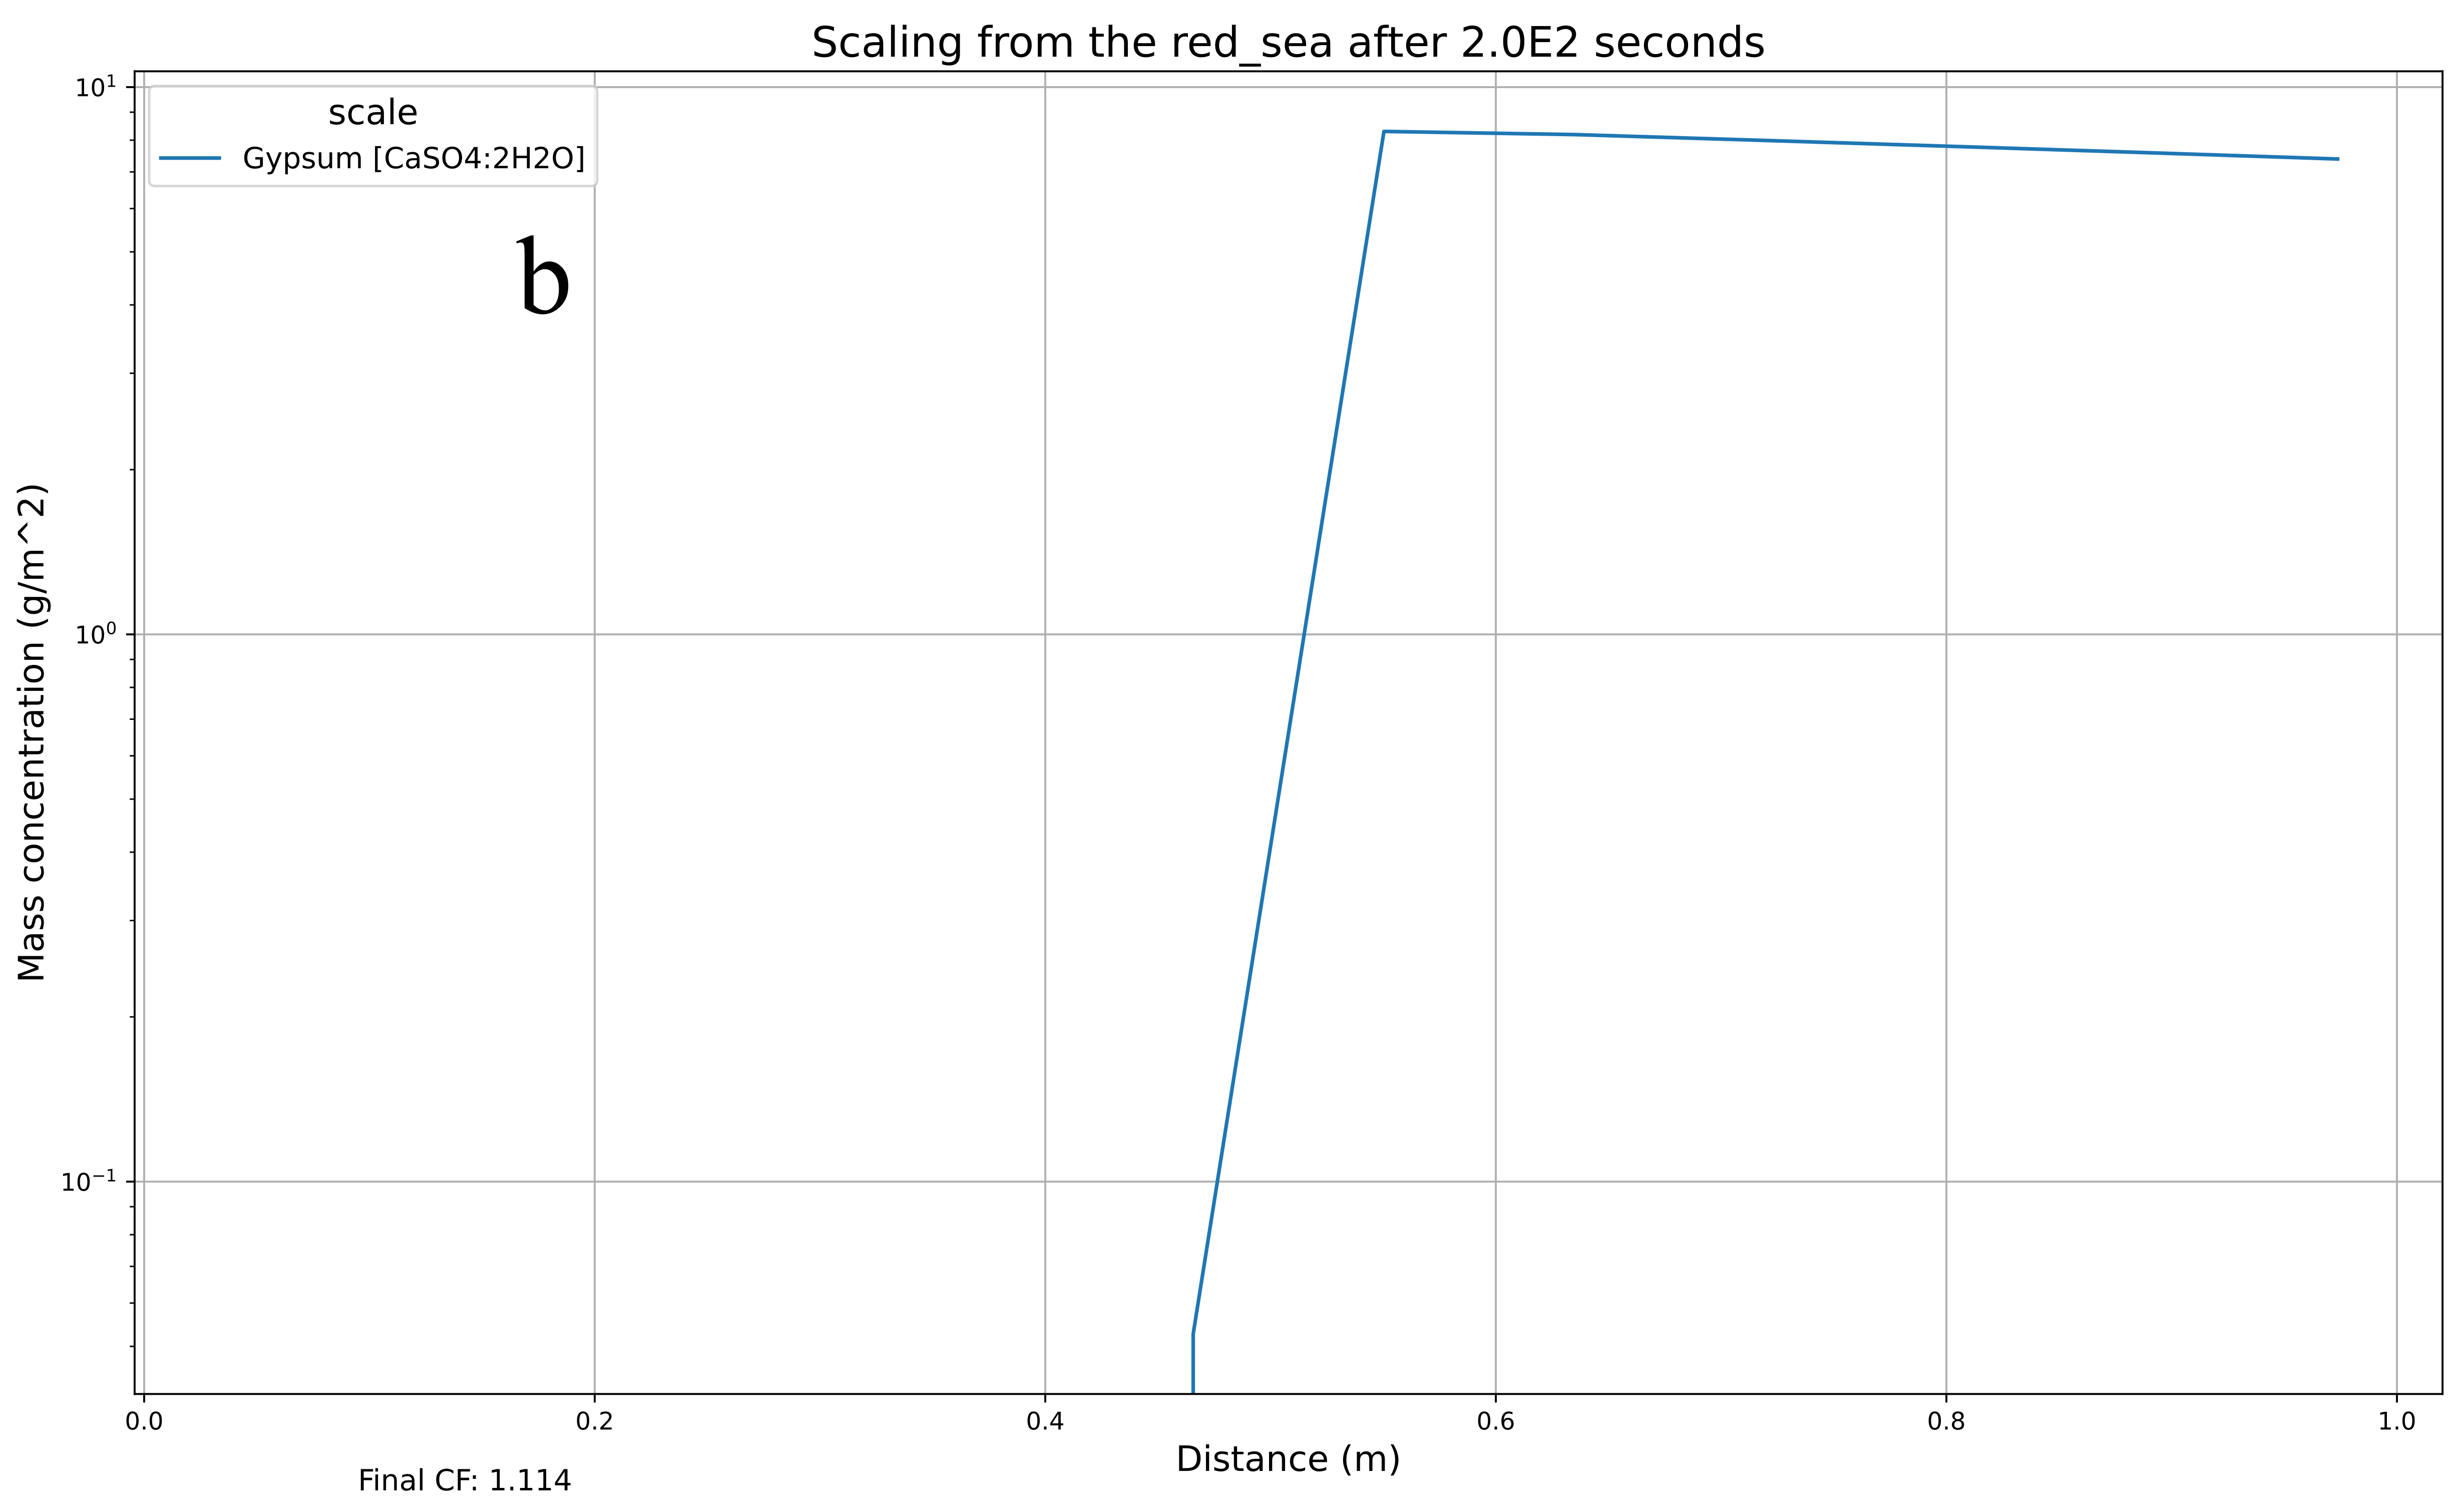
\includegraphics[width=0.9\linewidth]{images/ROSSpy/sensitivity_analyses/permeate_approach/linear_permeate.png} 
    \caption{
        Predicted scaling of the Red Sea at $CF_{effluent}=1.114$ via the a) linear CF and b) linear permeate flux methods. The linear increase in CF of a) slightly homogenizes the distribution of scaling, while the exponential increase in CF of b) skews the distribution of scaling to lesser initially and eventually greater, relative to the linear method of a). These subtle differences in scaling distribution neutralize as the total scaling through both methods are equivalent. 
    }
    \label{permeate_approach}
\end{figure}


\subsubsection{Transport}
The physical transport of feed through the module is simulated in each timestep by 1) migrating the contents of each cell $e$ to the next cell $e+1$; 2) repopulating cell $1$ as new feed solution enters the simulated module; and 3) deleting cell $n$ as brine exits the simulated module. The feed velocity $v_{feed}=\frac{Q_{max~feed}}{A_{feed}}$ is calculated from the maximum feed flowrate $Q_{max~feed}$ ($\frac{m^3}{s}$) and the feed area from \cref{feed_area} of the RO module. Default module parameters in Table S1 are sourced from the DOW FILMTEC BW30-400 RO module, similar to other RO models \cite{Li2012OptimalDesalination}, and supplement user-defined module parameters. The maximum simulation timestep $\Delta t=\frac{l_{cell}}{v_{feed}}$ is calculated according to the Courant Condition \cite{Gnedin2018EnforcingSchemes} ($C_{max}=1 \ge \frac{v_{feed}*t_{max}}{l_{cell}}$) to maintain accurate resolution of the feed flow.

\section{Use cases}
The following sub-sections evince features of our model and its alignment with reported measurements. These studies were conducted through ROSSpy and are available as Python Notebooks in the ROSSpy GitHub repository.

\subsection{CF and Brine formation}
The predicted CF and ionic concentrations of the effluent were verified through comparison with the following three experimental studies, where the reported feed geochemistry and module specifications were parameterized into the model. 

\paragraph{Zaman et al.\cite{Zaman2015DownstreamCompounds}}
This study examines RO brine, from a full-scale water treatment facility in Australia, to understand which minerals are likely to form as scale. The predicted concentrations in Figure \ref{bar_graphs}a were $<6\%-error$ for all but one of the feed ions.

\paragraph{Ahmed et al.\cite{Ahmed2001BrineEmirates}}
This study examines RO brine from 10 small desalination plants in Oman and 8 plants in the United Arab Emirates (UAE) for the purpose of understanding ideal brine disposal methods. We selected the UAE Qidfa I desalination plant from these 18 plants to replicate, since it provided the most comprehensive details. The predicted concentrations in Figure \ref{bar_graphs}b were $<10\%-error$ for all but one of the feed ions. The CF, in the far-right column of Figure \ref{bar_graphs}b, furthermore exhibits a $<1\%-error$, which supports that the reactive transport processes, notably the permeate flux calculations, are accurate.

\paragraph{Hajbi et al.\cite{Hajbi2010ReuseBrine}}
This study  evaluates the recovery of commodity salts from RO brine at a plant in Tunisia. The authors detail specifications of line D -- a polyamide filtration membrane -- in the plant system, in addition to the feed geochemistry, which were all parameterized into our model. The predicted concentrations in Figure \ref{bar_graphs}c were less aligned than the aforementioned two studies, with two ions exceeding $25\%-error$. This is attributed to $40\%$ fewer feed ions being defined by this study, where the incomplete geochemical representation of the feed skews the geochemical calculations of PHREEQC. This is corroborated by the accuracy of the CF prediction in Figure \ref{bar_graphs}c, despite inaccurate concentration predictions, which suggests that the error resides with the geochemical processes and not the reactive transport system. 

\begin{figure}
    \centering
    \begin{tabular}{c|c}
        \multicolumn{2}{c}{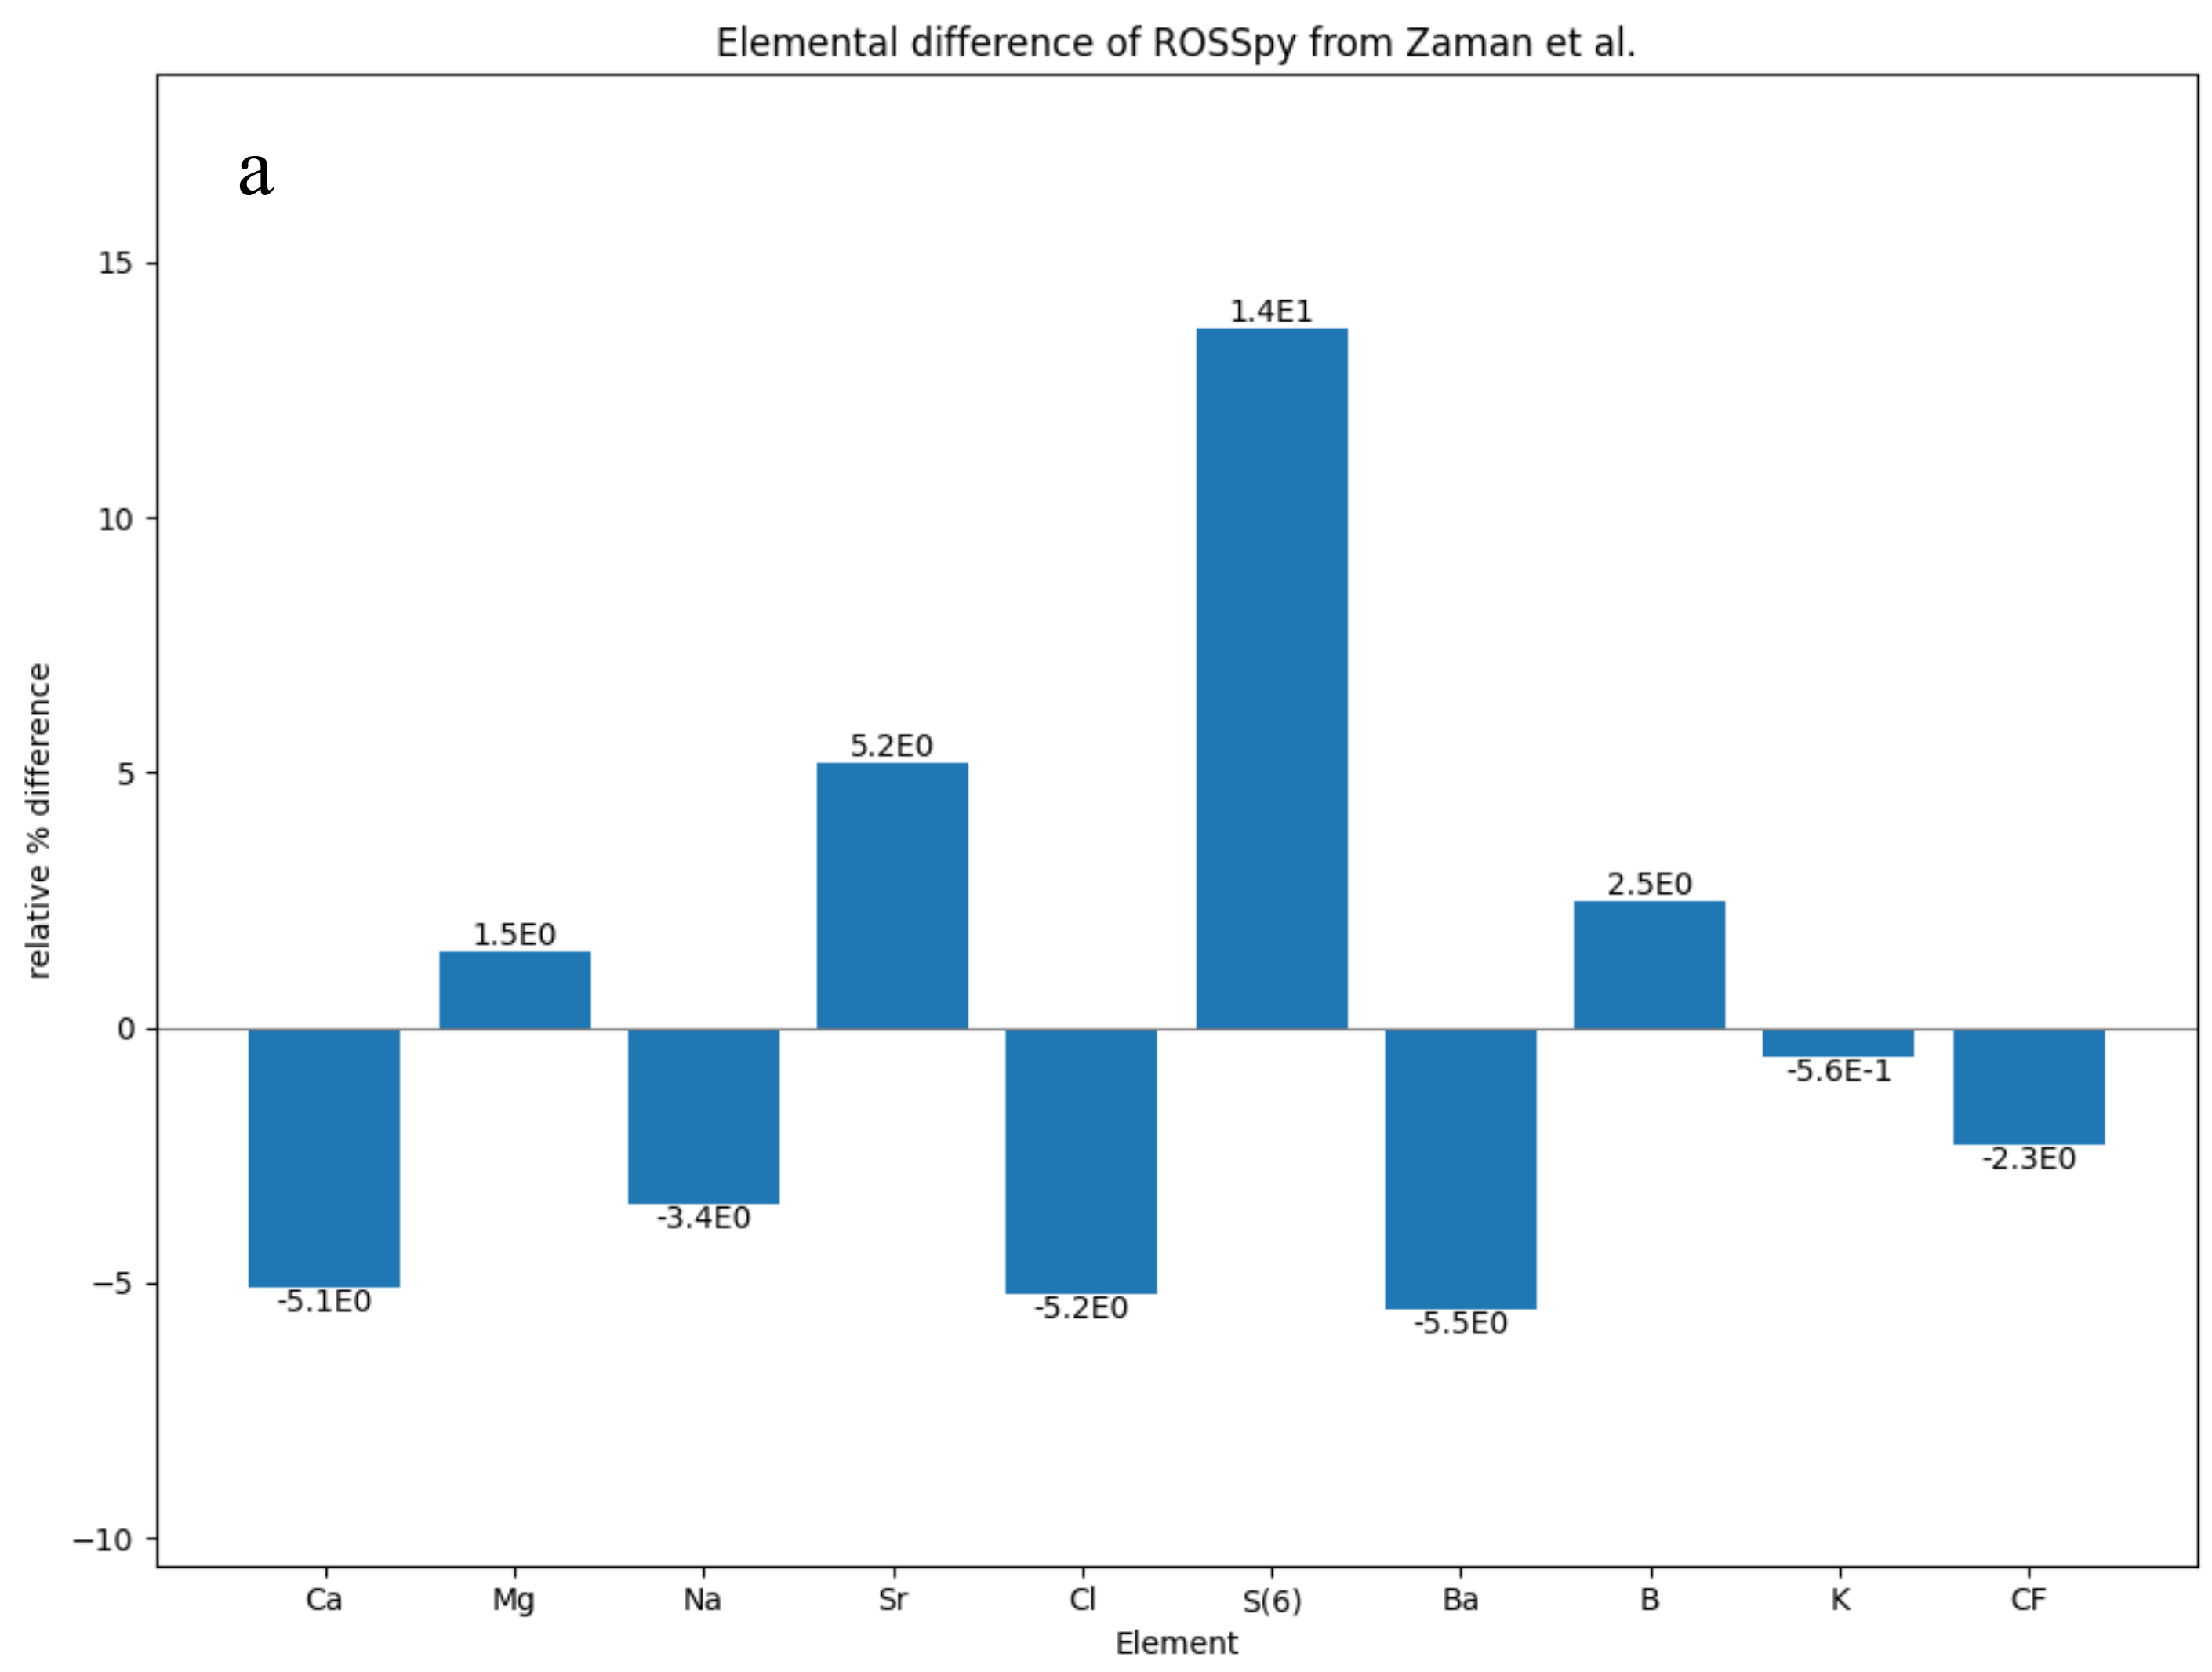
\includegraphics[width=\linewidth]{images/ROSSpy/case_studies/Zaman_comparison.png}} \\ \midrule
        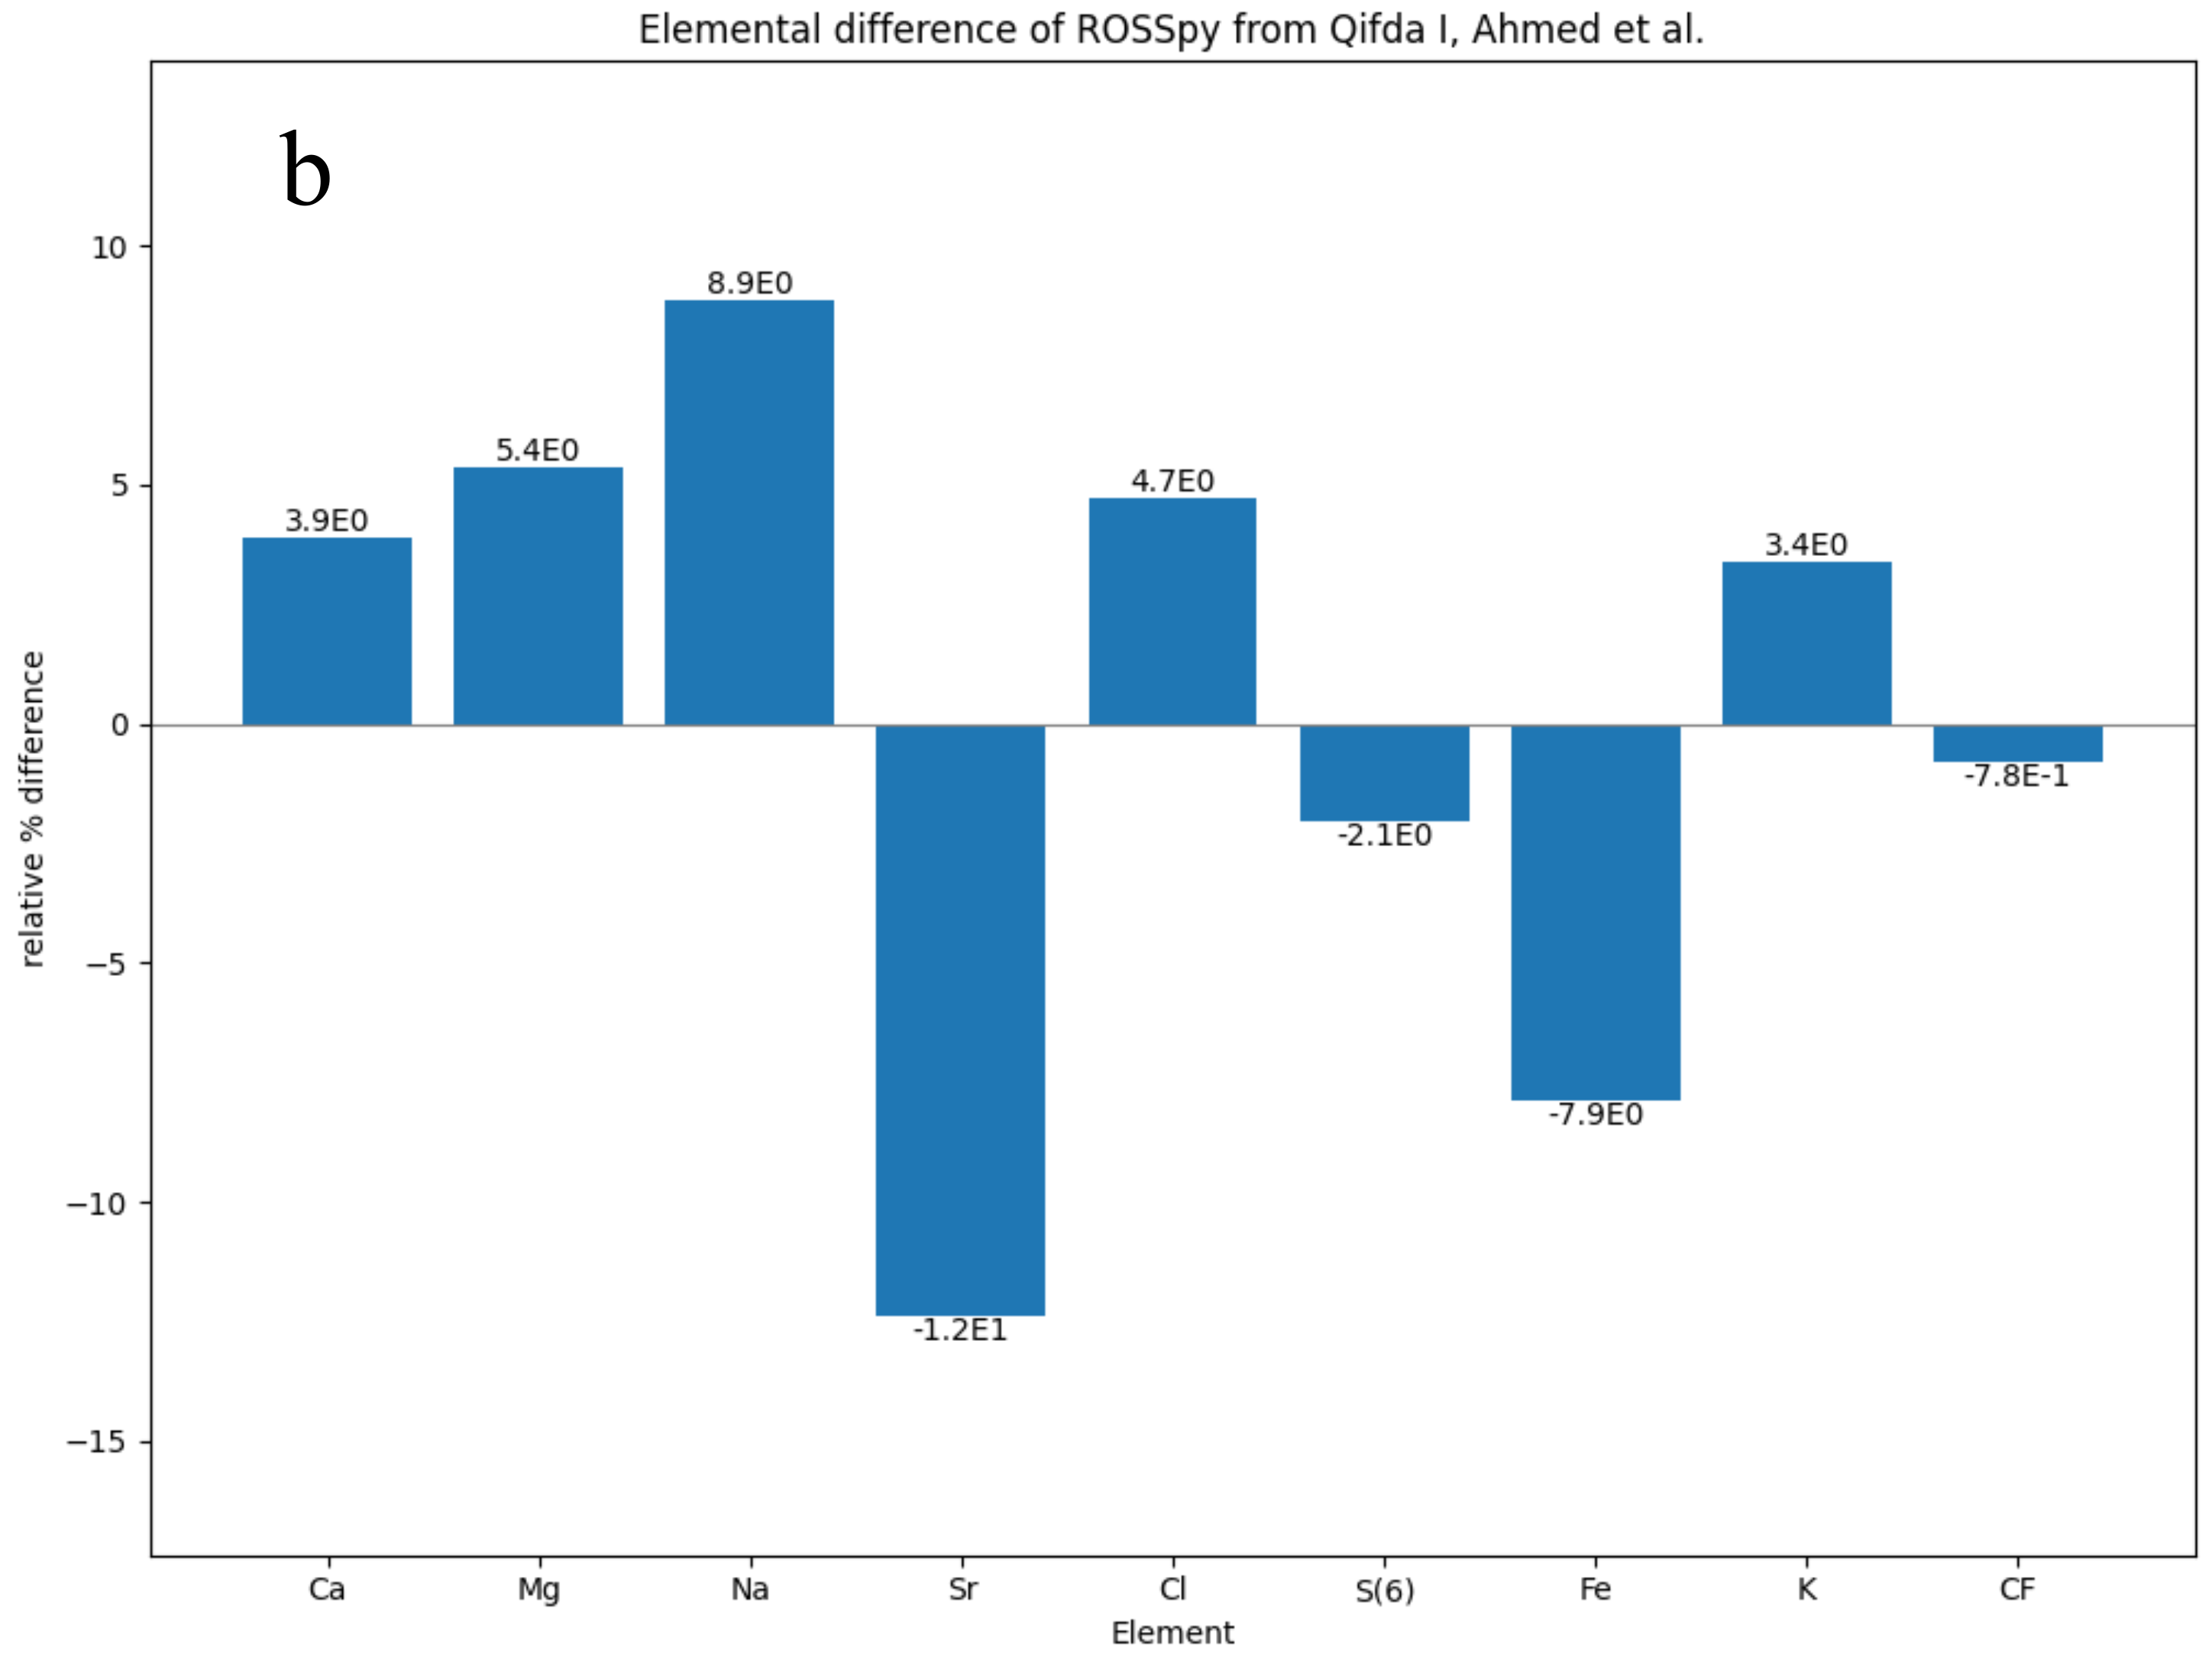
\includegraphics[width=0.49\linewidth]{images/ROSSpy/case_studies/Ahmed_comparison.png} & 
        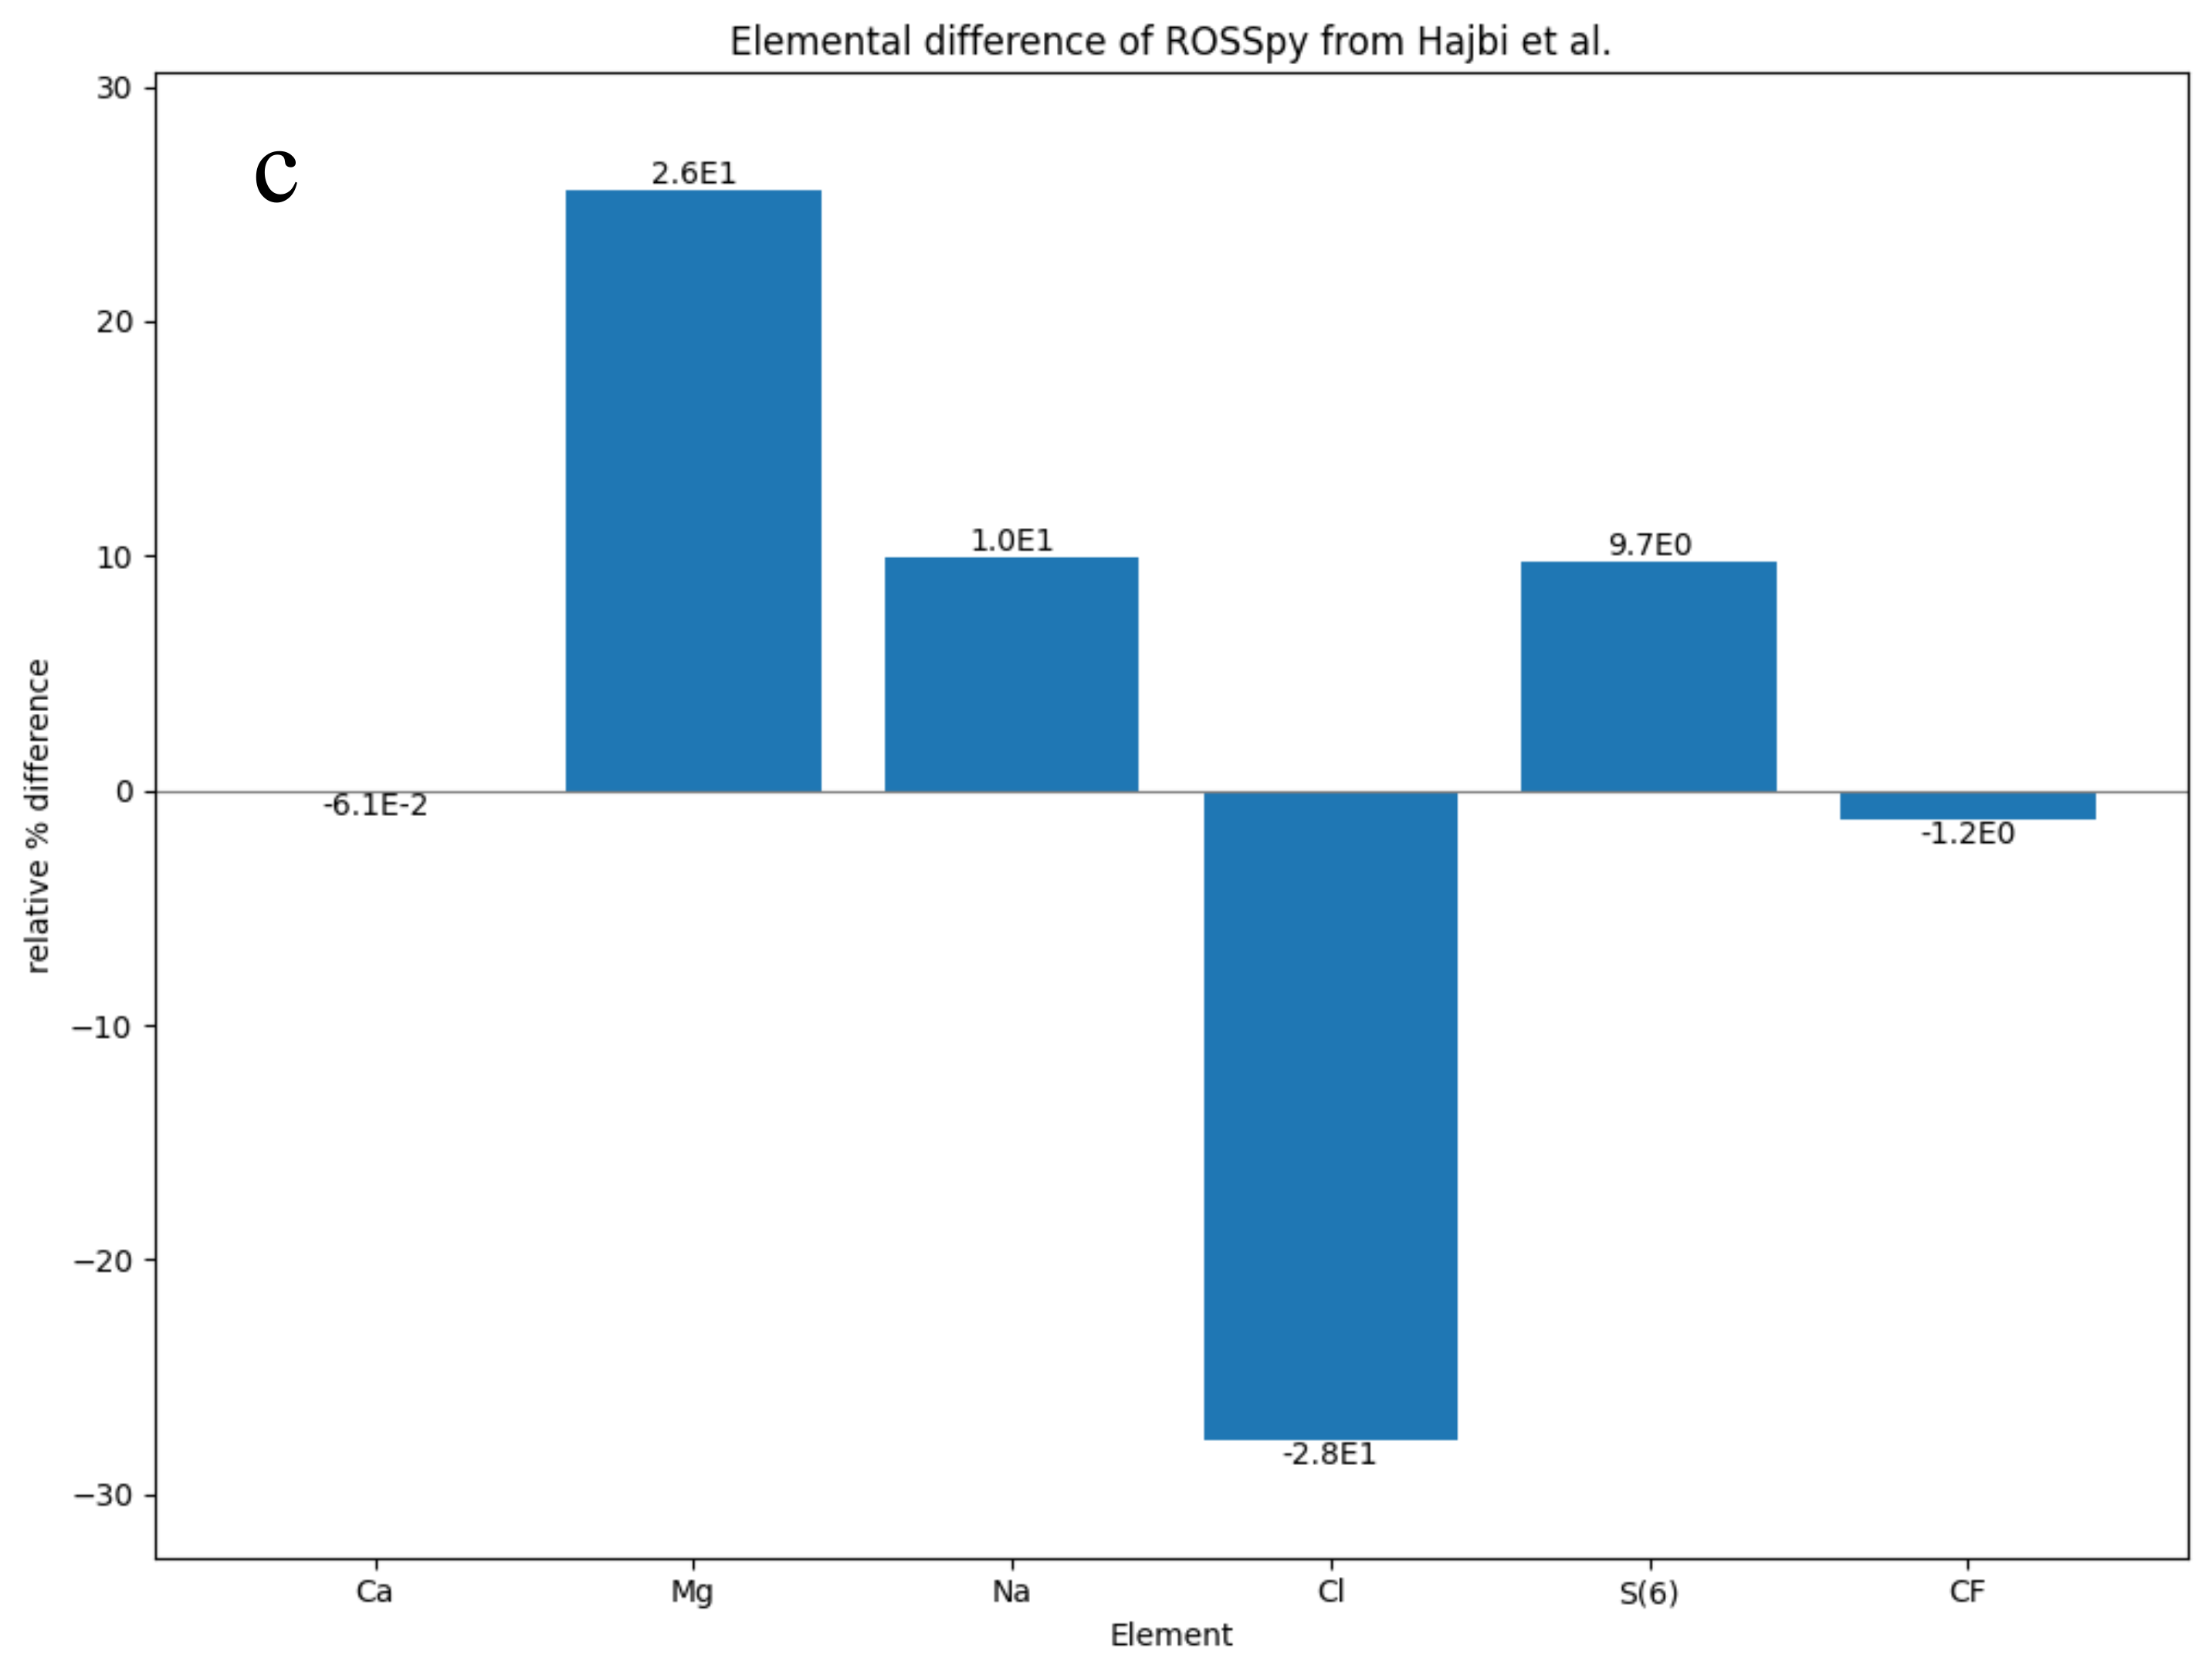
\includegraphics[width=0.49\linewidth]{images/ROSSpy/case_studies/Hajbi_comparison.png} \\ \bottomrule
    \end{tabular}
    \caption{
        The \%-error between predicted and experimental brine concentrations from RO plants. Panels a-c) correspond to comparisons with the Zaman et al. \cite{Zaman2015DownstreamCompounds}, Ahmed et al. \cite{Ahmed2001BrineEmirates}, and Hajbi et al. \cite{Hajbi2010ReuseBrine} studies, respectively, and each possess different y-axis scales to best resolve the bars in each graph. The trend is that prediction accuracy is proportional to the quantity of parameterized ions. 
    }
    \label{bar_graphs}
\end{figure}


\subsection{Scaling}
The scaling predictions were verified qualitatively from experimental literature and quantitatively from theoretical calculations, since experimental literature that quantified scalants with feed geochemistry was not discovered.

\subsubsection{Quantitative}
The quantitative verification consisted of two simple cases of Gypsum precipitation. 1) The first case in Table \ref{gypsum_ice_table} consists of a solution with only $Ca^{2+}$ and $SO_4^{2-}$, where the ionic concentrations decreased by $0.01859$ moles while $0.01961$ moles of Gypsum precipitated. This 5\% discrepancy in mass balance is attributed to the printed PHREEQC values in this calculation neglecting diffusion within the feed solution, yet diffusion is considered in the final output of PHREEQC. 2) The second case in Table S1 evaluates Gypsum precipitation from desalinating the solution from the first case with that from the Red Sea, which only precipitates Gypsum in our model. The simple solution precipitated $0.181$ moles of Gypsum, while the Red Sea precipitated $0.194$ moles. This $+7\%$-error is attributed to ionic interactions within the Red Sea feed that are not present by the simple solution of only $Ca^{2+}$ and $SO_4^{2-}$. These subtle $[5,7]\%$ deviations, even without considering the coarse assumptions in these simple examples, are relatively minor in the context of other sources of error, such as feed measurements, and still elicit quantitative consistency in scaling predictions.

\begin{table}
    \centering
    \begin{tabular}{c|ccccc}
      \toprule
       & $Ca^{2+}$ & $+$ & $SO_4^{2-}$ & $\leftrightharpoons$ & $CaSO_4$ \\
      \midrule
      I & $0.3545$ && $1.816$ && $0$ \\
      C & $-0.01859$ && $-0.01859$ && $+0.01961$ \\
      F & $0.3360$ && $1.797$ && $0.01961$ \\
      \bottomrule
    \end{tabular}
    \caption{
        Gypsum precipitation according to the ICE (Initial, Change, Equilibrium) framework, except that "Equilibrium" (E) is replaced with "Final" (F) since the system does not completely reach equilibrium within the RO module. The $5\%-error$ in row C, between the changes in ionic and Gypsum moles, suggests a subtle discrepancy in mass balance of PHREEQC; however, this is attributed to PHREEQC printing values before diffusion is incorporated in the calculations, per David Parkhurst. 
      }
    \label{gypsum_ice_table}
\end{table}

\subsubsection{Qualitative}
The scaling predictions were qualitatively verified through three experimental studies. 

\paragraph{Karabelas et al., 2020 \cite{Karabelas2020ScalingTools}}
This study inspired features of ROSSpy by reviewing the state-of-the-art, and future directions, for predictive scaling software. The study also, importantly, describes in its Supporting Information scalants that were observed after desalination with defined conditions. Scaling predictions from these conditions in Figure \ref{qualitative_scaling}a, over a few PHREEQC databases, match the reported scalants ("Calcite but not Gypsum" and a "few other salts, such as Barite and Dolomite, could also deposit at downstream...") in numerous aspects: 1) Calcite was the primary scalant; 2) Gypsum was not observed; 3) a few other salts precipitated, including Dolomite and Barite, depending upon the PHREEQC database; and 4) these other salts precipitated primarily in the downstream portion of the module.  

\paragraph{Karabelas et al., 2014 \cite{Karabelas2014IncipientChannels}}
This study elucidates the mechanisms of incipient scaling from RO desalination -- with Gypsum as the archetypal scalant \cite{Lyster2009CoupledModule}. The ID 28SC trial, which was the most thoroughly described trial, was simulated and Gypsum was the only predicted scalant in Figure \ref{qualitative_scaling}b, just as the reported scalant.  

\paragraph{Lee et al., 2009 \cite{Lee2009MembraneWastewater}}
This study evaluates the use of a membrane bioreactor -- a hollow-fiber membrane module design that is mechanistically similar to RO and thus can be represented by our model -- to treat wastewater. The wastewater filtration system was simulated, and the only predicted scalant was Calcite in Figure \ref{qualitative_scaling}c, just as the reported scalant.

\begin{figure}
    \begin{tabular}{c|c}
        \multicolumn{2}{c}{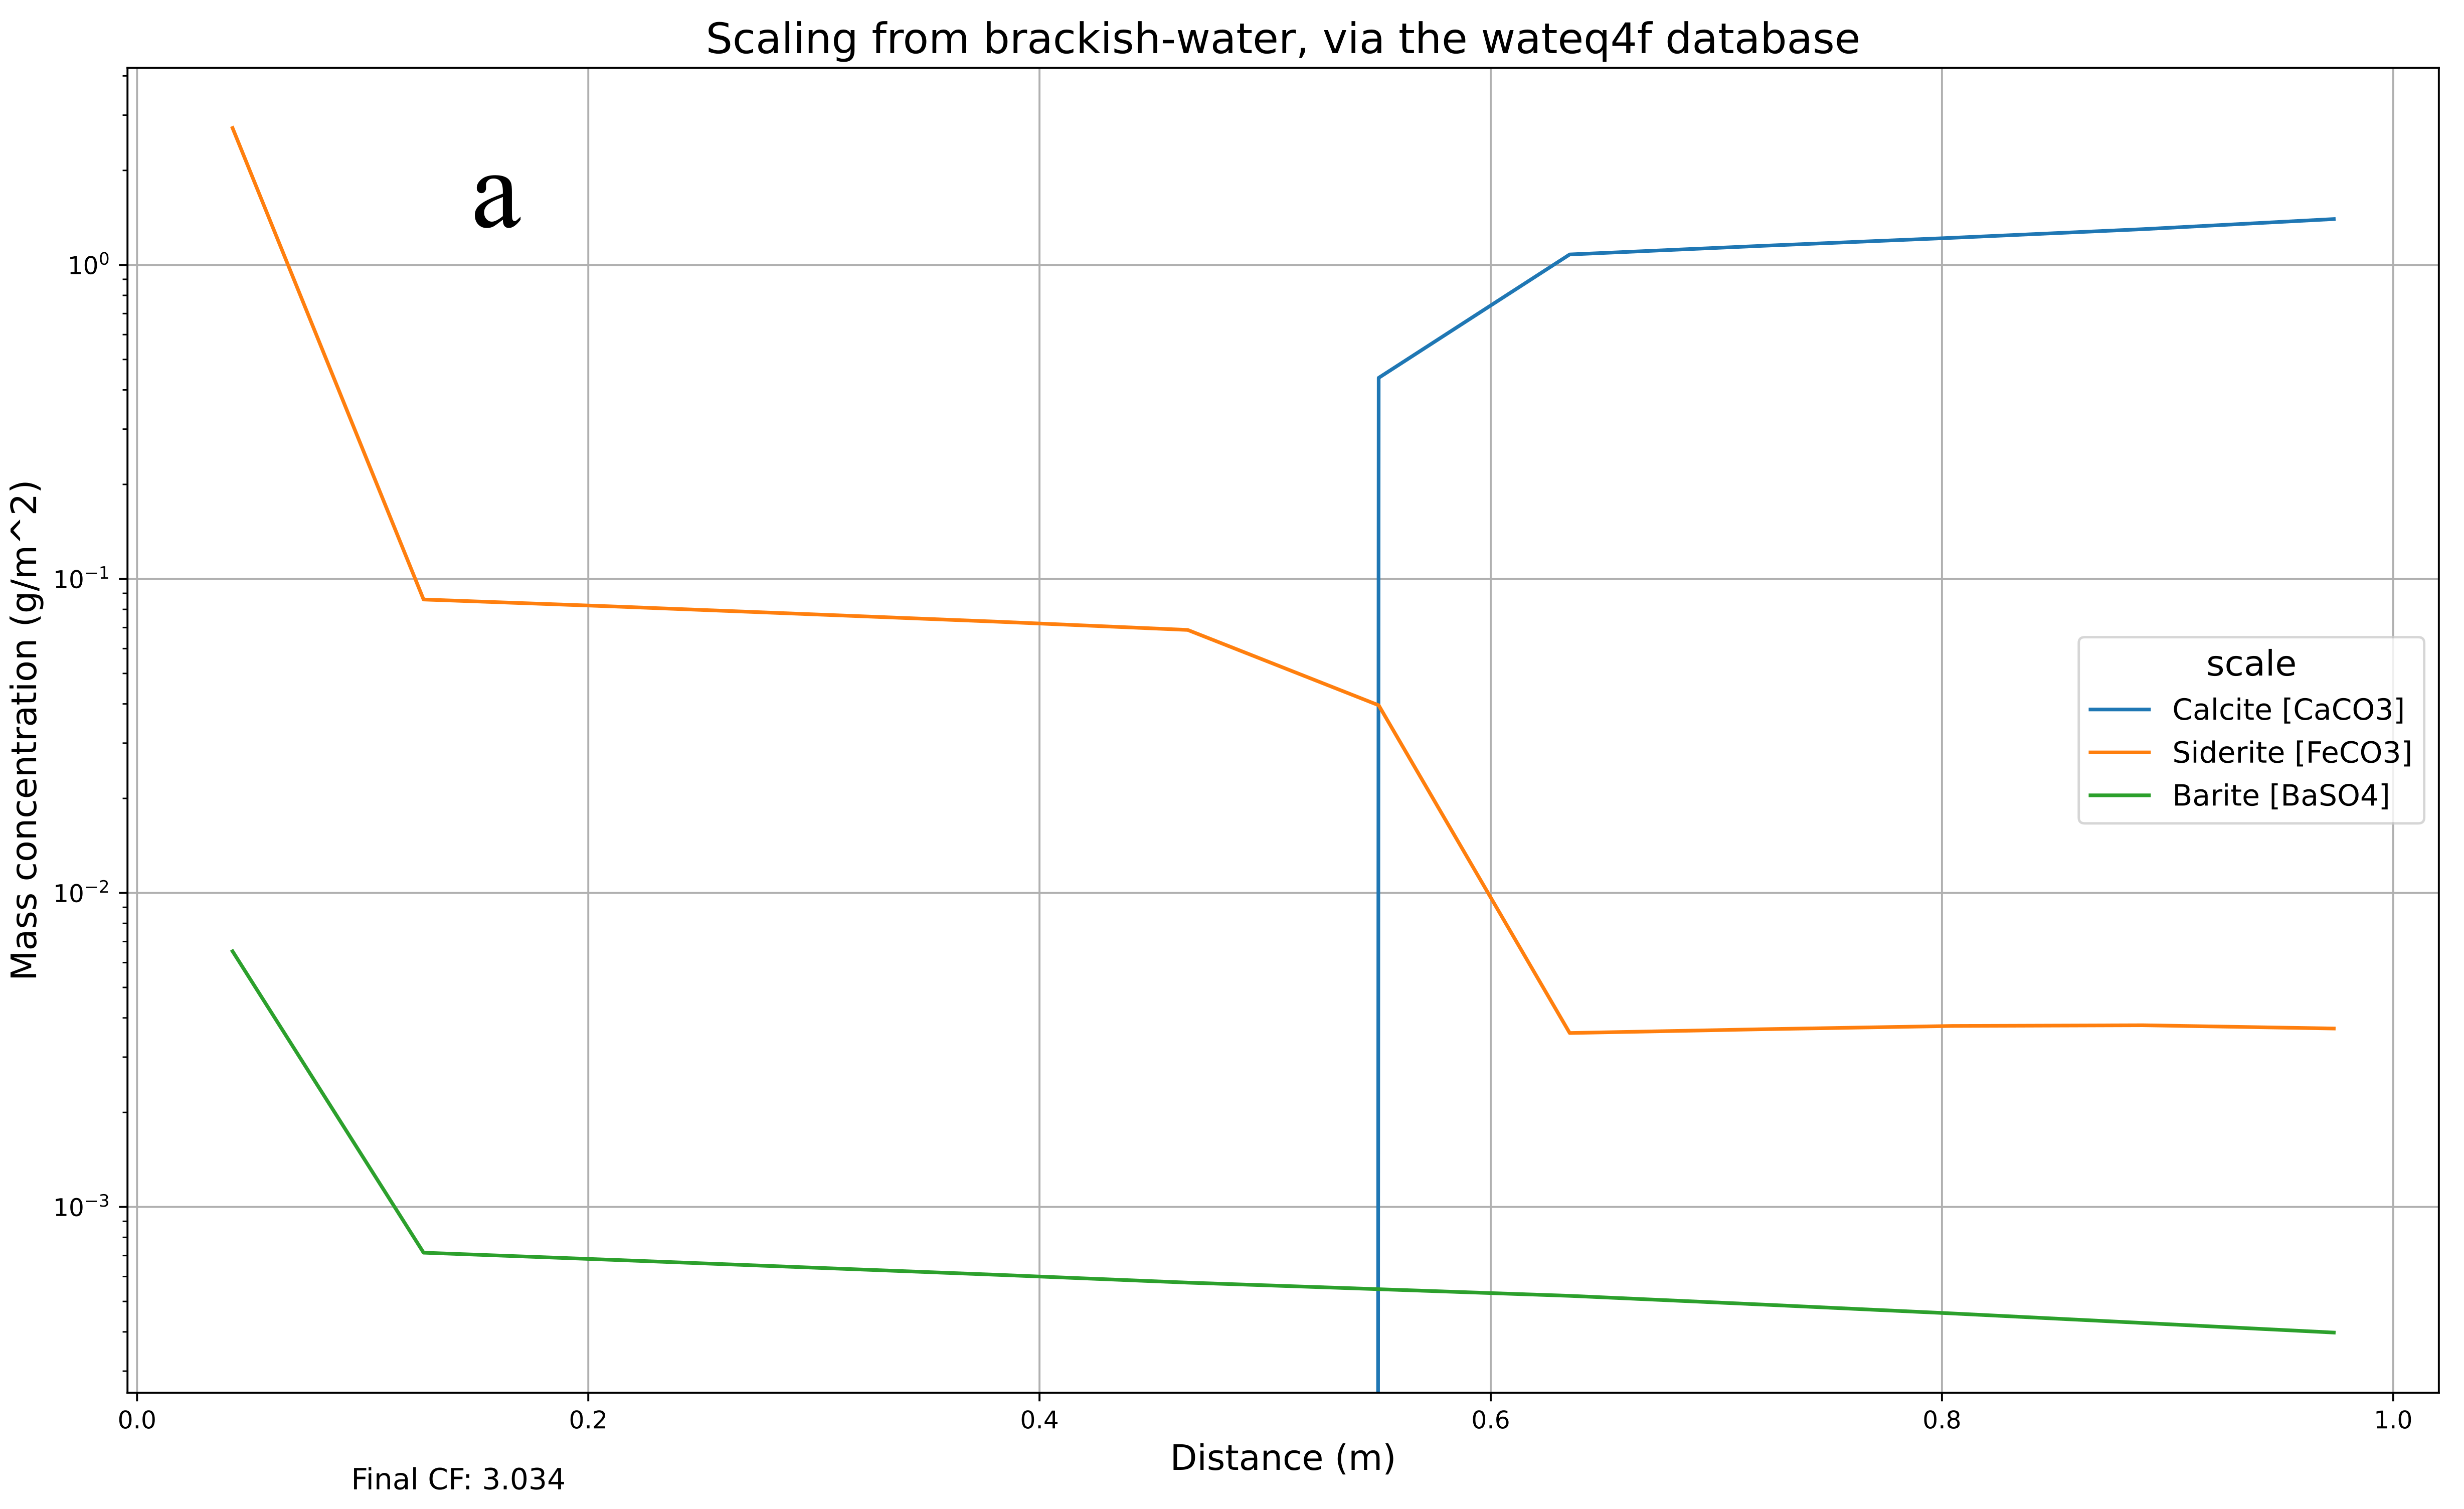
\includegraphics[width=\linewidth]{images/ROSSpy/case_studies/Karabelas_2020_wateq4f.png}} \\
        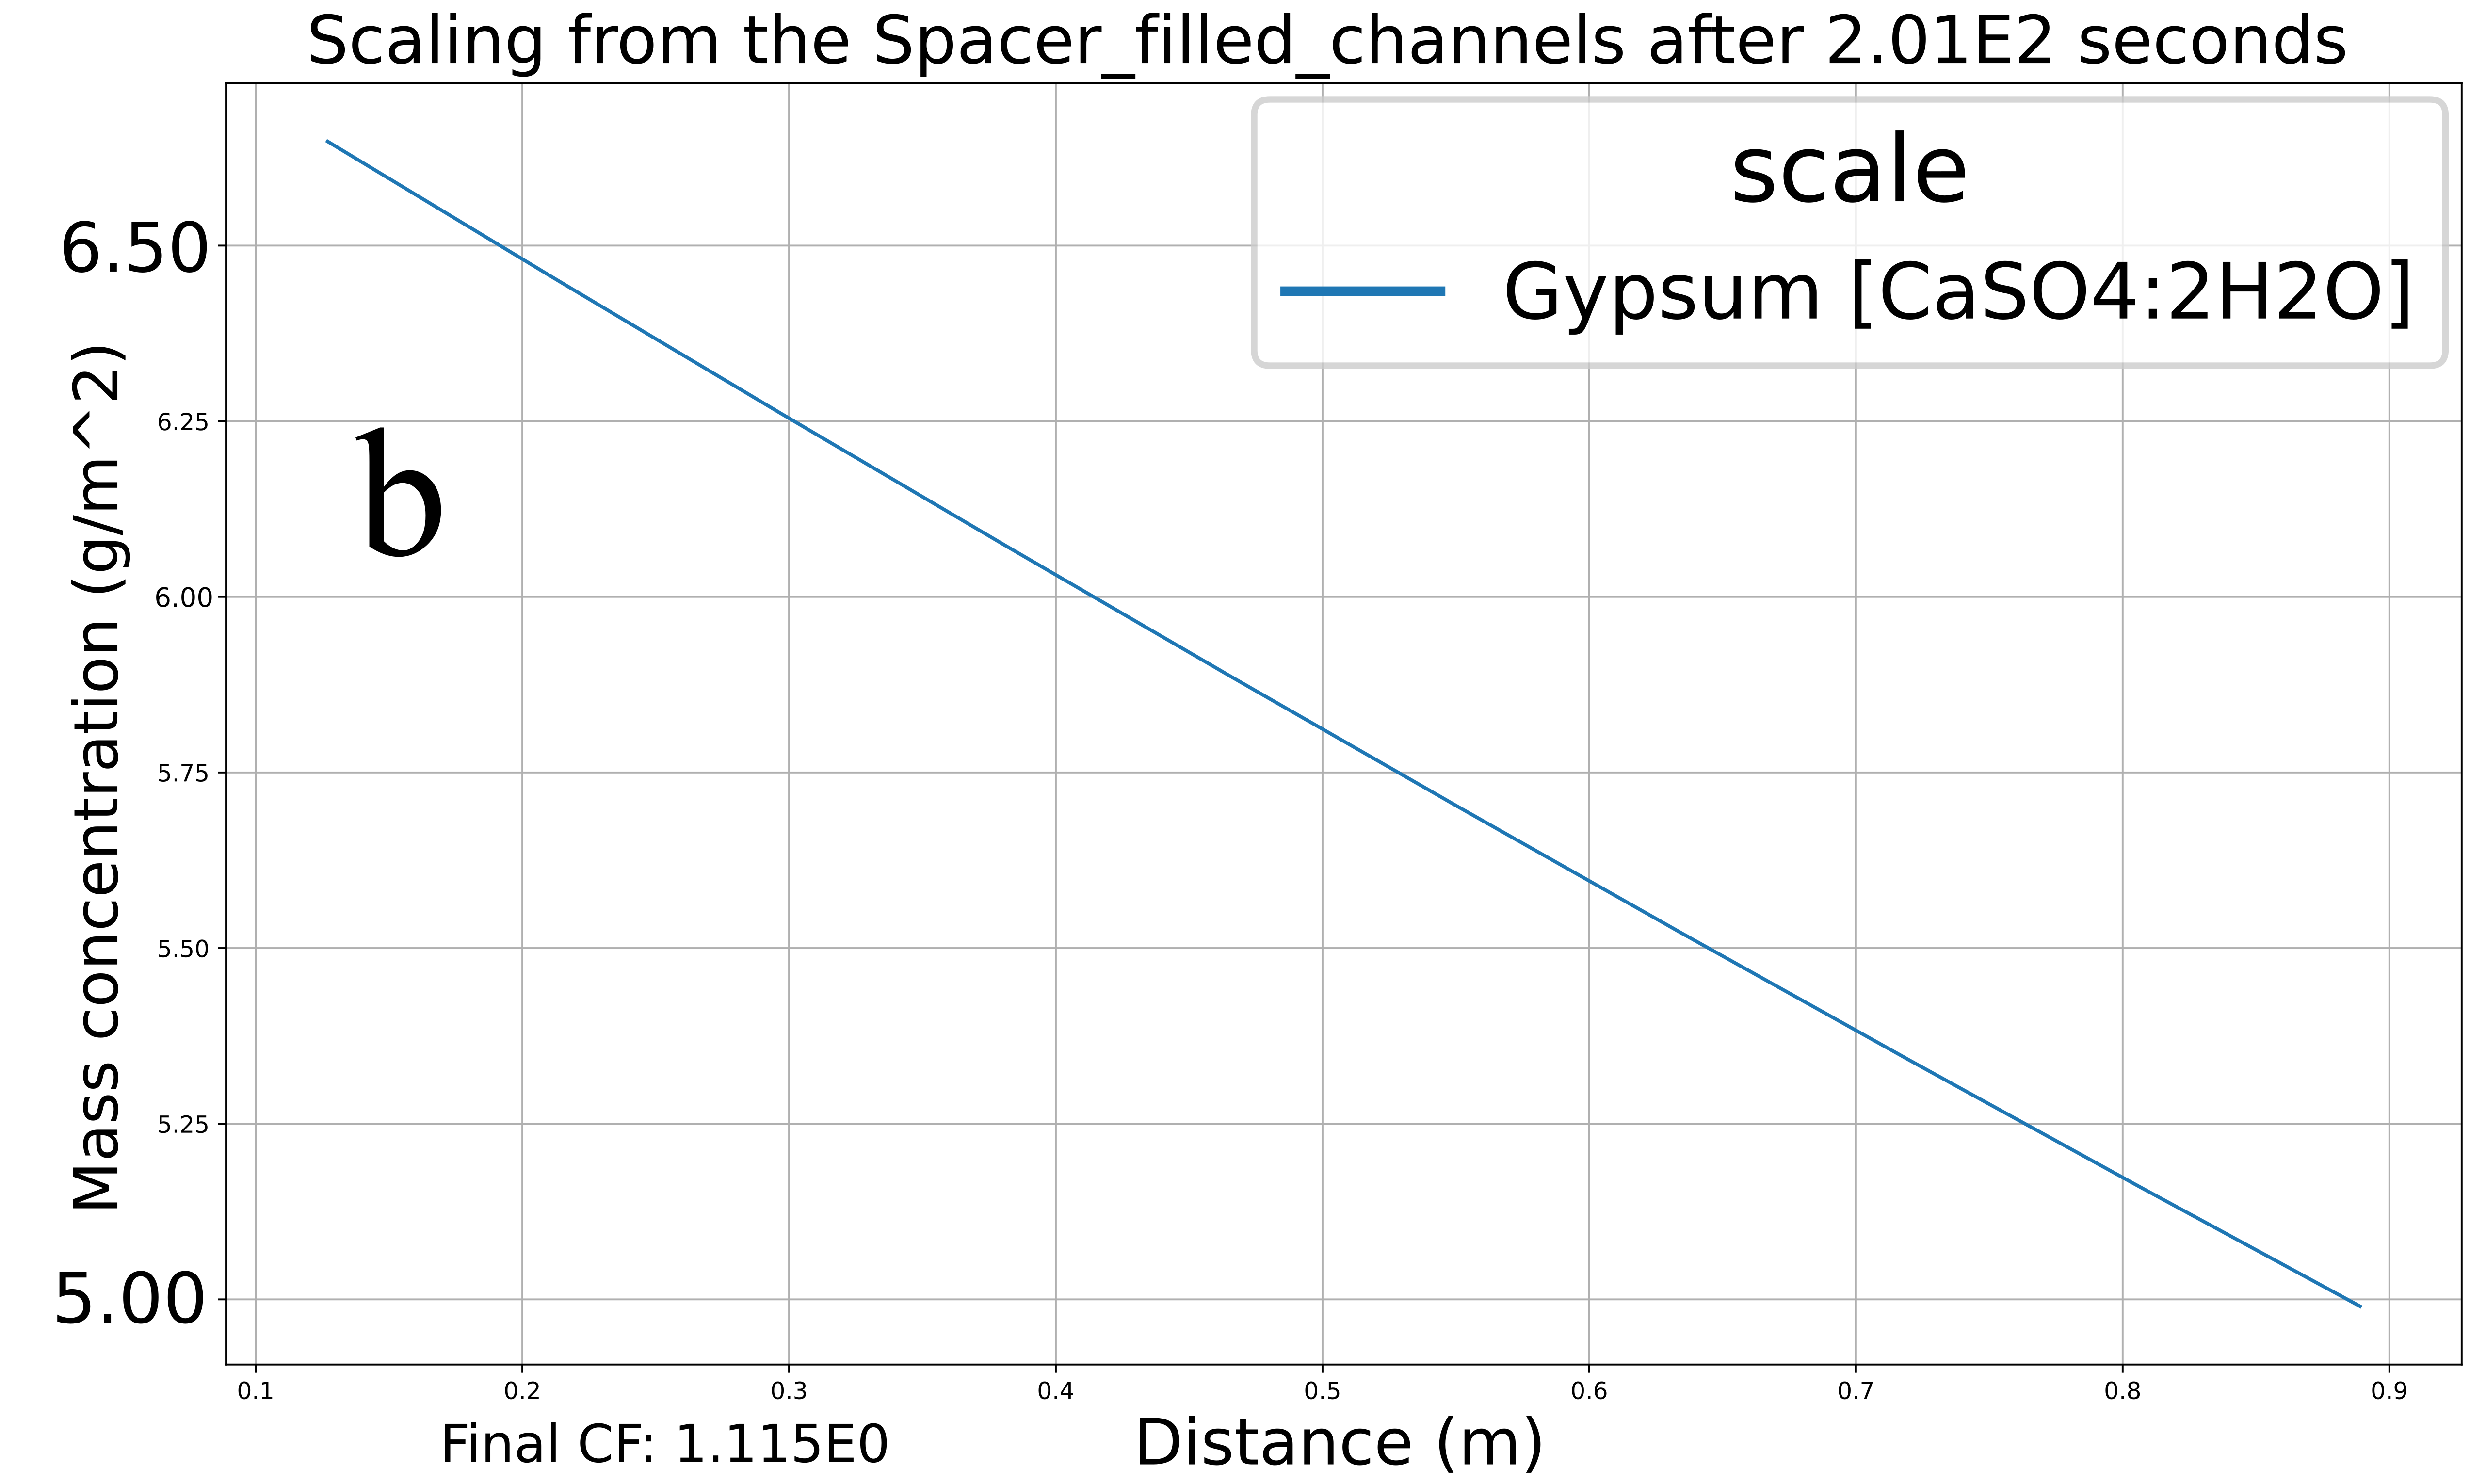
\includegraphics[width=0.49\linewidth]{images/ROSSpy/case_studies/Karabelas_2014_pitzer.png} 
        & 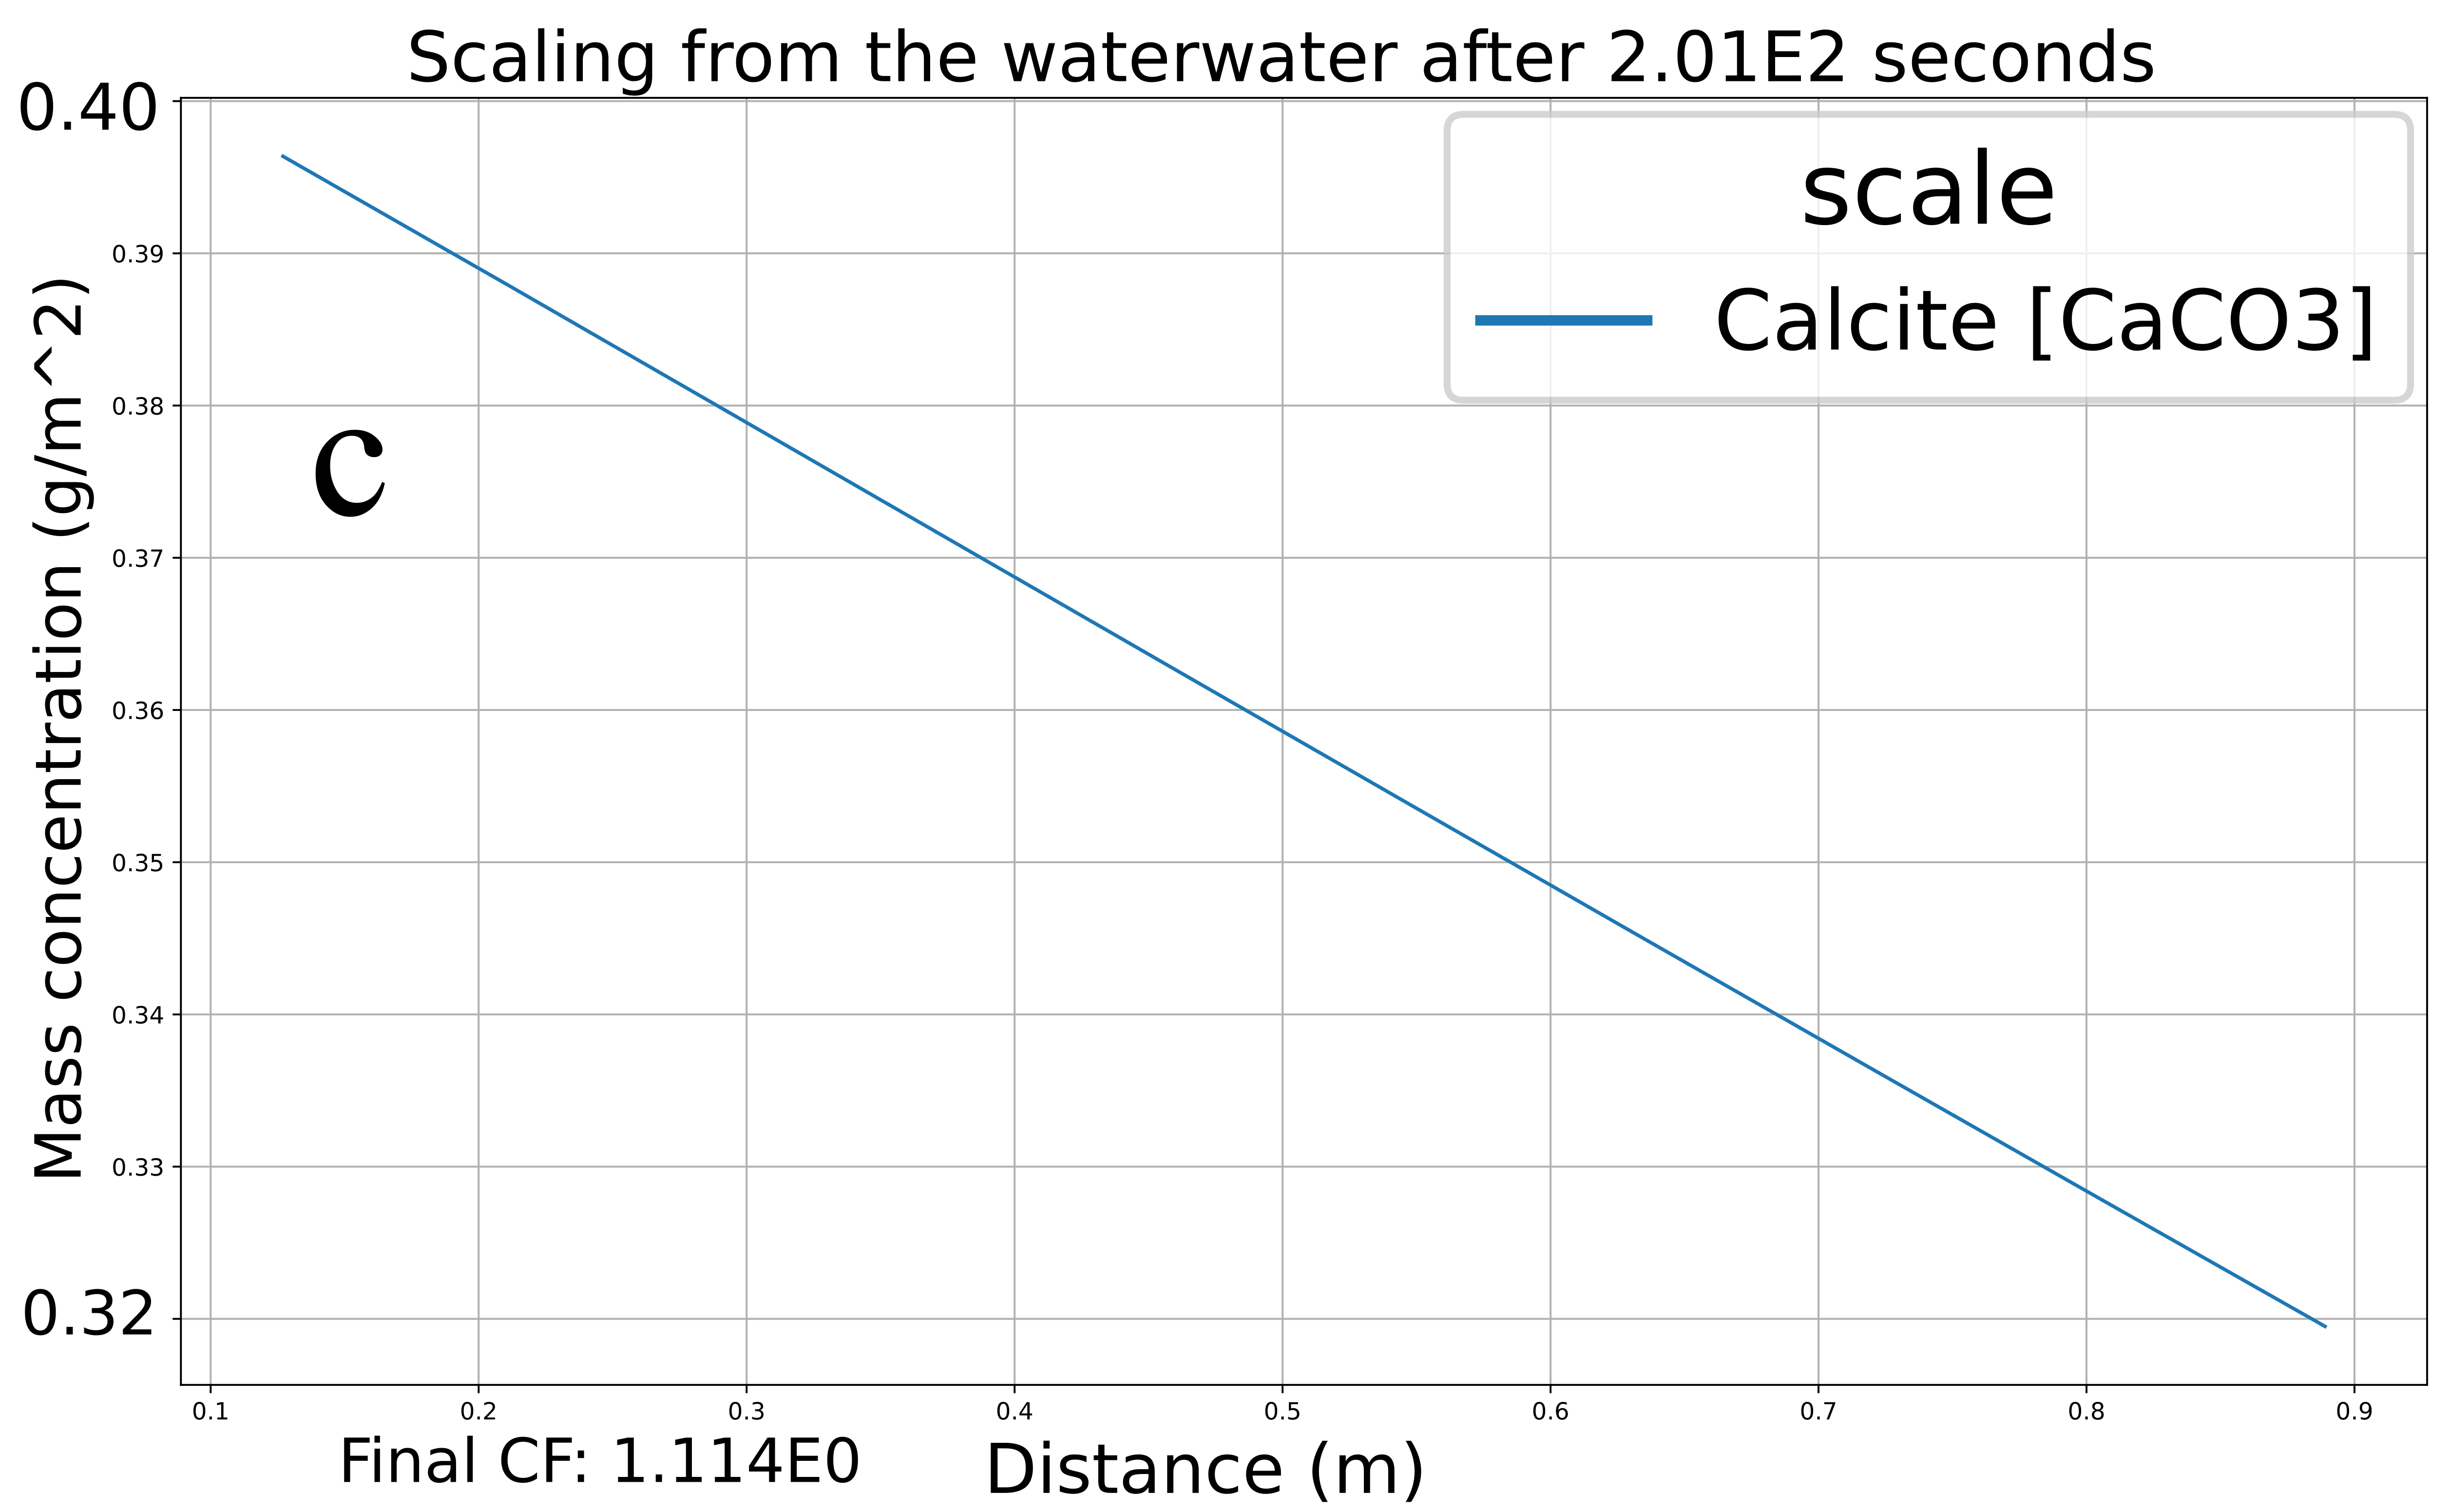
\includegraphics[width=0.49\linewidth]{images/ROSSpy/case_studies/Lee_pitzer.png} \\
    \end{tabular}
    \caption{
        The qualitative validation of scaling for a) multiple minerals from the Karabelas et al., 2020 study; b) Gypsum in the Karabelas et al., 2014 study; and c) Calcite in the Lee et al. study. 
    }
    \label{qualitative_scaling}
\end{figure}


\section{Sensitivity analyses}
A few sensitivity analyses were conducted with major variables in the following subsections. Additional sensitivity analyses of lesser parameters are presented in the Supporting Information.

\subsection{Database section}
The PHREEQC databases crucially 1) determines the set of minerals that can be simulated; 2) contains all of the kinetic, thermodynamic, and stoichiometric information of each mineral; and 3) employs a chemical activity model: e.g. Pitzer, Debye-H\"uckel, and Davies in Section 7 of the Supporting Information. The Pitzer model \cite{Pitzer1973ThermodynamicsEquations,Pitzer1974ThermodynamicsElectrolytes}, which is implemented in the pitzer PHREEQC database, is touted as being supremely accurate in the concentration range of desalination \cite{VandeLisdonk2001PredictionSystems,Sheikholeslami2004AssessmentUnits,Mohammad2007PredictionMembranes}; however, the narrow breadth of accepted ions and minerals may justify using other databases, such as wateq4, for complex or uncommon feed sources. Each of the 13 databases were simulated in desalinating the Red Sea, where the $Amm$, $Core10$, $LLNL$, and $Minteq.v4$ databases failed to numerically converge while the scaling predictions from the other $\frac{9}{13}$ databases are summarized in Figure \ref{database_selection}. The database selection evidently alters scaling predictions; thus, the database must be carefully selected for a given system after reviewing the PHREEQC User Manual or inquirying to the PHREEQC user forum \url{PHREEQCusers.org}.

\begin{figure}
    \centering
    \begin{tabular}{c|c}
        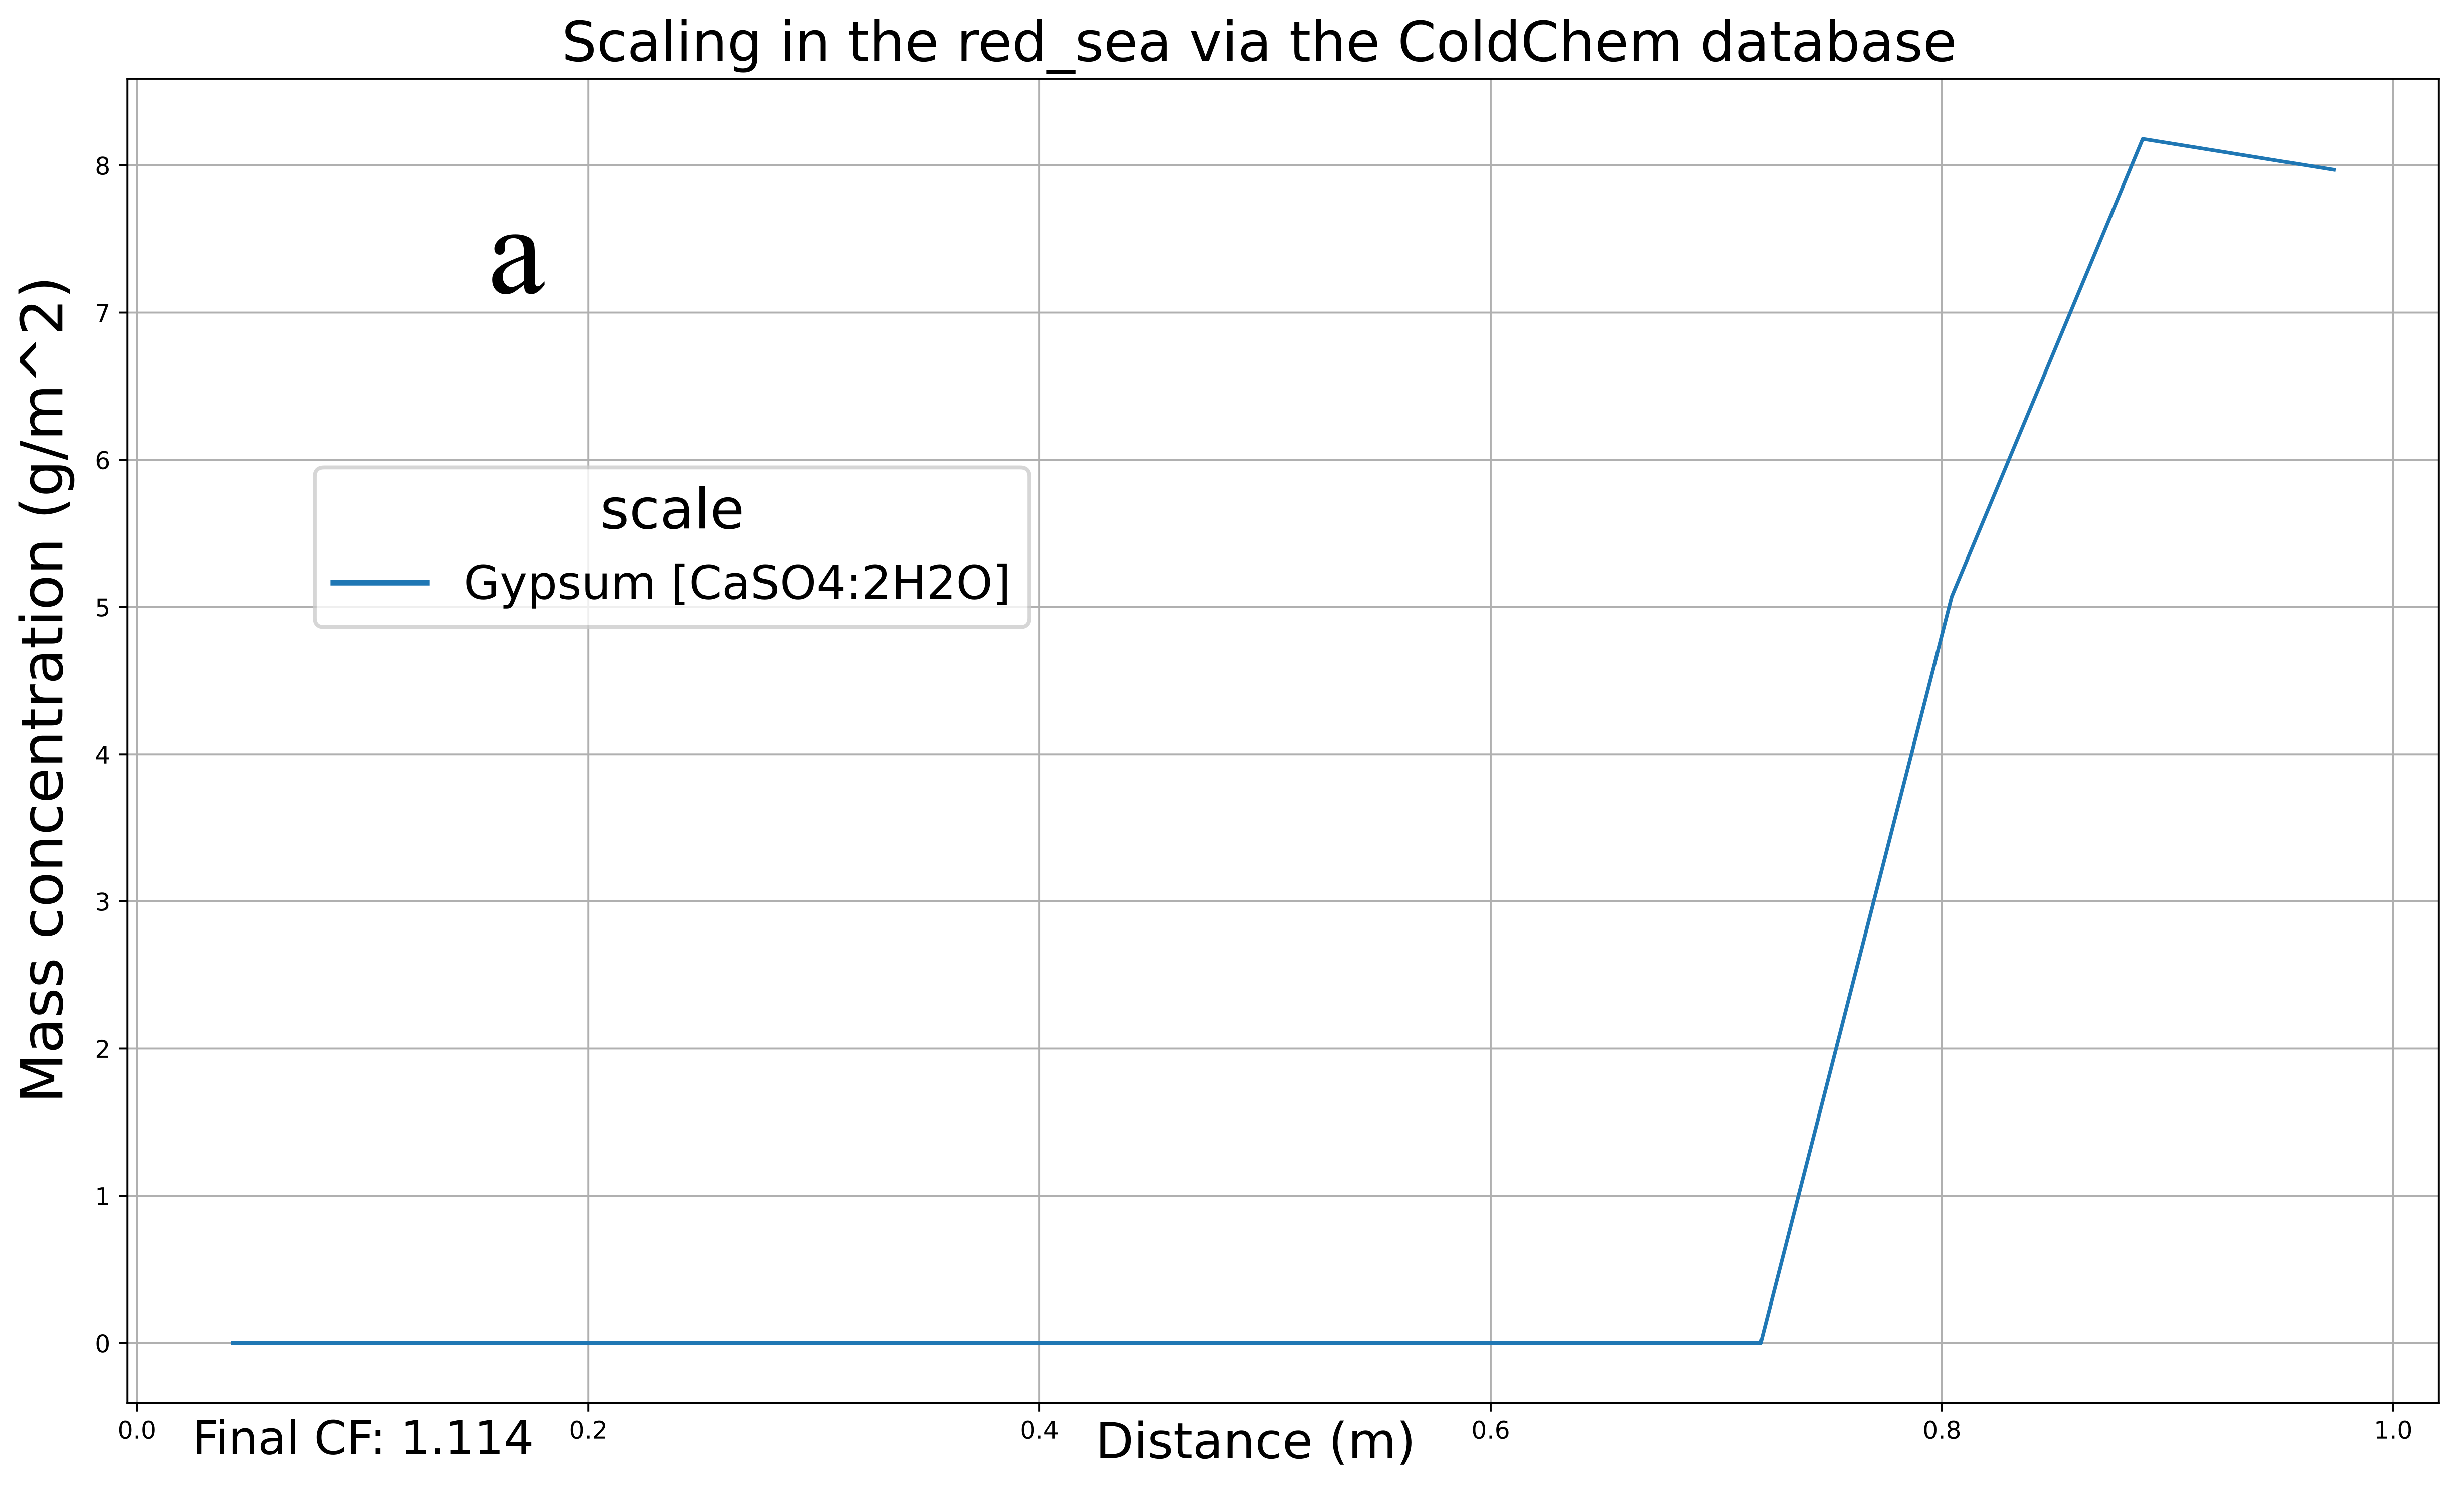
\includegraphics[width=0.49\textwidth]{images/ROSSpy/sensitivity_analyses/databases/ColdChem.png} 
        & 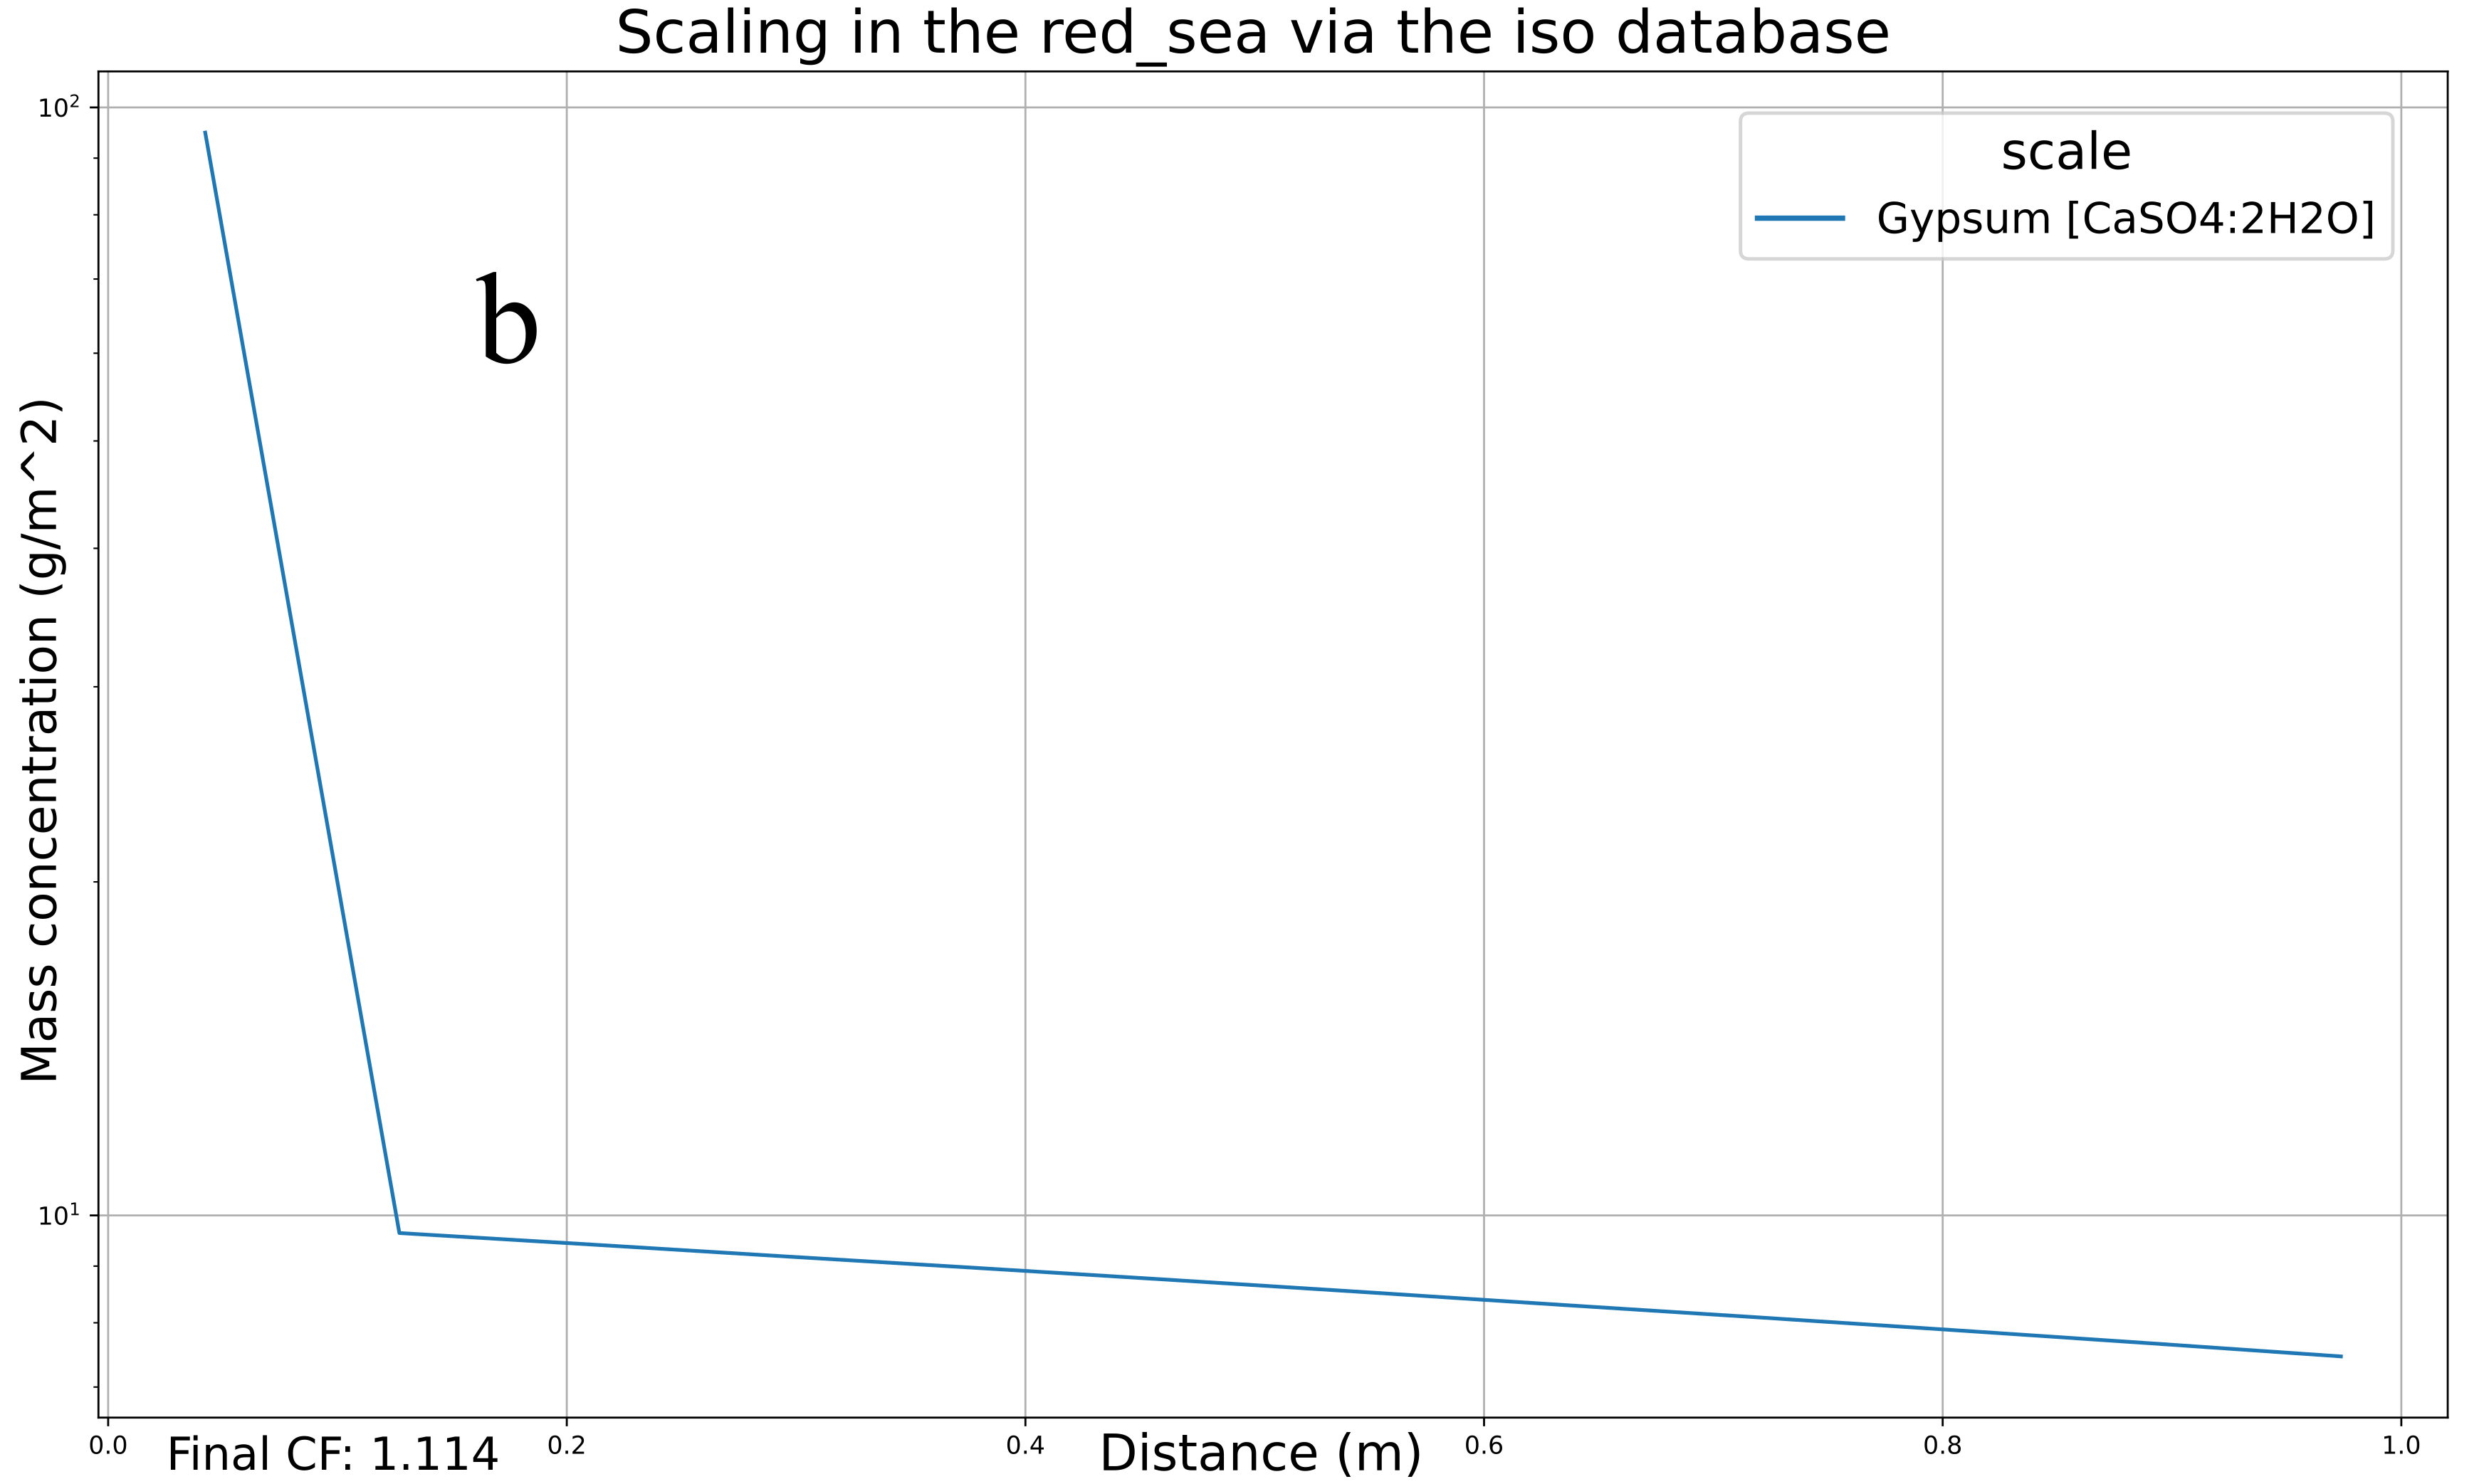
\includegraphics[width=0.49\textwidth]{images/ROSSpy/sensitivity_analyses/databases/Iso.png} \\ \midrule 
        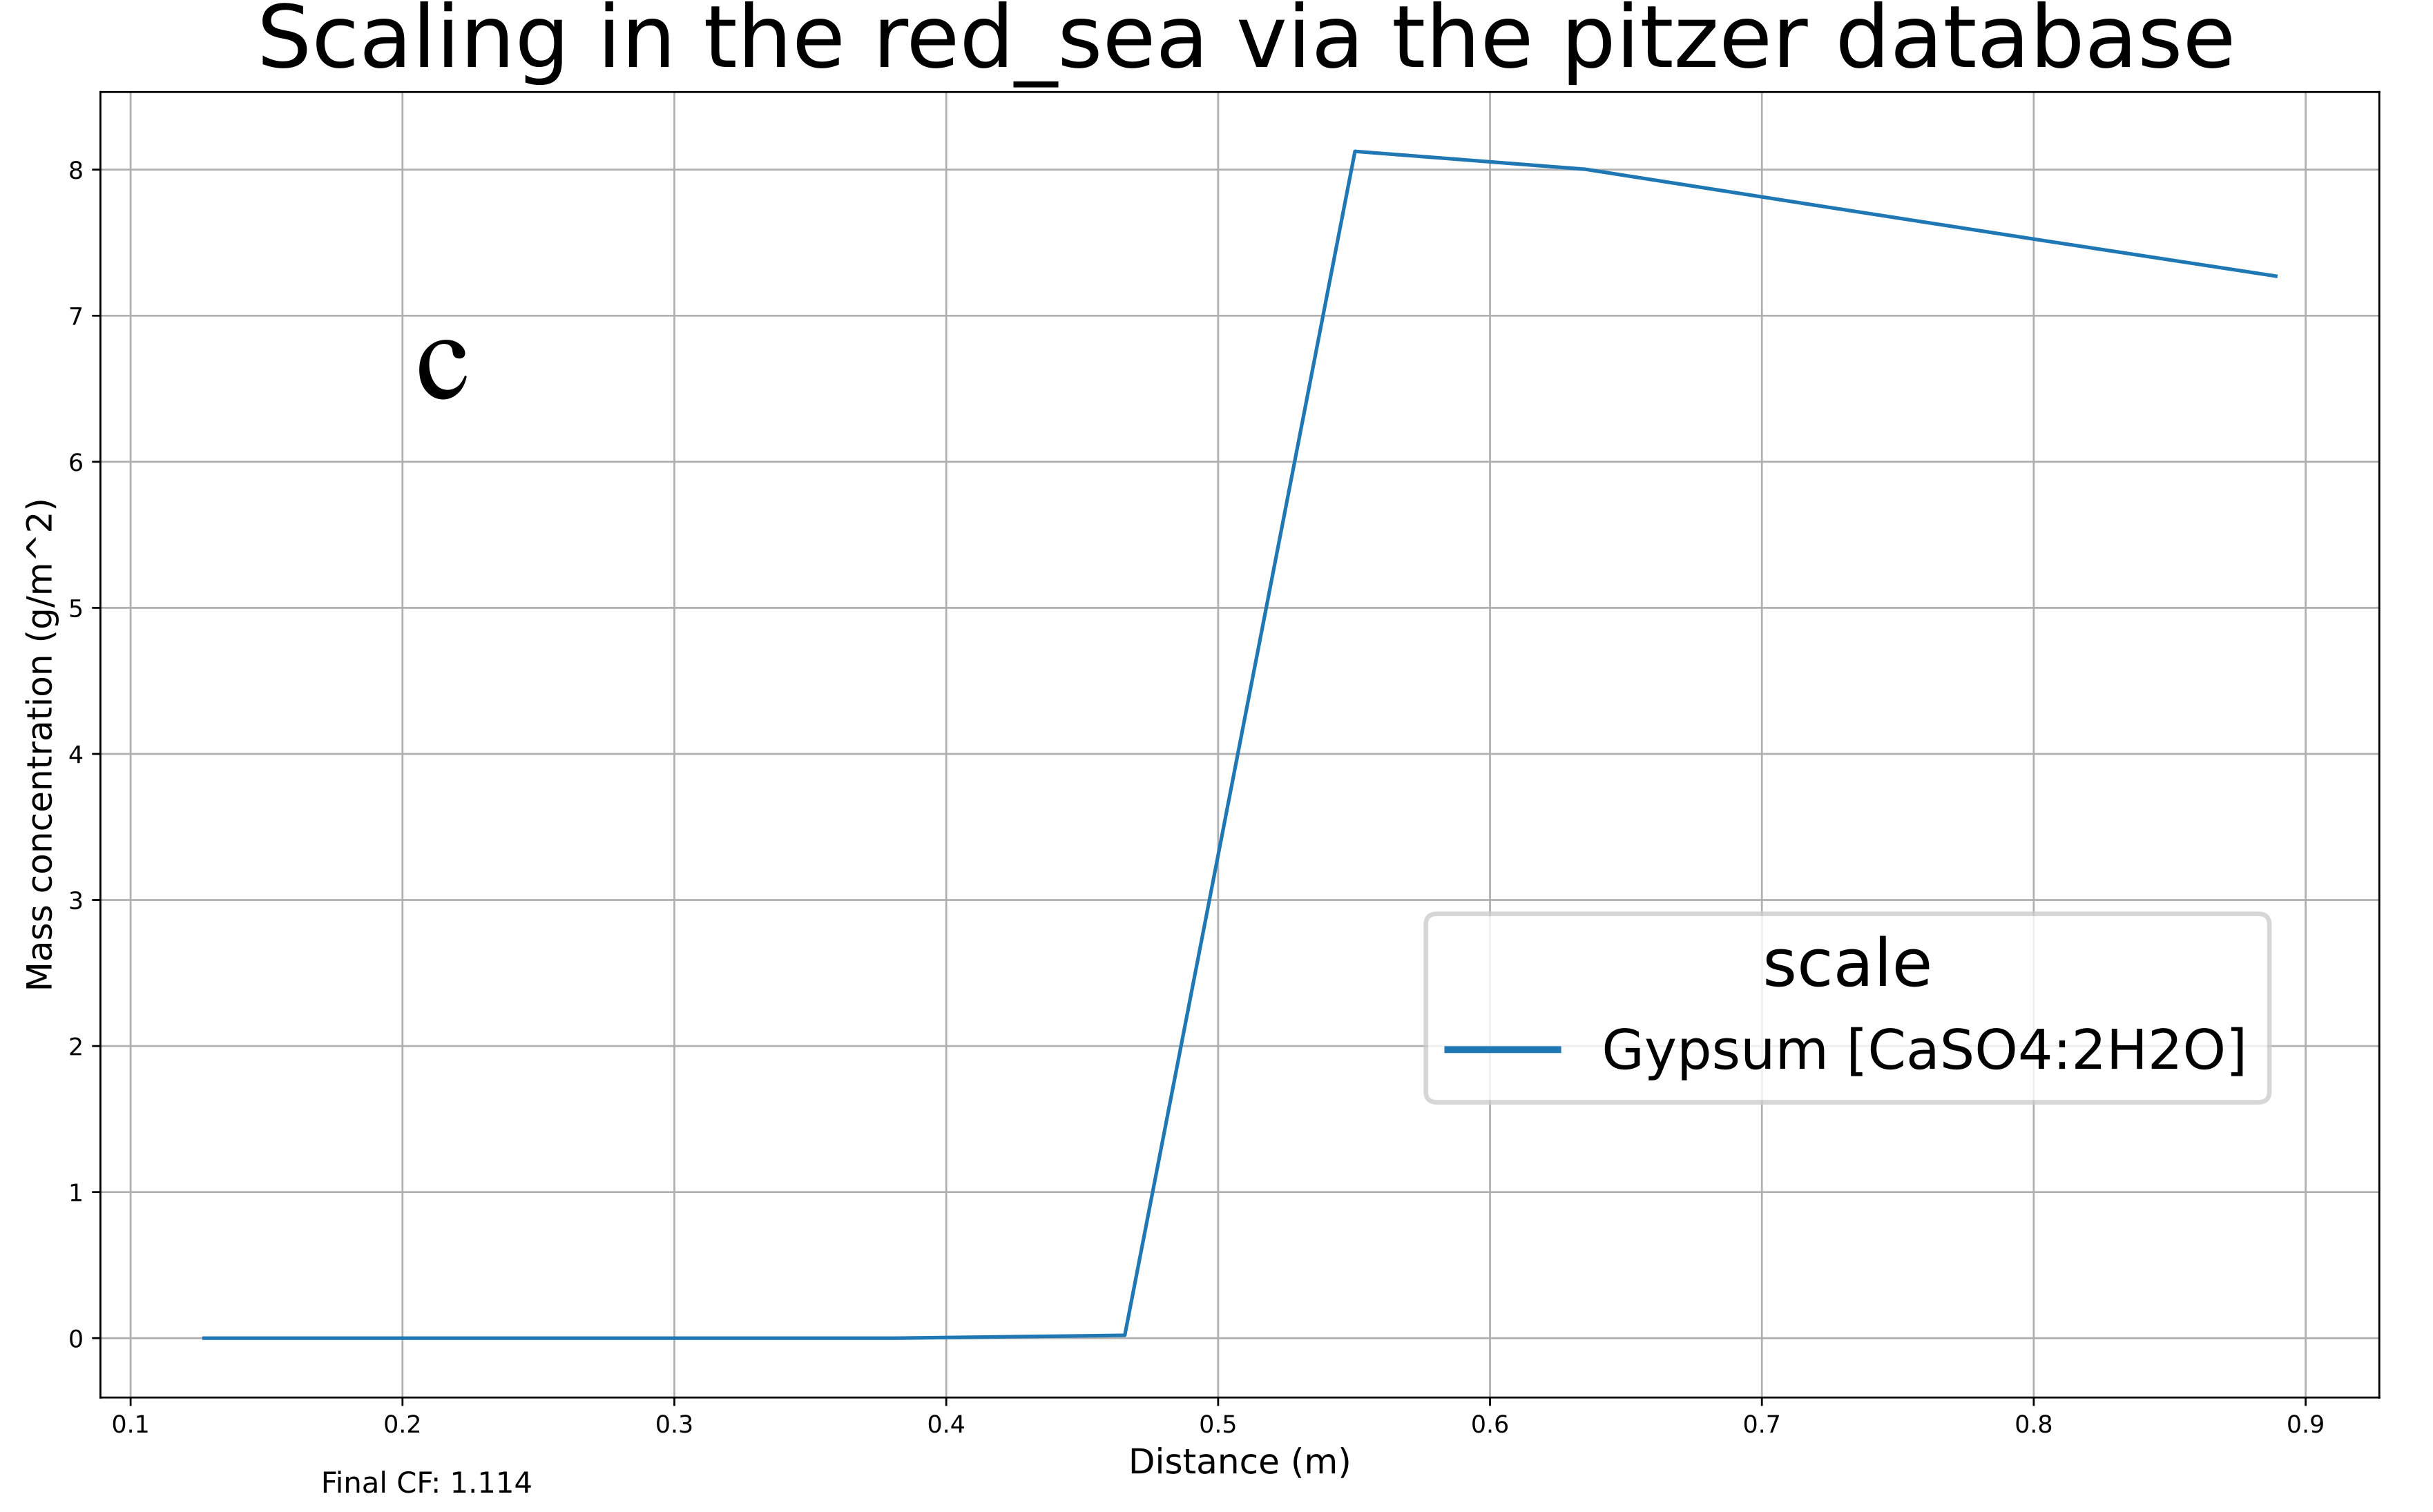
\includegraphics[width=0.49\textwidth]{images/ROSSpy/sensitivity_analyses/databases/Pitzer.png} 
        & 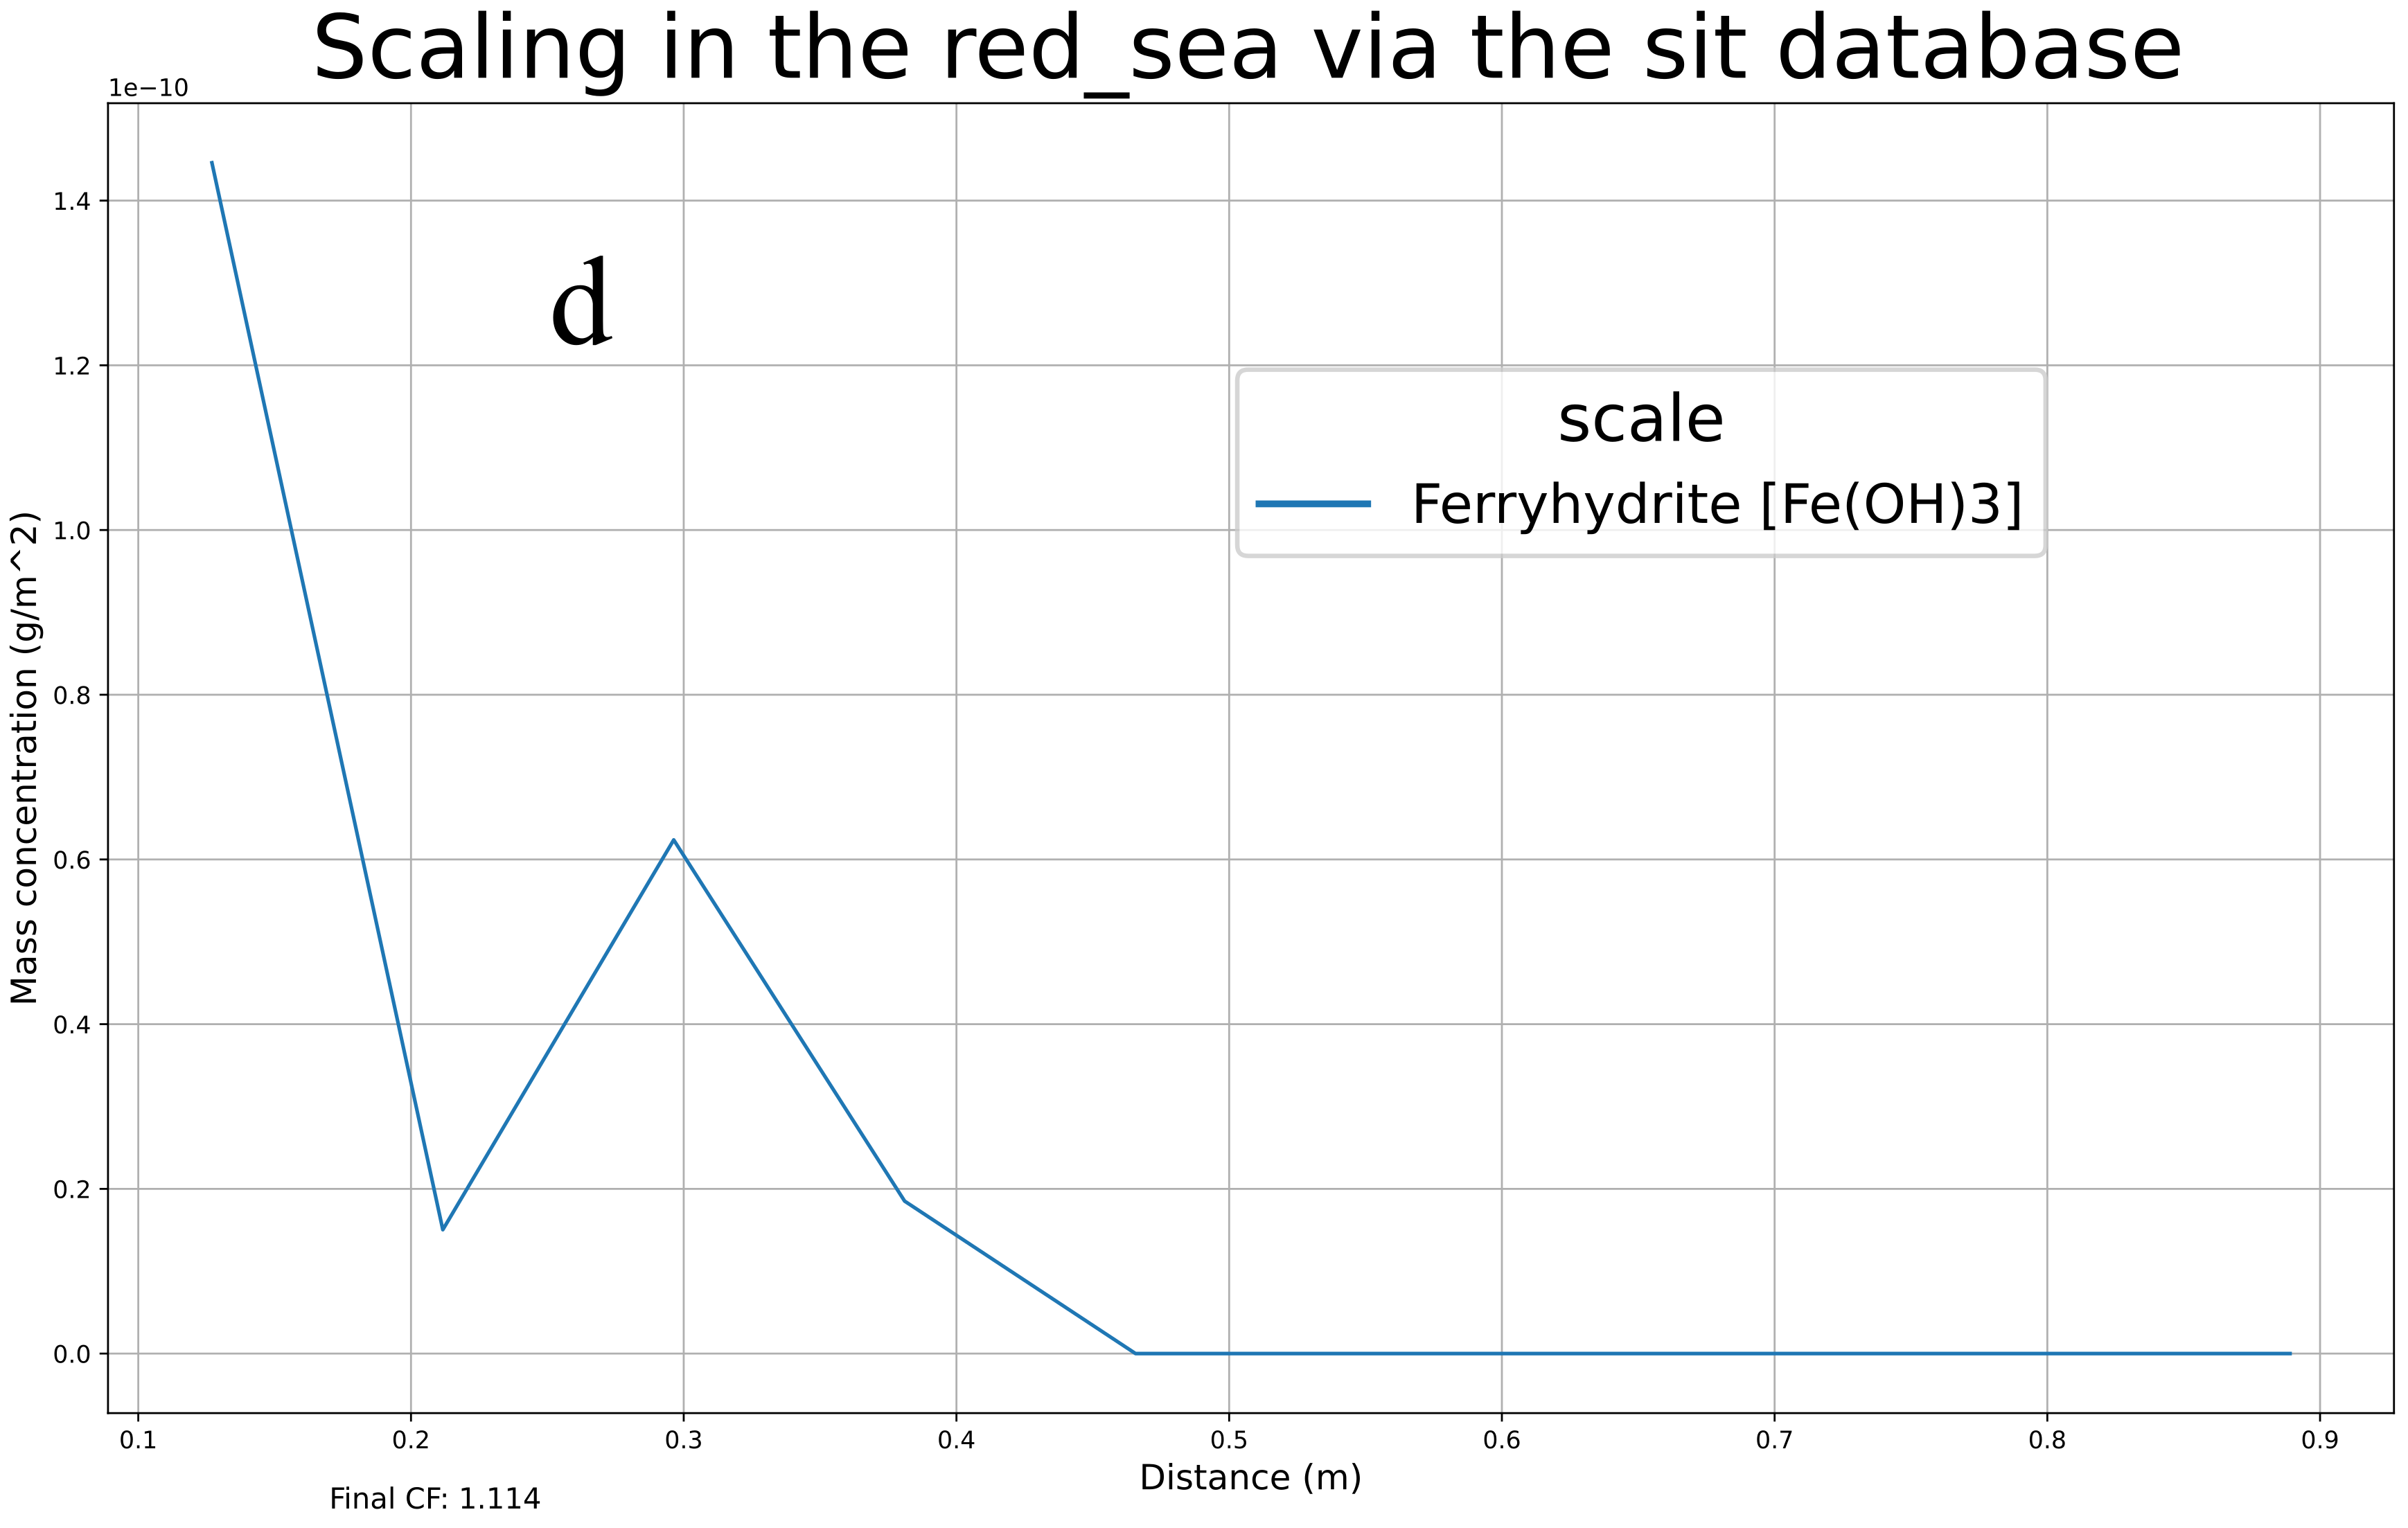
\includegraphics[width=0.49\textwidth]{images/ROSSpy/sensitivity_analyses/databases/Sit.png} 
        \\ \bottomrule
    \end{tabular}
    \caption{
        Scaling predictions from the a) ColdChem, b) Iso, c) Pitzer, and d) Sit databases, with otherwise identical simulation parameters. These subfigures represent the spectrum of similar yet distinct predictions of scaling during the database sensitivity analysis, and exemplify that the PHREEQC database should be deliberately selected after reviewing the PHREEQC documentation to discern which database is most appropriate for the feed geochemistry.
    }
    \label{database_selection}
\end{figure}

\subsection{Feed geochemistry}
The default feed waters were constructed from experimental geochemical literature into parameter files that are provided with ROSSpy. Users of ROSSpy are encouraged to simulate their own feed water while emulating the syntax of the default parameter files. We propose experimental data of numerous other water sources in Section 5 of the Supporting Information that can predicate feed water files; although, direct measurement of the simulated feed water is preferable to avoid significant influences of anthropogenic pollution \cite{Chen2008SourcesSea} and seasonality \cite{Sarthou2001SeasonalSea} in reported measurements. Thee default water sources, which include both natural seas and produced waters from oil wells, were contrasted in Figure \ref{feed_sources}, where the scaling and brine predictions differed significantly amongst these feed water sources. 

\begin{figure}
    \centering
    \begin{tabular}{c|c}
        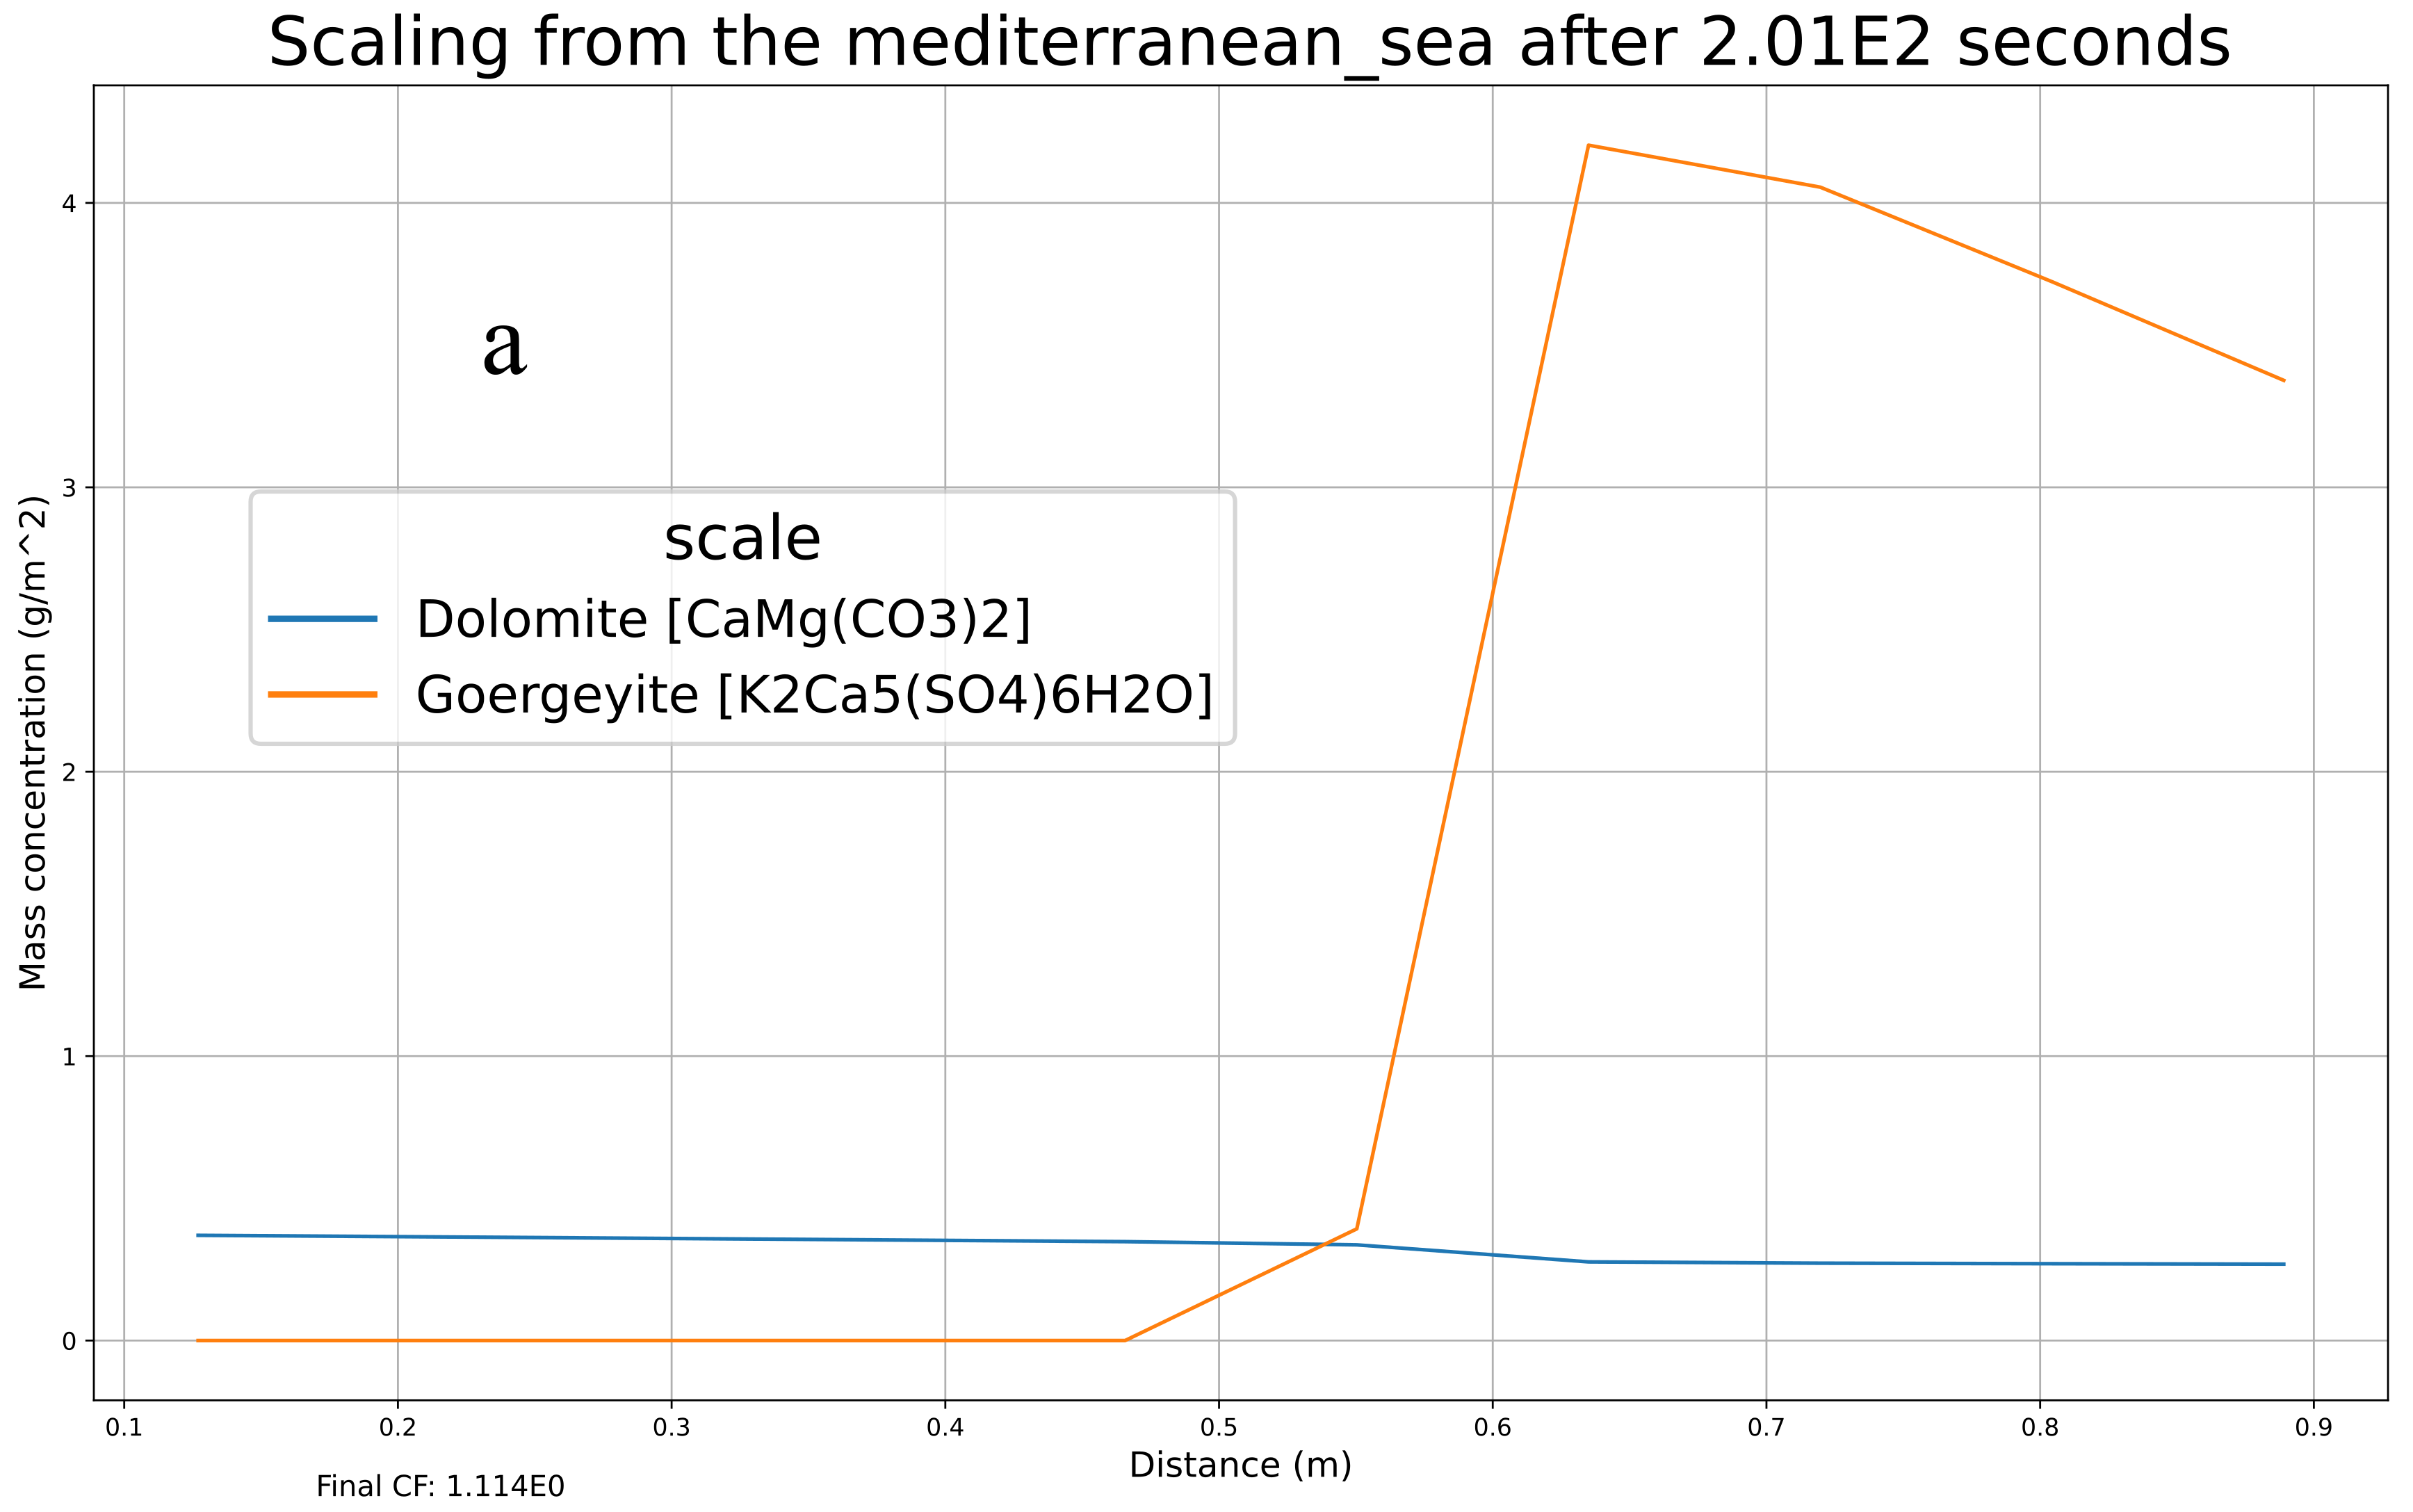
\includegraphics[width=0.49\textwidth]{images/ROSSpy/sensitivity_analyses/feed_source/Mediterranean.png} &
        \includegraphics[width=0.49\textwidth]{images/ROSSpy/sensitivity_analyses/feed_source/Palo_Duro_basin.png} \\ \midrule
        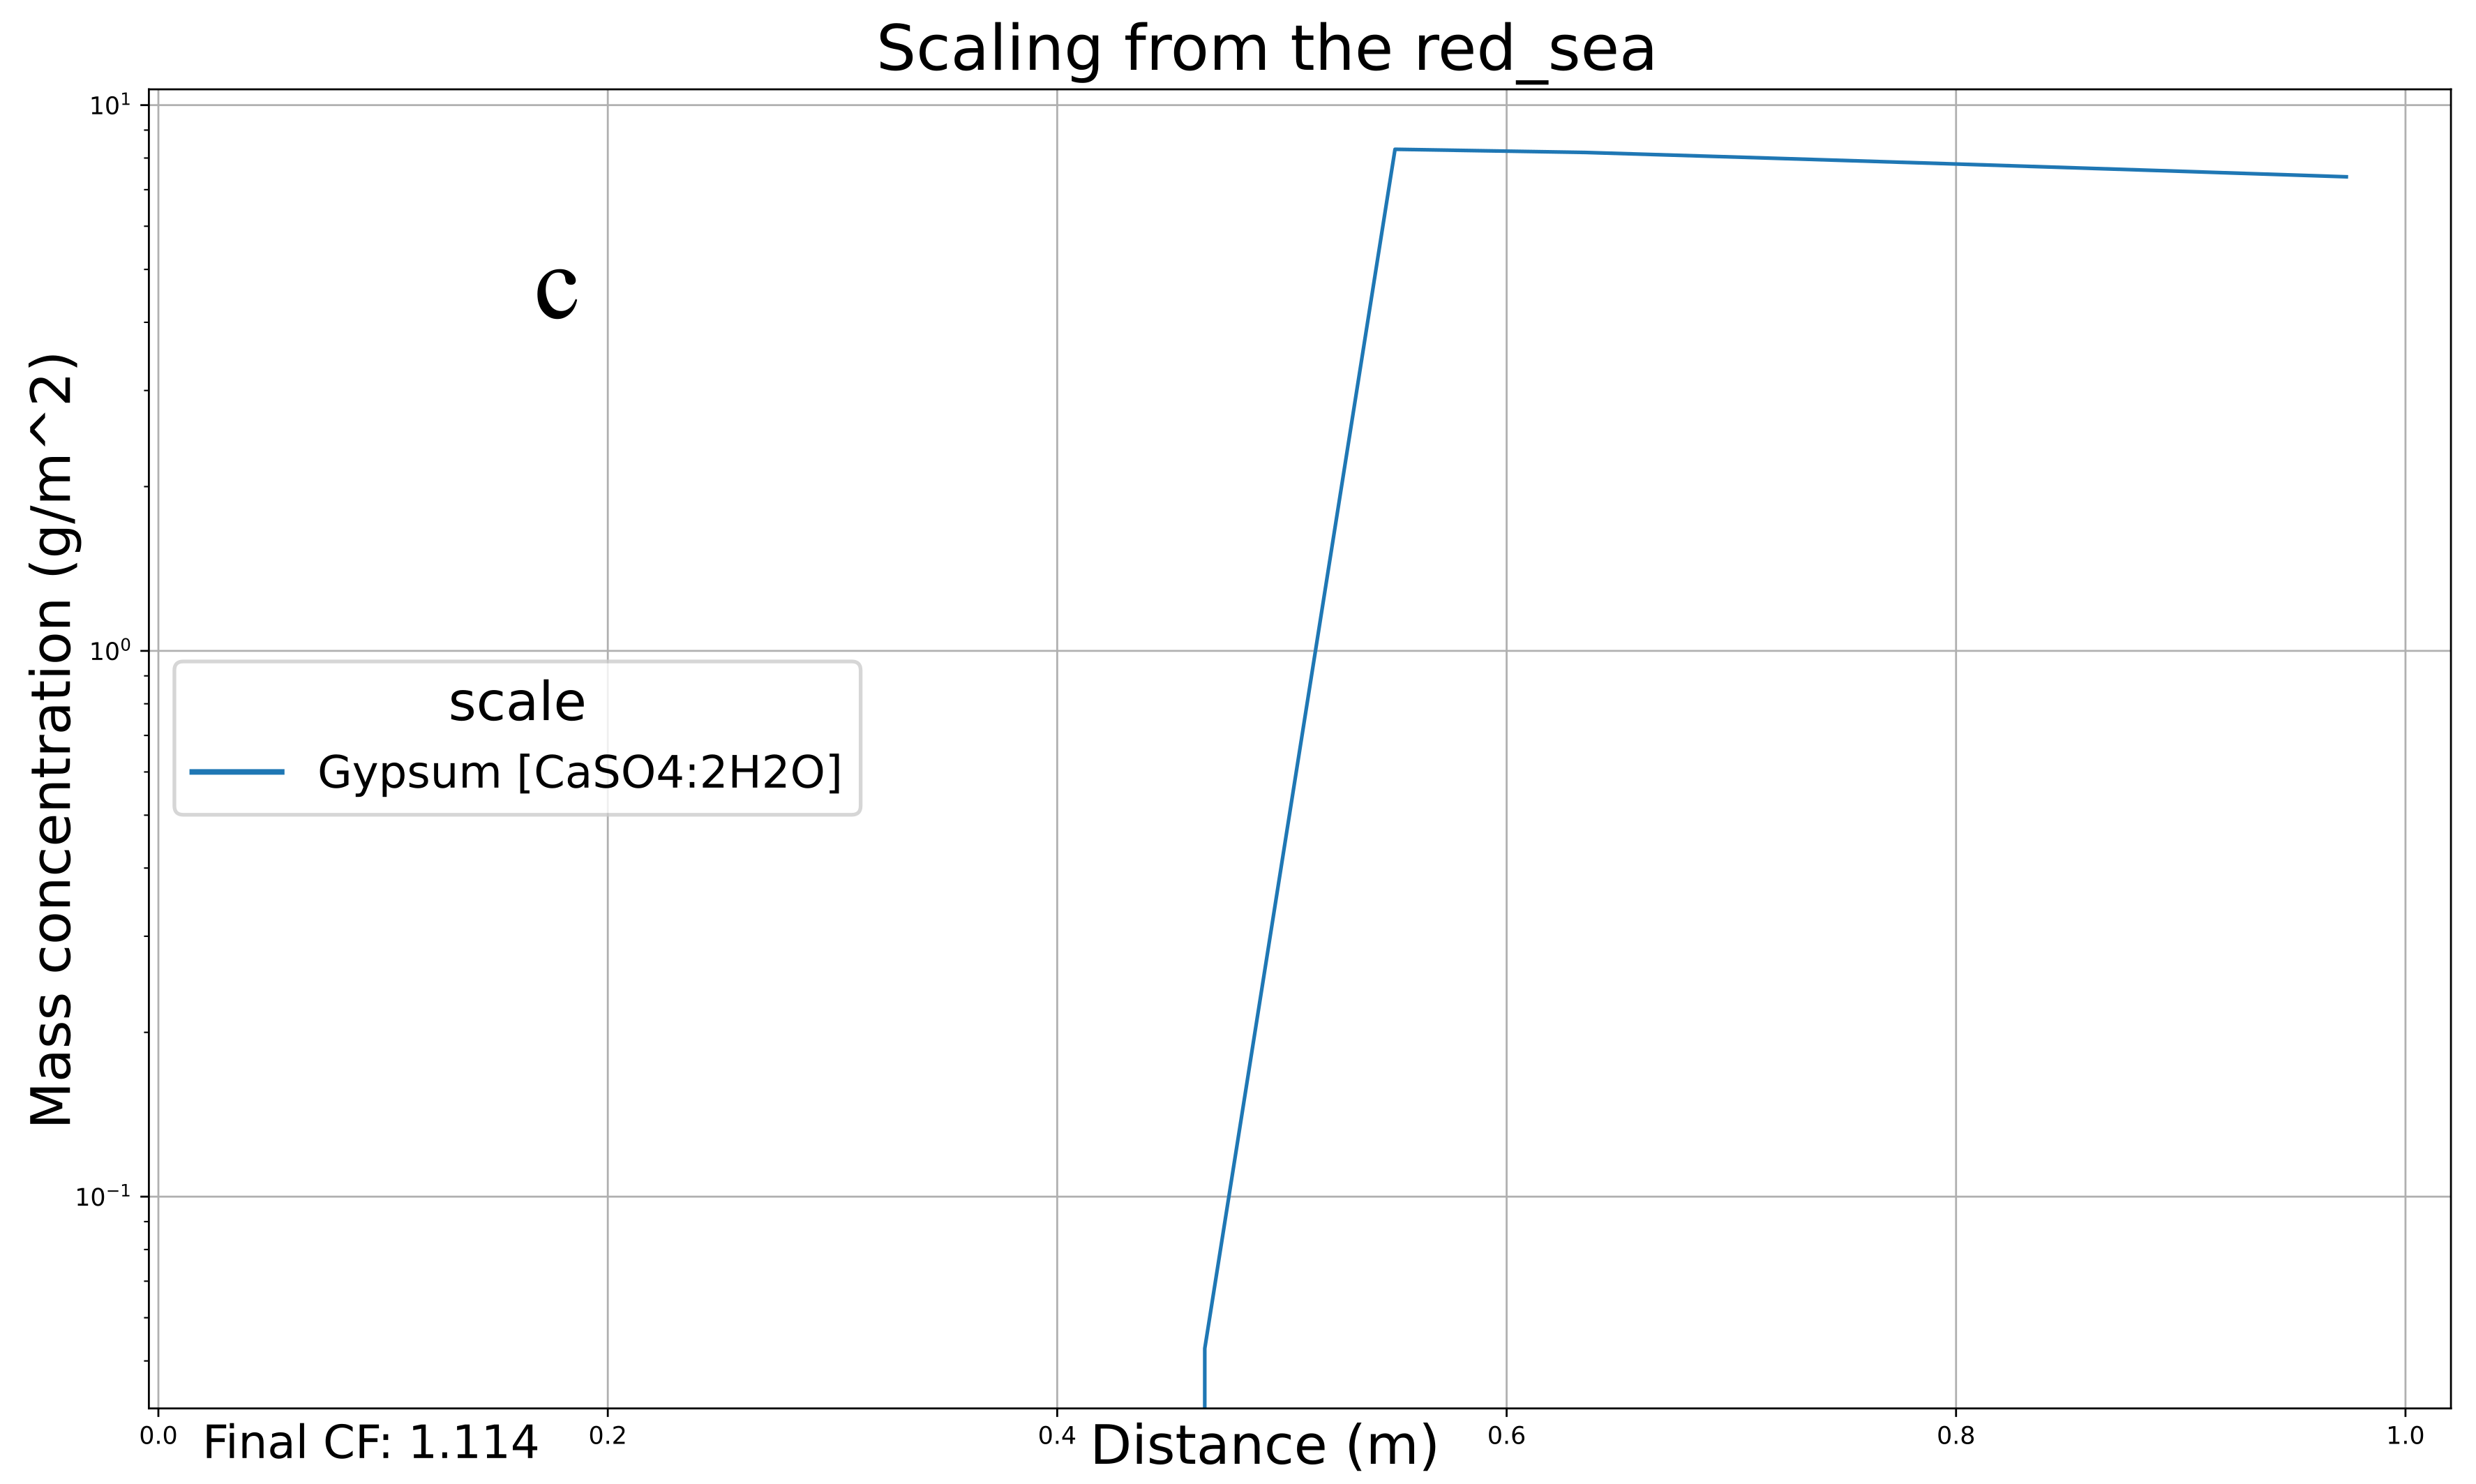
\includegraphics[width=0.49\textwidth]{images/ROSSpy/sensitivity_analyses/feed_source/Red_Sea.png} & 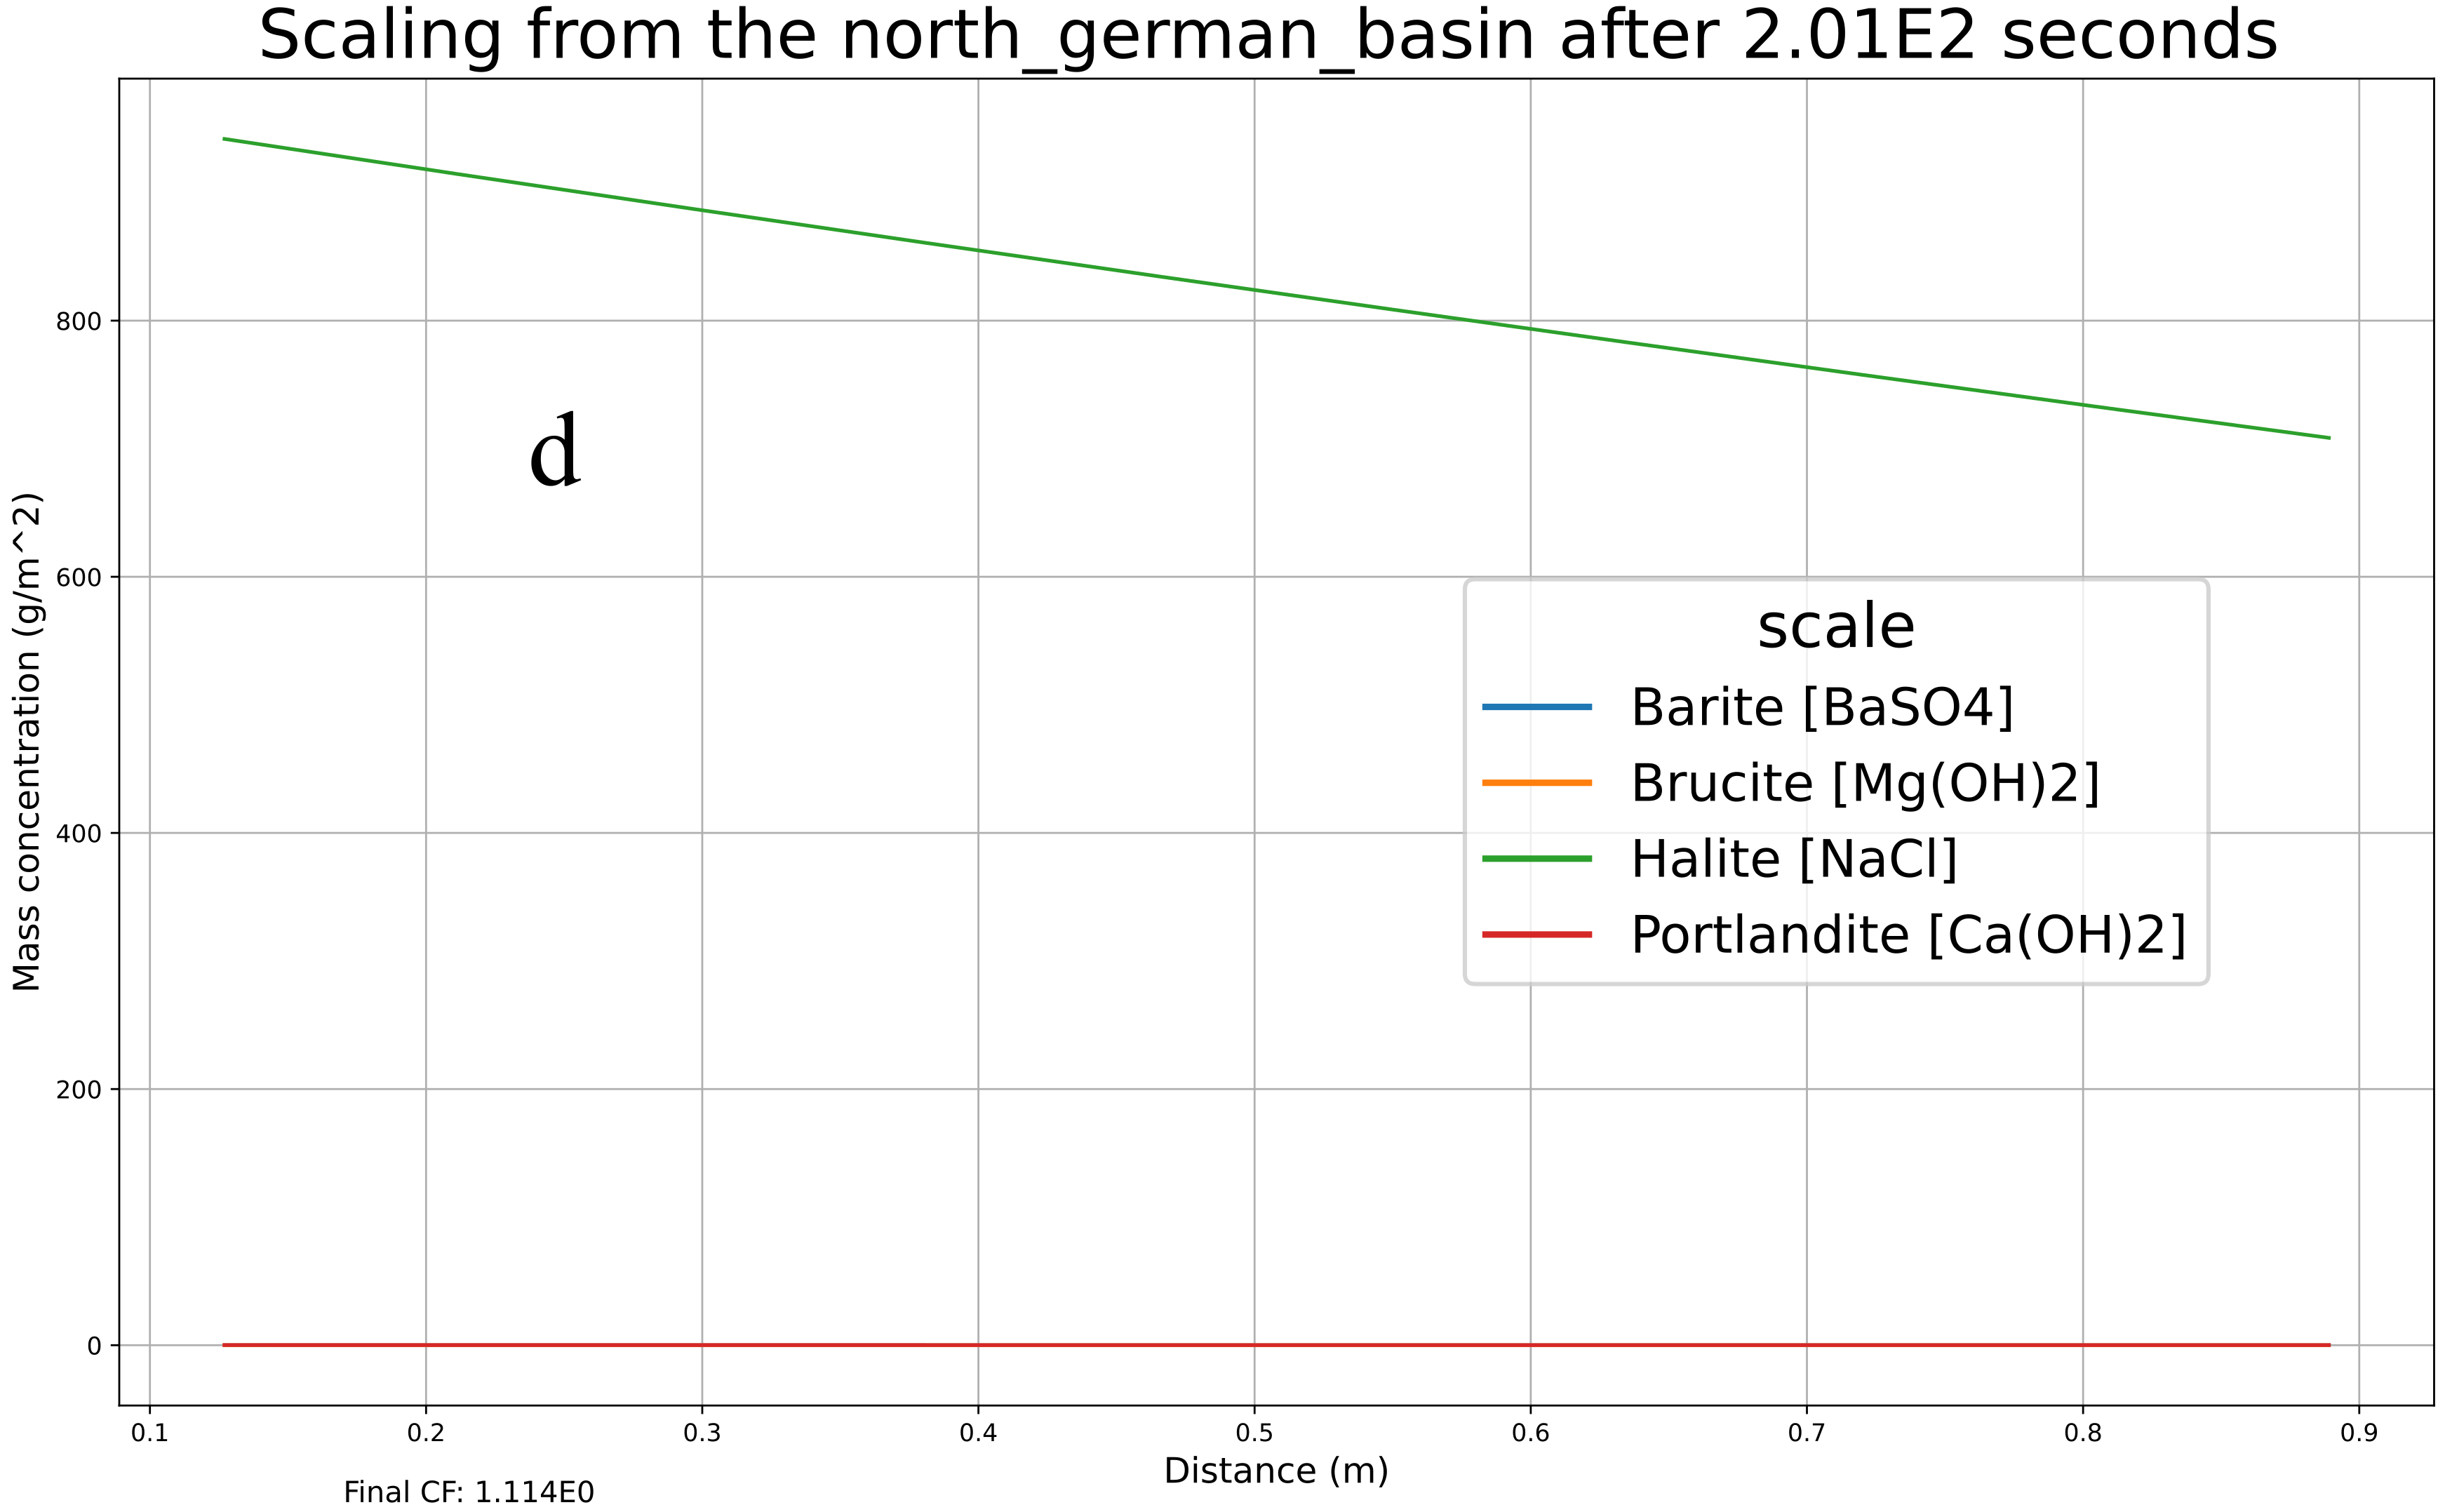
\includegraphics[width=0.49\textwidth]{images/ROSSpy/sensitivity_analyses/feed_source/German_Basin.png} \\ \bottomrule
    \end{tabular}
    \caption{
        Scaling predictions of a) the Mediterranean Sea, b) produced waters from the Palo Duro oil basin, c) the Red Sea, d) produced waters from the North German oil basin, with otherwise identical simulation parameters. These subfigures represent the spectrum of scaling predictions from the variety of different feed sources, which exhibits a high sensitivity of scale predictions to the feed geochemistry. 
    }
    \label{feed_sources}
\end{figure}

\section{Software}
ROSSpy, which is conceptualized by Figure \ref{workflow}, combines our one-dimensional RO model with post-processing operations that facilitate interpretation of the simulation results. The software a) translates parameters into a PHREEQ input file; b) executes that input file via PHREEQpy; c) processes the simulation results into figures and data tables via Matplotlib \cite{Hunter2007Matplotlib:Environment} and Pandas \cite{McKinney2011Pandas:Statistics} Python packages, respectively; and d) exports all of the simulation content -- e.g. the PHREEQ input file, SVG data figures, and CSV files of parameters, variables, data, and brine predictions -- into a specified folder and directory. The simulation data may be sliced into one-dimensional sets of distance or time that can be plotted against either scaling density or brine concentrations (Figures S2-S3) (see ROSSpy documentation).


\begin{figure}
    \centering
    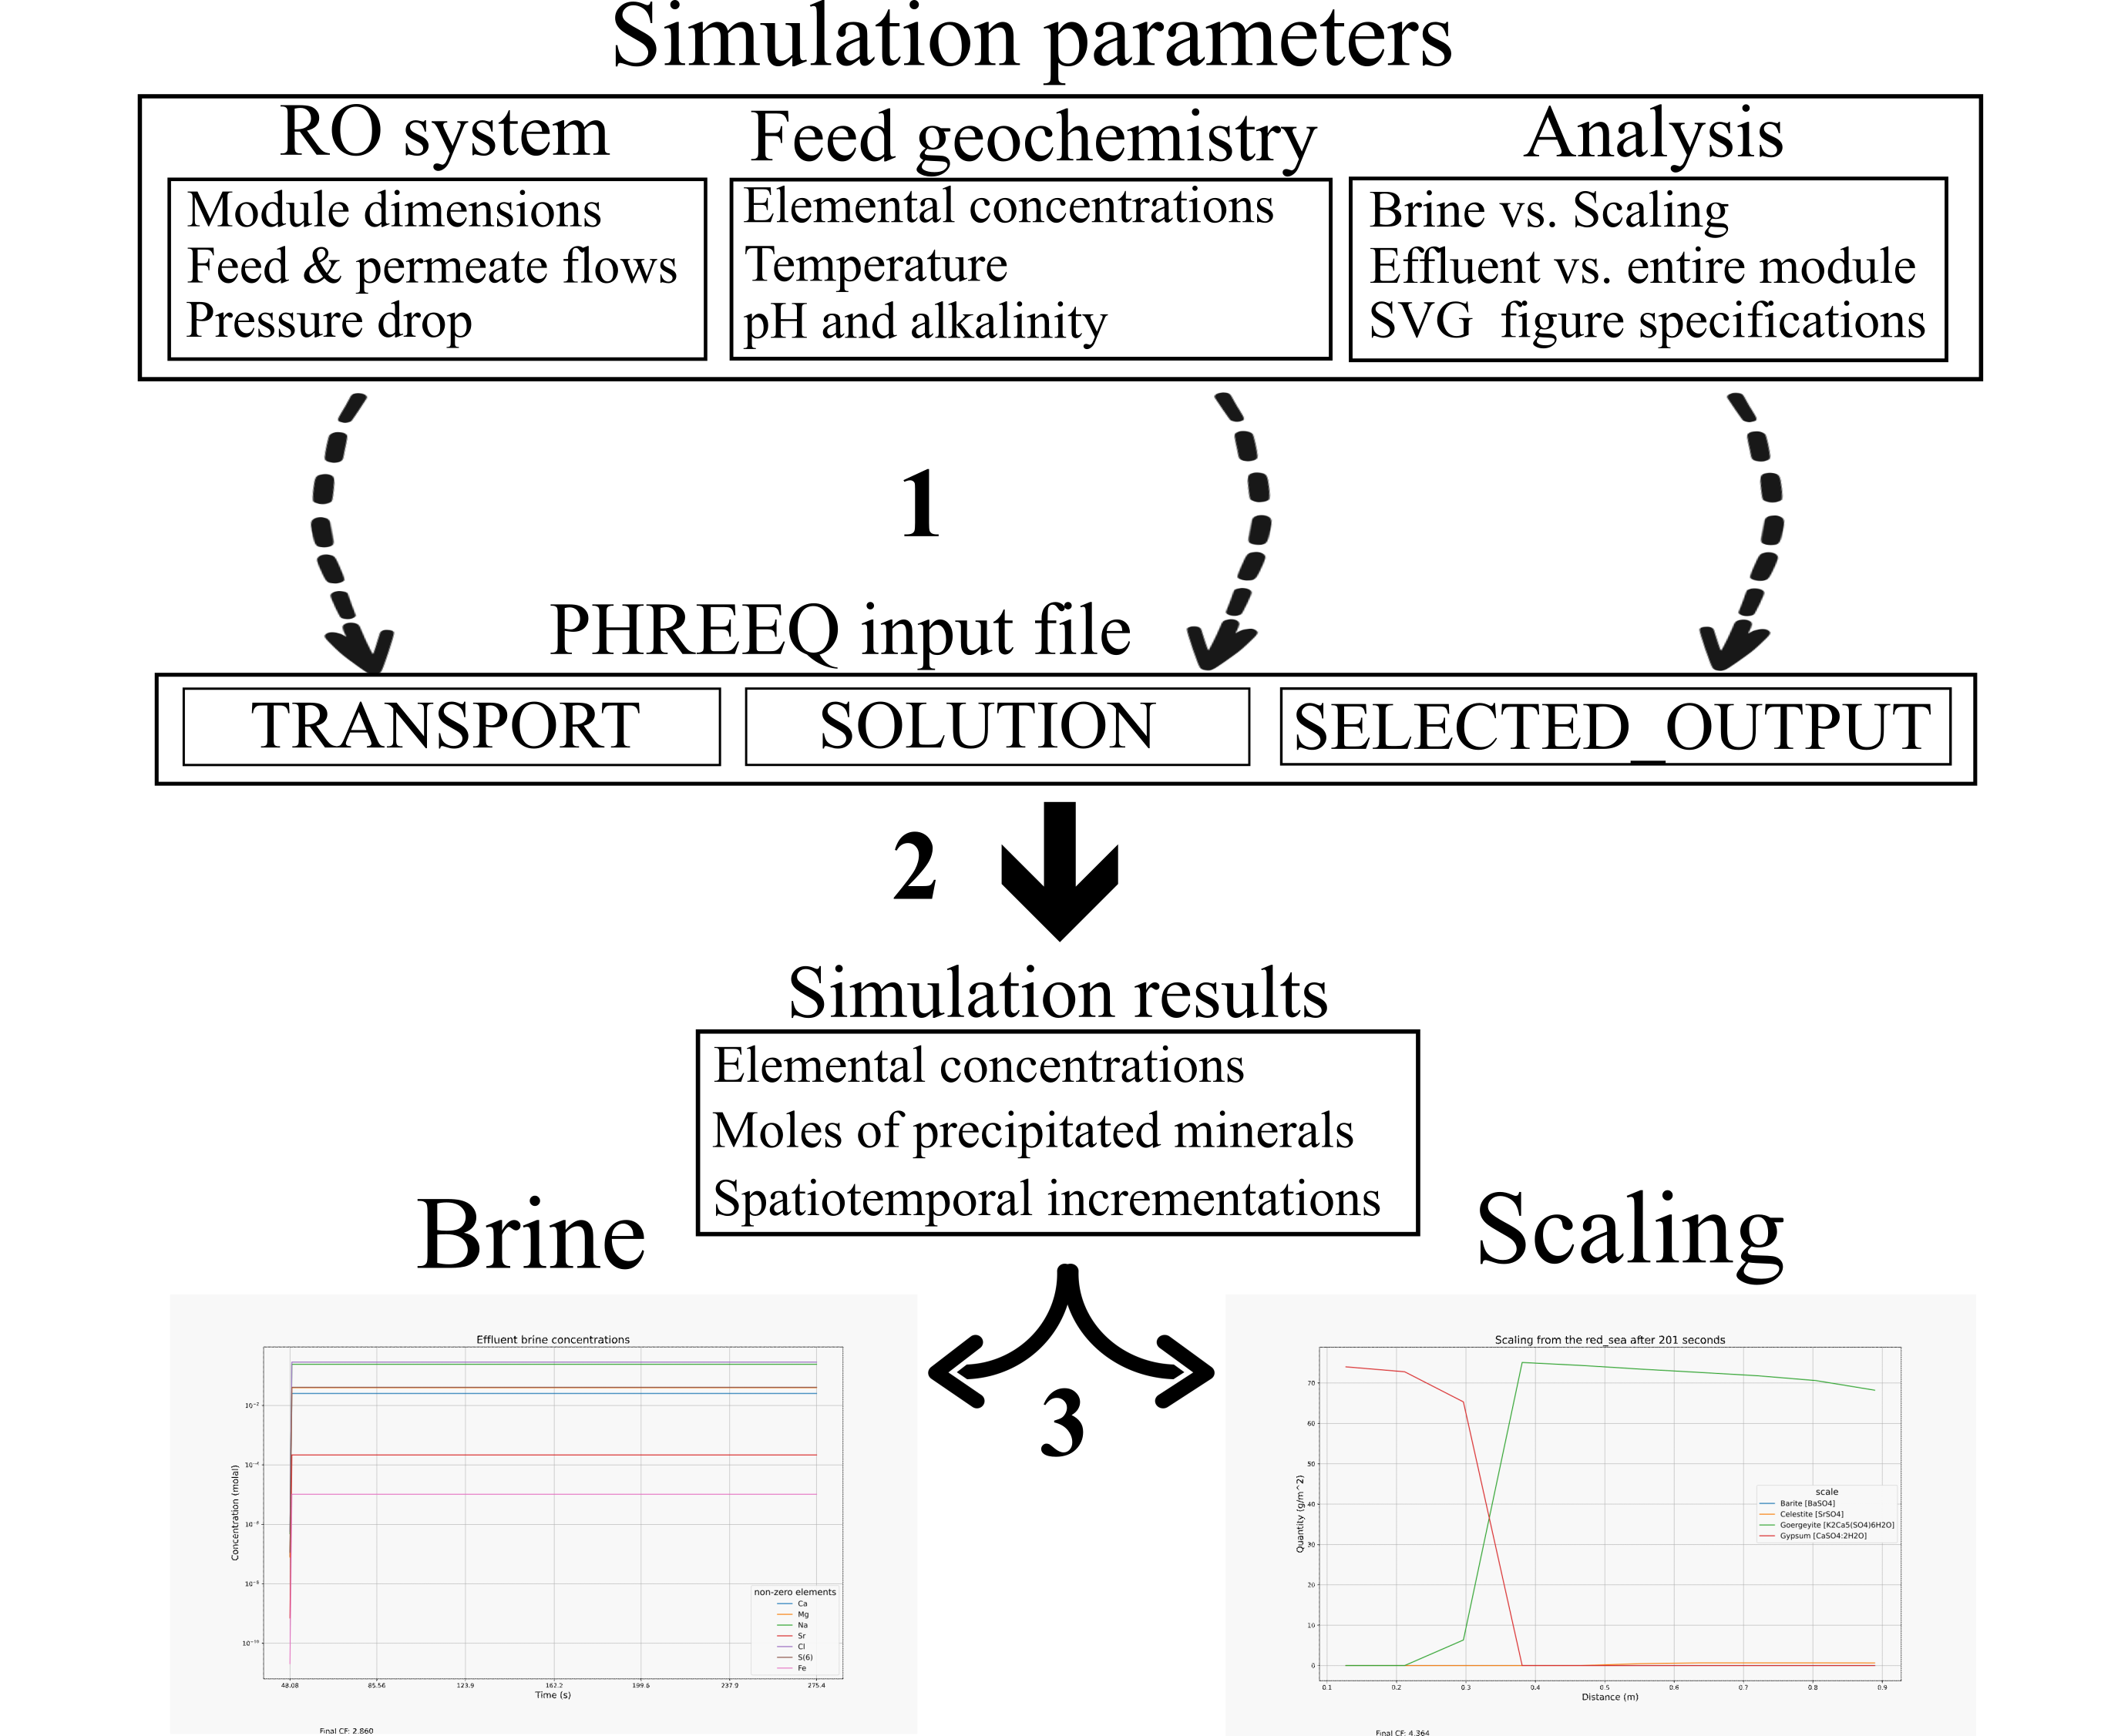
\includegraphics[width = \linewidth]{images/ROSSpy/rosspy_workflow_1.PNG}
    \caption{
        The ROSSpy workflow. Step 1 describes the translation of parameters -- i.e. module specifications, feed geochemistry, and simulation analysis -- into the corresponding code blocks of a PHREEQ input file. Step 2 describes executing the PHREEQ input file via either PHREEQpy in ROSSpy, or via the PHREEQC batch software in the interactive version of ROSSpy (iROSSpy) that is under development. Step 3 describes processing the predictions of brine concentrations or scaling quantities into representative figures and datatables, which are ultimately exported.
    }
    \label{workflow}
\end{figure}

\section{Conclusion}

A one-dimensional approximation of RO reactive transport geochemistry, executed in PHREEQC, is a practical and accurate representation of mineral scaling during desalination. The simulation predictions of this model were quantitatively and qualitatively verified for a few use cases, with both theoretical expectations and experimental data where it was available. The API implementation of this model (ROSSpy) furthermore meets identified needs of the community -- e.g. rapidly designing, executing, processing, and exporting simulations of RO scaling -- while maintaining accessibility through its light-weight design and its open-source code. We expect that this one-dimensional model and the unique attributes of ROSSpy  will facilitate scaling research and ultimately improve the efficiency of RO desalination towards alleviating chronic water insecurities in the world. 

\section{Funding}
This work was prepared in partial fulfillment of the requirements of the Berkeley Lab Undergraduate Research (BLUR) Program, managed by Workforce Development \& Education at the Berkeley Lab. The project was also partly funded by NSERC Discovery, MITACS Accelerate, CEWIL, and Canada Summer Jobs. 

% Acknowledgements section
\section{Acknowledgement}
The authors thank Ethan Sean Chan for his technical assistance in developing a graphical interface of ROSSpy (iROSSpy) that will be released in a future version. 
\newpage


% \layout
%     \setlength{\hoffset}{0pt}
%     \setlength{\voffset}{0pt}
%     \setlength{\topmargin}{0pt}
%     \setlength{\oddsidemargin}{0pt}
%     \setlength{\marginparwidth}{0pt}
%     \setlength{\marginparsep}{0pt}
%     \setlength{\textwidth}{465pt}
%     \setlength{\textheight}{600pt}
% \layout*


\section{Supporting Information}

\begin{supplementary}

\subsection{ROSSpy}

The variables and terms that comprise our model are defined in Table \ref{glossary}.

\begin{longtable}{c|c|c}
    \caption{
        Glossary of ROSSpy variables.  
        \label{glossary} 
    } \\ \toprule
    
    \textbf{variable} & \textbf{name} & \textbf{description} \\ \toprule
    \endfirsthead
    \multicolumn{3}{c}{continuation of Table \ref{glossary}} \\  \toprule
    \textbf{variable} & \textbf{name} & \textbf{description} \\ \toprule
    \endhead
    
    \multirow{2}{1.5em}{$l$} & \multirow{2}{3em}{length} & longitudinal dimension of the\\& & module or module cell \\ \midrule
    \multirow{2}{1.5em}{$n$} & number of & quantity of discretizations of the module \\ & module cells & \\ \midrule
    $\Phi_e$ & moles & the $moles_{H_2O}$ that exist in cell $e$ \\ \midrule  
    $\Delta \Phi_e$ & permeate flux & the $moles_{H_2O}$ that are removed in cell $e$ \\ \midrule  
    $HL$ & head loss & reduction of pressure over the module distance \\ \midrule
    \multirow{2}{2em}{$PE$} & \multirow{2}{3em}{permeate efficiecy} & attenuation of permeate flux \\& & from pre-existing inefficiencies \\ \midrule  
    \multirow{2}{2em}{$CF$} & \multirow{2}{3em}{concentration factor} & solution concentration of cell $e$ normalized \\& & to the influent concentration \\ \midrule
    $X$ & mass & water mass in the maximally filled feed channel \\ \midrule
    $V$ & velocity & feed velocity through the feed channel \\ \midrule
    $A$ & area & cross-sectional area of the RO module \\ \midrule
    $th$ & thickness & thickness of a module dimension \\ \midrule
    $Q$ & volumetric flow & feed flow through a maximally filled feed channel \\ \midrule
    \multirow{2}{1.5em}{$\Delta t$} & \multirow{2}{3em}{time} & timestep of the simulation that \\& & adheres to the Courant condition \\ \midrule
    \multirow{2}{2em}{$C_{max}$} & \multirow{2}{3em}{Courant constant} & maximal value of the Courant constant \\& & to meet the Courant condition \\ \midrule
    $\phi$ & total concentration & total ionic concentrations in the simulation \\ \midrule
    $C$ & specie concentration & concentration of an individual specie \\ \midrule
    \multirow{2}{1em}{$v$} & \multirow{2}{3em}{stoichiometry coefficient} & coefficient for the respective compound \\& & in the balanced equilibrium reaction \\ \midrule
    \multirow{2}{1em}{$N$} & number of & quantity of reactions that \\& reactions & contain a respective compound \\ \midrule
    $R$ & reaction flux & $\frac{mmol}{hour}$ flux of an equilibrium reaction \\ \midrule
    \multirow{2}{1em}{$\Omega$} & thermodynamic & logarithm of the $\frac{Q_{dissolution}}{K_{sp}}$ \\& displacement & \\ \midrule
    $k_m$ & rate constant & dissolution and precipitation rate constant \\ \midrule
    $a$ & activity & chemical activity of the respective compound \\ \midrule
    $\eta$ \& $p$ & parameter & experimentally determined parameter \\ \midrule
    \multirow{2}{2em}{$\Delta G$} & \multirow{2}{5em}{Gibbs free energy} & Gibbs free energy of the dissolution \\& & and precipitation reactions \\ \midrule
    $K$ & equilibrium constant & thermodynamic equilibrium of the respective reaction \\ \midrule
    $M$ & number of minerals & quantity of minerals in the studied system \\ \midrule
    $\gamma$ & activity coefficient & coefficient of metabolite activity in a respective system \\ \midrule
    $z$ & charge & compound charge of the respective metabolite \\ \midrule
    $\mu$ & ionic strength & charge-weighted concentration of a solution \\ \midrule
    $A$ \& $B$ & parameter & experimentally determined parameter \\ \midrule
    $a_j$ \& $b_j$ & fitted parameter & geochemical parameter that is fit to the system \\ \midrule
    $W_{aq}$ & water mass & mass of water in the system \\ \bottomrule
\end{longtable} 

The distinctions between slicing the simulation data through time or module distance is exhibited with brine in Figure \ref{brine_perspectives} and scaling in Figure \ref{scaling_perspectives}, respectively.

\begin{figure}
    \centering
    \begin{tabular}{c}
        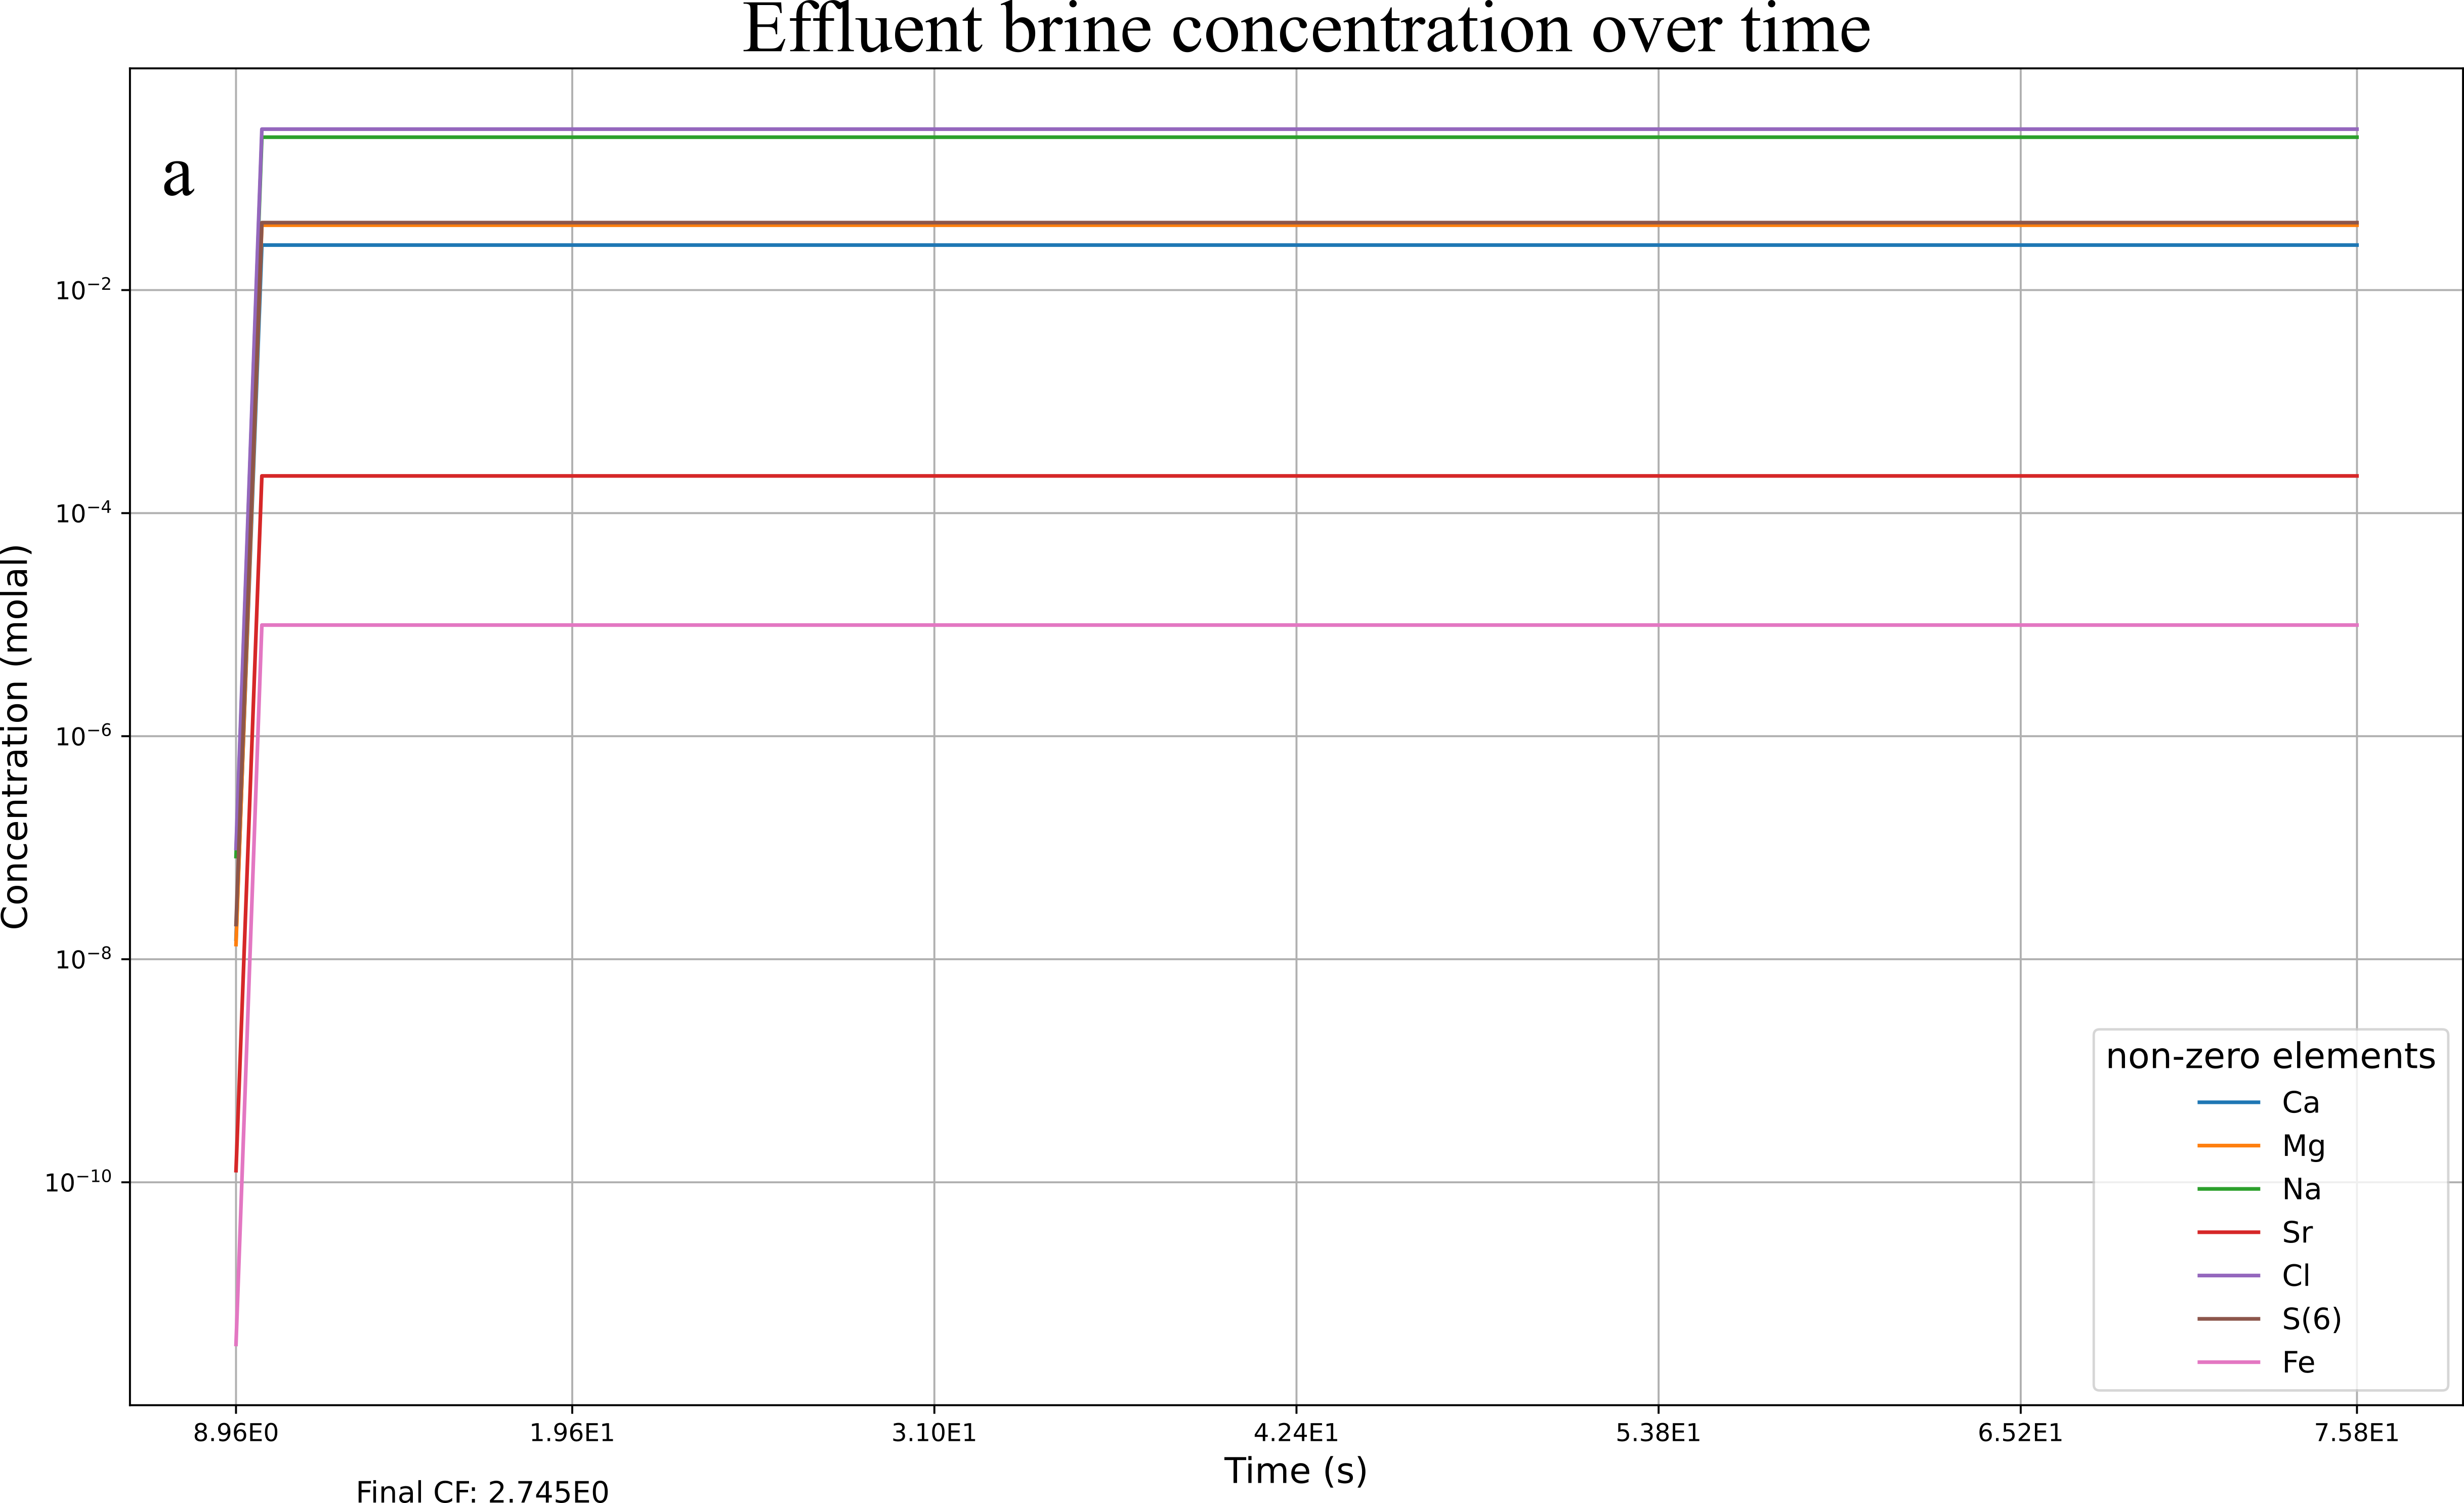
\includegraphics[width=0.8\linewidth]{images/ROSSpy/sensitivity_analyses/simulation_perspective/all_time_brine.png} \\ \midrule
        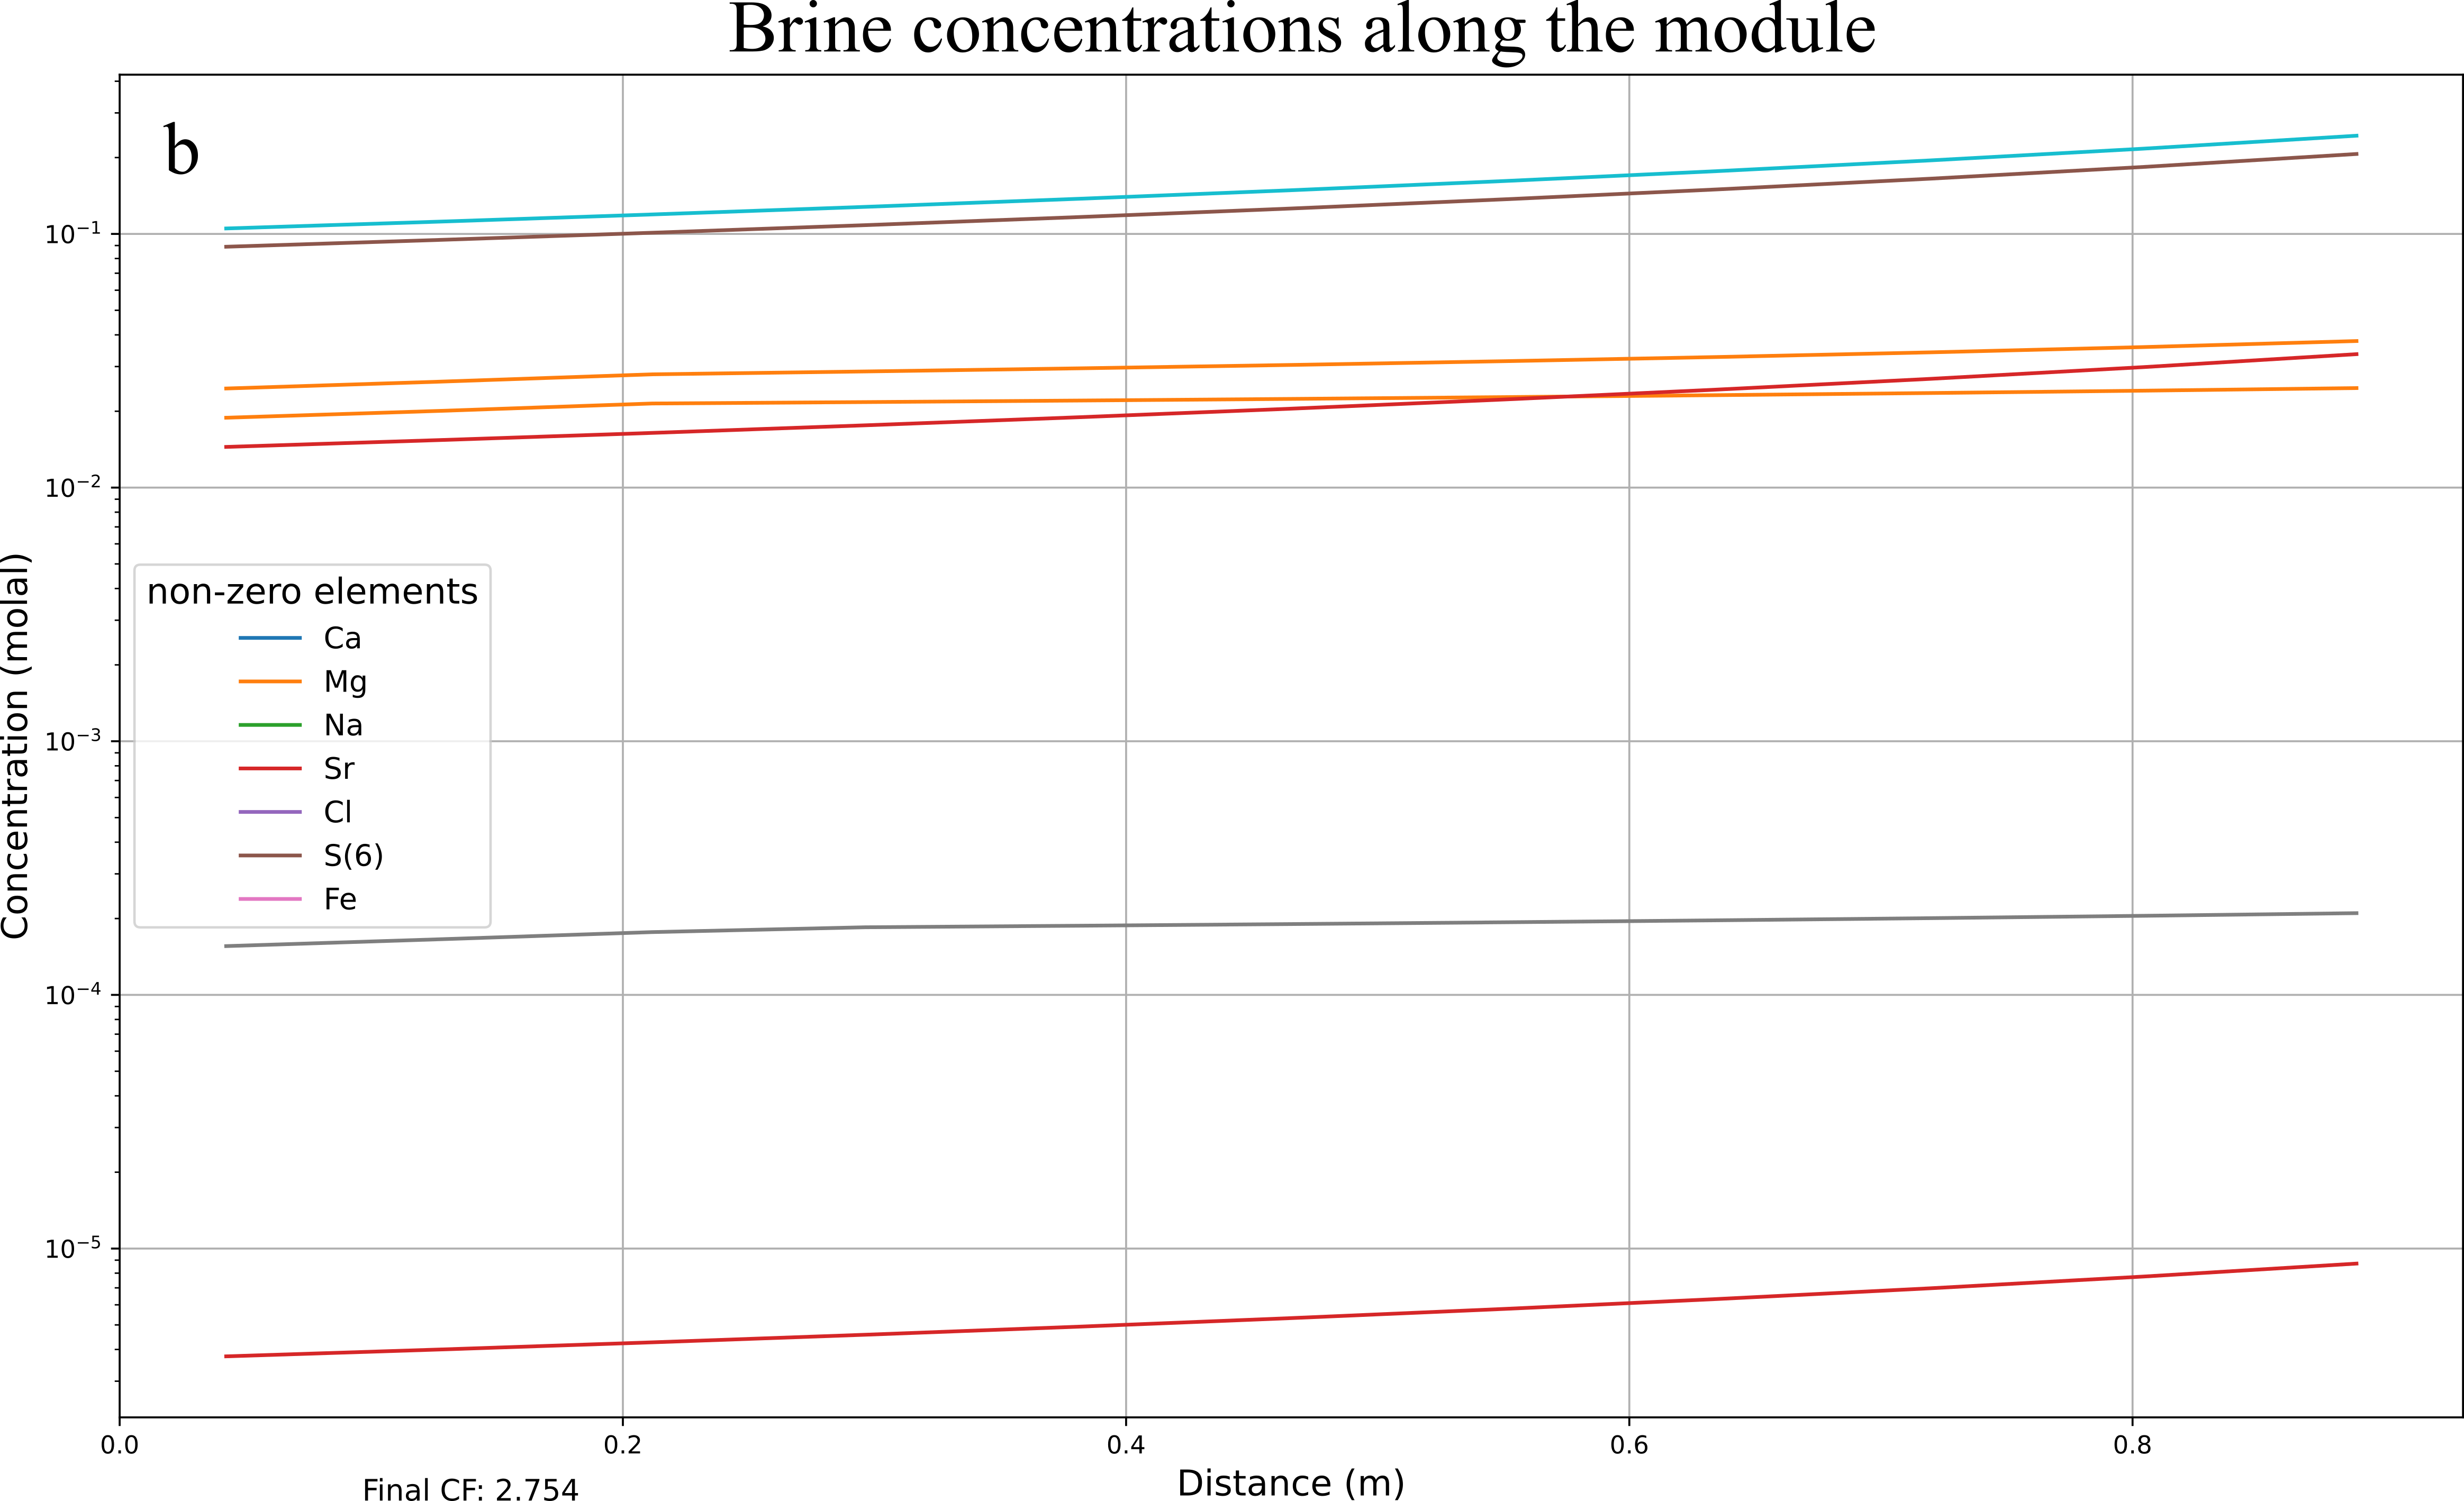
\includegraphics[width=0.8\linewidth]{images/ROSSpy/sensitivity_analyses/simulation_perspective/all_distance_brine.png}
    \end{tabular}
    \caption{
        Brine formation while slicing through either a) time at the final cell or b) distance at the final time. The end concentrations slightly differ between these two simulation perspectives, where the all\_time perspective calculates the true end of the last cell while the all\_distance perspective calculates the mid-point of the last cell and thus has a slightly lower concentration. The brine represents desalination of the Red Sea through the BW30-400 module.
    }
    \label{brine_perspectives}
\end{figure}

\begin{figure}
    \centering
    \begin{tabular}{c}
        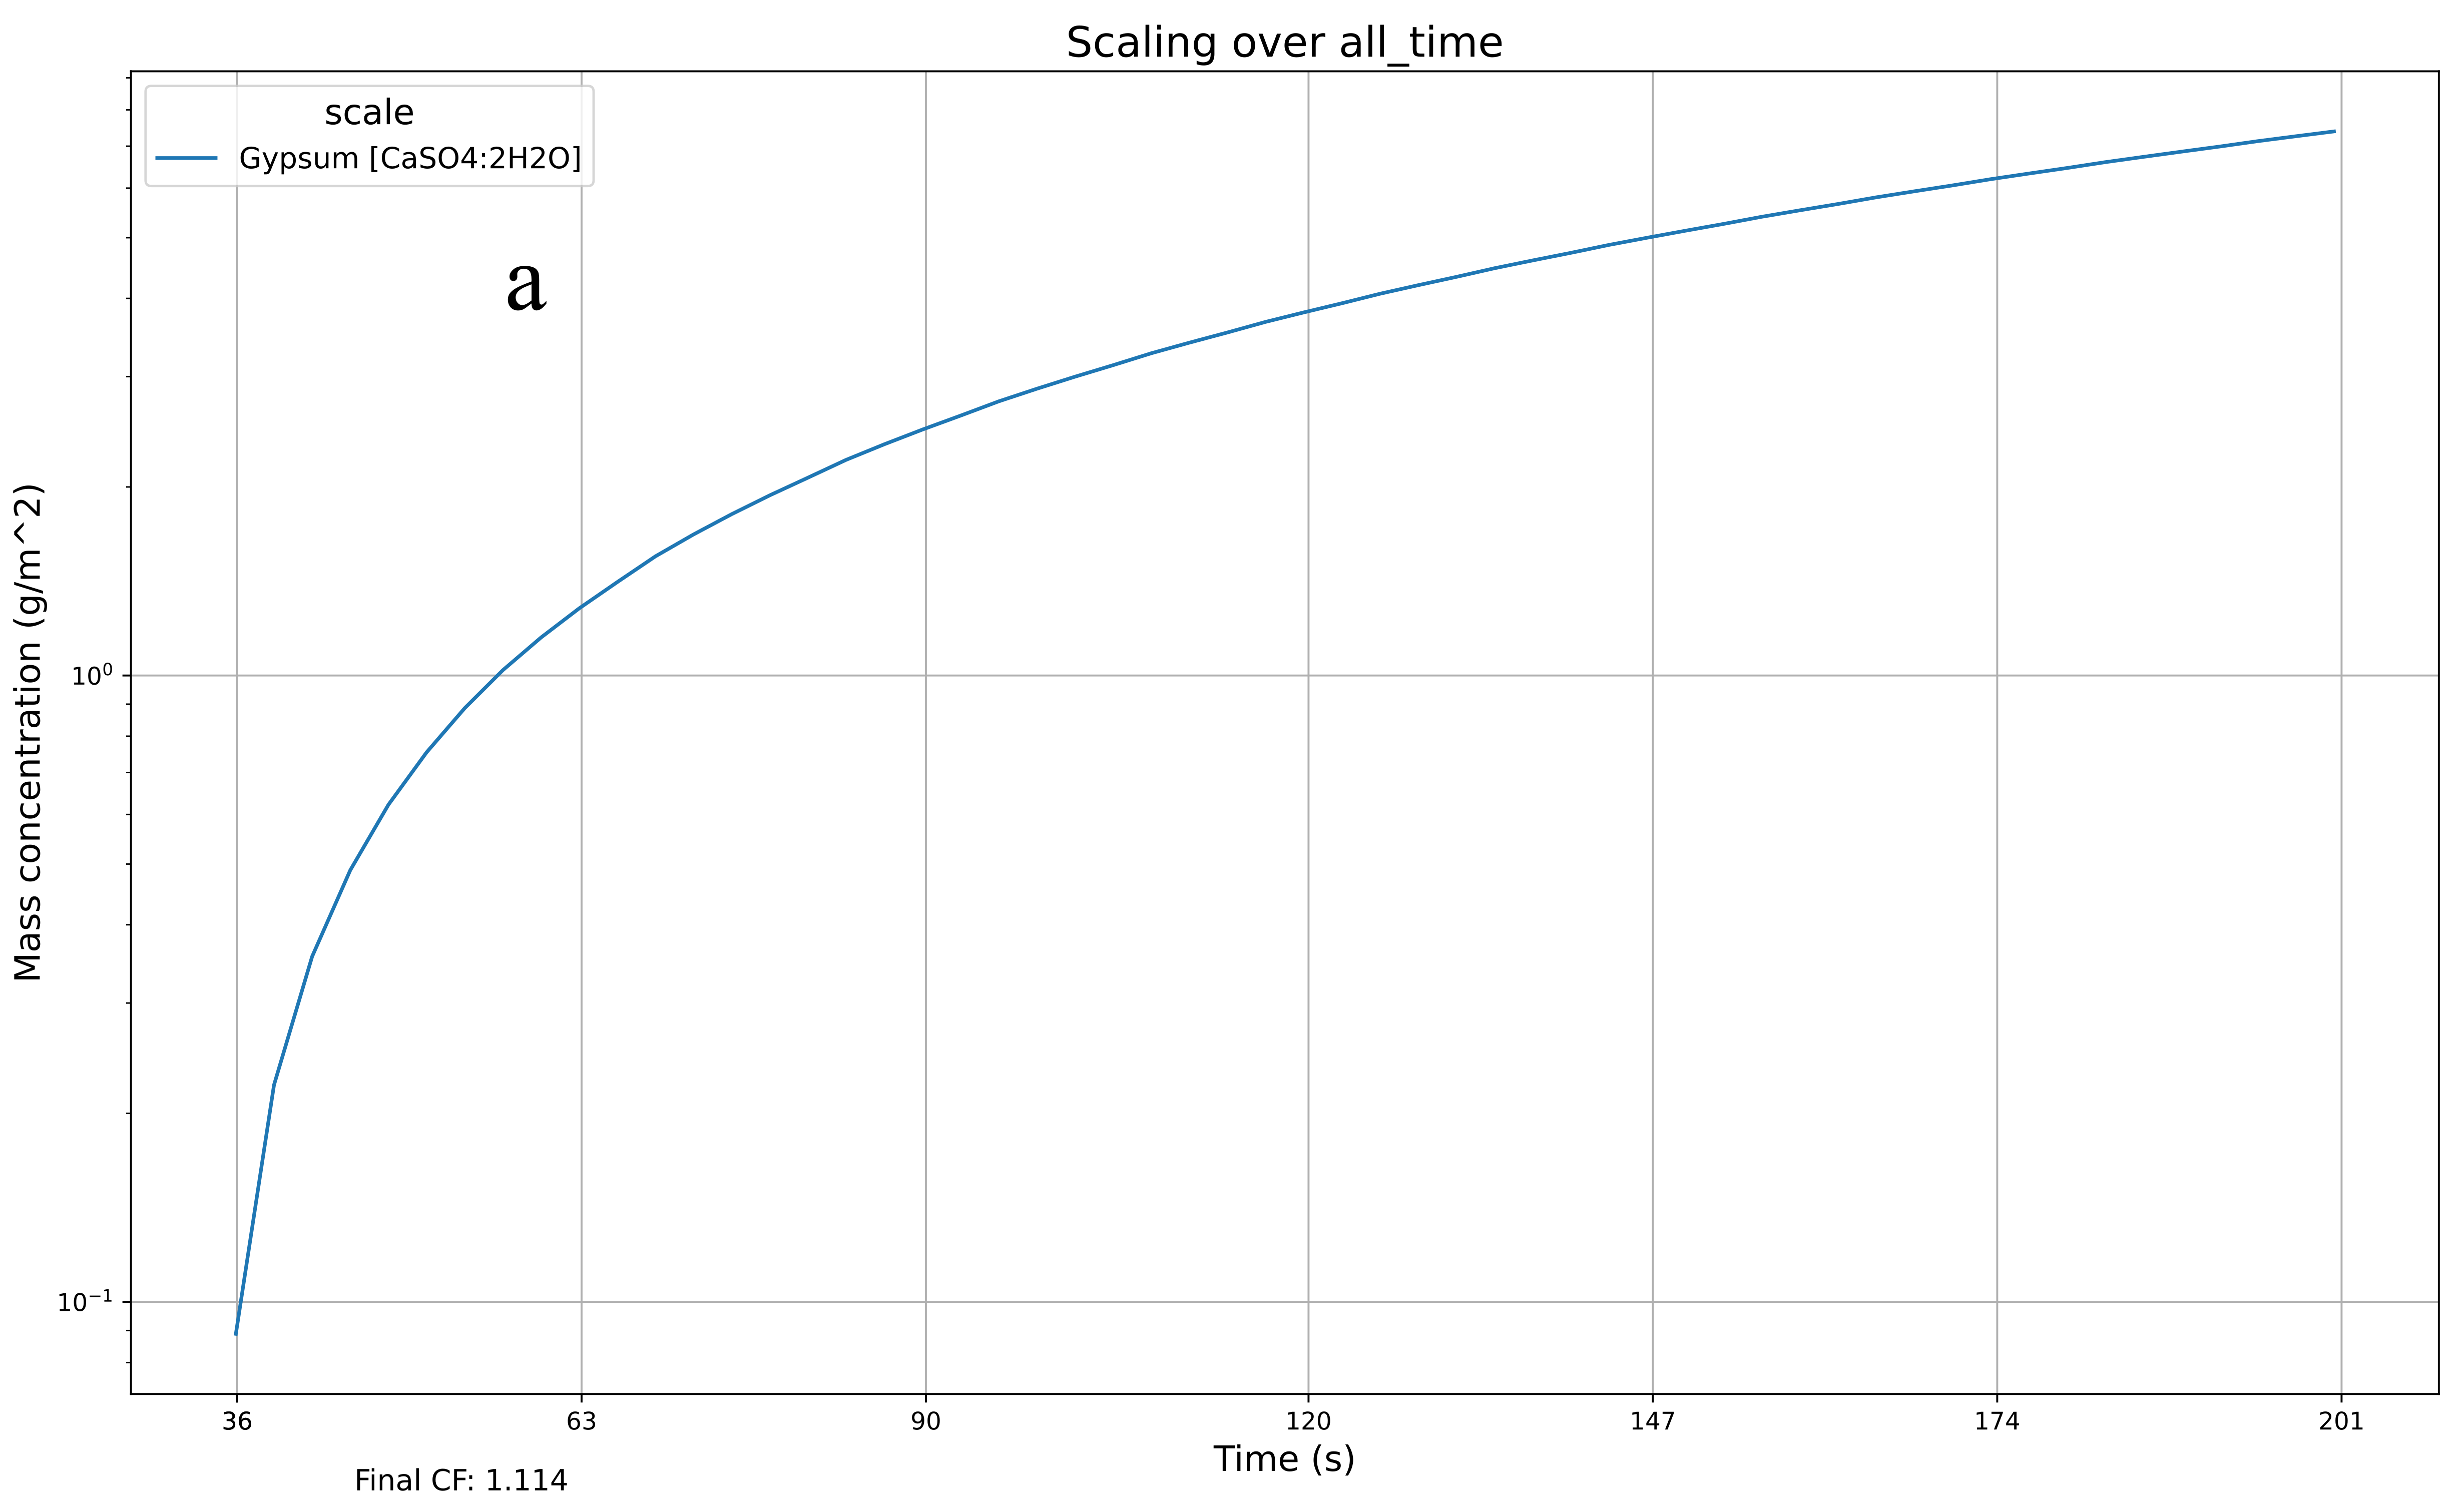
\includegraphics[width=\linewidth]{images/ROSSpy/sensitivity_analyses/simulation_perspective/all_time.png} 
        \\ \midrule
        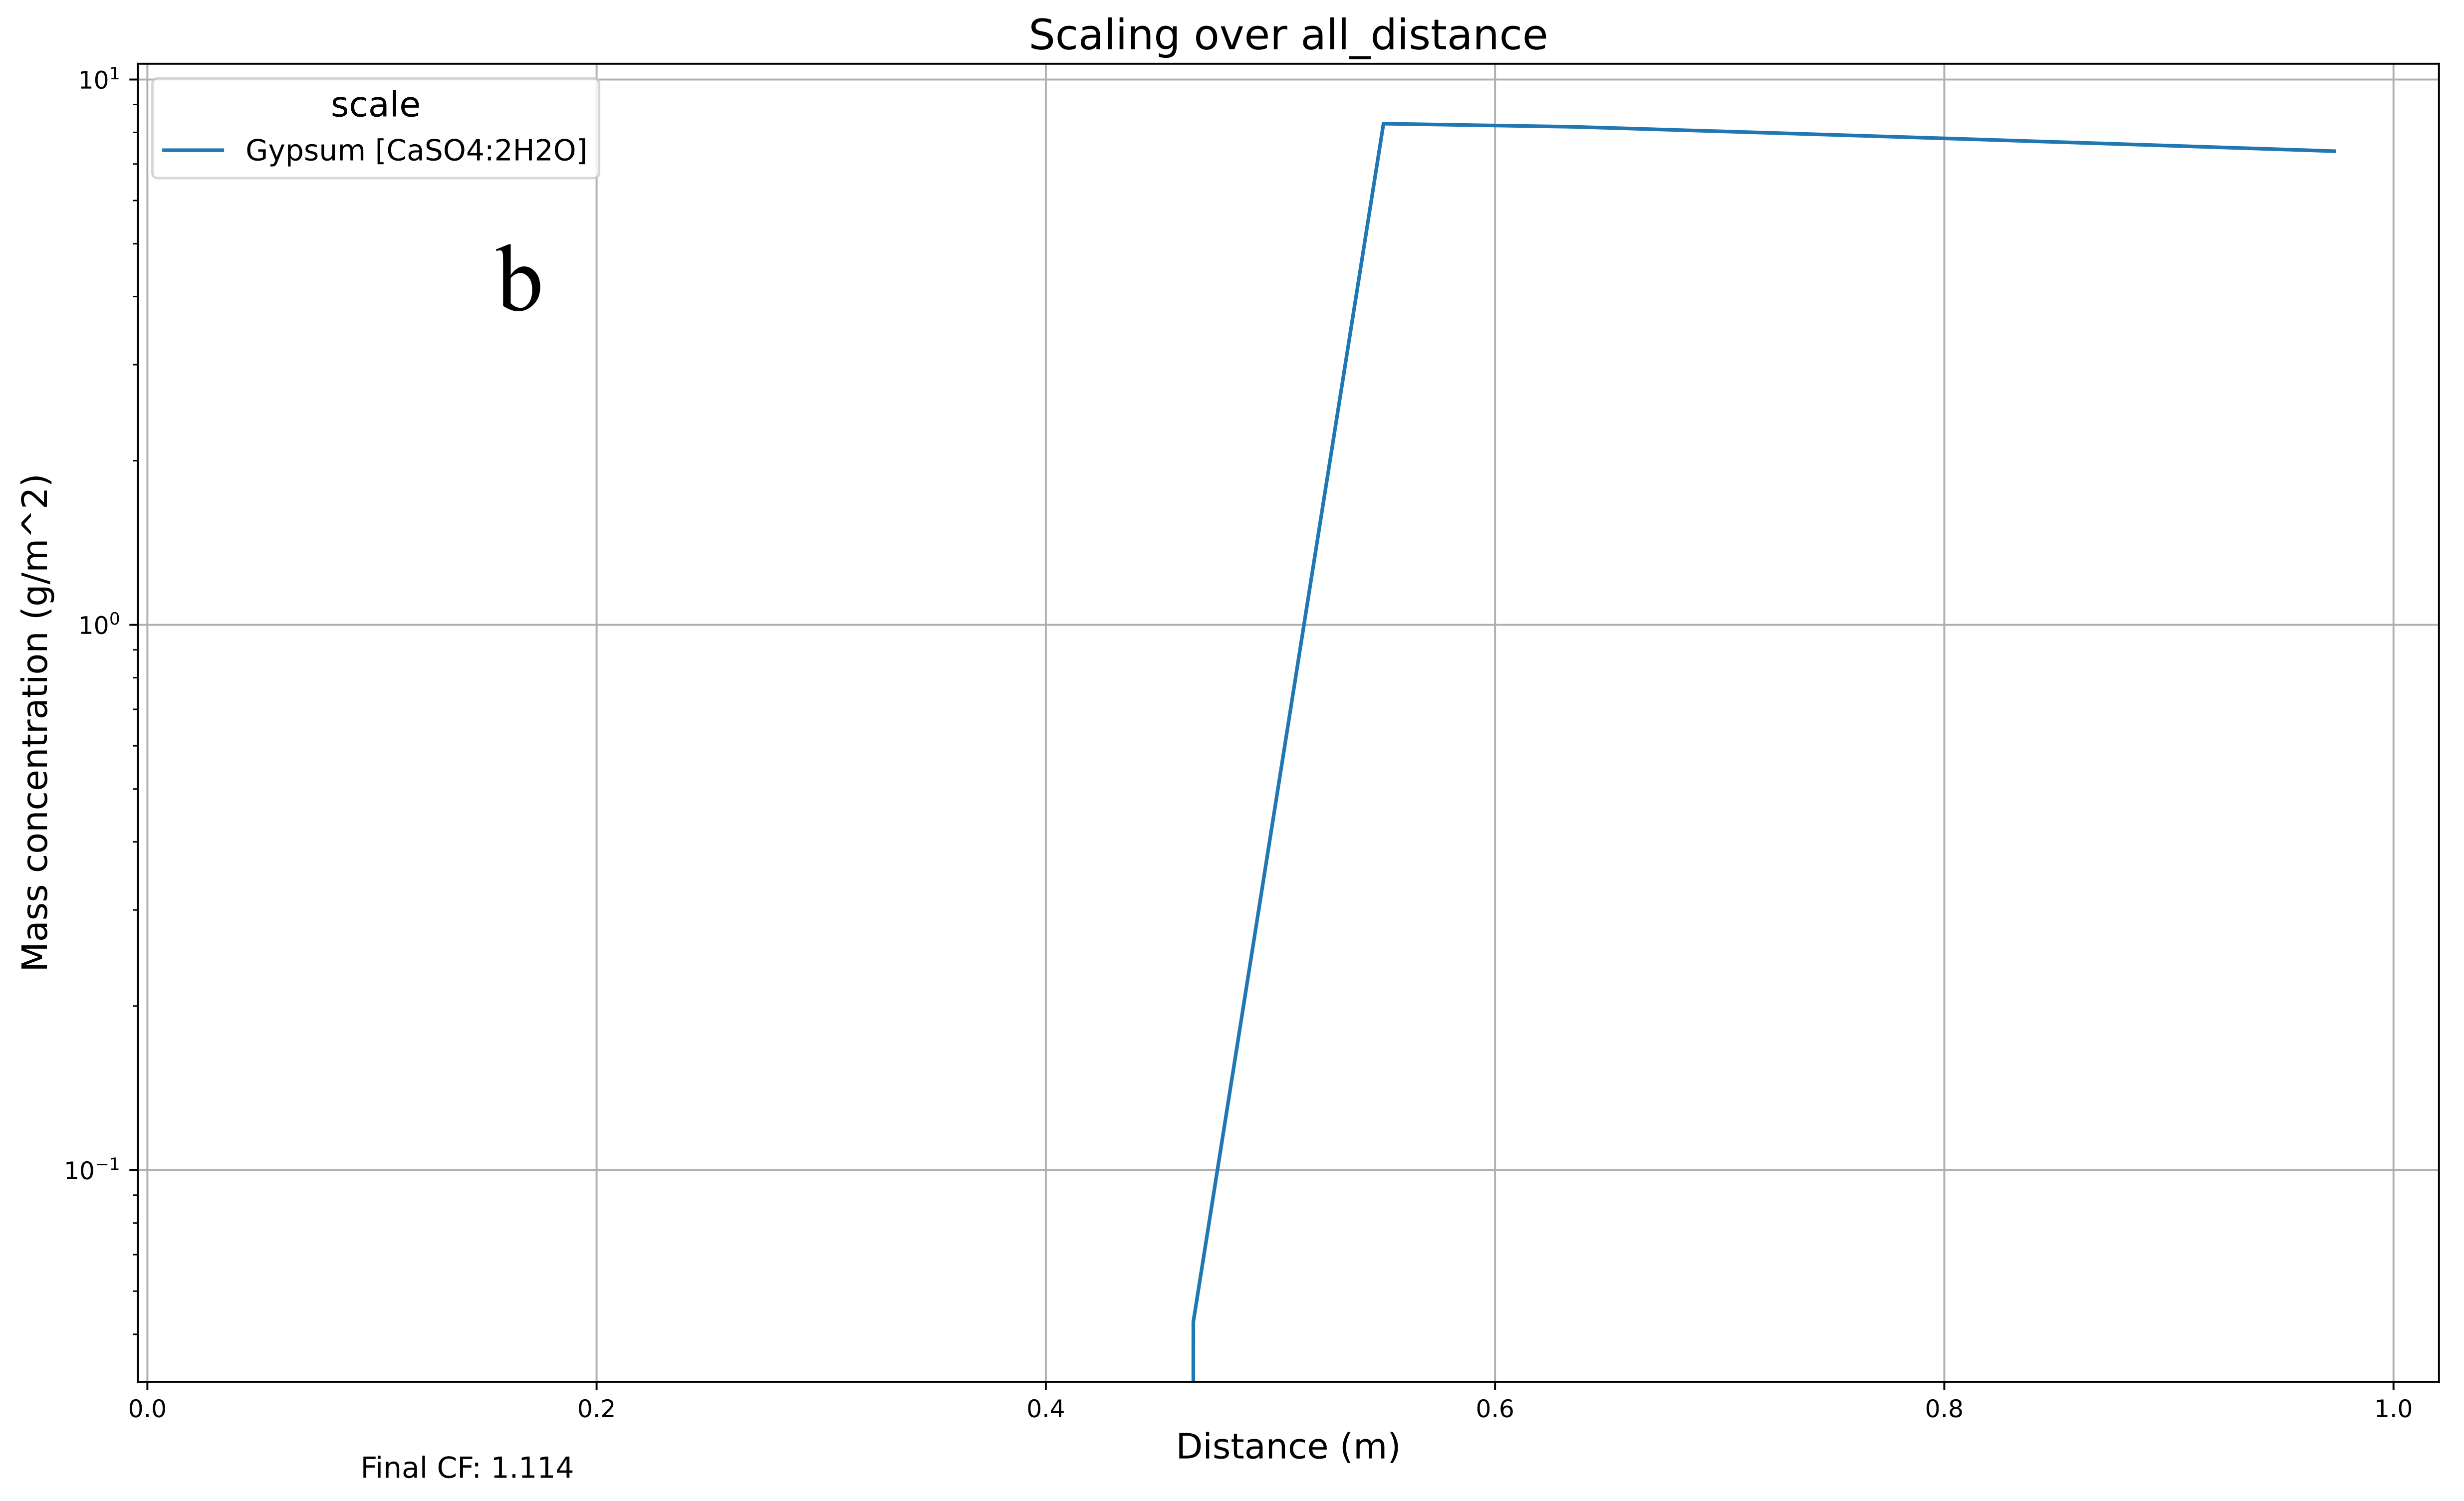
\includegraphics[width=\linewidth]{images/ROSSpy/sensitivity_analyses/simulation_perspective/all_distance.png} 
    \end{tabular}
    \caption{
        Scaling while either slicing through a) time at the final cell or b) distance at the final time. The underlying simulation was of the Red Sea through the BW30-400 module.
    }
    \label{scaling_perspectives}
\end{figure}

A cross-section of an RO module, which highlights boundaries of the single- and dual-domain solution models, is depicted in Figures \ref{single_dual_domain}.

\subsection{Software}

\subsection{PHREEQC consistency}

\subsubsection{ICE table calculations}
The expected precipitation in the presented ICE table of Table \ref{ice_table} was determined as $x$ in the following derivation:

\begin{equation} \label{ice_calculations}
    \begin{split}
        K_{sp} &= [a_{Ca^{2+}} - x]^1 * [a_{SO_4^{2-}} - x]^1 \\ 
        K_{sp} &= (\gamma*[Ca^{2+}] - x) * (\gamma*[SO_4^{2-}] - x) \\ 
        10^{-4.58} &= ((0.19*0.020594) - x) * ((0.06*0.105462) - x) \\ 
        10^{-4.58} &= (0.003913 - x) * (0.00633 - x) \\
        10^{-4.58} &= 2.477E-5 - 0.01024 + X^2 \\
        0 &= -1.54E-6 - 0.01022x + x^2 \\
         \therefore ~~ x &= 0.0104~molal = \frac{\fbox{0.181~moles}}{17.67~kg~water}~~.
    \end{split}
\end{equation}

The activity coefficients ($\gamma$) for $Ca^{2+}$ and $SO_4^{2-}$ were sourced from PHREEQC for this specific solution system. The $17.67~kg$ mass of water corresponds to the mass maximum capacity of the simulated BW30-400 module.  

The predicted precipitation in the presented ICE table of Table 1b ($gypsum\_pore\_volume$) are similarly derived:
\begin{equation} \label{PHREEQC_output_precipitation}
    \begin{split}
        gypsum\_pore\_volume &= gypsum\_all\_shifts * \frac{cells\_per\_module}{total\_simulation\_shifts} \\
         &= \sum_{i=1}^n (Gypsum_i) * \frac{12}{51} \\ 
         &= 0.823 * \frac{12}{51} \\ 
         &= 0.194 ~moles ~~.
    \end{split}
\end{equation}
The $\frac{12}{51}$ is the fraction of simulation shifts that correspond to a single module or pore volume, where the simulated module was discritized into $12$ cells. This isolates scaling from a single module, instead of the accumulation of scaling from multiple pore volumes, which renders the quantity directly comparable with the expected quantity.

\begin{table}[h]
    \centering
    \begin{tabular}{c|ccccc}
      \toprule
       & $Ca^{2+}$ & $+$ & $SO_4^{2-}$ & $\leftrightharpoons$ & $CaSO_4$ \\
      \midrule
      I & $0.003913$ && $0.00633$ && $0$ \\
      C & $-x$ && $-x$ && $+x$ \\
      F & $0.003913-x$ && $0.00633-x$ && $x$ \\
      \bottomrule
    \end{tabular}
    \caption{
        Gypsum precipitation according to the ICE (Initial, Change, Equilibrium) framework, except that "Equilibrium" (E) is replaced with "Final" (F) since the system does not reach equilibrium while within the module. The estimated Gypsum precipitation from a solution of $Ca^{2+}$ \& $SO_4^{2-}$ -- based upon the $K_{sp}$ of Gypsum and the activity coefficients of this solution from iPHREEQC -- is derived in \ref{ice_calculations} for the system in this table. 
        }
    \label{ice_table}
\end{table}

\subsubsection{Evaporation versus transport desalination}

The mechanism of concentrating a solution, either via evaporation or desalination, should not alter scaling predictions, ceterius paribus. Figure \ref{evaporation} contrasts scaling predictions from evaporation and desalination of the Red Sea, where the two mechanisms are approximately equivalent. Differences are postulated to originate from the consideration of advection in the latter but not the former.

\begin{figure}
    \centering
    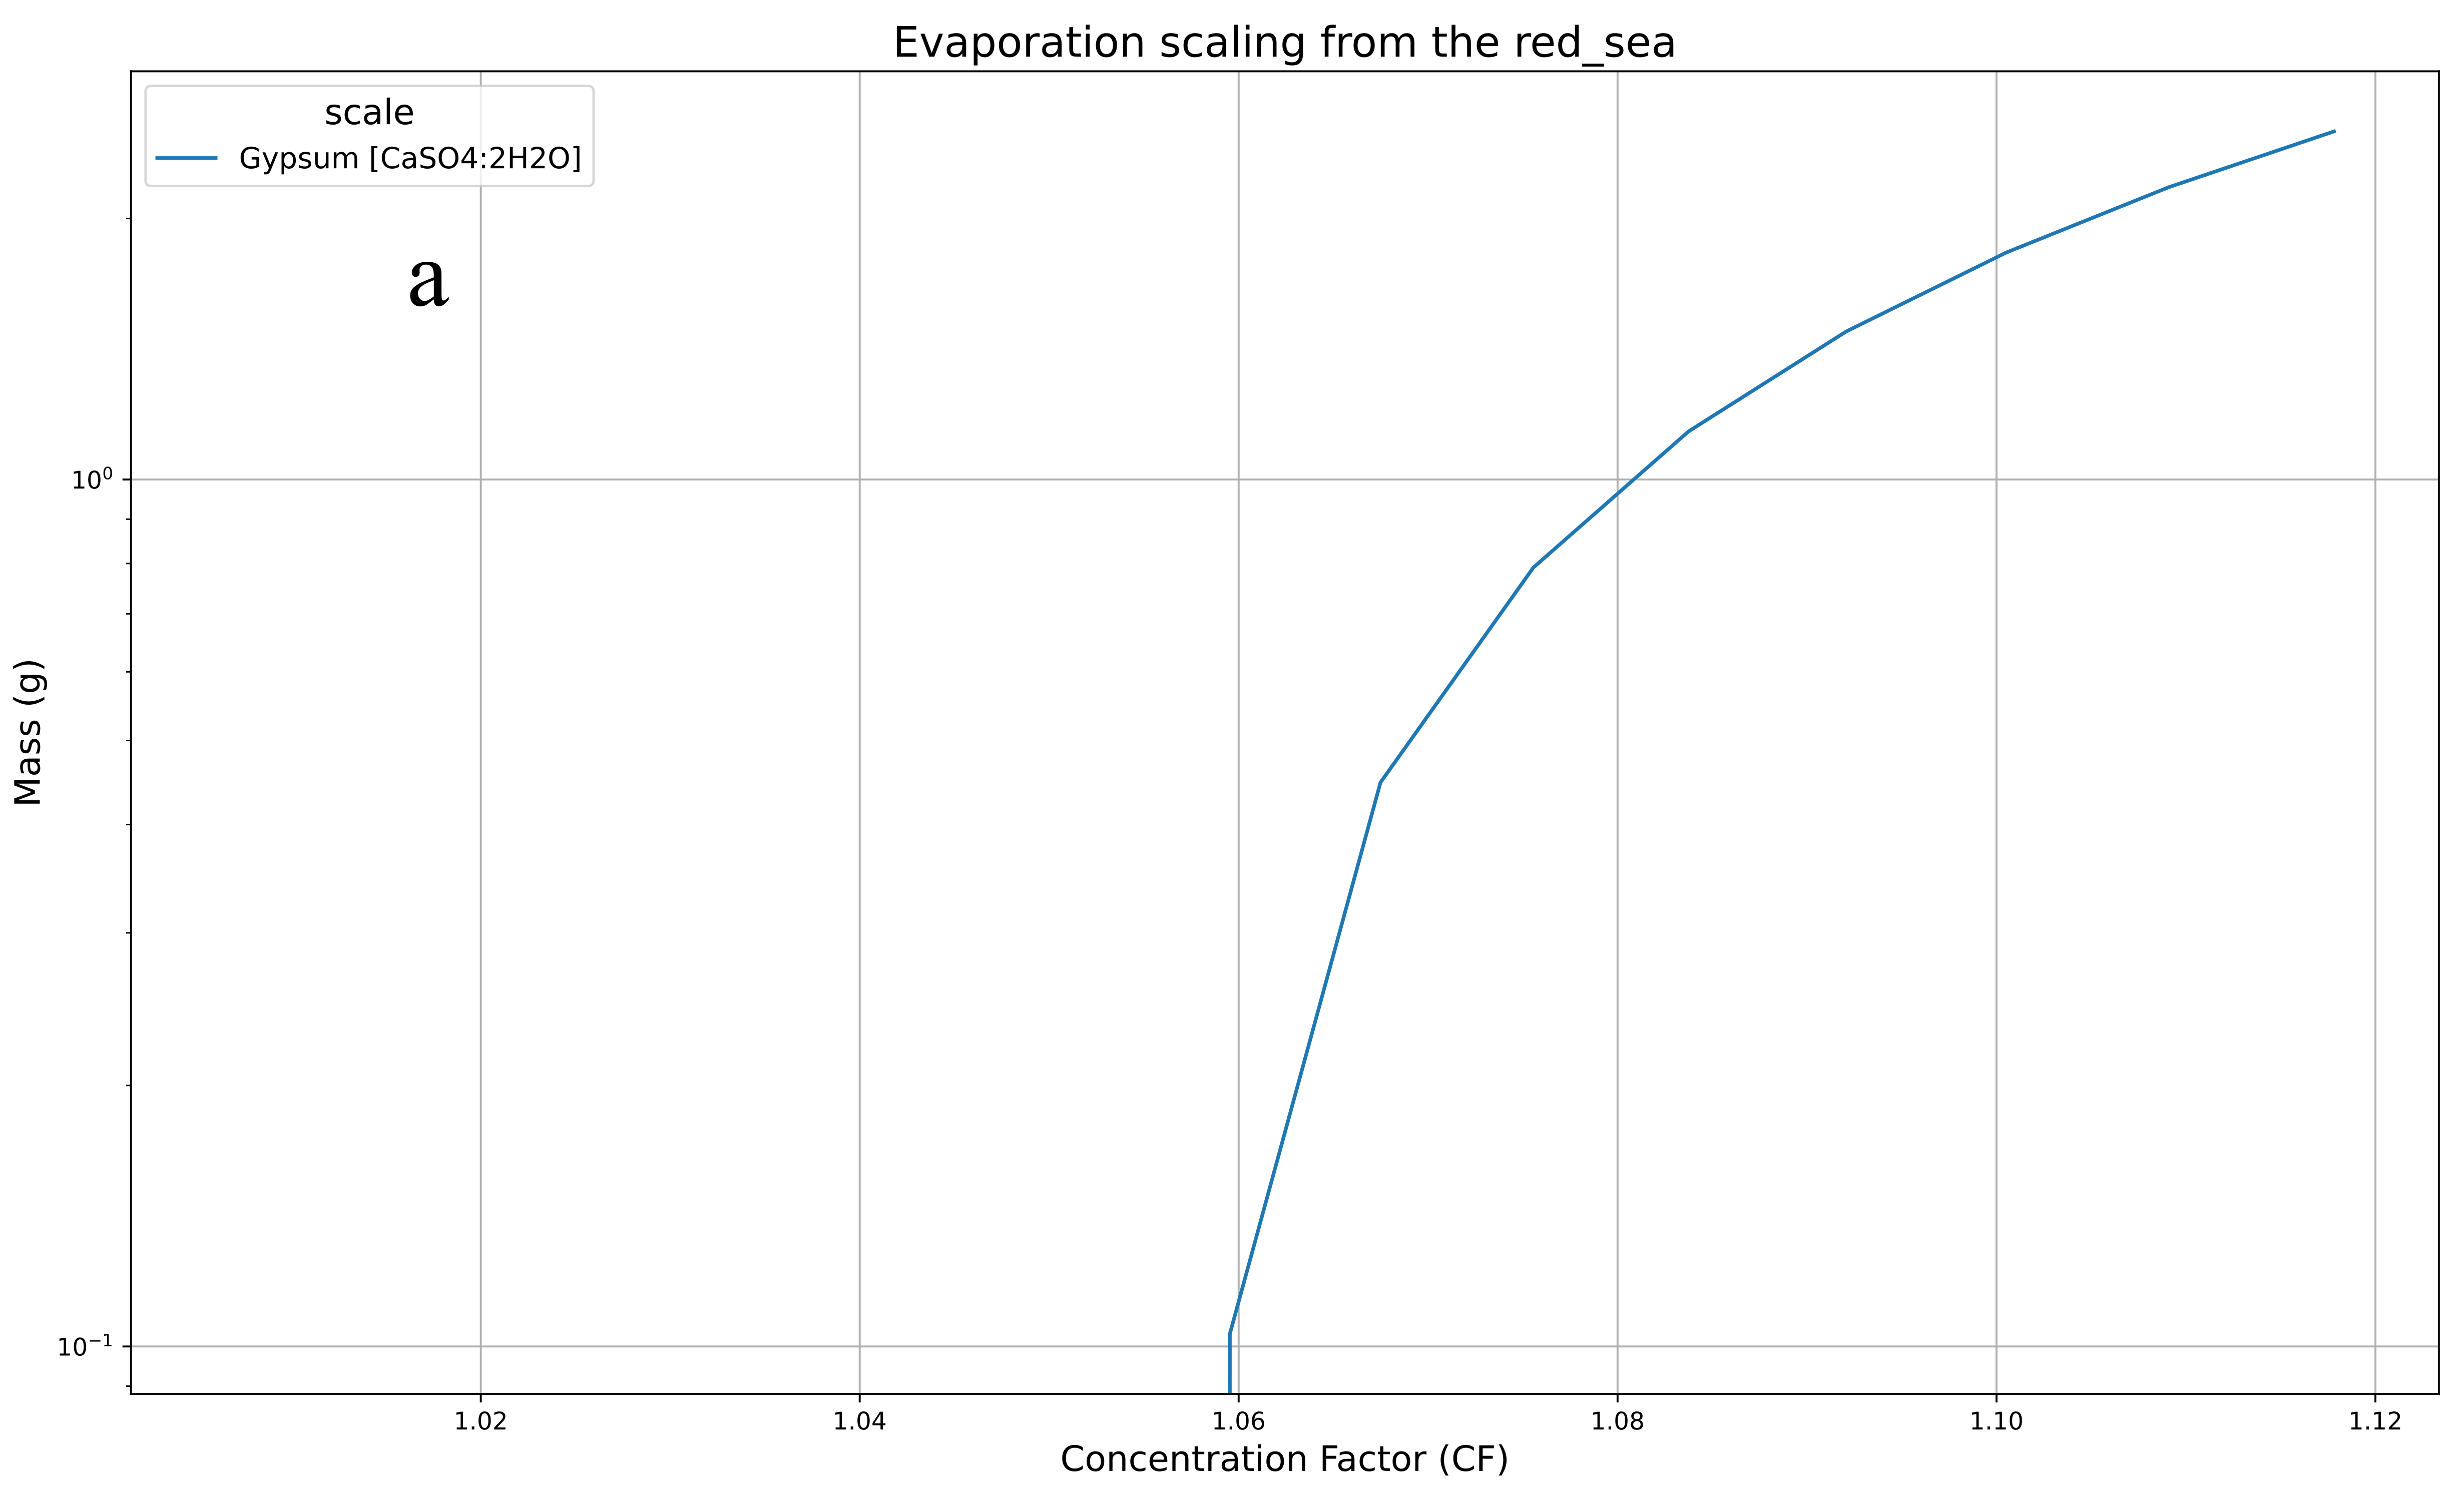
\includegraphics[width=\linewidth]{images/ROSSpy/sensitivity_analyses/evaporation/evaporation.png} \\ \midrule
    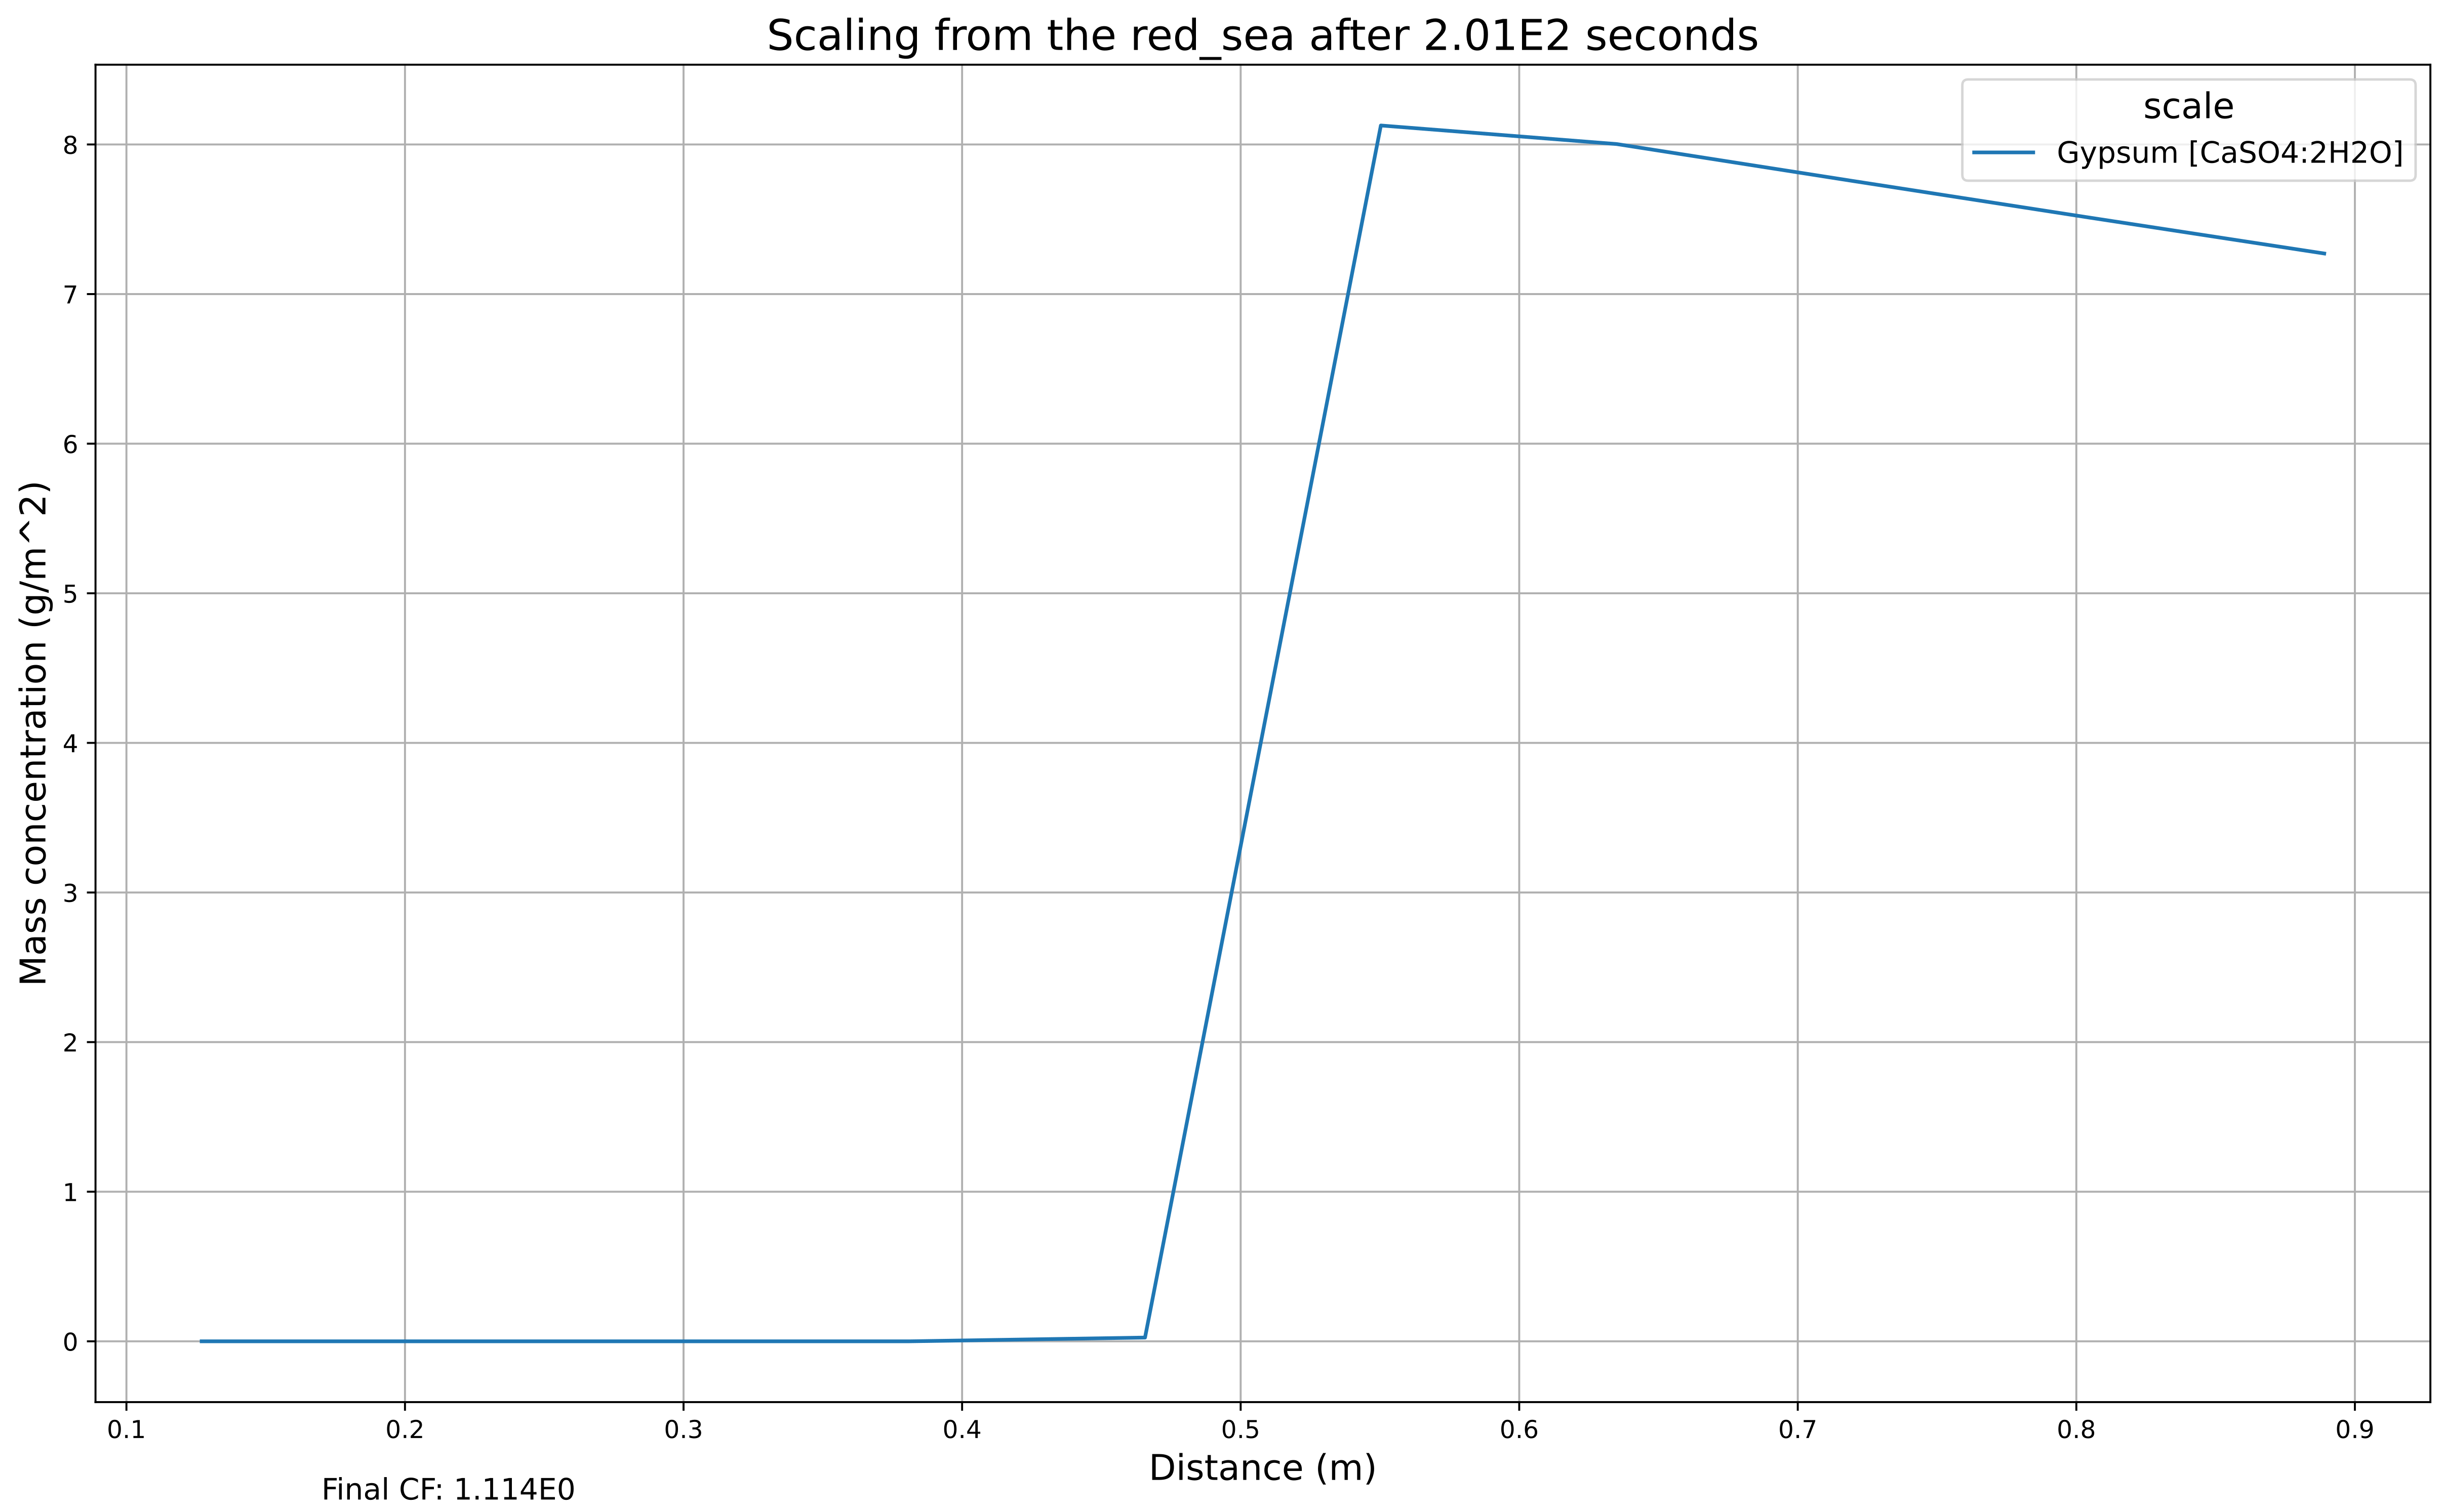
\includegraphics[width=\linewidth]{images/ROSSpy/sensitivity_analyses/evaporation/desalination.png}
    \caption{
        Scaling while a) evaporating and b) desalinating the Red Sea. The two scaling predictions are qualitatively similar, however, even after accounting for the accumulation amongst different pore volumes, the evaporation predictions ($3.36g$) are less than those of the reaction transport simulation ($5.27g$). The difference may be the absence of advection in the evaporation analysis.
    }
    \label{evaporation}
\end{figure}


\subsection{In-series RO arrangements}

In-series arrangements of multiple RO modules are represented by compounding individual modules. We determined that this approach is preferential to a few other methods: e.g. amplifying the characteristics of a single RO module, such as those in Table \ref{RO_dimensions}, by a scalar $r=\frac{\Phi_{\Delta multi-module}}{\Phi_{\Delta module}}$, where the $\Delta \Phi_{multi-module}$ is the total permeate flux of the multi-module system that can be parameterized or approximated through eq. (8). The substitution of $CF_{multi}$ for $CF_e$ and $\Delta \Phi_{multi-module}$ for $\Phi_e$ into eq. (9) permits calculating the $\Delta \Phi_{multi-module}$. 

\begin{savenotes}
\begin{table}[!h]
    \centering
    \begin{tabular}{|c|c|c|}
        \toprule
        \textbf{Parameter} & \textbf{Value} & \textbf{Source} \\ \midrule
        
        \multicolumn{3}{c}{Module (m)} \\ \midrule
        length & 1.016 & BW30-400 \cite{2020FilmTecElement} \\ 
        diameter & 0.201 & BW30-400 \cite{2020FilmTecElement}\\
        permeate tube diameter & 0.029 & BW30-400 \cite{2020FilmTecElement}\\ \midrule
        
        \multicolumn{3}{c}{Membrane (mm)} \\ \midrule
        filtration layer & 0.00025 & \cite{Pacheco2010CharacterizationTechniques,Jeong2007InterfacialMembranes} \\
        Feed spacer & 0.8636 & BW30-400 \cite{2020FilmTecElement} \& \cite{Sablani2002InfluenceSystems} \\
        Permeate spacer & 0.3 & \\
        Polysulphonic layer & 0.05 &  \\
        Support layer & 0.15 &  \\
        Windings $\left( \frac{th_{total}}{th_{membrane}} \right) $ & 86 & BW30-400 \cite{2020FilmTecElement} \\ \midrule
        
        \multicolumn{3}{c}{Membrane cross-section ($m^2$)} \\ \midrule
        Module & 0.0317 & BW30-400 \cite{2020FilmTecElement}\\
        Permeate tube & 0.000661 & BW30-400 \cite{2020FilmTecElement}\\
        Filtration section & 0.0311 & BW30-400 \cite{2020FilmTecElement}\\
        Feed channel & 0.0157 & BW30-400 \cite{2020FilmTecElement}\\ \midrule
        
        \multicolumn{3}{c}{Feed channel capacity} \\ \midrule
        Volume ($m^3$) & 0.0159 & BW30-400 \cite{2020FilmTecElement}\\
        Mass (kg) & 15.86 & BW30-400 \cite{2020FilmTecElement}\\ \midrule

        \multicolumn{3}{c}{Fluid flow ($\frac{m^3}{second}$)} \\ \midrule
        Permeate & 0.000463 & BW30-400 \cite{2020FilmTecElement}\\
        Max Feed & 0.00442 & BW30-400 \cite{2020FilmTecElement}\\ \bottomrule
        
    \end{tabular}
    \caption{
        Default dimensions of an RO module, with corresponding citations, that are primarily based upon the DOW FILMTEC BW30-400 RO module, following precedence from other software \cite{Li2012OptimalDesalination}.
    }
    \label{RO_dimensions}
\end{table}
\end{savenotes}

\subsection{Water bodies}

Additional feed parameter files can be composed by emulating the structure of the default feed parameter files. Literature sources that may foster the development of such feed parameter files for numerous potential feed sources are provided in Table \ref{new_water_bodies} with the respective citations of the experimental geochemical data. 

\begin{table}[h!]
    \centering
    \begin{tabular}{|c|c|}
        \toprule
        \textbf{Water body} & \textbf{Geochemical measurements} \\
        \midrule
        Indian Ocean & \cite{Danielsson1980CadmiumWater,Nisha2014GeochemicalIndia,Stephen-Pichaimani2008EnrichmentIndia,Selvaraj2004EvaluationApproaches,Thangadurai2005Pre-tsunamiIndia,ParvezAl-Usmani2015TraceIndia,Sabine2002InorganicProcesses,Singh2013InternalBengal} \\
        Sargasso Sea & \cite{Bender1976DissolvedSea,Stoffyn-Egli1984MassOceans} \\
        South China Sea & \cite{Calvert1993GeochemistrySeas,Wen2006PhysicochemicalSea,Du2020DynamicsStudy,Chen2001NutrientBasin,Nakaguchi2004DissolvedSea} \\
        Greek Coast & \cite{Chester1981TheSediments,Voutsinou-Taliadouri1983DistributionGreece,Voutsinou-Taliadouri1997DissolvedSeawater} \\
        Toyko Bay & \cite{Fukushima1992TraceJapan} \\
        California Coast & \cite{Hershelman1981MetalsOutfall,Luoma1988DistributionBay,Biller2013SourcesSeason} \\
        North Atlantic & \cite{Loring1978GeochemistryLawrence.,Loring1979GeochemistryLawrence,Yeats1983PotentialAtlantic,Bothner1998MetalTime,Campbell1980BaselineBay,Gaulier2019TraceWaters,Statham1986Dissolved0-35N,Mohamed2011DissolvedOcean,Guay1998ASeas} \\
        Baltic Sea & \cite{Szefer1995DistributionSea,Kremling1978TheStation} \\
        North Pacific & \cite{Tanita2015SurfacePacific,Sim2019Annual20102013} \\
        South Pacific & \cite{Boyle1975CopperZealand,Boyle1976OnCadmium} \\
        General natural waters & \cite{Alibo1999RareOxidation,Klinkhammer1983RareVents,Garcia-Solsona2020RareSea,Longinelli1967Oxygen-18Lakes,Llyod1967Oxygen-18Sulfate,Culkin1966SodiumWater,Krumgalz1982CalciumWaters} \\
        Mississippi Salt Dome Basin & \cite{Kharaka1987GeochemistryU.S.A.} \\
        \bottomrule
    \end{tabular}
    \caption{
        Proposed literature of potential feed water that can be adapted into parameter files for simulation in our model, or specifically ROSSpy.
    }
    \label{new_water_bodies}
\end{table}

\subsection{Dual domain}

\begin{figure}
    \centering
    \begin{tabular}{c|c}
        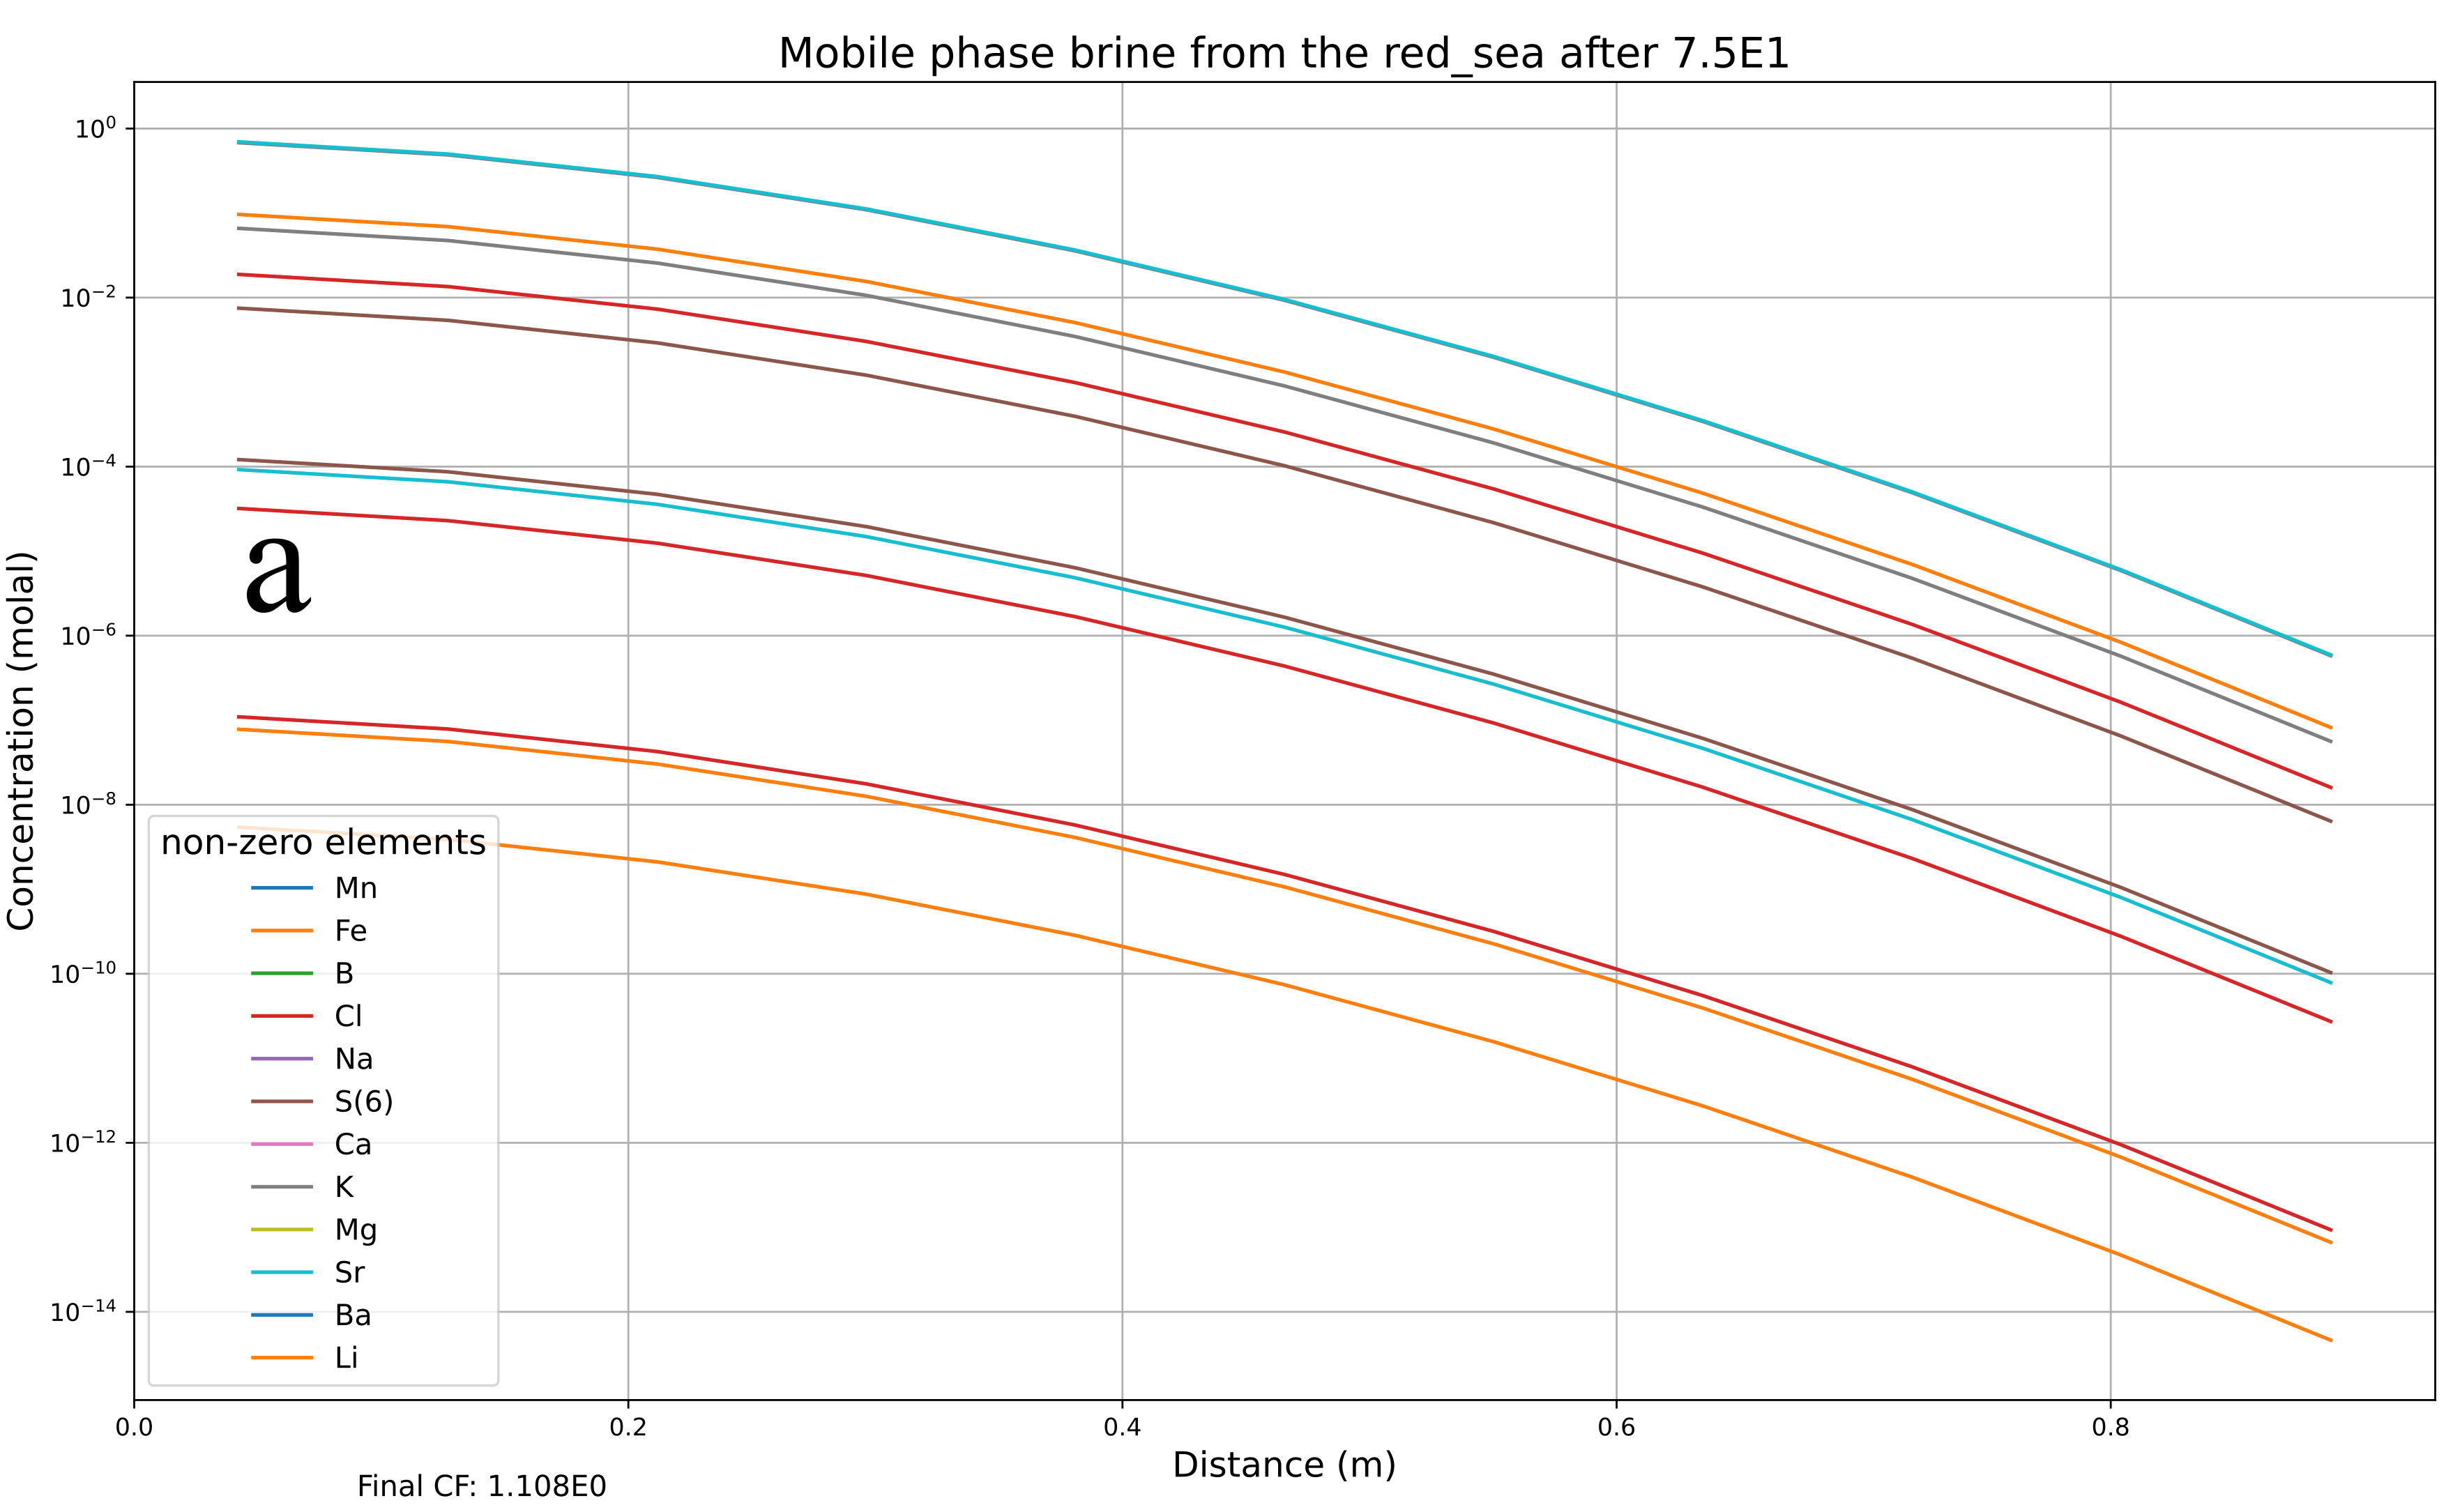
\includegraphics[width=0.49\textwidth]{images/ROSSpy/sensitivity_analyses/EF/mobile_large_ef.png} &
        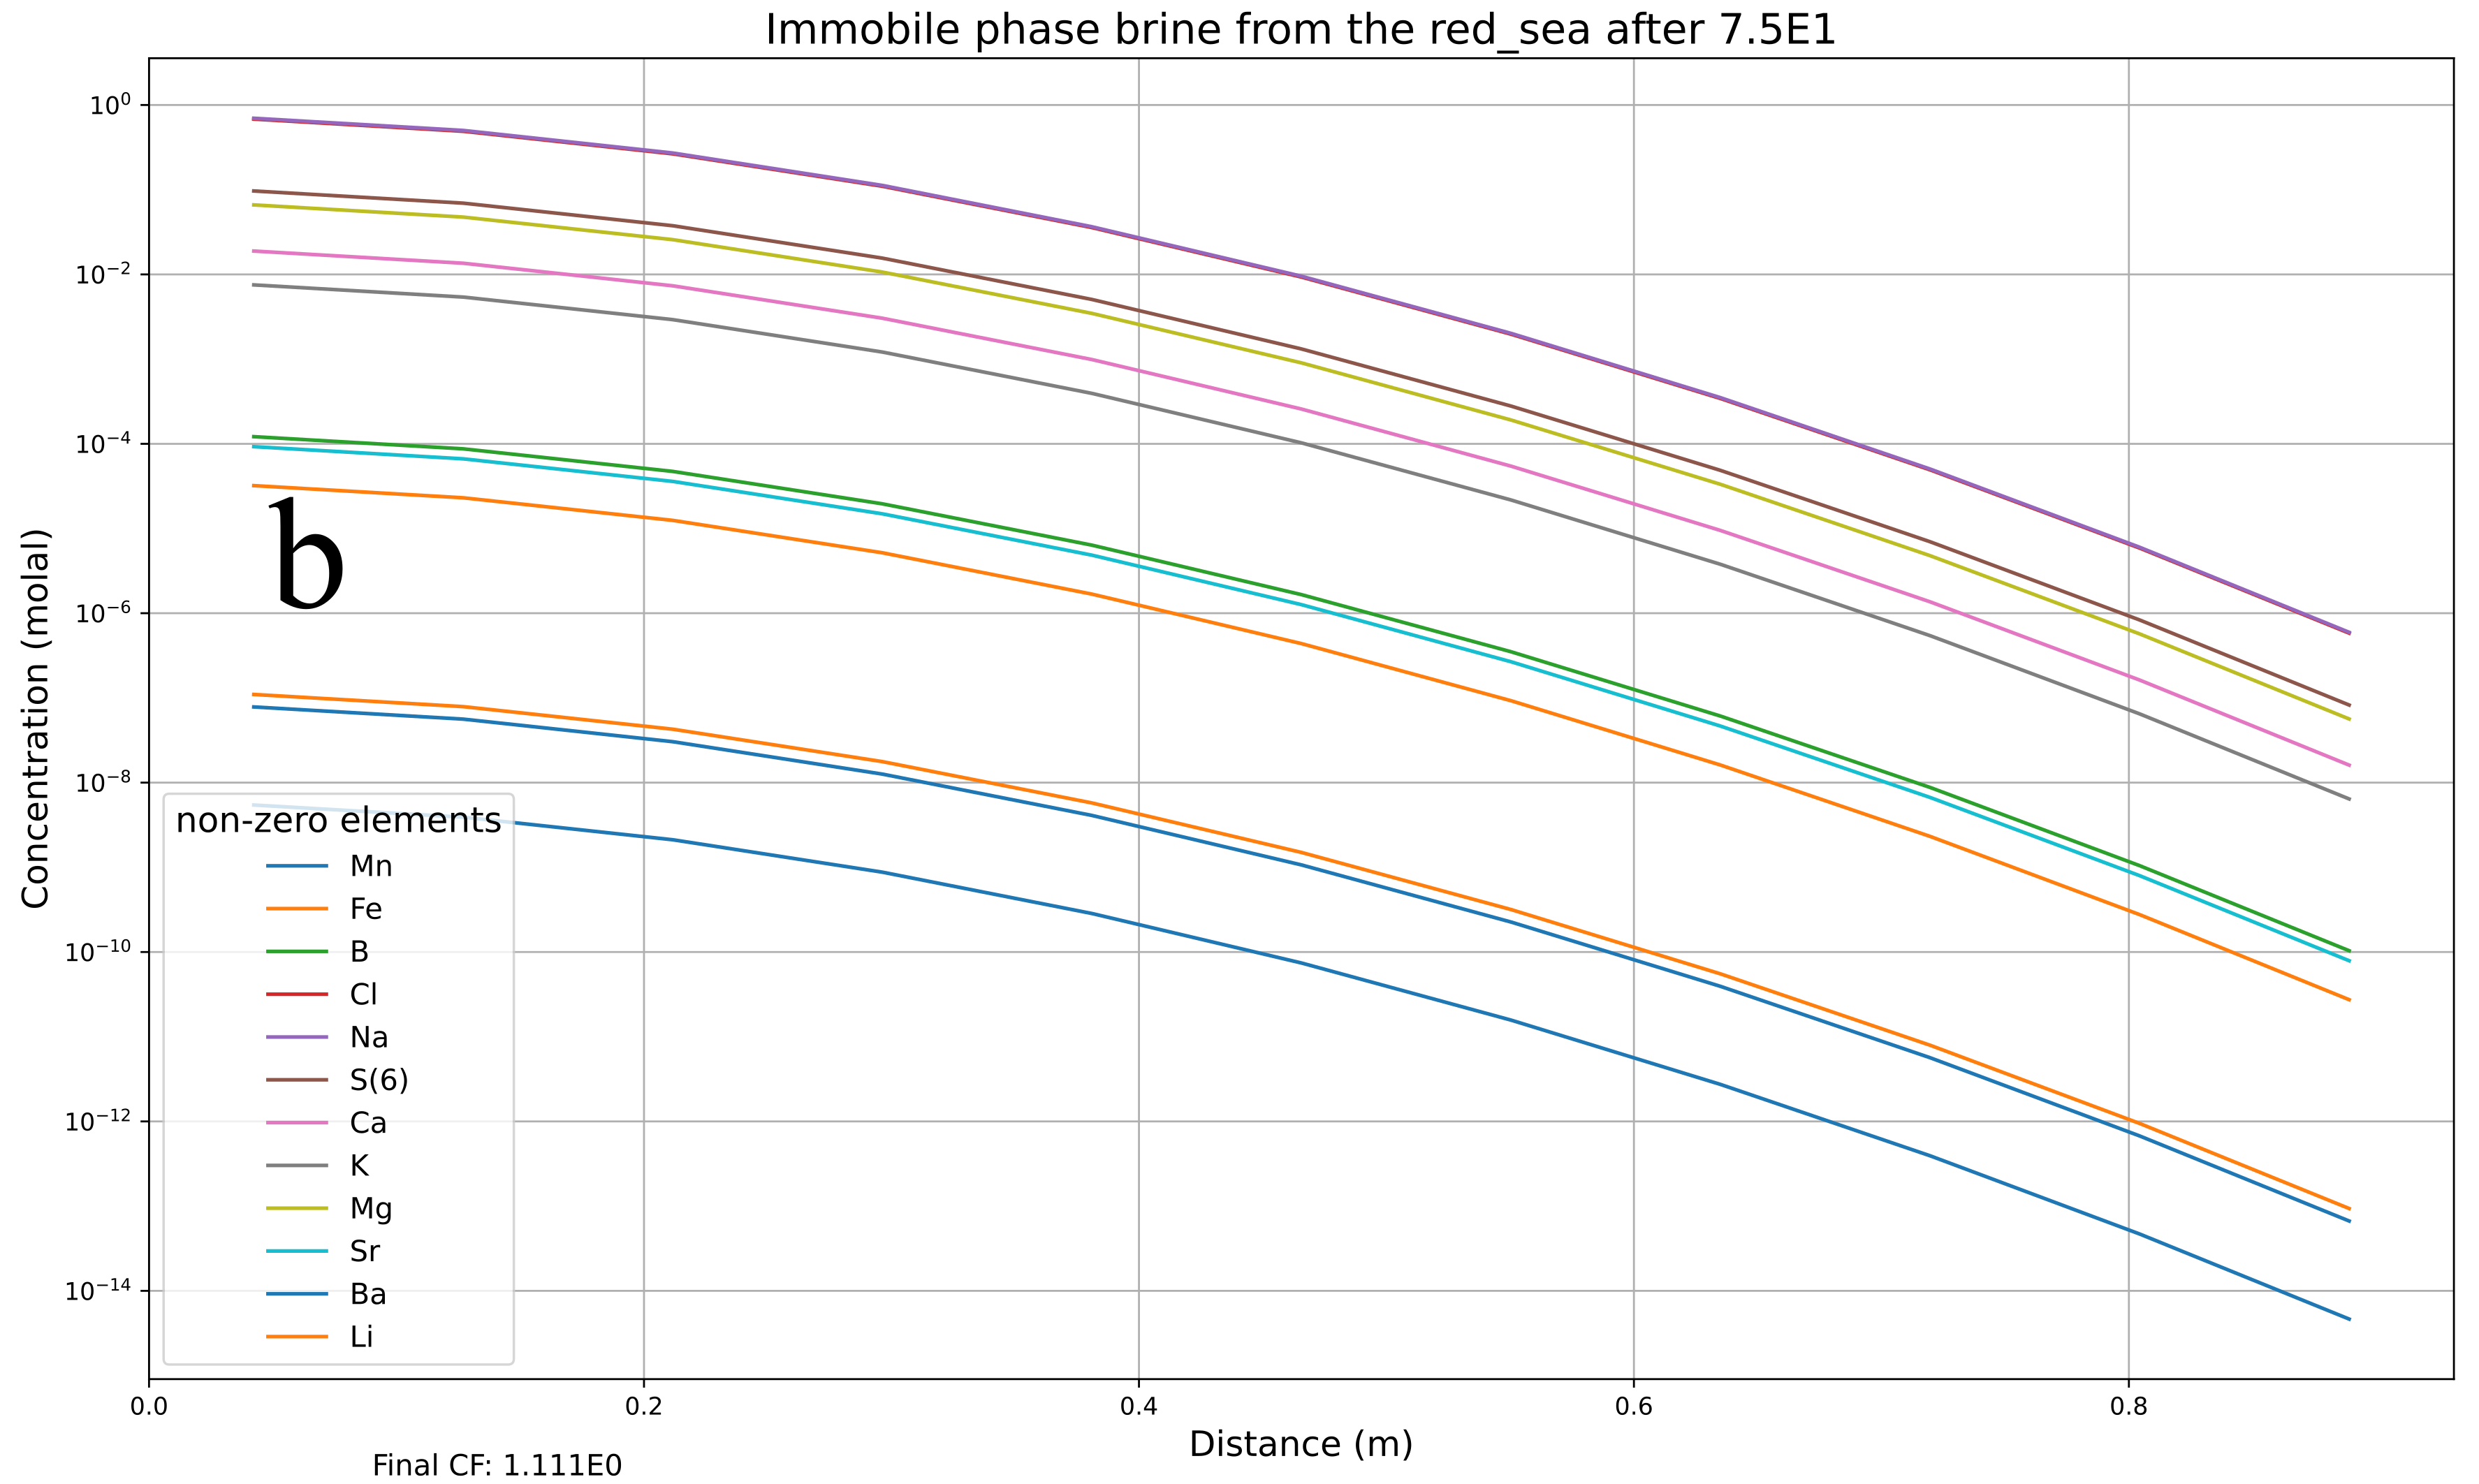
\includegraphics[width=0.49\textwidth]{images/ROSSpy/sensitivity_analyses/EF/immobile_large_ef.png} \\ \midrule
        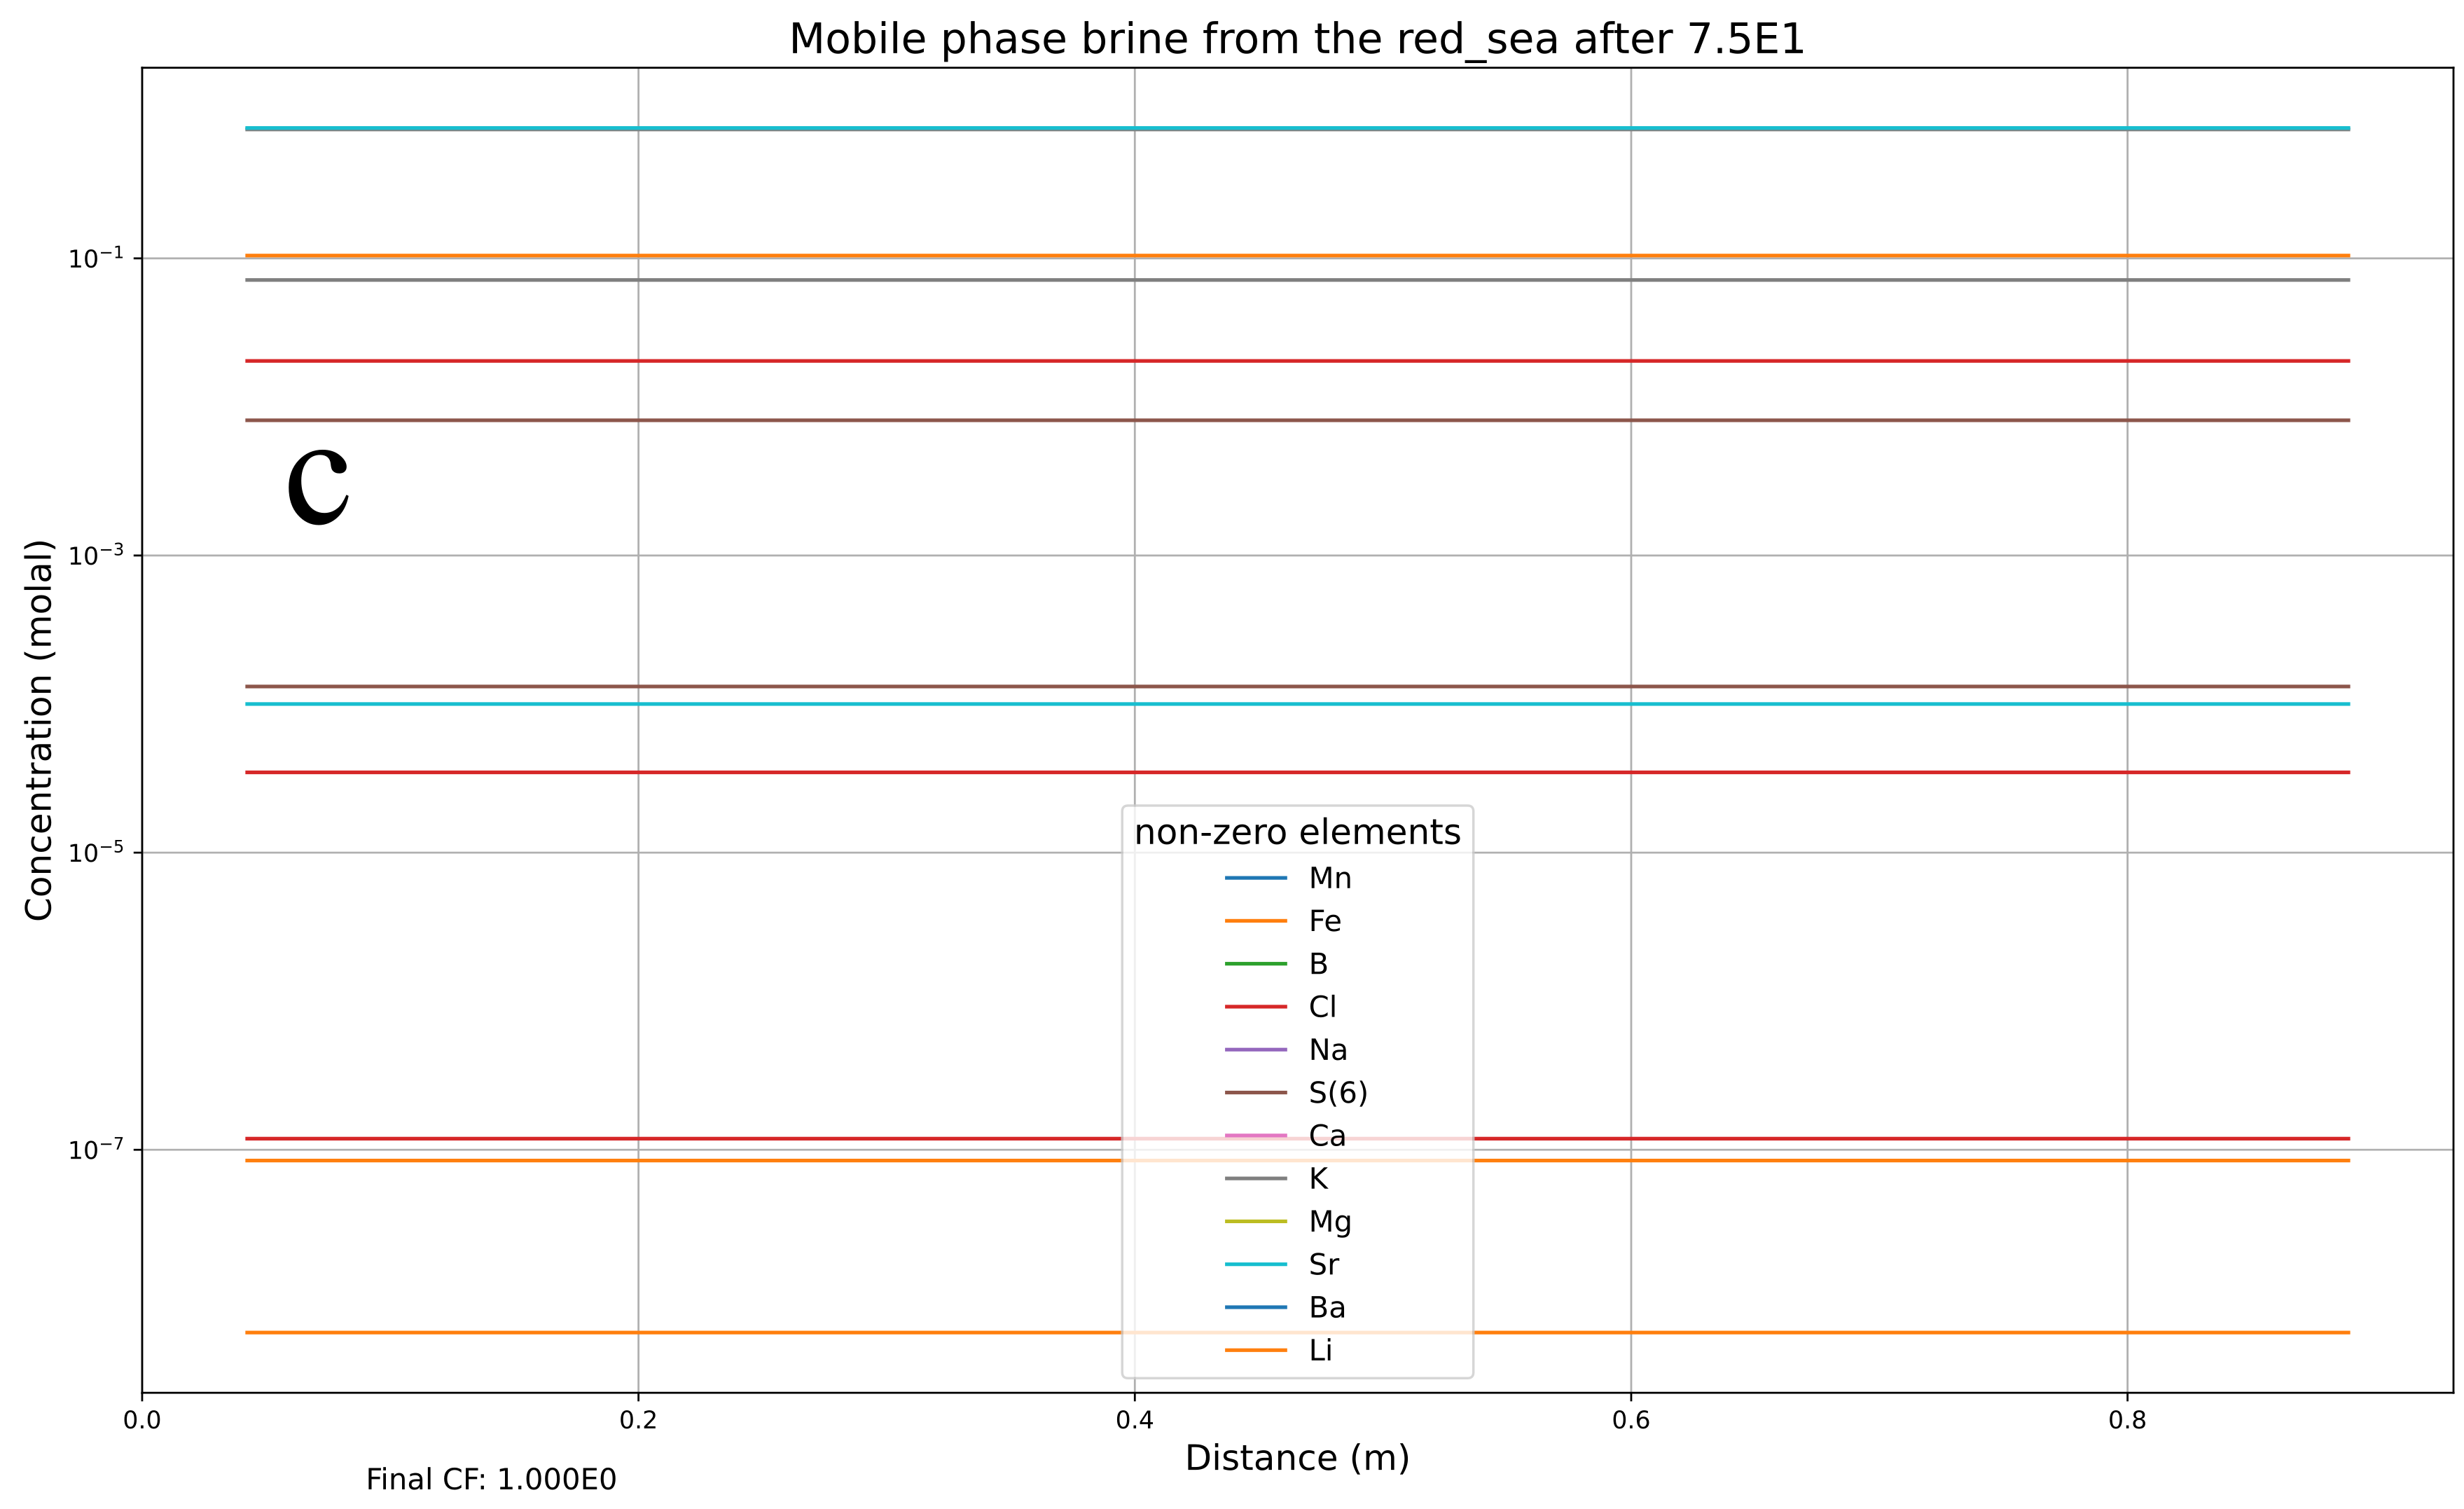
\includegraphics[width=0.49\textwidth]{images/ROSSpy/sensitivity_analyses/EF/mobile_small_ef.png} & 
        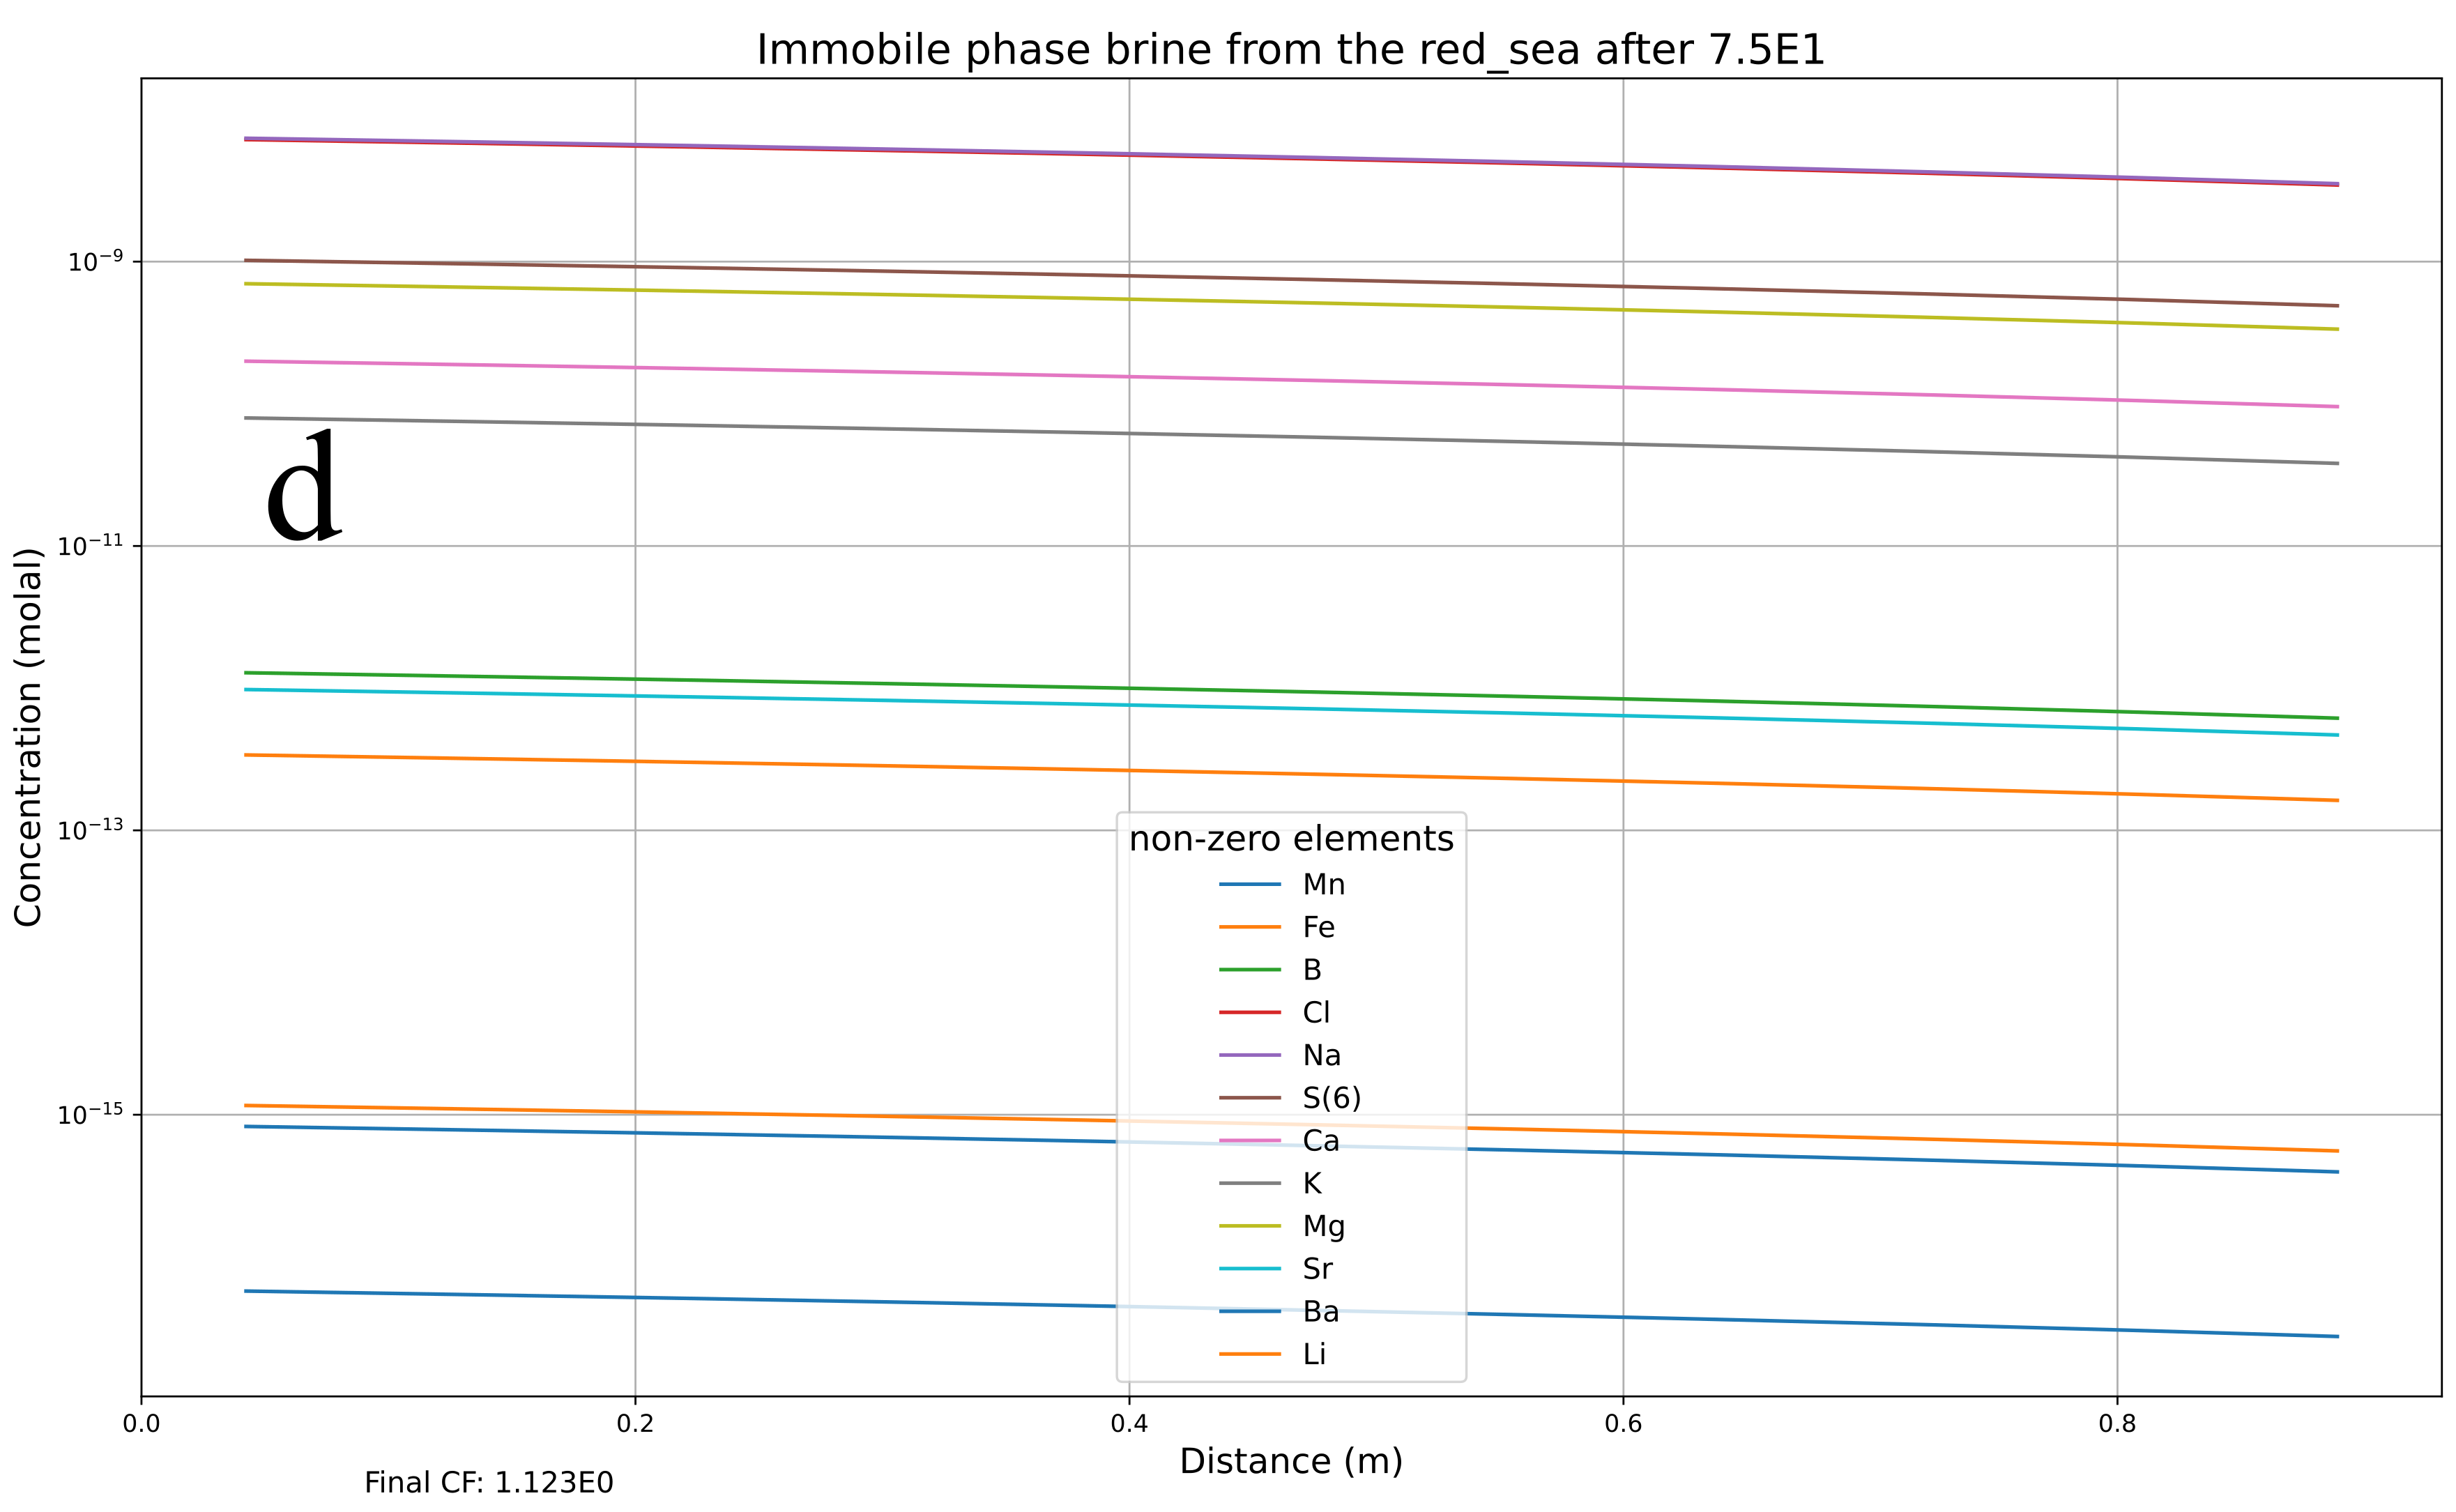
\includegraphics[width=0.49\textwidth]{images/ROSSpy/sensitivity_analyses/EF/immobile_small_ef.png} \\ \bottomrule
    \end{tabular}
    \caption{
        Counter-intuitive brine predictions from dual domain simulations with different exchange factor (EF) values, which is the $\frac{1}{s}$ rate constant of solvent exchange between the mobile and immobile solution phases. Panels a) and b) depict the mobile (bulk) and immobile (CP) phases when $EF=1E10$, while panels c) and d) depict the mobile and immobile phases when $EF=1E-10$, respectively. These non-sensible results motivated our use of the single-domain model to represent RO feed flow. 
    }
    \label{ef_values}
\end{figure}

Our model represents the feed solution with the single-domain model, despite that the dual-domain model in the module cross-section of Figure \ref{single_dual_domain} is more fundamentally accurate, since our attempts to encode the latter in PHREEQC have been unsuccessful. We represent the mobile phase (bulk solution) as one set of membrane cells -- $[1,n]~n\in W$ -- and the immobile phase (CP layer) as a separate set of cells -- $[n+2,m]~m \in W>n+2$. These cell sets exchange solvent at a parameterized rate -- the Exchange Factor $\frac{1}{s}$ (EF) -- which in Figure \ref{ef_values} is very influential upon the simulation predictions; however, the brine concentrations dilute in both solution compartments during desalination simulation. The scaling predictions are equally non-sensible. Our model therefore uses the single-domain model, which appears to be an acceptable approximation per our validations. The developer of PHREEQC -- David Parkhurst -- is uncertain whether the dual-domain model is compatible with the PHREEQ code, which assures us that the single domain model may be the best approximation of desalination reactive transport that is accessible to our open-source framework.

\begin{figure*}
    \centering
    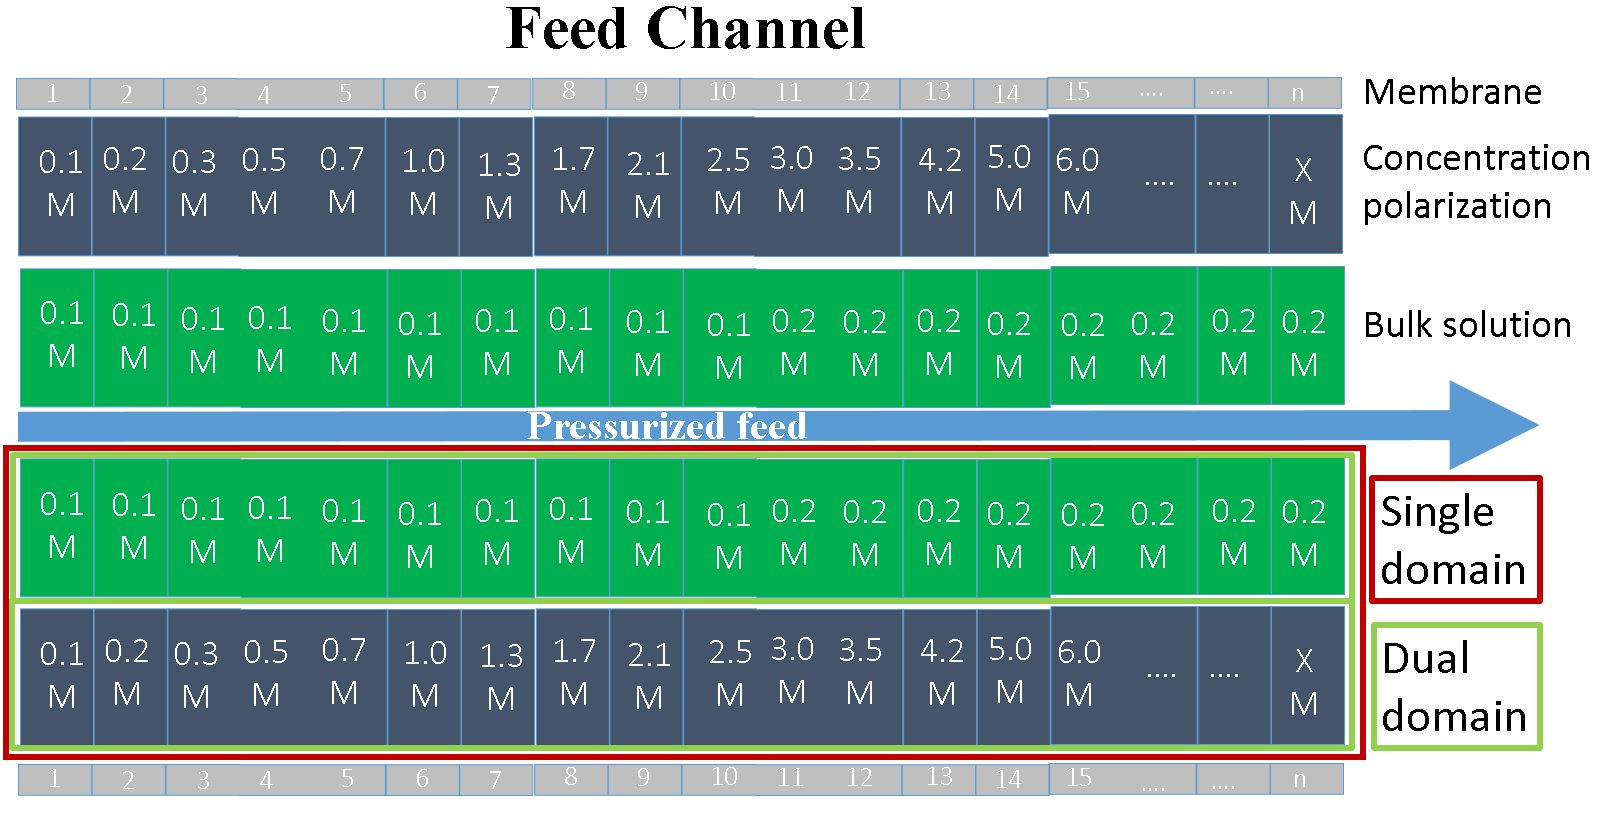
\includegraphics[width = \textwidth]{images/ROSSpy/supporting_information/single_dual_domain.jpg}
    \caption{
        A conceptual cross-section of the RO module. The membrane layers on top and bottom of the figure are discretized into an arbitrary $n$ cells. The figure illustrates the reactive transport phenomena, where the feed solution progressively becomes more concentrated as it transports through the module. The CP layer becomes much more concentrated than the bulk solution as a consequence of the no-slip boundary condition, where the velocity gradient reaches zero at the membrane surface and thus does not diffuse. These bulk and CP solutions are resolved in the dual-domain model (green boxed regions) and are granulated into a single solution by the single-domain model (red boxed regions). The latter was implemented in our model by necessity of PHREEQC.
    }
    \label{single_dual_domain}
\end{figure*}

\subsection{PHREEQ}
The most pertinent calculations of PHREEQC for our model are summarized in the following sub-section, while the version 3 PHREEQC User's manual provides a rigorous description of all PHREEQC operations.

\subsubsection{PHREEQ calculations}
\subsection{PHREEQ calculations}
The total concentration $\Psi_i$ of ionic species $i$ is calculated in each timestep, 
\begin{equation} \label{total_species_concentration}
    \Psi_i=C_i+\sum_{j=1}^{J}(v_{ij}*C_j),
\end{equation}
where $C_i$ is the molal concentration of dissolved $i$; $J$ is the set of compounds that contain $i$; $C_j$ is the molal concentration of compound $j$ that contains $i$; and $v_{ij}$ is the stoichiometric coefficient for the moles of $i$ per mole of compound $j$. The mineral precipitation equilibria over the simulation time $t$ is calculated through a similar equation, 
\begin{equation} \label{concentration_change}
    \frac{\partial \Psi_i}{\partial t}=\sum_{m=1}^{N_m}(v_{mj}*R_m),
\end{equation}
where $N_m$ is the set of reactions that include specie $i$; $v_{mj}$ is the stoichiometric coefficient for the moles of $i$ per mole of mineral $m$; and $R_m$ is the reaction flux of dissolution or precipitation for $(+)$ and $(-)$, respectively,
\begin{equation} \label{mineral_precipitation_reaction}
    R_m=sgn[\Omega]*A_m*k_m*(\Pi(a^n)) |e^{\frac{\eta*\Delta G}{RT}}-1|^p,
\end{equation}
where $\Omega = log\left(⁡\frac{Q_{dissolution}}{K_{sp}}\right)$ and, for the simulated mineral $m$, $A_m$ is the reacting surface area; $k_m$ is the rate constant of dissolution or precipitation; $Q_m$ is the ion activity product constant; and $\eta$ and $p$ are experimentally determined parameters. The $|e^{\frac{\eta * \Delta G}{RT}}-1|^p$ term simplifies to $1$ for irreversible precipitation or dissolution. The set of \cref{total_species_concentration,concentration_change} necessitates that any perturbations to ionic concentrations $\frac{\partial \Psi_i}{\partial t}$ manifest from complexation equilibria. The molal concentration $C_j$ of compound $j$ is discerned,
\begin{equation}
    C_j=\frac{\Pi_{j=1}^{N_c} (\gamma_j*K_j )^{v_{ij}}}{\gamma_j*K_j},
\end{equation}
where $N_c$ is the set of linearly independent chemical reactions; $\gamma_j$ is the activity coefficient of compound $j$; and $K_j$ is the equilibrium constant
\begin{equation}
    K_j=a_j \Pi_m^{M_{aq}} (a_m)^{-v_{m,j}},
\end{equation}
where $M_{aq}$ is the number of minerals in the aqueous system; $v_{m,i}$ is the stoichiometric coefficient of compound $j$ per mole of mineral $m$; and $a_j$ and $a_m$ are the activity coefficients of compound $j$ and mineral $m$, respectively. The activity coefficient $\gamma_j$ is calculated through either the Debye-Hückel model \cite{Aqion2016ActivityModels},
\begin{equation}
    log⁡(\gamma_j)=-A*z_j^2\sqrt{\mu},
\end{equation}
the WATEQ Debye-Hückel model \cite{Aqion2016ActivityModels},
\begin{equation}
    log⁡(\gamma_j)=\frac{-A*z_j^2*\sqrt{\mu}}{1+B*a_j^0*\sqrt{\mu}}+b_j \mu,
\end{equation}
the Davies model \cite{Davies1938TheSulphates},
\begin{equation}
    log⁡(\gamma_j)=-A*z_j^2 (\frac{\sqrt{\mu}}{1+\sqrt{\mu}}-0.2\mu),
\end{equation}
or the empirical Pitzer model \cite{Pitzer1973ThermodynamicsEquations}, where $A$ and $B$ are experimentally determined parameters; $a_j^0$ and $b_j$ are fitted parameters; $z_j$ is the charge of compound $j$; and $\mu$ is the ionic strength of the solution
\begin{equation}
    \mu=\frac{1}{2}\sum_{j=1}^{N_{aq}}z_j^2 \frac{n_j}{W_{aq}},
\end{equation}
where $W_{aq}$ is the simulated water mass and $n_j$ 
\begin{equation}
    n_j=C_j*W_{aq}=\frac{K_i*W_{aq}}{\gamma_j*(\Pi_m^{M_{aq}} (a_m)^{v_{m,j}}}
\end{equation}
is the moles of compound $j$. These calculations and geochemical models are more thoroughly described in the PHREEQC manual and in the cited literature.


\end{supplementary}

\newpage
\startchapter{A suite of packages for scalable Whole Cell Models: WCMpy}
\label{WCMpy_chapter}

\section{Introduction}
The development of whole-cell models (WCMs) \cite{Bhat2020Whole-CellSurvey} is purported to be a defining challenge of the 21st century \cite{Tomita2001Whole-cellCentury}. WCMs amalgamate specialized models of cellular systems -- e.g. the metabolome and its kinetics rate laws; the genome and its translational units; and the proteome and its functional proteins -- into a single model that represents the entirety of a cell. This endeavor offers the unique opportunity to assess the completeness of cellular theory \cite{Palsson2000TheBiology,Feig2019Whole-cellDetail} and to answer research questions in medicine \cite{Bordbar2015PersonalizedPharmacodynamics,Loscalzo2011SystemsMedicine} and synthetic biology \cite{Purcell2013TowardsBiology}. WCMs are rooted in the Newtonian perspective that a complete model of both cellular biochemistry and environmental conditions can reproducibly recreate the phenotypes and diversity that are observed experimentally. An atomic-resolution molecular dynamics (MD) simulation of an entire cell (all $1E9$ molecules \cite[][approximated from cellular mass]{Lewis2014MassPopulations}) may be the ultimate tool to answer these audacious biological questions; however, since the state-of-the-art of MD is currently at the level of proteins \cite{Adcock2006MolecularProteins}, membranes \cite{Egberts1994MolecularMembrane,Alper1993ComputerDynamics,Alper1993TheStudy}, or small cells \cite{Perilla2015MolecularComplexes} for microseconds, WCMs are the state-of-the-art for simulating cellular chemistry \cite{Feig2015CompleteBiology} at biological timescales (hours to days). 

The first WCMs \cite{Karr2015TheModeling} were rudimentary systems of ordinary differential equations that often incorporated simplified assumptions of growth \cite{PERRET1960APopulation}, such as the Monod kinetics model \cite{Han1988ExtendedInhibition} which assumes that growth is solely contingent upon the glucose concentration. The advent of genome sequencing at the turn of the 21st-century \cite{Collins2003TheBiology, Covert2001MetabolicSilico} facilitated the development of genome-scale metabolic models (GEMs) \cite{Varma1994StoichiometricW3110,Edwards2000TheCapabilities}, which resolved genome-protein-reaction relationships \cite{Edwards2001InData} in metabolic systems and thereby improved the biochemical resolution of these WCMs from the original mathematical frameworks \cite{Gibson1988PredictingTemperature,Ho2021UnconventionalTargets}. 

GEMs are executed with the flux balance analysis (FBA) algorithm \cite{Orth2010, Lee2006FluxMetabolomics}, which distills metabolic systems into a matrix of reaction stoichiometry (S) and a vector (v) of variable reaction fluxes $\left( \frac{mmol}{g_{DW}*hour} \right)$. The S matrix consists of a row for each chemical, a column for each reaction, and the corresponding stoichiometry of a chemical in a reaction (negative for reactants, and $0$ for chemicals that are not in the reaction) as each matrix element. The S matrix for this example three reaction system
\begin{equation} \label{reactions}
    \begin{split}
        aA + bB &\xrightarrow{v_1} cC + dD \\
        aA + dD &\xleftrightarrow{v_2} yY + zZ \\ 
        cC + zZ &\xrightarrow{v_3} growth~,
    \end{split}
\end{equation}
would be $ 
    \begin{bmatrix} 
    -a & -a & 0 \\
    -b & 0 & 0 \\
    c & 0 & -c \\
    d & -d & 0 \\
    0 & y & 0 \\
    0 & z & -z 
    \end{bmatrix}~.
$
The v vector, e.g. $\begin{bmatrix} v_1 \\ v_2 \\ v_3\end{bmatrix}$ for the reactions of \cref{reactions}, contains the combination of reaction fluxes that corresponds with an optimum value of a metabolic objective, which is conventionally cellular growth ($growth$ in \cref{reactions}). Multiple different v vectors can correspond to the same optimized objective value, which defines a linear space of objectively equivalent flux vectors \cite{Nagrath2010SoftAnalysis} that is explored through a variation of FBA called flux variability analysis (FVA)  \cite{Gianchandani2010TheBiology, Gudmundsson2010ComputationallyAnalysis}. The FBA algorithm uses matrix algebra and a chemical steady-state for each metabolic concentration $\frac{dC}{dt}=S \cdot v=0$, where the biological objective of FBA is presumed to be $>10^{15}$ times slower than metabolic reactions per se \cite{Dantus1987Real-timeReactions}, to efficiently determine optimal v vectors. This feature allows FBA to execute without kinetic rate laws, which is essential since many metabolic reactions have not been kinetically described; however, FBA is consequently independent of time and is therefore not directly applicable in biological workflows such as WCMs that attempt to simulate biology over time. 

The dynamic FBA (dFBA) method introduces time dependency to the FBA algorithm through kinetic flux constraints. Mathematical constraints are boundaries -- e.g. $1$ and $5$ in this expression $1<x<5$ -- that in the context of FBA tighten the vector space, i.e. reduce the set of v vectors that yield the same optimization value \cite{Covert2008IntegratingColi}, to improve the accuracy and precision of flux predictions. Standard flux constraints are $[0,1000]$ for irreversible reactions and $[-1000,1000]$ for reversible reactions. These constraints, which coarsely represent metabolic limitations of substrate diffusion and thermodynamic favorability \cite{Peres2017HowModes}, approximately capture experimental systems \cite{Edwards2001InData, Kauffman2003AdvancesAnalysis}; nevertheless, constraints for other chemical influences \cite{Fleming2010IntegratedMetabolism}, such as the following few examples, improve the precision of FBA predictions \cite{Magnusdottir2017GenerationMicrobiota}: 
\begin{enumerate}
    \item \textbf{Physicochemical} - constraints that directly reflect physical laws of mass and energy conservation, and the thermodynamic favorability or free energy of a reaction \cite{Henry2007}
    \item \textbf{Topological} - constraints that reflect compartmentalization and chemical gradients within a cell \cite{Price2004Genome-scaleConstraints}
    \item \textbf{Environmental} - constraints that reflect nutritional limitations in the extracellular space 
    \item \textbf{Regulatory} - constraints that reflect feedback mechanisms which govern enzymatic activity \cite{Covert2001RegulationMetabolism}
\end{enumerate}
The kinetic constraints of dFBA constrain a reaction flux to known rate law for a reaction in the model \cite{Machado2012ExploringMetabolism, Pernice2019IntegratingPractice, Mahadevan2002DynamicColi,Mahadevan2003TheModels} -- e.g. $12.2\le v_1 \le 12.2$ for a calculated reaction flux of $12.2$. The dFBA method entails a few steps: 1) known rate laws, e.g. 
\begin{equation} \label{rate_laws}
    \begin{split}
        \frac{d[C]}{c*dt} = \frac{d[D]}{d*dt} = v_1 &= \frac{V_{max1}*[A]*[B]}{K_{M_1}*[A]+K_{M_2}*[B]} \\
        \frac{d[growth]}{dt} = v_3 &= \frac{V_{max3}*[C]*[Z]}{K_{M_5}*[C]+K_{M_6}*[Z]}
    \end{split}
\end{equation}
for the system of \cref{reactions}, calculate reaction fluxes based upon the chemical concentrations of the previous timestep ($[A]_{t-1}$, $[B]_{t-1}$, $[C]_{t-1}$, $[D]_{t-1}$, and $[Z]_{t-1}$), or the initial concentrations for the first timestep; 2) the FBA algorithm determines fluxes for reactions without a kinetic constraint; and 3) the present chemical concentrations ($[A]_t$, $[B]_t$, $[C]_t$, $[D]_t$, and $[Z]_t$) are updated with the sum of products of the chemical stoichiometry and the predicted fluxes of each reaction 
\begin{equation} \label{concentrations}
    \begin{split}
        [A]_t &= [A]_{t-1} +(- v_1*a - v_2*a)\\
        [B]_t &= [B]_{t-1} +(- v_1*b)\\
        [C]_t &= [C]_{t-1} + (v_1*c - v_3*c)\\
        [D]_t &= [D]_{t-1} + (v_1*d - v_2*d)\\
        [Z]_t &= [Z]_{t-1} + (v_2*z - v_3*z)\\
    \end{split}~~~.
\end{equation}
These steps repeat with each timestep. 

The ability to tailor constraints for a variety of chemical phenomena allows the FBA algorithm to studying numerous perturbations of metabolism. A few noteworthy applications of FBA include: e.g. medicine, through a) understanding diseases \cite{Chowdhury2020LeveragingApplications}, b) studying bacterial growth rate \cite{Kauffman2003AdvancesAnalysis}, c) predicting the lethality of gene knockouts \cite{Covert2008IntegratingColi}, d) assessing the efficacy of antimicrobial agents \cite{Lee2006FluxMetabolomics}, and e) investigating microbial communities \cite{Zomorrodi2012OptCom:Communities, Khandelwal2013CommunityGrowth} such as the human microbiome \cite{Shoaie2015QuantifyingMicrobiome, Kumar2019ModellingMicrobiome}; bioengineering, through rationally designing a) cultured-meats \cite{Suthers2020ChallengesModeling}, b) nutritious crops \cite{Schwender2008MetabolicPlants, Allen2009MetabolicComplexity, Potrykus2001GoldenAward, Tang2009GoldenA}, and c) biofuel-producing microorganisms \cite{Pham2021Genome-scaleProduction}; and bioremediation, through elucidating the involvement of microbes \cite{Rubinstein2021ORTCodes}.

Other sub-cellular systems, besides the metabolome, are included in WCMs: notably, the genome and the proteome. The genome, for example, begets the proteome, which in turn contributes $\frac{1}{3}$ of cellular mass \cite{Vakser2019ComputationalCell} and governs the metabolome through enzymatic catalysis. The transcription and translation processes between the genome and proteome are collectively termed the Central Dogma of biology
\begin{equation} \label{central_dogma}
    \ce{DNA ->[transcription] RNA ->[translation] proteins}~.
\end{equation}
The Central Dogma can be specified in simple models to occur at experimentally-determined rates, while more intricate models of epigenetics, for example, may require more complex representations of the Central Dogma to ensure that homeostasis is maintained during a simulation \cite{Karr2012}.

\subsection{Biofilm models}
A novel and aspirational application of WCMs is to simulate entire colonies of bacteria. Bacterial colonies (biofilms)  \cite{Otto2018StaphylococcalBiofilms,Mazza2016TheIntroduction} are an interesting subject of study since they cause persistent infections \cite{Lebeaux2014Biofilm-RelatedAntibiotics,Metcalf2013BiofilmEvidence,Jamal2018BacterialInfections,Singhai2012AResistance,Coenye2007BiofilmFactors,Baldan2014AdaptationCo-infection,Kropec2005Poly-N-AcetylglucosamineInfection,Potera1999ForgingDisease,Ramsey2004PseudomonasEnvironments,Stewart2014BiophysicsInfection}, and degrade industrial surfaces \cite{Herzberg2007BiofoulingPressure,Herzberg2008PhysiologyAeruginosa,Matin2011BiofoulingPrevention}, such as boat hulls \cite{Schultz2011EconomicShip,1952ChapterFouling,Coetser2005BiofoulingSystems,Callow2002MarineProblem}. Biofilms are additionally resistant to antimicrobial agents \cite{Lewis2001RiddleResistance} as the consequence of a) inter-species cohabitation \cite{Pereira2011SusceptibilityStudy}, which diversifies cellular vulnerabilities; b) limited diffusion through the polymeric biofilm matrix \cite{Suci1994InvestigationBiofilms,Hoyle1992PseudomonasPiperacillin,LeChevallier1988InactivationBacteria,Dunne1993DiffusionBiofilm,DeBeer1994DirectDisinfection}, which hinders liquid-state antibiotic treatments; and c) lower metabolic activity \cite{Mah2001MechanismsAgents,Sauer2004CharacterizationBiofilm,Suntharalingam2005QuorumFormation}, which limits antibiotic absorption.

Models of biofilm systems are empirical approximations of the underlying biochemical processes processes\cite{Wang2010ReviewBiofilms,Lewandowski20114.15Treatment,Wanner1986AModel,Tiwari2001ModelingApplications,Tiwari1997BiofilmMedium}. The Rittmann model \cite{Suidan1987CriteriaTypes}, for example, simplified biofilm growth to one-dimension, ignored extracellular polymeric substances, and, like many early biological models \cite{Kim1989ApproximateExpression,Torres2008KineticAnode}, employed Monod kinetics to represent cytosolic chemistry. Improvements upon these early models \cite{Wanner1984CompetitionBiofilms,Gadani1993AModel} has manifested in more sophisticated algorithms for representing biofilm systems. Two prominent examples are the cellular-automaton (CA) algorithm, which simulates a spatial lattice and uses deterministic rules of biochemistry, and the individual-based growth model (IbM), which represents biofilms as ecosystems of individual cells in a contiguous space \cite{Kreft1998BacSimGrowth} and uses stochastic rules of biochemistry. Contemporary biofilm models \cite{Xavier2005Biofilm-controlStudy,DeJong2017MathematicalGrowth} -- e.g. the digital biofilm model \cite{Barai2016ModelingBehavior} and the Unified Multiple-Component Cellular Automaton model \cite{Laspidou2004EvaluatingModel}, amongst others \cite{Laspidou2014MaterialProperties,Laspidou2005FiniteBehavior} -- iteratively approach a mechanistic framework of biofilm biochemistry, which remains the frontier of biofilm models \cite{Laspidou2010Cellular-automataCons}.

The amalgamation of WCMs with models of extracellular processes \cite{Das1991AEquation,Frederick2011ACommunities,Characklis1981MicrobialAnalysis.,Waters2005QUORUMBacteria,Miller2001QuoremBacteria} would provide a mechanistic biofilm model with unparalleled biochemical resolution. This synergy would elucidate details -- e.g. effects of antibiotics \cite{Suidan1987CriteriaTypes} or reactive oxygen species \cite{Lewandowski1991ReactionBiofilms} -- that can accelerate experimental research to combat problematic biofilms. The remaining challenges to realize this conceptual synergy are two-fold: 1) the computational expense of simultaneously simulating $\approx 1E3$ complete WCMs, one for each simulated cell in the biofilm, is untenable for personal computers; and 2) the quantity of experimental data that is needed to thoroughly parameterize each variable of each process in each cellular and intercellular system is a formidable bioinformatics bottleneck, which requires assembling and organizing bulk amounts of experimental data and which is unfortunately exacerbated by limited programmatic access to biochemical databases. 

\subsection{WCMpy suite}
We, therefore, developed a suite of Python modules -- inspired by the modularity of the Edinburgh Genome Foundry suite of packages \cite{Codons2021TheFoundry} for synthetic biology -- that address each of the aforementioned challenges that impede applying WCMs in a biofilm model. 1) The first challenge of computational expense is addressed by condensing the WCM into its essence -- being the metabolome and the Central Dogma -- with lightweight Python modules: dFBApy and Codons, respectively. The Codons module is distinguished from the only Python module of the Central Dogma ("Dogma") by i) providing extended functionality -- e.g. generating and searching FASTA files in BLAST (Basic Local Alignment Search Tool), similar to other packages \cite{Gilpin2016PyPDB:Bank} -- and ii) providing more documentation and a more intuitive application programming interface (API) that facilitate its usage. The dFBApy module is distinguished from the only other dFBA module for Python ("dFBA") by being i) amenable with Windows OS, which greatly expands its accessibility \cite{StatistaMarket2021}; ii) lightweight for large-scale simulations; and iii) compatible with the other modules within our ecosystem. 2) The second challenge of bioinformatics processing is addressed through the BiGG\_SABIO module, which we developed to bootstrap programmatic access with the SABIO reaction kinetics (SABIO-RK) database \cite{Wittig2012} -- the most curated source of biochemical kinetics data, versus alternatives like the BRENDA database \cite{Chang2021} -- and then to refine the assembled data into a form that is directly amenable with the dFBApy package. 

The aforementioned scripts -- Codons, dFBApy, and BiGG\_SABIO -- are designed to be amalgamated into a Python WCM package, e.g. WCMpy, which would be to our knowledge the first attempt i) to assemble a WCM in Python (the most popular programming language \cite{TIOBE2022}) and ii) to simplify the WCM framework for community-level simulations, notwithstanding prior work in assessing biofilm antimicrobial efficacy via FBA \cite{Sigurdsson2012ABiofilm}. We believe that these lightweight and open-source packages offer unique resources for developers to crowd-source simpler and more accessible WCMs that can scale to multicellular studies, which is complementary to increasingly fundamental WCMs \cite{Maritan2022BuildingCell} elsewhere in the WCM community \cite{Goldberg2018EmergingMethods,Shepelin2020BenchmarkingMetabolism}. 

\section{Methods}
The logic and calculations for each of the aforementioned packages are separately detailed in the following sections.

\subsection{BiGG\_SABIO}

The BiGG\_SABIO Python module first loads a (JSON) GEM model with the syntax of the BiGG models repository (the standard repository for GEMs) \cite{King2016BiGGModels}. The module is organized into two distinct processes and functions. The first function \pyobject{scrape\_bigg\_xls} a) parses the loaded model to determine all of its reactions and their database annotations; b) systematically searches each database annotation of each reaction, in addition to the reaction/enzyme name, in the SABIO-RK database via a Selenium Firefox webdriver \cite{vandenBroucke2018PracticalScience,Nyamathulla2021APython} that navigates the webpage and retrieves data from iframes; c) downloads all of the search results in a local folder in the directory of the parameterized BiGG model; d) concatenates the complete set of XLS files, after the downloading has concluded, into a single CSV file; and e) scrapes and downloads the names and values for each rate law variable of the CSV file into a JSON file. These processes require an extensive amount of time; hence, this first function tracks its progress and can be stopped and resumed at any point. The second function of BiGG\_SABIO \pyobject{to\_fba} processes and refines the downloaded CSV and JSON content into a single JSON file that is amenable with dFBApy, which contains both the essential rate law information and the related provenance to ensure transparency and reproducibility of simulation parameters. 

\subsection{dFBApy}
The dFBApy package simulates dFBA of a BiGG-formatted GEM, as an API wrapper for the COBRApy (Constraint-Based Reaction Algorithm in Python) FBA module \cite{Schellenberger2011QuantitativeV2.0,Lloyd2018COBRAme:Expression}. The dFBApy module operates through a series of steps. 1) Simulation details are parameterized -- e.g. the total simulation time, the timestep value, a (XML) GEM, and a JSON file of kinetic data -- which can be sourced from BiGG\_SABIO or customized elsewhere. 2) The parsed parameters are substituted into the available rate laws. 3) The \pyobject{simulate} function cycles through \cref{rate_laws,concentrations} of the chemical system and updates a Pandas DataFrame \cite{McKinney2011Pandas:Statistics} of all chemical concentrations after each timestep. The conversion of fluxes into concentration changes necessitates the cellular dry mass and the cellular volume of the simulated organism, which we estimate to be $0.2 pg$ \cite{Loferer-Krobacher1998DeterminationAnalysis} and $1 fL$ \cite{Lewis2014MassPopulations} for bacteria, respectively, although these can be parameterized by the user. 4) Concentration changes are graphically visualized via MatPlotLib \cite{Hunter2007Matplotlib:Environment}, and data of the fluxes and concentrations can be exported with the figure to a local folder. 

\subsection{Codons}
The Codons Python module conducts simple manipulations and analyses of a genetic sequence and its corresponding proteins: notably transcription and translation of the Central Dogma. The modular functions of Codons first accept a genetic sequence as either a string or a FASTA-formatted file \cite{Lipman1985RapidSearches} (the standard format for genetic and protein sequences, where a sequence is preceded by a description line: e.g. 
\begin{lstlisting}[label = fasta_protein]
>Protein - 35_residues - 4796.5_amu
\end{lstlisting}
that is denoted by a leading "$>$"). The \pyobject{transcribe} function conducts transcription with a regular expression \cite{Thompson1968ProgrammingAlgorithm} that simply exchanges all thymines (T's) with uracils (U's), or visa versa. The \pyobject{translate} function conducts translation according to the investigator's specifications, which optionally includes translating a) all possibly proteins, b) the complementary sense strand, and c) all three possible reading frames. The function operates by 1) determining the location of start codons, which can be tailored by the investigator; 2) grouping nucleotides into sets of three (codons); 3) translating the codons into corresponding amino acids per the Standard Codons Table, which can be tailored by the investigator to accommodate species variability; and 4) terminate the protein when a stop codon is reached. The Codons module further supports searching genetic and protein sequences through the NCBI BLAST database \cite{Johnson2008NCBIInterface.,Price2019CuratedGenomes} via the "BioPython" module \cite{Cock2009Biopython:Bioinformatics}, which acquires and downloads information about the parameterized sequence, or its proteins, and therefore assists in identifying homologues, functionality, and pertinent literature. The Codons module can finally create and export FASTA files from any parameterized genetic or protein sequence into a local folder. 

\subsection{WCMpy}
The aforementioned Python modules, or their core logic, may be aggregated into a single module (WCMpy) that follows the workflow of Figure \ref{wcmpy_workflow}. The Central Dogma would be conducted via Codons and can be parameterized to occur at fixed rates of $70 \frac{nucleotides}{second}$ \cite{Dennis2009VaryingColi,Vogel1995EffectsColi} and $\left(\dfrac{5 \frac{amino~acids}{second}}{1.31 \frac{doublings}{hour}}\right)$ \cite{Young1976PolypeptideRate}, respectively, where the latter rate is a function of the doubling time of the simulated bacteria. Protein degradation can be calculated with half-life probabilities ($\% ~remaining = 100*\left(\dfrac{1}{2}\right)^{\frac{\text{time}}{\text{halflife}}}$) where protein half-lives are determined by the N-end rule \cite{Tobias1991TheBacteria} in which the N-terminus residue of a protein dictates its degradation rate as being either $2~minutes$ or $>10~hours$. Translation and transcription in WCMpy would furthermore be limited by the cytoplasmic concentrations of amino acids and nucleotides, which connects to the metabolic activity that would be calculated via dFBApy (an alternative approach of simulating metabolism, based in thermodynamics, is proposed in the Supporting Information). The input file of kinetics rate laws for dFBApy in this workflow would ideally be sourced from BiGG\_SABIO. The extracellular concentrations, e.g. Lysogeny broth (LB) \cite{LysogenyBroth} that is approximated as degraded casein protein \cite{Jolles1962AminoPara--casein} and yeast extract \cite{YeastSpread}, may be user-specified in addition to the presence of antibiotics. The cellular mass, volumetric growth, and ultimately binary fission \cite{Donachie1968RelationshipReplication} (which we would presume to occur at a fixed rate like other WCMs \cite{Karr2012}) would be dependent upon the cytoplasmic concentrations at the end of a timestep, after the biochemical processes have occurred. The high-dimensional simulation results may finally be best communicated through visualizations of the cell or biofilm that complement the molecular-level data from the underlying dFBApy and Codons packages. 

\begin{figure}
    \centering
    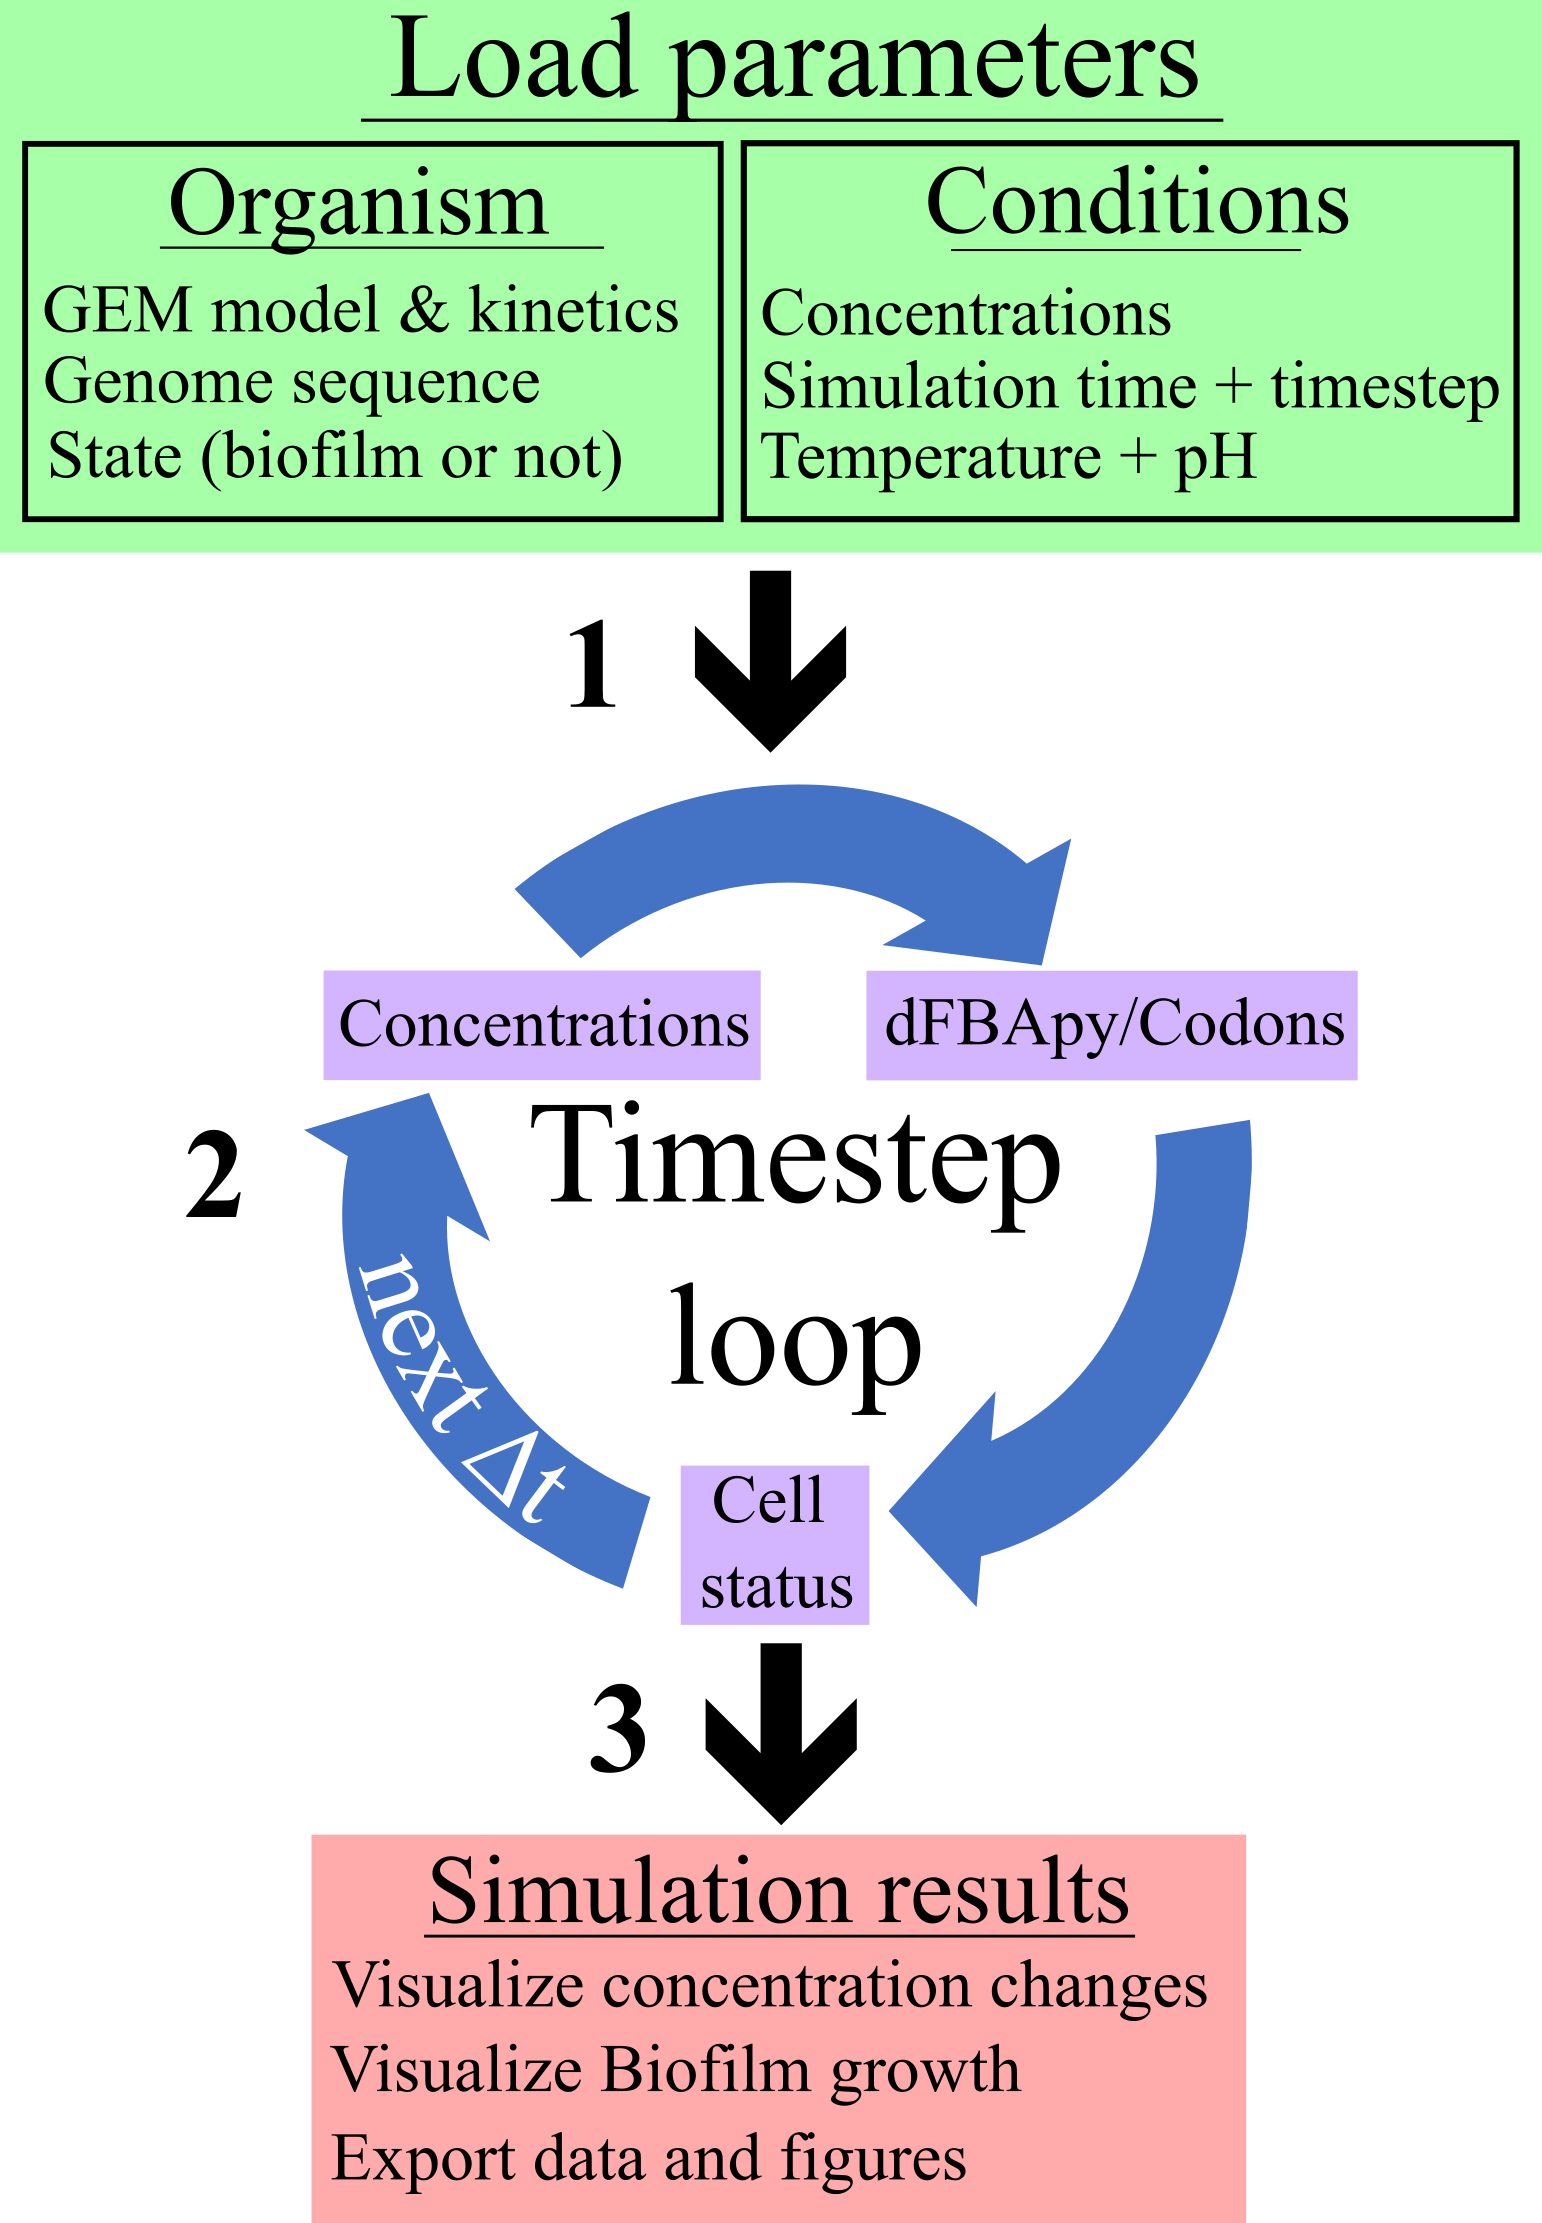
\includegraphics{images/WCMpy/wcmpy_workflow.png}
    \caption{
        The stepwise workflow of WCMpy. \textbf{Step 1} describes parameterizing the WCMpy simulation with information about the organism (e.g. the representative GEM and corresponding kinetics rate laws, the genome sequence, and the organismal state as either planktonic or sessile) and the simulation conditions (e.g. initial concentrations of the cytoplasm, the simulated time and timestep, and environmental conditions of the system). \textbf{Step 2} describes the loop that occurs with each timestep: a) dFBA and the Central Dogma are conducted based upon previous concentrations; b) the statuses of each cell and biofilm component are calculated; and c) the concentrations are updated by the reaction flux for the next timestep. \textbf{Step 3} describes processing, visualizing, and exporting the simulation results. 
    }
    \label{wcmpy_workflow}
\end{figure}

\section{Case studies}
We separately exemplify core functionality of the WCMpy workflow -- being the BiGG\_SABIO, dFBApy, and Codons modules -- in the following sections, which are available as Python Notebooks in the respective GitHub repositories.

\subsection{BiGG\_SABIO \& dFBApy}
The BiGG \textit{E. coli} core model consists only of the $95$ essential metabolic reactions for \textit{E. coli}. This model was first loaded into the BiGG\_SABIO module, where the \pyobject{parse\_data} function systematically acquired all of the data ($\approx 185 MB$) that describes the reactions of this model. The \pyobject{to\_fba} function then refined the raw data into a manageable file of kinetics data that was then directly parameterized into dFBApy and executed for an arbitrary amount of time. The results of this simulation are illustrated in Figure \ref{dfba}a, where the metabolic system re-establishes an equilibrium after the metabolism is perturbed by initial concentrations and rate law fluxes. The plotted concentrations for chemicals with defined initial concentrations are absolute concentrations, while those for chemicals without initial concentrations are only relative concentrations to the unknown initial concentration and are tagged with "(rel)" in the legend. The ability to alternatively parameterize kinetics data as an argument to the \pyobject{simulate} dFBApy function was demonstrated in Figure \ref{dfba}b by specifying only Acetate Kinase kinetic information from the full kinetic file of Figure \ref{dfba}a. 

\begin{figure}
    \centering
    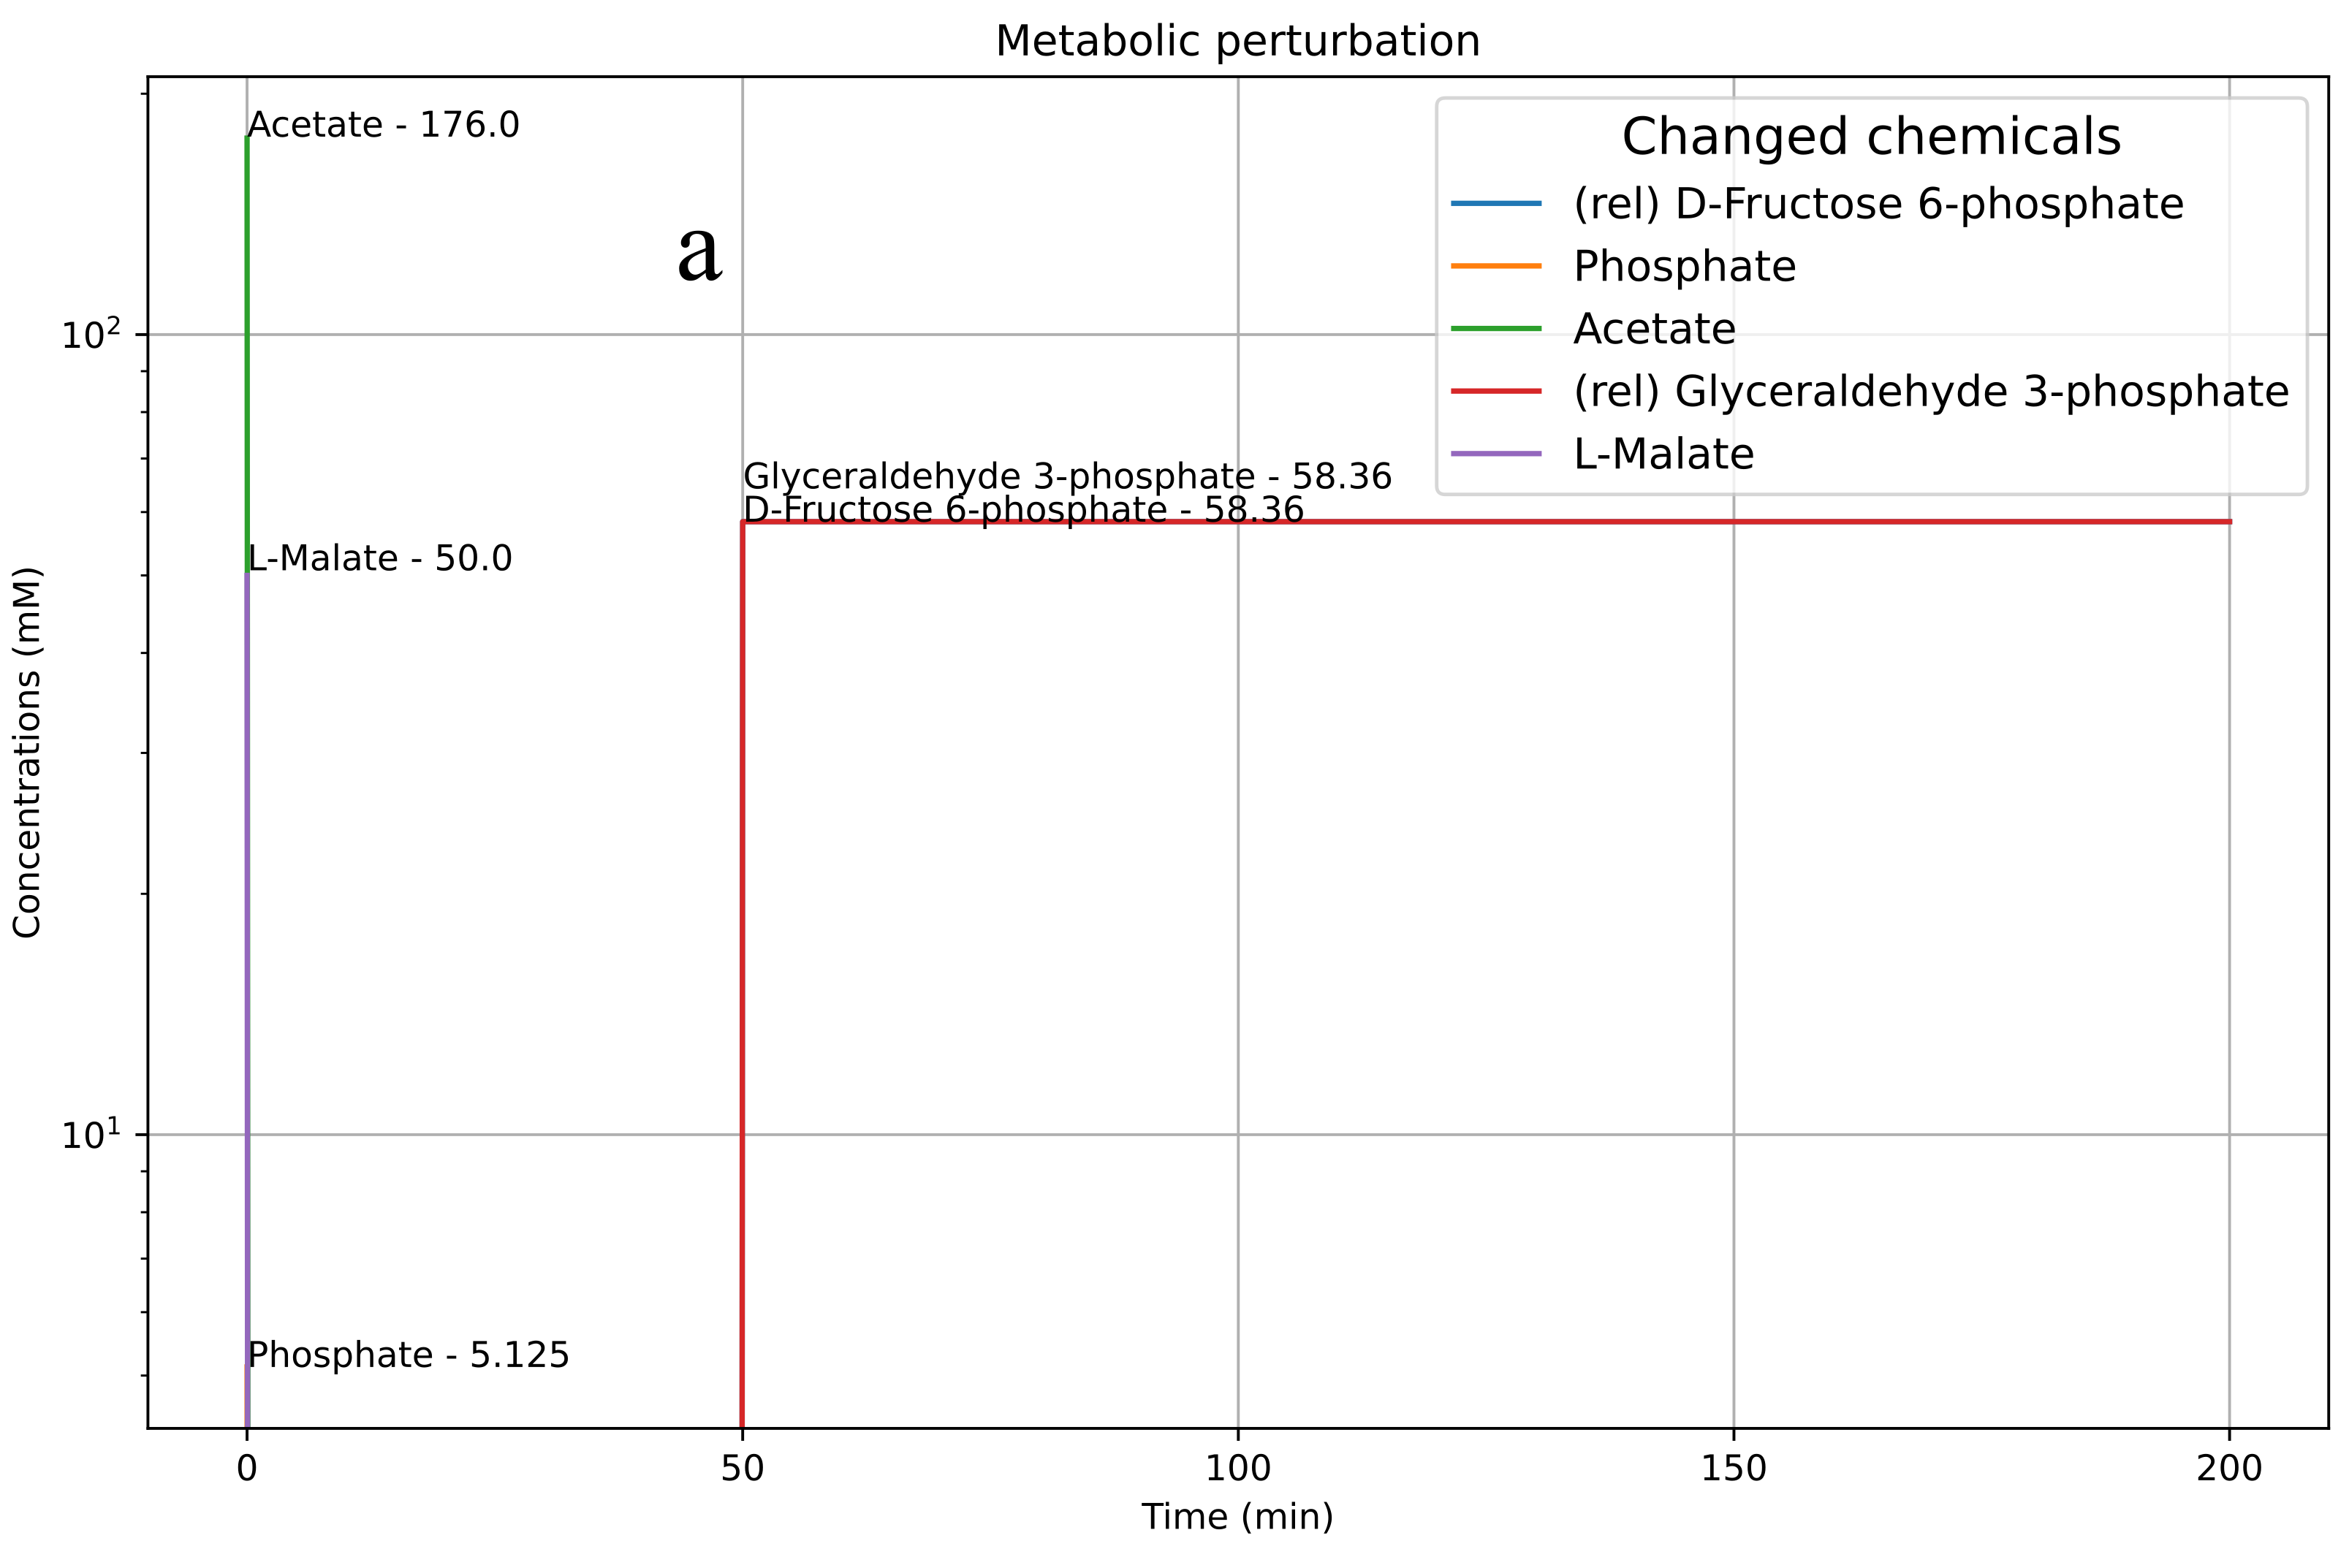
\includegraphics[width = 0.8\textwidth]{images/WCMpy/SABIO_dfba.png} \\
    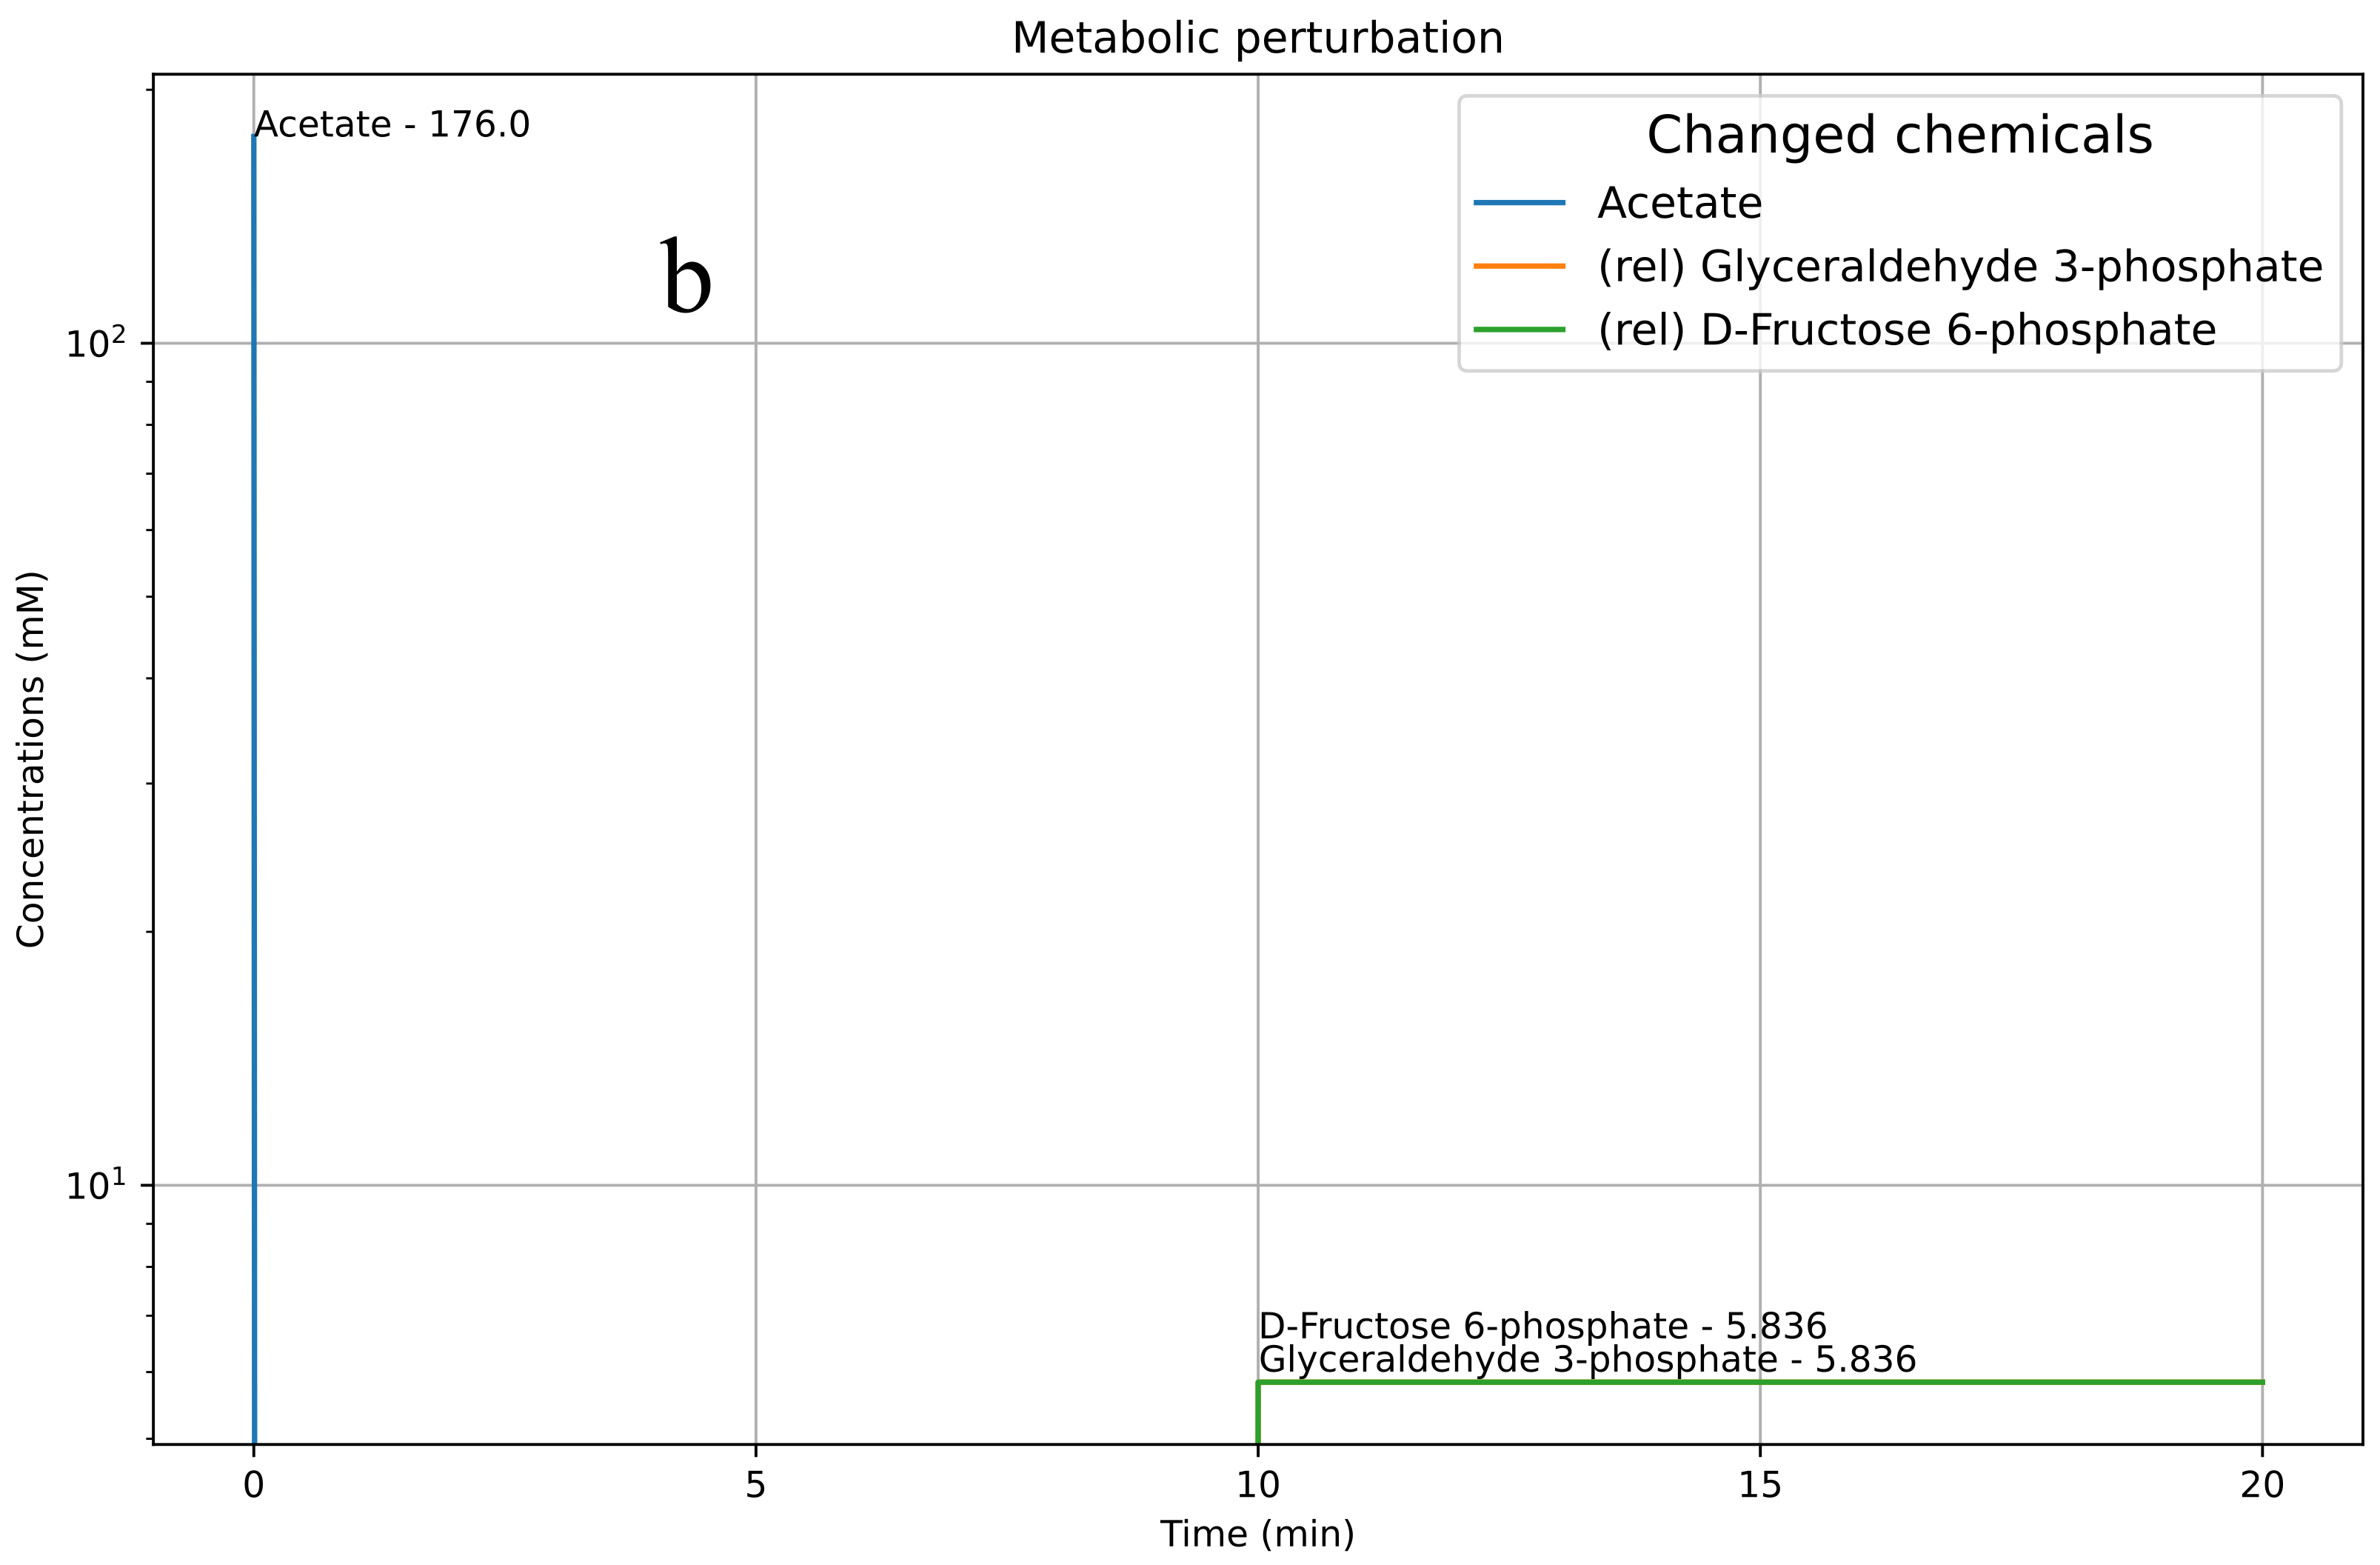
\includegraphics[width = 0.8\textwidth]{images/WCMpy/simple_argument.png}
    \caption{
        Notable concentration changes from simulating the \textit{E. coli} core BiGG model via dFBApy with a) full SABIO-RK kinetics data via the BiGG\_SABIO module and b) a single entry from the kinetics data that was passed as a function argument. Chemicals with defined initial concentrations are depicted at $t=0$, while other chemicals are labeled as relative changes "(rel)" since their initial concentrations are unknown. The metabolic consequences of these concentrations and calculated fluxes are observed over the first timestep, where equilibrium is re-established by generating D-Xylulose 5-phosphate and Alpha-D-Ribose 5 phosphate. The discrete establishment of equilibrium is the consequence of a "stiff" FBA algorithm. 
    }
    \label{dfba}
\end{figure}

\subsection{Codons}
The Central Dogma of the WC082 strain of Vancomycin-resistant \textit{S. aureus} \cite{Cong2020VancomycinFeatures}, sourced from the National Center of Biotechnology Information \cite{Haas2022StaphylococcusGenome}, was simulated through Codons. Between $[25,32]\%$ of the reported proteins, and $[65,83]\%$ of the reported peptide sequences, were perfectly translated from the 3 Mb genome -- depending upon which start codons were selected, how many open reading frames (ORFs) were translated, and whether the sense strand was translated. The translation of every possible protein, which accounts for overprinted genes, improved the accuracy to matching 41\% of proteins and 99.5\% of peptide sequences. Discrepancy between matches of entire proteins yet near 100\% matches of all peptide sequences supports that many bacterial proteins may be assembled from numerous peptides. Improvements in accuracy consequently increase a) the run time, from $1 min$ to $28 min$, and b) the proportion of false predictions, from 87\% to 97\%, for one ORF with no sense strand and for every possible protein on both strands, respectively. 

The aforementioned example with \textit{S. aureus} were contrasted with an example of the MERS (Middle-Eastern Respiratory Syndrome, $\approx 29kb$) virus \cite{Enouf2013MiddleGenome}. Slightly more of the reported proteins $\left(\frac{20}{30}\right)$ perfectly matched the translated proteins when considering all three ORFs, and 100\% of the reported proteins were perfectly translated when accounting for overprinted genes that are more common in viruses \cite{Ho2021UnconventionalTargets}, which suggests that viruses infrequently engage in peptide assembly into proteins. The sequences of the genome and the set of translated proteins were searched in the BLAST database through Codons, which were identified with 100\% certainty except for the small, ambiguous, peptides that are difficult to identify. 

\section{Discussion}
The developed suite of Python packages contributes modular tools that we postulate will foster the development of a mechanistic biofilm model, based upon a scalable WCM: WCMpy. The open-source Python community encourages collaboration, which may be particularly valuable for comprehensive projects such as WCMpy. The metabolome modules -- BiGG\_SABIO and dFBApy -- provide a conduit between a kinetics database and dFBA metabolic simulations for any organism whose metabolism is encapsulated in a BiGG-formatted GEM. These metabolic packages may individually useful to the DataNator \cite{Roth2021Datanator:Behavior} and ModelSEED \cite{Seaver2021TheMicrobes} WCM projects that are developing an improved bioinformatics resource and modelling tools, respectively. The dFBApy simulations are quantitatively consistent between the metabolic production in Figures \ref{dfba}a-b and the relative carbon input, which encourages their continued use by the community. The Codons module offers a rapid, intuitive, and practical tool for simulating the Central Dogma and investigating the genome and proteome of any organism with a known genetic sequence. These three packages advance available techniques to alleviate the noted bottlenecks -- scalable code and bioinformatics logistics -- that hinder developing mechanistic biofilm models with fundamental WCMs, which could expedite research in understanding and managing biofilms. 

\section{Author Contributions}
\begin{enumerate}
    \item \textbf{APF} - Writing and research
    \item \textbf{ESC} - Writing and research
    \item \textbf{HLB} - Writing, guidance, and funding
\end{enumerate}

\section{Acknowledgments}
The authors thank Jonathan R. Karr for his pioneering work in developing WCMs, and for providing guidance through our journey in systems biology.

% \setlength{\unitlength}{\savedunitlength}

\newpage

\begin{supplementary}

\section{Supporting Information}

\subsection{"dFBA" module}
We attempted to repurpose the "dFBA" module into a scalable and more accessible module for Windows OS. This was inhibited by the “dfba\_utils.so” file, and our attempt to replace this file with a dynamic linked library (DLL) analogue was thwarted by incompatibilities between C code in the library dependencies such as NVectors, SUNDIALS, and dlfcn and the C++ code of the DLL file. A further complication was that a few of these libraries, such as SUNDIALS, dynamically created the header files depending upon the user’s operating system; thus, a distinct DLL file would be required for each possible user architecture, which is not practical. The dFBApy module was therefore developed. 

\subsection{Thermodynamic metabolism}
We considered conducting metabolism for WCMpy via thermodynamic gradients, rather than conventional dFBA kinetics. This proposed logic is incomplete, since we migrated to the kinetic models during its development; however, the preliminary logic and calculations of the following sub-sections may still inspire the development of a thermodynamic metabolic approach.  

\subsubsection{Membrane absorption}

\begin{figure}
    \centering
    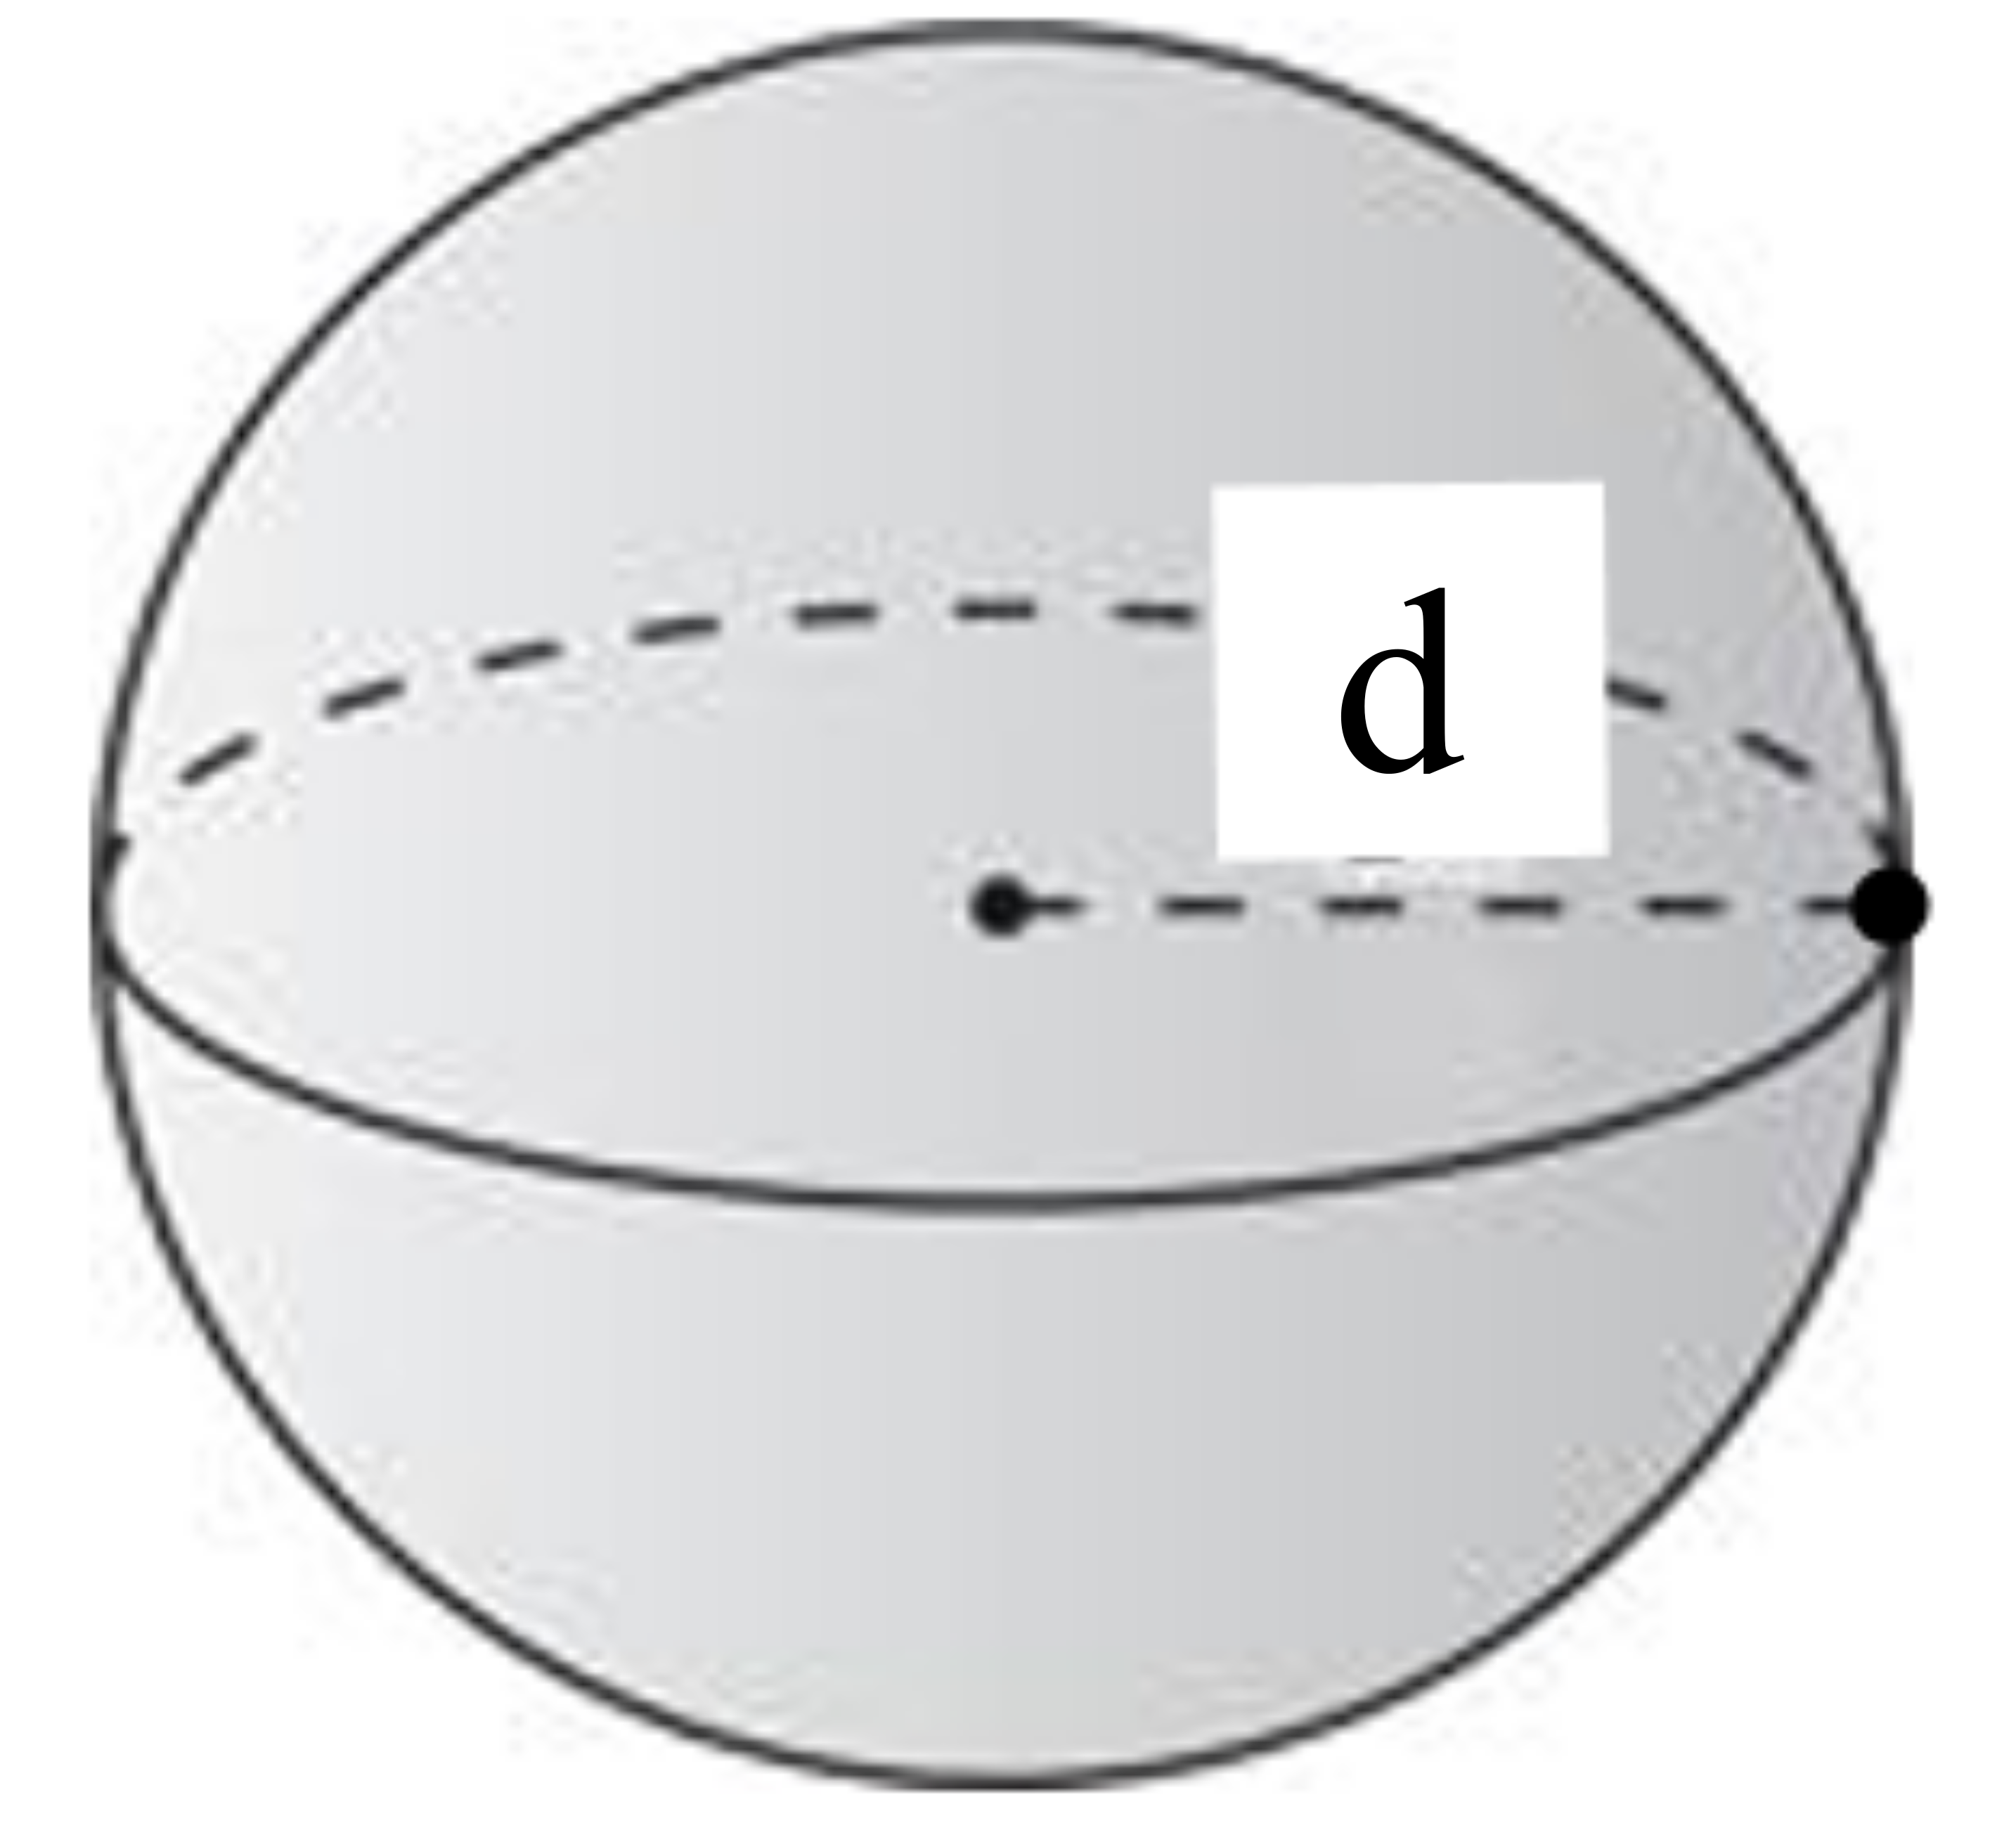
\includegraphics[width = 0.5\textwidth]{images/WCMpy/diffusion_sphere.png}
    \caption{
        A sphere where the surface area represents the location of a chemical after a timestep, which begins at the origin of the sphere, while possessing the average root-mean-squared velocity of extracellular chemicals.
    }
    \label{diffusion_sphere}
\end{figure}

\begin{figure}
    \centering
    \begin{subfigure}[b]{0.46\textwidth}
        \centering
        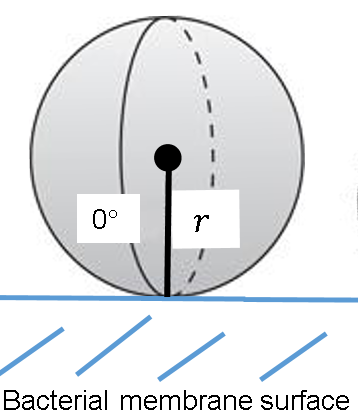
\includegraphics[width = \textwidth]{images/WCMpy/maximal_far.png}
        \caption{
            The maximal distance (d) from the bacterial membrane where a chemical can still contact the membrane with a timestep. This distance defines the thickness of the volume shell around the bacterial membrane within which chemicals may potentially be absorbed in a timestep.   
        }
    \end{subfigure}
    \hfill
    \begin{subfigure}[b]{0.47\textwidth}
        \centering
        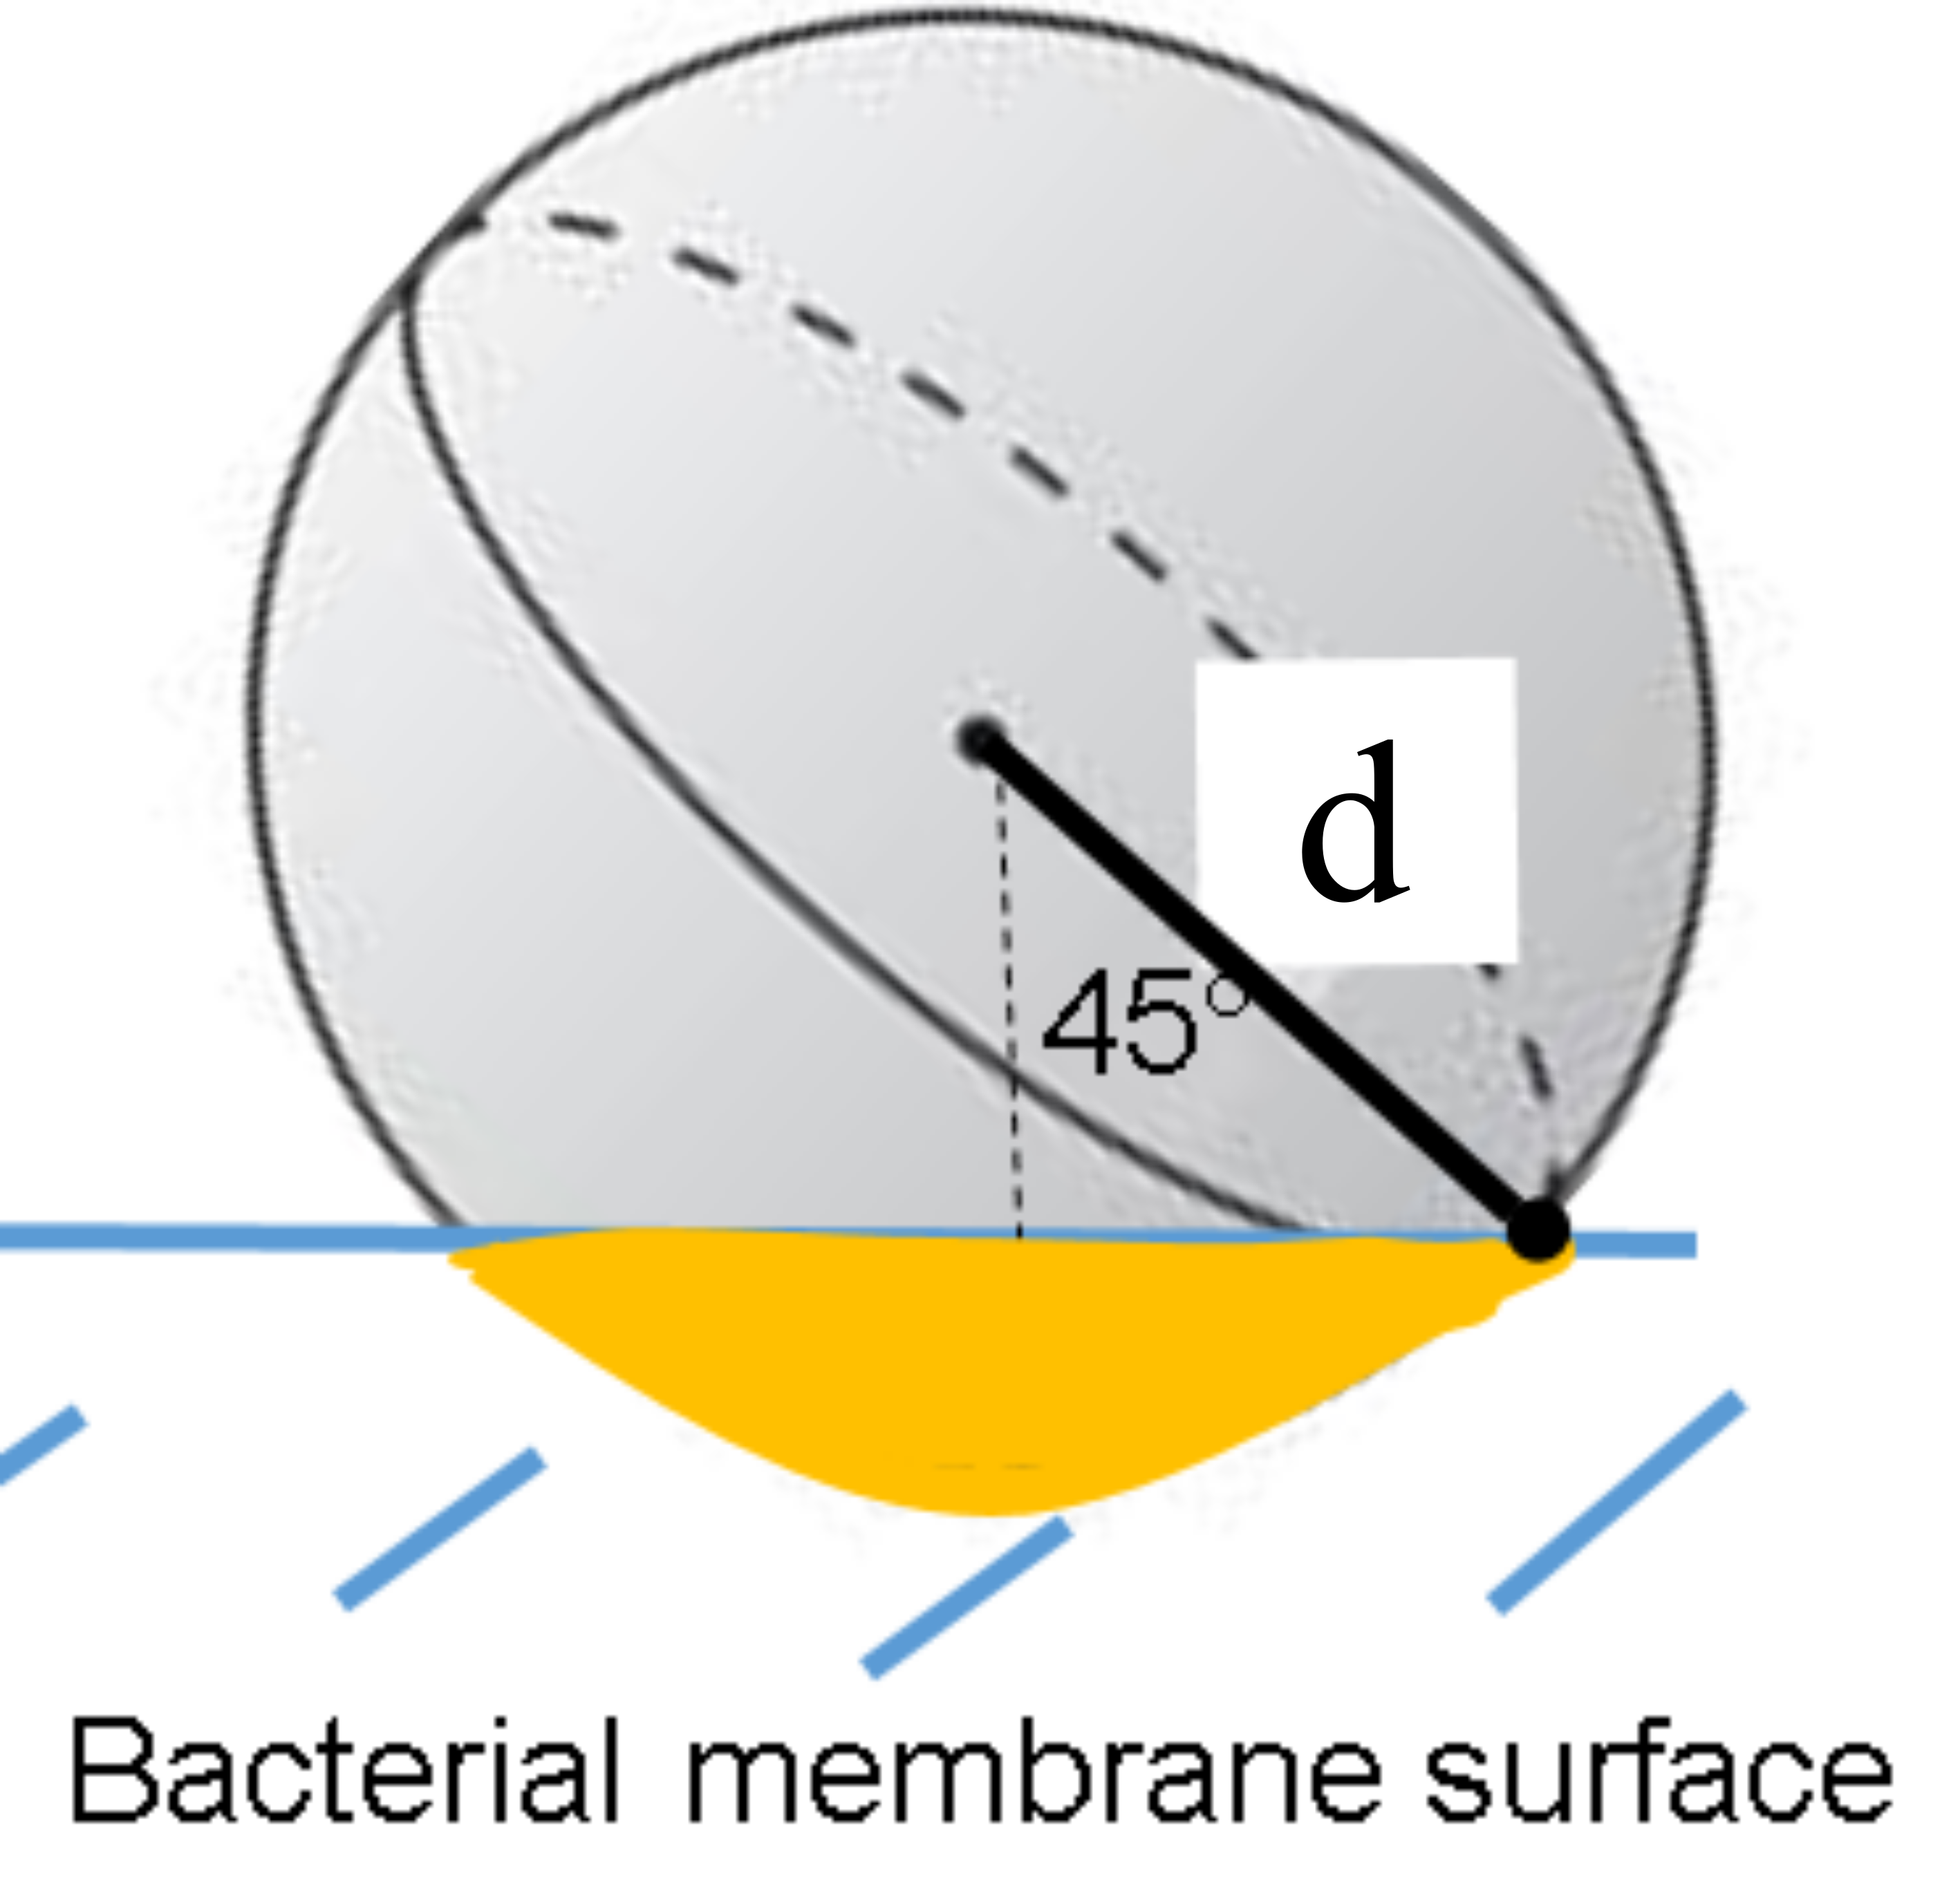
\includegraphics[width = \textwidth]{images/WCMpy/average_far.png}
        \caption{
            The average distance ($d*cos(45\degree)$) from the bacterial membrane where a chemical can still contact the membrane with a timestep. The proportion of the orange surface area and the total surface area in \cref{collision_probability} represents the probability of that a chemical within the volume shell around bacterial membrane strikes the membrane in a timestep.
        }
    \end{subfigure}
    \caption{
          Distances from the bacterial membrane where an extracellular chemical can still contact the membrane within the timestep, given a known velocity.
    }
    \label{diffusion_distances}
\end{figure}

Cellular absorption is determined by the cellular dimensions, which are calculated with each timestep. The bacterial shape is assumed to be spherical, which facilitates calculating cellular volume and surface area as a function of cellular mass $m$, via a constant density, with each timestep $\Delta t$. The quantity of absorbed chemicals is calculated as a fraction of the chemicals that exist within a distance $d$ from the bacterial membrane,
\begin{equation}
    d=\overset{\rightharpoonup}{V}_{rms}*\Delta t~.
\end{equation} 
This is the distance that a chemical, with the average root-mean-squared velocity of an extracellular chemical
\begin{equation}
    \overset{\rightharpoonup}{V}_{rms}=\sqrt{\frac{3*k_B*T}{m_{ave}}}~,
\end{equation} 		
travels in $\Delta t$, where $k_B$ is the Boltzmann constant; $T$ is the extracellular temperature in kelvins; and $m_{ave}$ is the average mass of the extracellular chemicals. The distribution of potential locations for a chemical after $\Delta t$ is conceptually represented as a sphere in Figure \ref{diffusion_sphere}, where the origin is the initial location of the chemical and the sphere surface, a $d$ distance from its origin, represents the set of possible final locations. The volumetric shell of $d$ thickness around the bacterial membrane is the volume wherein chemicals could potentially collide with the membrane and be absorbed, which is calculated
\begin{equation} \label{shell_volume}
    V_{shell}=\frac{4\pi}{3}*((r_{cell}+d)^3-r_{cell}^3)
\end{equation}
where $r_{cell}$ is the cellular radius at the start of $\Delta t$. The product of $V_{shell}$ and the extracellular chemical concentration $C_i$ of chemical $i$ 
\begin{equation} \label{shell_quantity}
    n_{shell,i}=C_i*V_{shell}
\end{equation}
yields the $n_{shell,i}$ quantity of chemical $i$ that may be potentially absorbed. The proportion $P$ of $n_{shell,i}$ that will contact the membrane is calculated as the proportion of spherical surface area in Figure \ref{diffusion_distances}b that overlaps with the membrane
\begin{equation} \label{collision_probability}
    P = \frac{SA_{membrane~collisions}}{SA_{sphere~of~possibilities}} = \frac{
    2*\pi*r_{distance~traveled}*(r_{distance~traveled}*cos(contact\_angle))
    }{
    4*\pi*r_{distance~traveled}^2
    } = \frac{(cos(45\degree))}{2} = 14.6\%~.
\end{equation}
The numerator is mathematically represented as the surface area of a conic sector of the chemical location sphere. The $contact\_angle$ of $45\degree$, between the extracellular chemical and the bacterial membrane, is the average between the maximal angle of $90\degree$ for the infinitesimally close chemical to the membrane and the minimal angle of $0\degree$ for the farthest possible chemical, which is illustrated in Figure \ref{diffusion_distances}a. The $P$ value of \cref{collision_probability} is importantly independent and constant. 

The fraction of incident $P$ chemicals that are absorbed is approximated by the thermodynamic gradient of each chemical $i$, which we propose represents the metabolic need $E_i$ of that chemical. The thermodynamic gradient is determined as the current displacement $\Pi_{R=1}^x (\frac{Q_R}{K_{eq, R}})$ -- for the $x$ number of $R$ reactions in which chemical $i$ is a reactant  -- from the optimum displacement 
\begin{equation}
    \left(\frac{Q}{K_{eq}}\right)_{optimum,i}=e^{\dfrac{\eta*n_{e^-,i}* F * E_{potential}}{R*T_{incubation}}}
\end{equation}
where $\eta$ is the total quantity of reactions in the bacterial membrane; $n_{e^-,i}$ is the average quantity of exchanged electrons in reactions where chemical $i$ is a reactant; $F$ is Faraday’s constant of electrical charge; $E_{potential}$ is the electrical potential of the bacterial membrane; $R$ is the gas constant; and $T_{incubation}$ is the incubation temperature of the simulated organism, which we presume to be indicative of the optimal thermodynamic displacement for the organism's biochemistry. The metabolic need
\begin{equation} \label{metabolic_need}
    E_i= \begin{cases}
            0, ~~\text{if} \left(\frac{Q}{K_{eq}}\right)_{optimum,i}<\Pi_{R=1}^x \left(\frac{Q_R}{K_{eq, R}}\right) \\
            \left(\frac{Q}{K_{eq}}\right)_{optimum,i}-\Pi_{R=1}^x \left(\frac{Q_R}{K_{eq, R}}\right), ~~\text{else}
        \end{cases} 
\end{equation}
is constrained to be positive, which assumes that excessive chemicals are not jettison. The absorbed quantity of chemical $i$
\begin{equation}
    n_{absorbed,i}=E_i*n_i*P*B_i~,
\end{equation}
is finally the product of its metabolic need ($E_i$ from \cref{metabolic_need}), its quantity within the volume shell ($n_i$ from \cref{shell_volume,shell_quantity}), the probability of it striking the membrane ($P$ from \cref{collision_probability}), and finally absorption hindrances that are encapsulated in $B_i$ to abstractly represent transport phenomena at the membrane that may discriminately treat different chemicals. The contribution of absorption to mass growth of the cell is calculated
\begin{equation} \label{mass_change}
    \frac{\Delta m}{\Delta t}=\sum_{i=1}^b(n_{absorbed,i}*MW_i-n_{ejected~waste,i}*MW_i)
\end{equation}
as the sum-product of the quantity of all absorbed or disposed $b$ chemicals in the metabolism and their respective molecular weights. The aggregate change in the cellular mass $\frac{\Delta m}{\Delta t}$ from \cref{mass_change} begets cellular dimensions
\begin{equation}
    r_{cell}=\left(\frac{3*\frac{m}{\delta_{cell}}}{4*\pi}\right)^{\dfrac{1}{3}}~,
\end{equation}
assuming a constant density ($\delta_{cell}$). 


\subsubsection{Chemical reactions}

Metabolic reactions are partitioned between the cytoplasm (c), the membrane (m), and the extracellular environment (e). The maximal possible quantity of chemical reactions that can proceed in the forward or backward directions is calculated $R_{max}=\left|\frac{C_i}{s}\right|$, where $C_i$ is the concentration of chemical $i$ and $s$ is the stoichiometry of chemical $i$ in reaction $R$. The maximal $R_{max}$ reaction progressions in a $\Delta t$ is attenuated $R_{actual}=R_{max}*\zeta$ by a scalar $\zeta$ that represents unreactive collisions and diffusion limitations \cite{Feynman1963ChapterDiffusion}. The $R_{actual}$ is further limited $R_{actual} = \begin{cases} R_{actual},~~if~R_{actual}<e \\ e,~~else \end{cases}$ by the quantity of enzymes that can catalyze the reaction \textit{e}. The direction of the $R_{actual}$ reactions is determined $NF = K_{eq}-Q$ by the relative difference between the current $Q$ and optimal $K_{eq}$ thermodynamic values, where $NF>0$ denotes forward reactions and $NF<0$ denotes backward reactions. The concentration change $C_i$ -- in each separate compartment -- over the timestep for chemical $i$ is calculated $\frac{dC_i}{dt}=R_{actual}*s$ as the product of the quantity of reaction progressions and the respective stoichiometry of the chemical in the reaction. The new $C_i$ is crucially used in \cref{metabolic_need} to determine the metabolic need of the chemical in the system. 

\end{supplementary}

\newpage
\startchapter{A kinetic model and API of PDI}
\label{PDIpy_chapter}

\section{Introduction}
Antibiotic resistant infections are projected to exceed cancer in annual deaths, and globally cost $10^{13}~USD$ in lost economic production, by mid-21st century \cite{ONeill2014AntimicrobialNations}. Methicillin-resistant \textit{Staphylococcus aureus} (MRSA) \cite{Song2011SpreadStudy,Borg2007PrevalenceCountries} and fluoroquinolone-resistant \textit{Salmonella} \cite{Moghnieh2018EpidemiologyLeague} are two worrisome examples of virulent pathogens that are developing resistance to the antibiotics that subdued them during the 20th century. Antimicrobial resistance (AMR) evolution can be slowed by reducing excessive and incomplete use of antibiotics for human illness and animal agriculture (which is globally the primary consumer of antibiotics \cite{VanBoeckel2017ReducingAnimals,Eggleton2020TheWorld}); however, the fundamental cause of AMR is the conventional strategy of targeting a specific microbial vulnerability. This high selectivity can mitigate off-target effects, however, it places evolutionary pressure on the pathogen to fortify the targeted biochemical vulnerability and thus become immune to the treatement. This arms race of medicinal chemists against microbial evolution must therefore be replaced with a more efficient and sustainable medical strategy, and one that ideally also avoids the persistent ecotoxicity  \cite{Thomas2001AntifoulingEffects,Niu2016RolesIrradiation,Winters1983ControlDesalination}.

\subsection{Photodynamic inactivation}

Photodynamic inactivation (PDI), which differs from photodynamic therapy (PDT) for cancer treatment \cite{Lange2019ComparisonLines} only in its application, offers an effective alternative for treating prokaryotic \cite{Hamblin2004PhotodynamicDisease} and viral \cite{Wigginton2010OxidationInactivation,Lebedeva2020TheViruses} pathogens. PDI describes a photochemical process where reactive oxygen species (ROSs) \cite{Zepp1992HydroxylReaction,Koppenol2001TheLater}, primarily singlet state oxygen ($\ce{^1O2}$, the lowest excitation state of diatomic oxygen) \cite{Ergaieg2008InvolvementPorphyrin, Allen2004IntroductionSimulations, Henze2019Multi-scaleCheckpoint, Zaman2005ComputationalMatrices,Gillespie2007StochasticKinetics}, non-selectively oxidize biological substrate \cite{Choe2006MechanismsOxidation,Frankel1980LipidOxidation}. This mechanism enables PDI to simultaneously 1) avoid resistance evolution \cite{Tavares2010AntimicrobialTreatment,Lauro2002PhotoinactivationConjugates,Pedigo2009AbsenceTherapy}; 2) treat recalcitrant biofilms \cite{Beirao2014PhotodynamicPorphyrin,Ghorbanzadeh2020ModulationModel}, where the biofilm matrix is itself oxidized by $\ce{^1O2}$; and 3) avoid ecological presistence, since $\ce{^1O2}$ has only a $\approx 100 nm$ diffusion distance and a $\approx 10^{-6} s$ lifetime \cite{Moan1984TheOxygen, Moan1990OnTissues,Rodgers1982LifetimeMeasurements} in aqueous environments. The last quality encourages the use of PDI in wastewater treatment \cite{Kohn2007AssociationOxygen,Mostafa2013SingletMatter,Jimenez-Hernandez2006SolarSensitizers} and surfaces \cite{McCoy2014PhotodynamicControl} or industrial polymers \cite{Kim2003DesignProblem} where $\ce{^1O2}$ won't leach into the environment or human consumables. 

The distinction between $\ce{^1O2}$ and triplet state oxygen ($\ce{^3O2}$, the ground conformation of diatomic oxygen) is explained by their quantum multiplicities. The singlet state, of any molecule, contains only paired electrons (couples of electrons with up and down spins) and is named after its multiplicity of $1$: from 
\begin{equation} \label{multiplicity}
    multiplicity = 2(S)+1
\end{equation}
when $S=0$. The $S$ variable in \cref{multiplicity} describes the total angular momentum of the molecule -- the sum of electron spins, where up is $+\frac{1}{2}$ and down is $-\frac{1}{2}$ -- which in the case of a singlet molecule is 0 since the complete pairing of electrons necessitates that the quantities of up and down electrons are equivalent (Figure S1). The molecular triplet state, in contrast, contains two unpaired (radical) electrons that result in a multiplicity of $3$ from $S=1$ in \cref{multiplicity}. These unpaired electrons in $\ce{^3O2}$ increase shielding of the nuclear charges \cite{Katriel1972ARule} and consequently stabilize $\ce{^3O2}$ by $0.98$ eV \cite{Jockusch2008SingletExcitation} relative to $\ce{^1O2}$ that contains lacks this shielding.

The excitation of $\ce{^3O2}$ to $\ce{^1O2}$ is controlled and augmented in PDI by photosensitizer catalysts (PSs). The PS advantageously 1) is a means of localizing oxidation, 2) is a means of controlling the timing and magnitude of excitation; and 3) is a means of generating antimicrobial concentrations of $\ce{^1O2}$ that would not occur by direct excitation $\ce{^3O2 ->[{hv}] ^1O2}$ \cite{Krasnovsky2012PhotochemicalEnvironment}, since the formal selection rules \cite{Bowen1936ForbiddenLines} describe that likely excitations are those which preserve the electronic state: i.e. ground triplet to excited triplet. The $\ce{^3O2}$ could potentially excite to another triplet state and then relax into $\ce{^1O2}$ \cite{Long2003SelectionOxygen}; nevertheless, the PS catalyst accelerates $\ce{^3O2}$ excitation through energy transfers \cite{You2018ChemicalOxygen,Schalk2008Near-infraredTetratolyl-porphyrins,Jockusch2008SingletExcitation}.

The first mechanistic step of PDI describes the ground-state PS ($\ce{^1PS}$) absorbing a photon ($hv$) and entering an excited singlet state ($\ce{^1PS^*}$), according to the selection rules. This excited state then relaxes through intersystem crossing, instead of fluorescing \cite{Kessel1982DeterminantsSpectra}, to an excited triplet state ($\ce{^3PS}$),
\begin{equation} \label{ps_excitation_steps}
    \ce{^1PS <=>[{excitation}][{fluorescence}] ^1PS^* ->[][{intersystem-crossing}] ^3PS}~.
\end{equation}
The second step describes relxation via an energy transfer from $\ce{^3PS}$ to $\ce{^3O2}$, instead of phosphorescence \cite{Mcrae1958Enhancement6}, and thereby generates $\ce{^1O2}$ while regenerating the ground-state $\ce{^1PS}$ catalyst,
\begin{equation} \label{excited_ps_steps}
    \ce{^1 PS <-[{phosphorescence}] ^3 PS ->[^3O2] ^1 PS + ^1O2}
\end{equation}
The combined efficiency of \cref{ps_excitation_steps,excited_ps_steps} is encapsulated in a quantum yield of $\ce{^1O2}$ production \cite{Bakalova2004QuantumPhotosensitizers} ($0\le \Phi_{\ce{^1O2}}\le 1 ~;~ \frac{\ce{^1O2} ~molecules ~produced}{photon ~absorbed}$). The $\ce{^3PS}$ and $\ce{^1O2}$ excited states engage in energy transfers instead of $\ce{^1PS^*}$ and $\ce{^3O2^*}$ since they have longer lifetimes as a consequence of fluorescence being more favorable than phosphorescence. The third step and final of PDI describes $\ce{^1O2}$ reacting with biological substrates through Type II oxidation mechanisms, which are concerted Schenck \cite{Prein1996TheApplications} or Alder-ene \cite{Fernandez-torquemada2012DispersionPlants} reactions that produce organic peroxides \cite{Foote1965ChemistrySelectivity}, as opposed to Type I mechanisms \cite{Bolland1949KineticsOxidation,Farmer1943TheRubber,Grynova2011RevisingAutooxidation} that only affect radical substrates \cite{Litwinienko1999DifferentialEsters}. The Type II mechanism most readily affects allylic positions of unsaturated molecules \cite{Ellison1996ThermochemistryIons,Sehon1950TheRadical}, although, saturated molecules, like those in bacterial phospholipids \cite{ODonnell1985NumericalStaphylococci}, are also oxidized by $\ce{^1O2}$,. 

\begin{figure}[t]
    \centering
    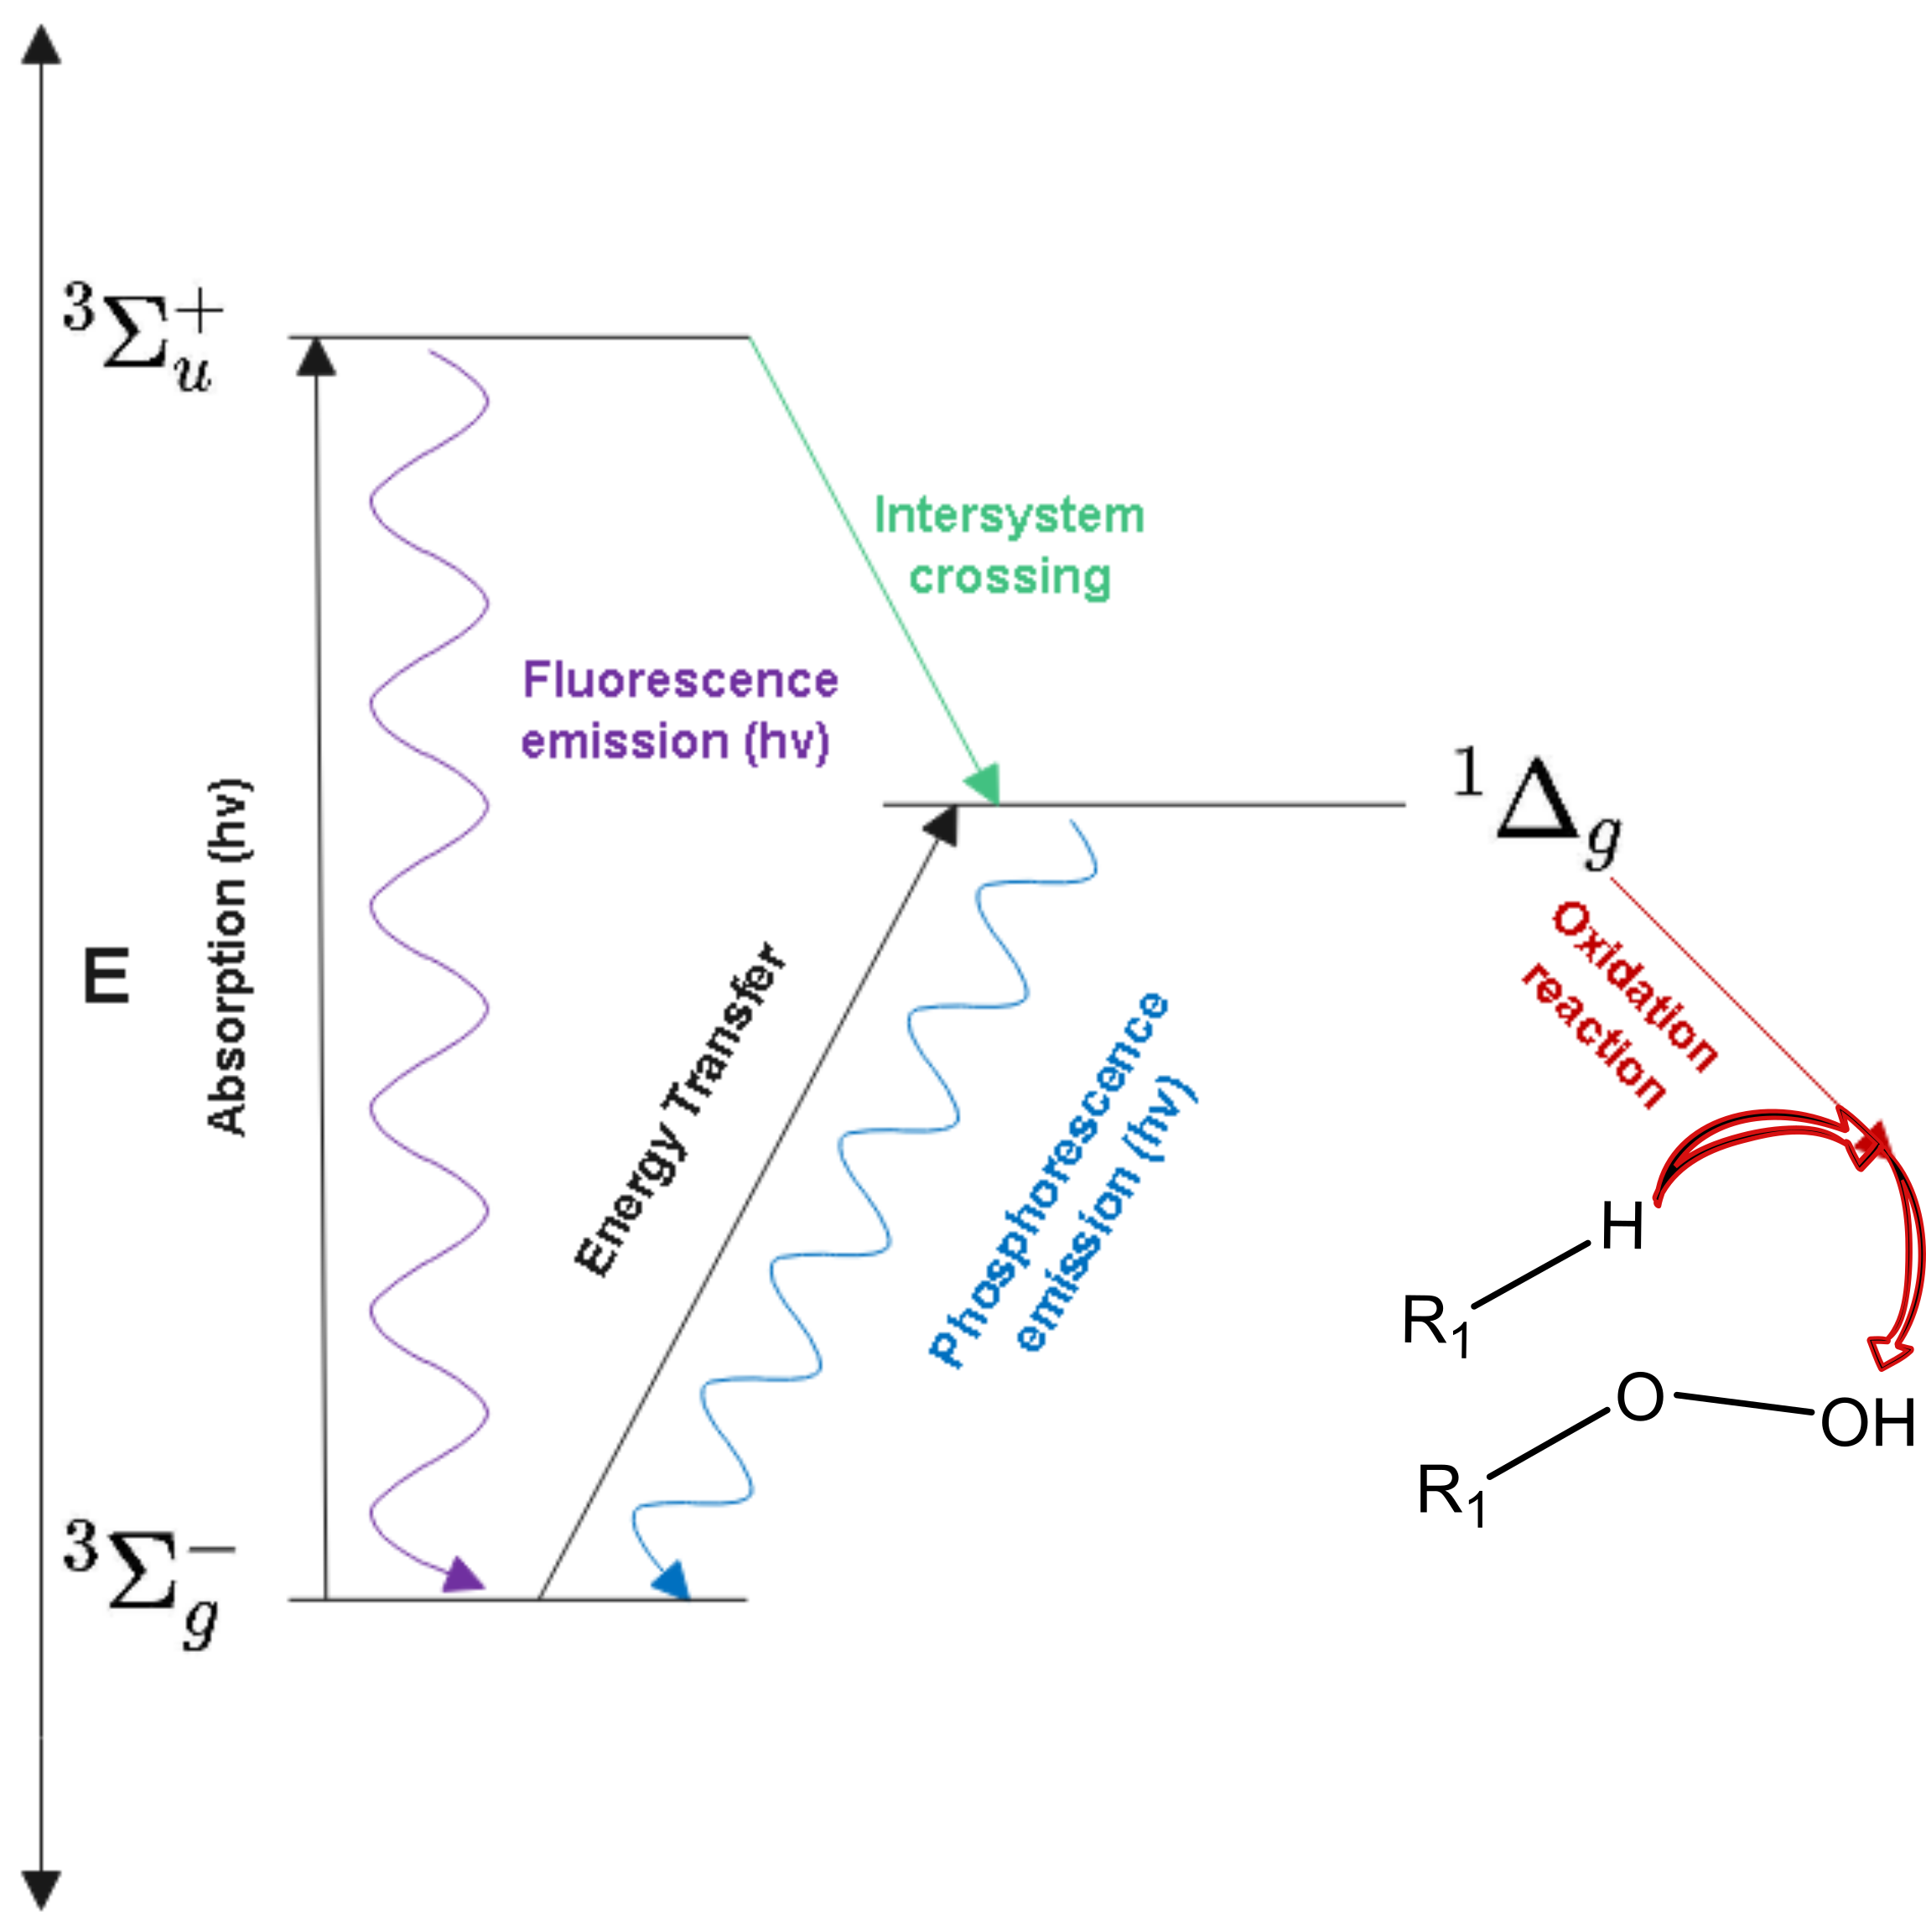
\includegraphics[width = \textwidth]{images/PDIpy/background/jablonski_diagram.png}
    \caption{
        A qualitative Jablonski energy diagram of photosensitization. The initial electronic absorption of a photon ($h\nu$) by $\ce{^3O2}$ forms a $\ce{^3O2}$* molecule, following the selection rules of excitation, which is followed with either fluorescence relaxation or an intersystem-crossing relaxation to form the reactive $\ce{^1O2}$. The singlet $\ce{^1O2}$ molecule either relaxes through phosphorescence or it reacts with an organic substrate to form a peroxide, like the illustrated hydroperoxide with a generic “R” organic group. 
    }
    \label{jablonski_diagram}
\end{figure}

\subsubsection{Photosensitizer}
The $\Phi_{\ce{^1O2}}$ efficiency is primarily dependent upon the chemical structure of the photosensitizer catalyst (PS), notwithstanding minor influence of the chemical conditions \cite{Kruk1998PhotophysicsLuminescence,Kullmann2012UltrafastBisporphyrin}. Two primary inefficiencies of PSs are its propensity to relax through fluorescence or phosphorescence, in Figure \ref{jablonski_diagram}, and to photobleach, where irradiation irreversibly compromises molecular absorptivity \cite{Bonnett2010ChemInformTherapy,Wasser1973TheMetallochlorins}. The functionality and charge of the PS should furthermore optimize its association with the targeted cells \cite{VanDerWal1997DeterminationBacteria,Dickson1989CellSurfaces} and minimize off-target oxidation \cite{Lambrechts2005PhotodynamicMice} and host toxicities \cite{Quishida2016PhotodynamicLight} in medical applications. Material applications of PDI \cite{Peddinti2018PhotodynamicThreat,Gottenbos2001AntimicrobialBacteria}, for applications in either biofouling or sterile medical surfaces, further require that the PS is amenable to permanent surface attachment in a manner that retains material properties \cite{McCoy2014PhotodynamicControl}. 

The PS finally influences the biological targets of PDI. Impermeable PSs, which cannot penetrate a cell, generally oxidize the cytoplasmic membrane \cite{Specht1990DepolarizationAction,Ehrenberg1993ElectricAlterations} instead of cytoplasmic contents \cite{Maisch2004AntibacterialDermatology}. This mechanism, which primarily affects the phospholipid fatty acids in Figure \ref{schenck_mechanism}, manifests in cell death through lysis \cite{Sahu2009AtomicColi,Bertoloni1987RoleCells} and generally affects gram-positive bacteria more than gram-negative bacteria \cite{Lauro2002PhotoinactivationConjugates,Merchat1996Meso-substitutedBacteria} since the latter possess a superficial lipopolysaccharide layer that protects the cytoplasmic membrane. Permeable PSs, by contrast, can penetrate a cell and thus generate $\ce{^1O2}$ within the cytoplasm where cytoplasmic chemicals \cite{Bagchi1979RoleAcriflavine} such as guanine nucleotides \cite{Prat1997Determination9,Devasagayam1991FormationOxygen} are fatally oxidized. This mechanism is more effective with prokaryotes than eukaryotes \cite{Quishida2016PhotodynamicLight}, since the latter have a nuclear membrane that protects DNA, particularly guanine, from oxidation \cite{Pereira2013PhotodynamicVitro}.

A narrow range of chemicals meet these criteria of an ideal PS. Semiconductors \cite{Nelson2002PhotoconductivityDioxide,Peiro2006PhotochemicalPreparations,Linsebigler1995PhotocatalysisResults}, and some amino acid residues \cite{Lippincott-schwartz2003PhotobleachingTechniques,Jin1995PhotolysisSolution}, can electrocatalytically generate $\ce{^1O2}$; however, these molecules are inefficient and/or impractical, particularly for medical applications. The most efficacious PS in nature is chlorophyll \cite{Ramel2012ChemicalPlants}, which is an organometallic porphyrinoid (Figure \ref{zinc_porphyrin}) that evolution has tuned for low rates of photobleaching and absorption of visible light -- specifically blue-violet radiation \cite{Mtangi2017ControlSplitting} via the Soret absorption band \cite{Carre1999FungicidalCerevisiae,Pereira2014InfluencePorphyrin,Ashkenazi2003PhotodynamicBacteria,Moan1986PorphyrinShGroups,Nitzan1992InactivationPorphyrins,Durantini2006PhotodynamicBacteria,Salmon-Divon2004MechanisticTetra-mesoN-methylpyridylporphine} and green-orange radiation \cite{Bertoloni2000PhotosensitizingCells} via the Q absorption band \cite{Bonnett1999PhotobleachingStudy,Jori2006PhotodynamicApplications,Gad2004TargetedMice,Zhao2019Porphyrin-basedAbsorption}. Chlorophyll, however, has not evolved traits that optimize its association with cellular targets or its compatibility with material surfaces; therefore, synthetic porphyrins \cite{Orenstein1997TheInfections,Beirao2014PhotodynamicPorphyrin,Merchat1996StudiesPorphyrins} that emulate the successful conjugated structure \cite{Huang2008Porphyrin-dithienothiopheneCells} of chlorophyll, while introducing other metal centers \cite{Mosinger1997QuantumPorphine} and functional handles  \cite{Hirao1999TheoreticalDerivatives,Wu2014BODIPY-basedSolution,Chacon1988SingletArachidonic} (e.g. Figure \ref{zinc_porphyrin}) that improve its utility in PDI \cite{Jager2016QScales,Karolczak2004PhotophysicalTetraphenylporphyrin,Mathai2007SingletTherapy}, is an appealing direction for PDI research. 

\begin{figure}
    \centering
    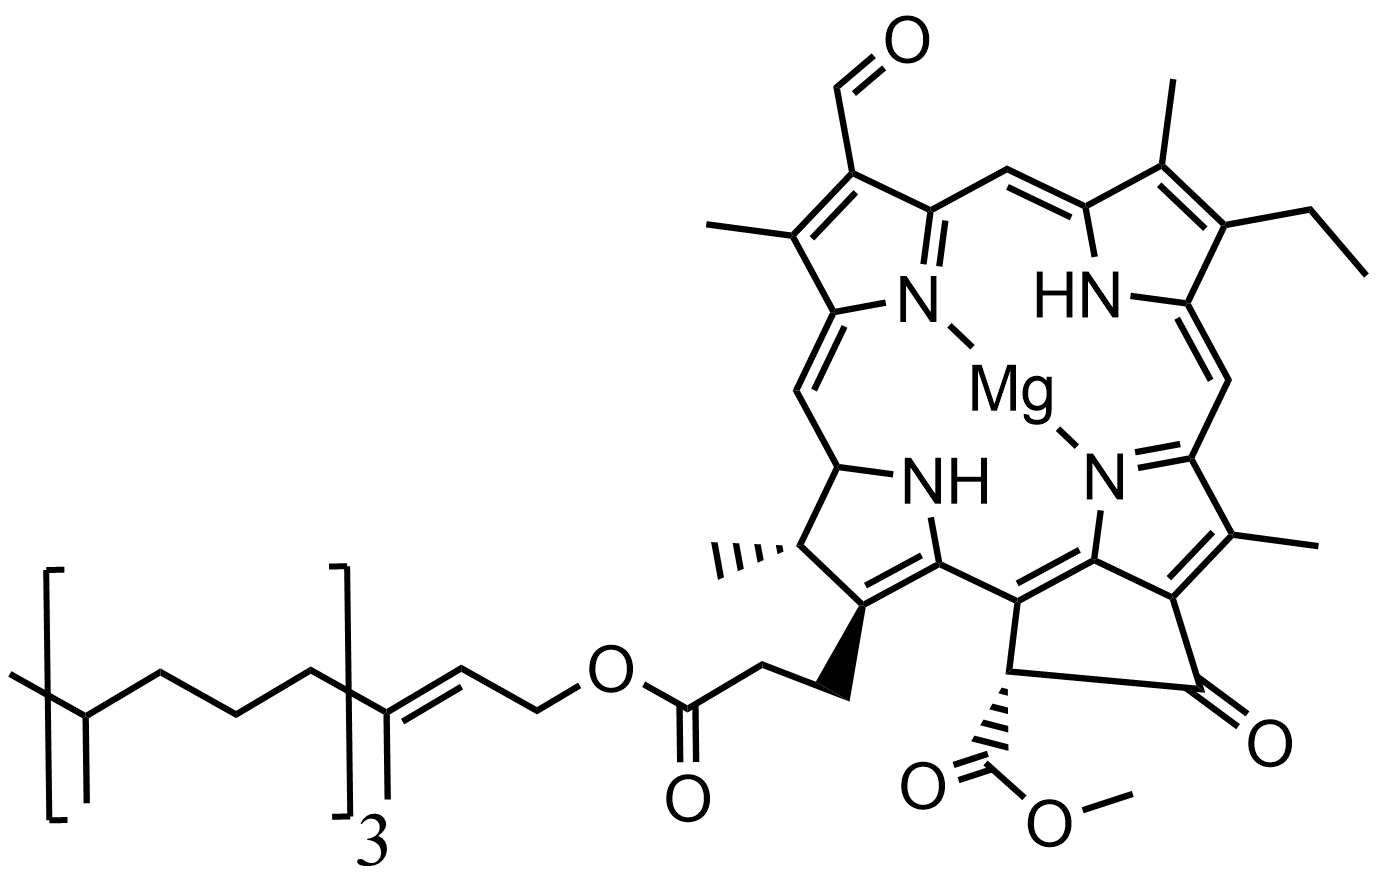
\includegraphics[width = \textwidth]{images/PDIpy/background/chlorophyll.png} \\ \midrule
    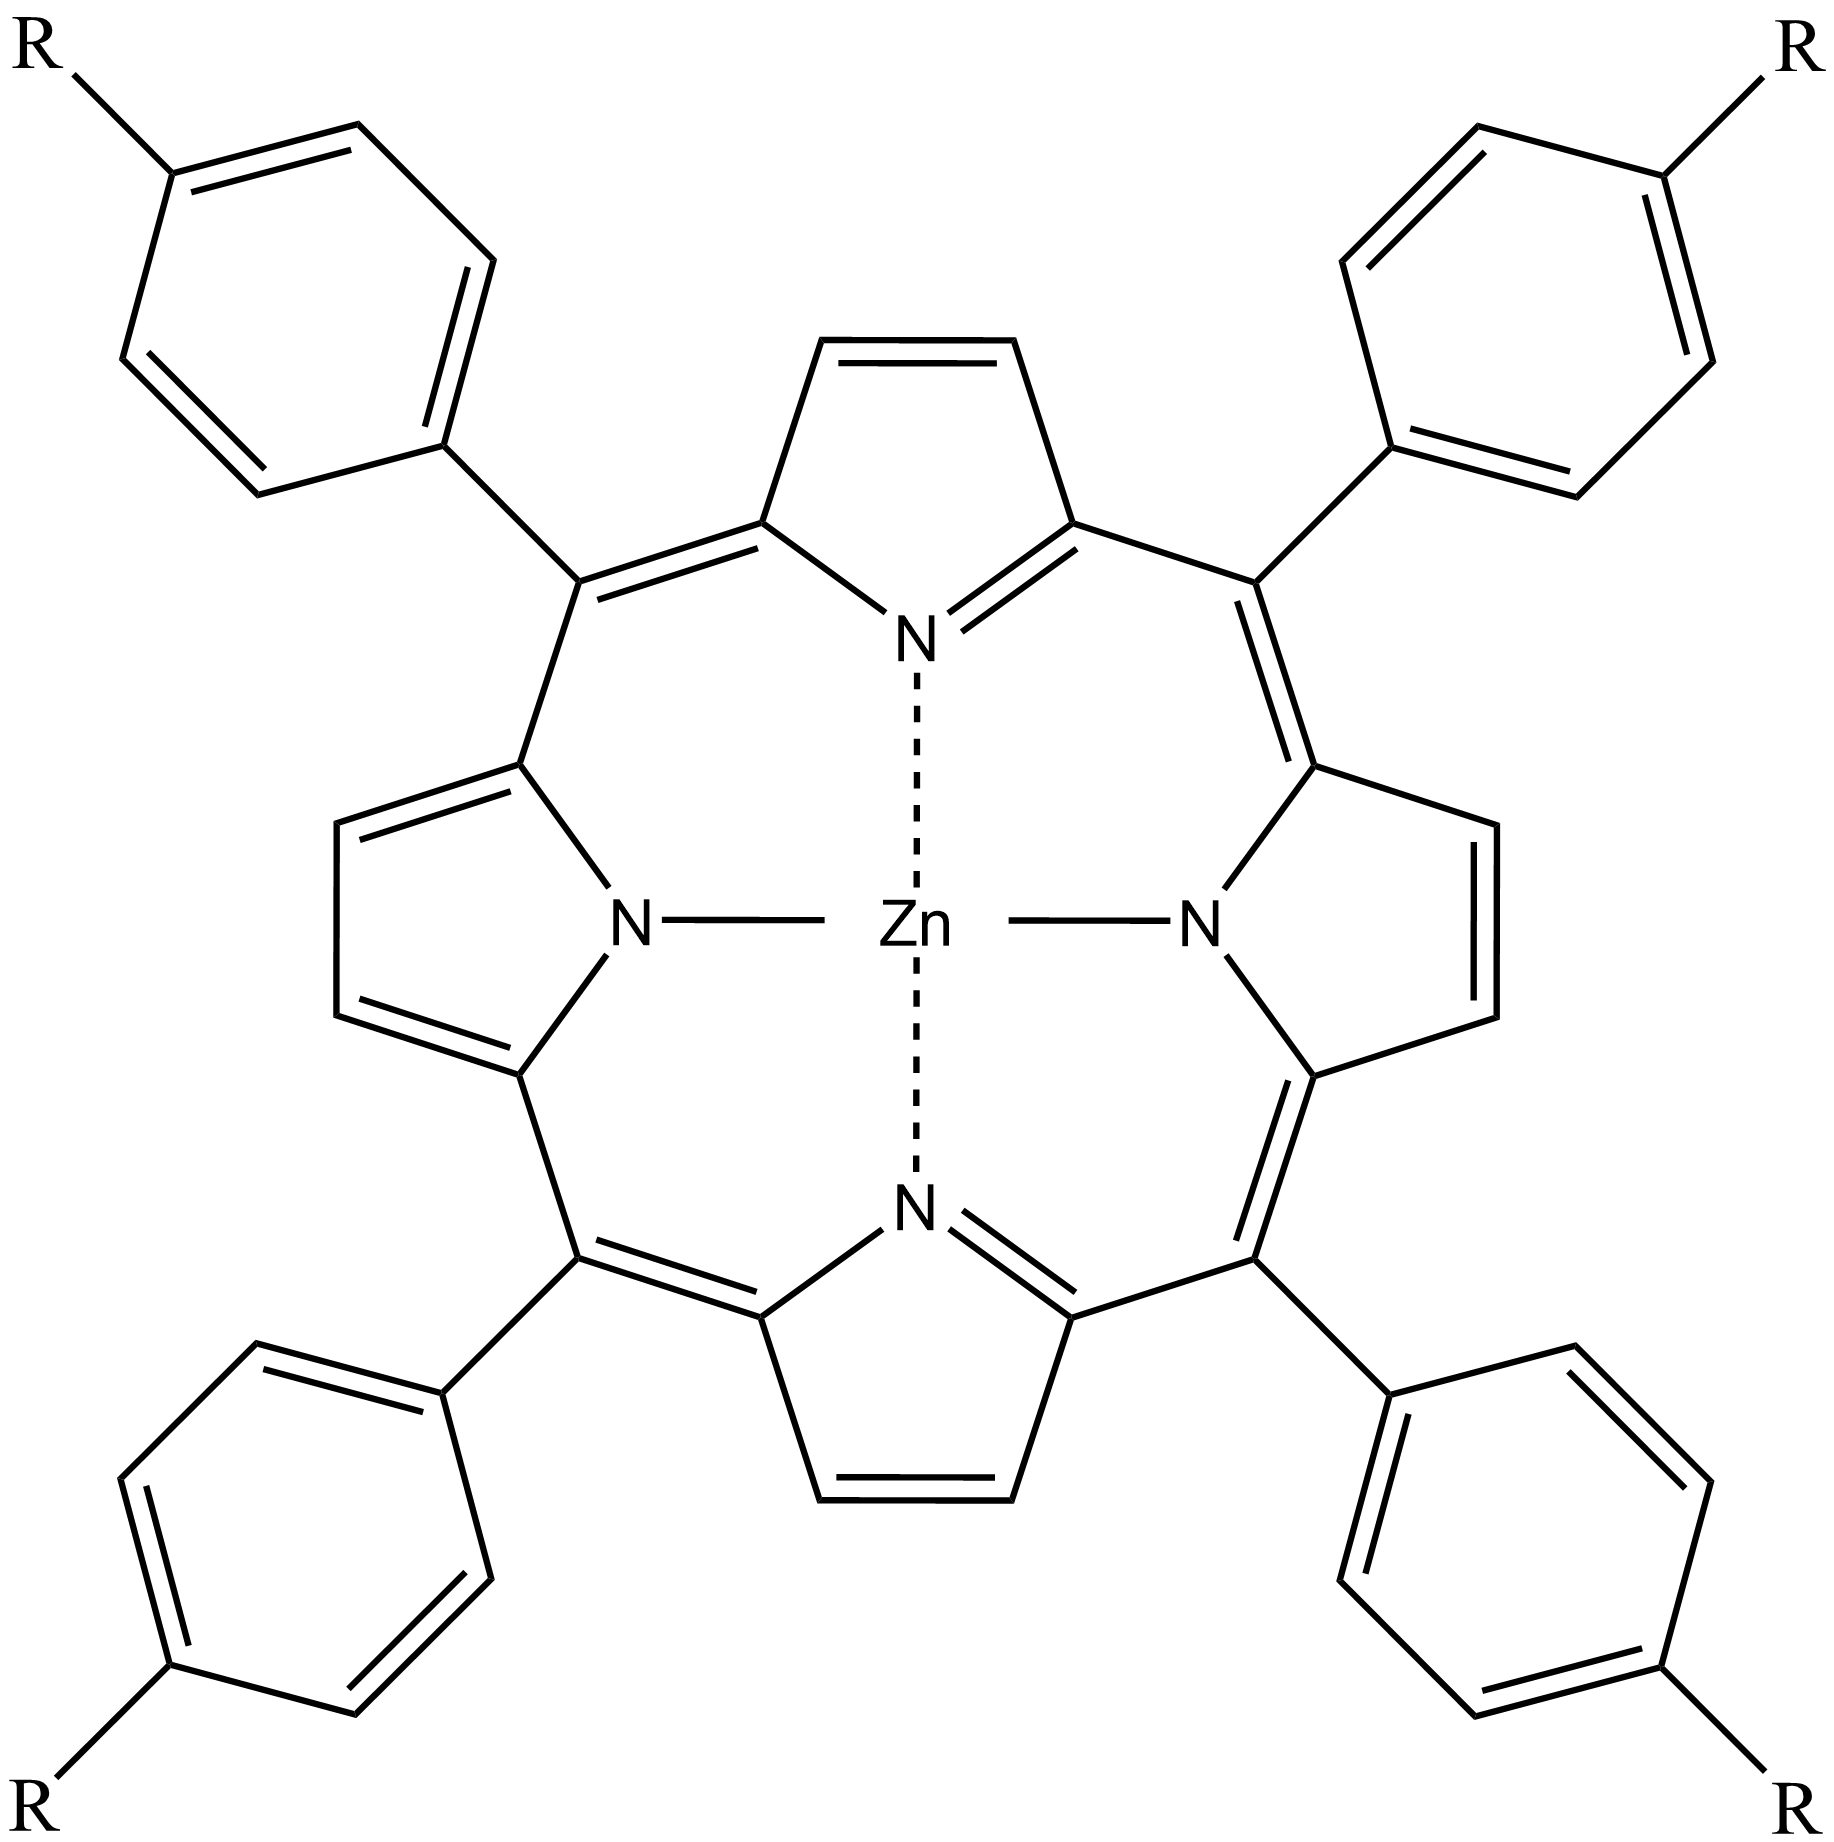
\includegraphics[width = 0.5\textwidth]{images/PDIpy/background/zinc_porphyrin.png}
    \caption{
        The chemical structure of porphyrinoid chlorophyll (top) juxtaposed with the core motif of a synthetic porphyrin analogue (bottom).
    }
    \label{zinc_porphyrin}
\end{figure}

\begin{figure}[t]
    \centering
    \includegraphics[width =0.9 \textwidth]{images/PDIpy/background/BCFA_schenck_oxidation_2.png}
    \caption{
         The Schenck reaction and associated byproduct decompositions. Step (1) depicts the concerted\cite{Foote1968PhotosensitizedOxygen} Schenck reaction. Step (2) depicts the homolytic cleavage of the hydroperoxide bond to form $\ce{OH^.}$ and an oxy radical that may enter autoxidation mechanisms. Step (3) depicts radical propagation via hydrogen abstraction to form another radical substrate and an alcohol byproduct as part of the autoxidation mechanism. Step (4) is a concerted Russell reaction\cite{Russell1957Deuterium-isotopeRadicals,Howard1968TheMechanism} between two hydroperoxides that forms a $\ce{H2O2}$, an $\alpha,\beta$-ketone, and an alcohol. The reactions of Steps (2-4) sample the wide array of possible oxidative decompositions that follow the Schenck or autoxidation mechanisms.
    }
    \label{schenck_mechanism}
\end{figure}

\subsection{PDI modeling}
Computational models of PDI that allow experimentalists, biologists and chemists alike, to explore the efficacies of different PSs and system conditions are scarce. Santos et al. \cite{Santos2020ApplicationAureus} developed a second-order polynomial to mathematically describe the inactivation of \textit{S. aureus} as a function of time at a particular wavelength and PS concentration. The predictions were demonstrated to be accurate, however, the model is bound to a narrow range of conditions, and does not permit the investigator to explore different parameters such as PS characteristics. Brasel et al. \cite{Brasel2020AnAgalactiae} developed a sigmoidal logistic model to assess the sensitivity of PDI inactivation to incident irradiance $\frac{mW}{cm^2}$ and exposure time; however, the model likewise does not permit investigations of alternative PDI systems. Finally, Sabino et al. \cite{Sabino2019InactivationTherapy} developed a Weibull power-law function from fitted inactivation data to practically predict lethal doses and the tolerance factor of a PDI system; yet, the mathematical model is limited in scope and does not describe the fundamental chemistry of PDI. 

We therefore developed a mechanistically resolved kinetic model of PDI for an impermeable PS and encapsulated into a Python API (PDIpy) that allow investigators to efficiently explore a continuum of values for numerous parameters. The means of editing and customizing the extensive list of parameters, and understanding the default values, is detailed in the API documentation. PDIpy uses Tellurium \cite{Choi2018Tellurium:Biology} to concisely construct SBML \cite{Keating2020Models}, SED-ML \cite{Waltemath2011ReproducibleLanguage}, and COMBINE OMEX \cite{Bergmann2014COMBINEProject} descriptions of the simulations and their results. These conventional formats in computational biology support transparency and reproducibility of the simulation results. The logistic (sigmoidal) Hill equation is then fitted to simulation predictions of cytoplasmic oxidation to systematically construct the inactivation plot based upon the oxidation predictions. We exemplify the model through replicating experimental studies and conducting a sensitivity analyses of key API parameters. We expect that the open-source project will foster experimental progress without expending resources, and will inspire computational biologists to refine tools for this field of medical research, towards expediting the scientific response to the looming medical crisis of antibiotic resistance. 

\section{Methods}
\subsection{Conceptual model}
PDIpy conceptually represents an experimental PDI system with a coccus (spheroid) bacterium like \textit{S. aureus}. Each simulation accepts parameters for each aspect of PDI: the light source and incident intensity; the PS absorptivity, structural dimensions, and $\frac{mol}{vol}$ or $\frac{mol}{area}$ concentration; the bacterial specie, membrane composition, and $\frac{CFU}{mL}$ for planktonic experiments; the solution dimensions; and kinetic constants for the PDI reactions. Default values for many of these parameters supplement user-defined parameters.

\subsection{Kinetic reactions}
Our model is predicated upon a set of three chemical processes that embody the essence of PDI. 1) A photoelectric interaction \cite{Wheaton2009PhotoelectricEffect} from \cref{ps_excitation_steps} occurs after $\ce{^1PS}$ is struck by a photon ($h\nu$) and undergoes intersystem crossing per to form $\ce{^3PS}$. 2) An energy transfer in \cref{excited_ps_steps} occurs from $\ce{^3PS}$ to $\ce{^3O2}$. 3) The $\ce{^1O2}$ oxidizes biological substrates, which includes both cytoplasmic phosholipids and biofilm polymeric substances, or it irreversibly disrupts PS absorptivity through photobleaching 
\begin{equation} \label{bleaching}
    \ce{^1PS -> ^1PS_{bleached}}~.
\end{equation}
A complete description of this kinetic system is represented in Table \ref{reactions_table}, and each of the reactions are each detailed in the following sub-sections.

\subsubsection{User inputs}
The PDIpy API accepts a variety of parameters that allow the user to customize almost every aspect of the PDI system. These parameters of the simulated PDI system can be provided through either a dictionary argument in the \pyobject{define\_conditions} function, or through a JSON parameter file for each category of parameters -- e.g. light, PS, bacterium, and solution space -- that elaborate the simulated system in a more reproducible and transparent manner than dictionary arguments. The complete list of accepted parameters and formats are detailed in the PDIpy documentation (\url{https://github.com/freiburgermsu/PDIpy/blob/main/README.rst}).

\begin{table}[]
    \centering
    \begin{tabular}{c|c}
        \textbf{Name} & \textbf{Reaction} \\
        \toprule
        Photoexcitation & \ce{^1PS <=> ^3PS} \\
        Photobleaching & \ce{^1PS -> ^1PS_{bleached}} \\
        Energy transfer & \ce{^3PS + ^3O2 -> ^1PS + ^1O2} \\
        Phosphorescence & \ce{^1O2 -> ^3O2} \\
        Membrane oxidation & \ce{^1O2 + FA -> oFA} \\
        EPS oxidation & \ce{^1O2 + EPS -> oEPS} \\
    \end{tabular}
    \caption{
        Each of the chemical reactions that define the PDI model of PDIpy. These reactions are individually detailed in dedicated subsections.
    }
    \label{reactions_table}
\end{table}

\subsubsection{Photoelectric}
\paragraph{PS excitation}
PDI begins with the excitation of the PS. This occurs as the combined result of an incident photon i) entering the aqueous solution, ii) striking a PS, and then iii) exciting an electron. This sequence is encapsulated in the kinetic expression
\begin{multline} \label{ps_excitation_kinetics}
    \frac{d[\ce{^3PS}]}{dt} =  k_{excitation}*\frac{photons_{PS}}{photons_{total}} \\ 
    *\Phi_{excitation}*[\ce{^1PS}] - k_{fluorescence}*[\ce{^3PS}]~. 
\end{multline}
The $k_{excitation}$ \& $k_{fluorescence}$ rate constants are estimated as the inverse of the rise and decay times for the selected PS, respectively. The approximate rise time for a porphyrin PS is $50 fs$, which is consistent with estimates of $<100 fs$ \cite{Andersson1999PhotoinducedState} and $60-90 fs$ in ethanol solvent \cite{Gurzadyan1998Time-resolvedZn-tetraphenylporphyrin} which elongates the lifetime of excited molecules relative to water. The decay time, as the S2 fluorescence \cite{Akimoto1999UltrafastPorphyrins}, and $\Phi_{excitation}$ ($\frac{PS excited}{photon absorbed}$) are approximated for a porphyrin PS as $1.5 ns$ and $\approx 0.7$ \cite{Krasnovsky2012PhotochemicalEnvironment}, respectively. The $\frac{photons_{PS}}{photons_{total}}$ \cite{Brasel2020AnAgalactiae}, which is the proportion of photons in the solution that strike a photosensitizer, is calculated through a series of steps. 1) The reported intensity of incident light from the respective light source -- i.e. either irradiance ($\frac{mW}{cm^2}$), lux ($\frac{lumen}{m^2}$), or lumens (lumens) -- is converted into $watts_{incident}$ ($\frac{J}{s}$). 2) This wattage is attenuated by the proportion of the emission spectrum $light_{incident}$ that resides within the excitation spectrum of the parameterized photosensitizer $light_{excitation}$, 
\begin{equation}
    watt_{excitation} = \frac{light_{excitation}}{light_{incident}}*watts_{incident}.
\end{equation}
3) The $watt_{excitation}$ is used to calculate the moles of incident photons that strike photosensitizers per timestep 
\begin{multline} \label{photons_per_second}
    \frac{photons_{PS}}{timestep}=\frac{<h\nu_{excitation}>}{h*c}*watts_{excitation} \\
    *\frac{second}{timestep}*reflection*scattering*\frac{1 mole}{N_A}*\frac{vol_{PS}}{vol_{total}},
\end{multline}
where $reflection \approx 96 \%$ represents the proportion of incident photons that penetrate an aqueous solution \cite{Gross1993SingletLiposomes}; and $scattering$ represents the proportion of light that reaches a specified depth \cite{RobertW.1973TheSea}, which is calculated by 
\begin{equation}
    I_z = I_0*e^{-k*z}~,
\end{equation}
where $I_z$ is the light intensity relative to the $I_0$ after depth $z$, and $k$ is the attenuation coefficient, which is $\approx 0.04~(\frac{1}{m})$ \cite{Lorenzen1972ExtinctionPhytoplankton} for clear waters. The $\frac{vol_{PS}}{vol_{total}}$ represents the volume proportion of the PS ($vol_{PS}$) -- calculated as the product of the quantity of PS molecules and the volume per molecule per its structure -- to the total volume of the solution in which the PS resides ($vol_{total}$) \cite{Santos2020ApplicationAureus}. The average excitation wavelength of the PS ($<h\nu_{excitation}>$) is calculated as the weighted average of the Soret and Q excitation bands, in proportion to their relative contribution in generating $\ce{^1O2}$ \cite{Nitzan2001PhotoinactivationWavelengths,Hoenes2020PhotoinactivationWavelength}, since this averaged wavelength simultaneously embodies contributions of both excitation bands. The resultant $\frac{photons_{PS}}{timestep}$ from \cref{photons_per_second} is then divided by the $\frac{photons_{total}}{timestep}$ to complete the kinetic expression in \cref{ps_excitation_kinetics} that calculates the excitation of PS in each timestep. 

\paragraph{Photobleaching}
The collision of a PS and a photon may alternatively disrupt the conjugated PS system and prevent further excitation, which is depicted in \cref{bleaching}. The kinetic expression 
\begin{equation} \label{bleaching_kinetics}
    \frac{d[\ce{^1PS_{bleached}}]}{dt} = k_{bleaching}*[\ce{^1PS}]*[\ce{^1O2}]~,
\end{equation}
represents this process. The $k_{bleaching}$ rate constant for the oxygen-dependent photobleaching reaction of \cref{bleaching_kinetics} -- as opposed to the oxygen-independent, first-order, photobleaching reaction \cite{Bonnett1999PhotobleachingStudy,Mang1987PhotobleachingTherapy} -- possesses a rate constant of $\approx 600 \frac{cm^2}{J*M}$ \cite{Dysart2005CalculationCells} for porphyrins, which is a function of light exposure $\frac{J}{cm^2}$.

\subsubsection{Energy Transfer}
The energy transfer from $\ce{^3PS}$ to $\ce{^3O2}$  in \cref{excited_ps_steps} is described with by the kinetics expression
\begin{equation} \label{energy_transfer_kinetics}
    \frac{d[\ce{^1O2}]}{dt} = k_{transfer}*\Phi_{transfer}*[^3PS]*[\ce{^3O2}]. 
\end{equation}
The rate constant $k_{transfer}$ is the inverse of the decay time of $\ce{^3PS}$, which for a porphyrin PS appears to be $100 ns$ in aqueous after accounting for the reported value \cite{Kupper2002KineticsOxygen} in acetone solvent that significantly increases the lifetime of excited states \cite{Spikes1992QuantumUroporphyrin}. The $\ce{^1O2}$ phosphorescence side reaction, which often emits a specific infrared wavelength that can be measured to approximate the $[\ce{^1O2}]$ \cite{Macpherson1993DirectCentres}, is kinetically represented 
\begin{equation}
    \frac{d[\ce{^3O2}]}{dt} = k_{phosphorescence}*[\ce{^1O2}]
\end{equation}
where $k_{phosphorescence}$ is a function of $\frac{CFU}{mL}$, since the $\ce{^1O2}$ lifetime is greater in biological material and thus it is proportional with the bacterial concentration in planktonic simulations \cite{Maisch2007TheBacteria}. The minimum lifetime is limited to $3.5\mu s$ for pure water \cite{Baier2005Time-resolvedCells}.

\subsubsection{Oxidation}
The oxidation reactions are the primary consumers of oxygen in the kinetic system. The simulated system, however, is assumed to possess an equilibrium between the solution and the atmosphere, which prevents the depletion of oxygen in the system. This is represented by replacing each oxygen molecule that is consumed during the oxidation of biological substrate in \cref{membrane_oxidation,EPS_oxidation}.

\paragraph{Cytoplasmic membrane} 
The oxidation of cytoplasmic phospholipids, which we approximate as fatty acid chains, is represented as an irreversible second-order reaction \cite{Watabe2007OxidationMembranes.}
\begin{equation} \label{membrane_oxidation}
    \ce{^1O2 + FA -> oFA}.
\end{equation}
and a second-order kinetic expression
\begin{equation} \label{membrane_oxidation_kinetics}
    \frac{d[oFA]}{dt} = k_{fa}*[\ce{^1O2}]*[FA]~.
\end{equation}
The rate constant $k_{fa} \approx 769 \frac{L}{g*s}$ \cite{Mukai2019KineticSolution} and the concentration of fatty acid chains in the cytoplasmic membrane is described in units of $\frac{g}{L}$, after calculating the weighted average MW of fatty acids within the membrane. 

\paragraph{Biofilm matrix} 
The oxidation of EPS is reported to be significant during PDI \cite{Beirao2014PhotodynamicPorphyrin}. This process is represented through an irreversible reaction
\begin{equation} \label{EPS_oxidation}
    \ce{^1O2 + EPS -> oEPS},
\end{equation}
which competes with \cref{membrane_oxidation} for $\ce{^1O2}$ and thereby lessens the efficacy of PDI upon biofilms relative to planktonic organisms. The oxidation of bioiflm polymers is kinetically represented  
\begin{equation} \label{EPS_oxidation_kinetics}
    \frac{d[oEPS]}{dt} = k_{EPS_{oxidation}}*[\ce{^1O2}]
\end{equation}
with an empirical rate constant that we approximated as $37.75~\frac{1}{s}$ for \textit{S. aureus}, and an initial concentration of EPS that is $9x$ greater than the cellular mass, in proportion to mass distributions of biofilms \cite{Flemming2010TheMatrix}.

\subsection{Inactivation fitting}

Simulation results of chemical concentrations over time are processed into predictions of bacterial inactivation through a series of mathematical steps. 1) The proportion of oxidized substrate
\begin{equation} \label{oxidation_proportion}
    ox_{proportion} = \frac{[oFA]}{[oFA]+[FA]}
\end{equation}
is fitted to a sigmoidal curve, similar to other models \cite{Xiong1999AInactivation}. We used the signmoidal Hill-equation \cite{Gesztelyi2012ThePharmacology} as a biochemical kinetic model that derives from mass-action kinetics similar to the Michaelis-Menten kinetic model, however, a fitting module for the Hill-equation did not exist; hence, the HillFit Python module was developed with a variation of the Hill-equation \cite{Inoue2016OscillationActivation} 
\begin{equation} \label{hill_eq}
    y=bottom+\frac{(top-bottom)*x^n}{EC50^n+x^n}~,
\end{equation}
that improves its fit to data, to fit the oxidation data from PDIpy simulations. The regression parameters from the fitted Hill equation are then systematically adjusted to construct an inactivation plot that replicates experimental results while preserving the underlying Hill-equation relationship. These parameter adjustments are presented in Table \ref{hill_parameters} for both simulations of planktonic and biofilm bacteria, since biofilms factors such as impaired diffusion that are not explicitly accounted in our kinetic model and thus must be compensated through other means. The top parameter of \cref{hill_eq} is adjusted asymptotically to a limit that follows an subtly different empirical expression for planktonic $1-10^{-\Omega}$ than biofilm $1-10^{-0.7-\Omega }$ simulations, where $\Omega = wattage^{\frac{1}{5}}-log10(1-final_{oxidation\_proportion})$. This top limit is empirically determined to manifest in the log-inactivation predictions being 1-2 greater than the log-oxidation from \cref{oxidation_proportion}, which embodies our assumption -- and an implicit observation in experimental studies -- that $1-10\%$ of membrane phospholipids must experience oxidation for the cell to lyse. 

\begin{table}[]
    \centering
    \begin{tabular}{l|c|c}
        \textbf{Bacterial state} & \textbf{Hill parameter} & \textbf{Adjustment} \\
        \multirow{2}{}{Planktonic} & EC50 & -76\% \\
         & nH & +100\% \\
         \midrule
         \multirow{2}{}{Biofilm} & EC50 & -65\% \\
         & nH & +120\% \\
    \end{tabular}
    \caption{
        The Hill parameters adjustments that are enacted to create the inactivation plot for both planktonic and biofilm systems. 
    }
    \label{hill_parameters}
\end{table}

% \subsubsection{Cross-linked systems}

% \paragraph{iPDIpy}
% The PDIpy API is graphically interactive through a user interface iPDIpy, which is depicted in Figure \ref{}. This interface provides a convenient means for parameterizing a PDIpy simulation, exporting and importing sets of parameters, parsing the processed simulation data, viewing error messages and calculated values, viewing the output figure of bacterial reduction over time, and parsing the processed data through a build-in function. The iPDIpy version of PDIpy is downloadable from our GitHub repository.

% \begin{figure}
%     \centering
%     \includegraphics{}
%     \caption{
%         The left pane of the GUI will contain command buttons like restarting the simulation or export results, while the right pane will edit the simulation data and or bacterial qualities/species.
%     }
%     \label{iPDIpy_interface}
% \end{figure}


\section{Case Studies}
A PDI experiment from literature that thoroughly described its expeirmental procedure was parameterized in PDIpy to compare the predicted results with the reported results. These comparisons in the following sections all pertain to \textit{S. aureus}, which is a model coccus bacterium that is abundantly described in studies of PDI and AMR infectants as MRSA.

% \subsection{Cross-linked PS}
% Experimental data from our lab with cross-linked PSs (unpublished) was parameterized, in Table \ref{}, into PDIpy. The predicted reduction curve over time in Figure \ref{} agreed with the experimental data at the measured time of 6 hours and 98\% reduction, which supports that the software yields accurate predictions. 

% \paragraph{}
% .

\subsection{Solution PS}

\paragraph{Beirao et al.\cite{Beirao2014PhotodynamicPorphyrin}}
This paper experimentally examines the efficacy of a dissolved PS, over a range of concentrations, against both planktonic and sessile states. The ample experimental details were parameterized into PDIpy, and the predicted log-inactivation was contrasted with the reported log-inactivation at various times, concentrations, and bacterial states in Table \ref{beirao_et_al_data}. The predicted log-oxidation and log-inactivation for a few of the simulated conditions from the study are plotted in Figure \ref{beirao_et_al}, with the respective regression plots from fitting the Hill-equation to the log-oxidation results in Figure \ref{hill_regression}. The very precise fitting of the data -- $R^2 > 0.996$ -- supports that our kinetic model of PDI fundamentally recreates the biochemical relationship that is predicted by the Hill model of kinetics.

\begin{table}[h]
    \centering
    \begin{tabular}{c|c|c|c|c|c}
        Bacterial & [PS] & Inactivation & Reported & Predicted & \multirow{2}{1.2cm}{\%-error}\\
        state & ($\mu m$) & (-log10) & (min) & (min) & \\
        \toprule
        \multirow{3}{1.5cm}{planktonic} & 5 & 7.6 & 51 & 117 & 119\\
        & 10 & 7.6 & 51 & 36 & -29\\
        & 20 & 7.6 & 42 & 12 & -71\\
        \midrule
        \multirow{3}{1.5cm}{sessile} & 5 & 3.6 & 390 & 566 & 45\\
        & 10 & 5 & 390 & 310 & -20\\
        & 20 & 6.3 & 390 & 247 & -37\\
        \bottomrule
    \end{tabular}
    \caption{
        A quantitative comparison of published inactivation data, with both planktonic and sessile, \textit{S. aureus}, with predictions from PDIpy. The \%-error for each prediction is provided in the table as a metric of accuracy
    }
    \label{beirao_et_al_data}
\end{table}

\begin{figure}
    \centering
    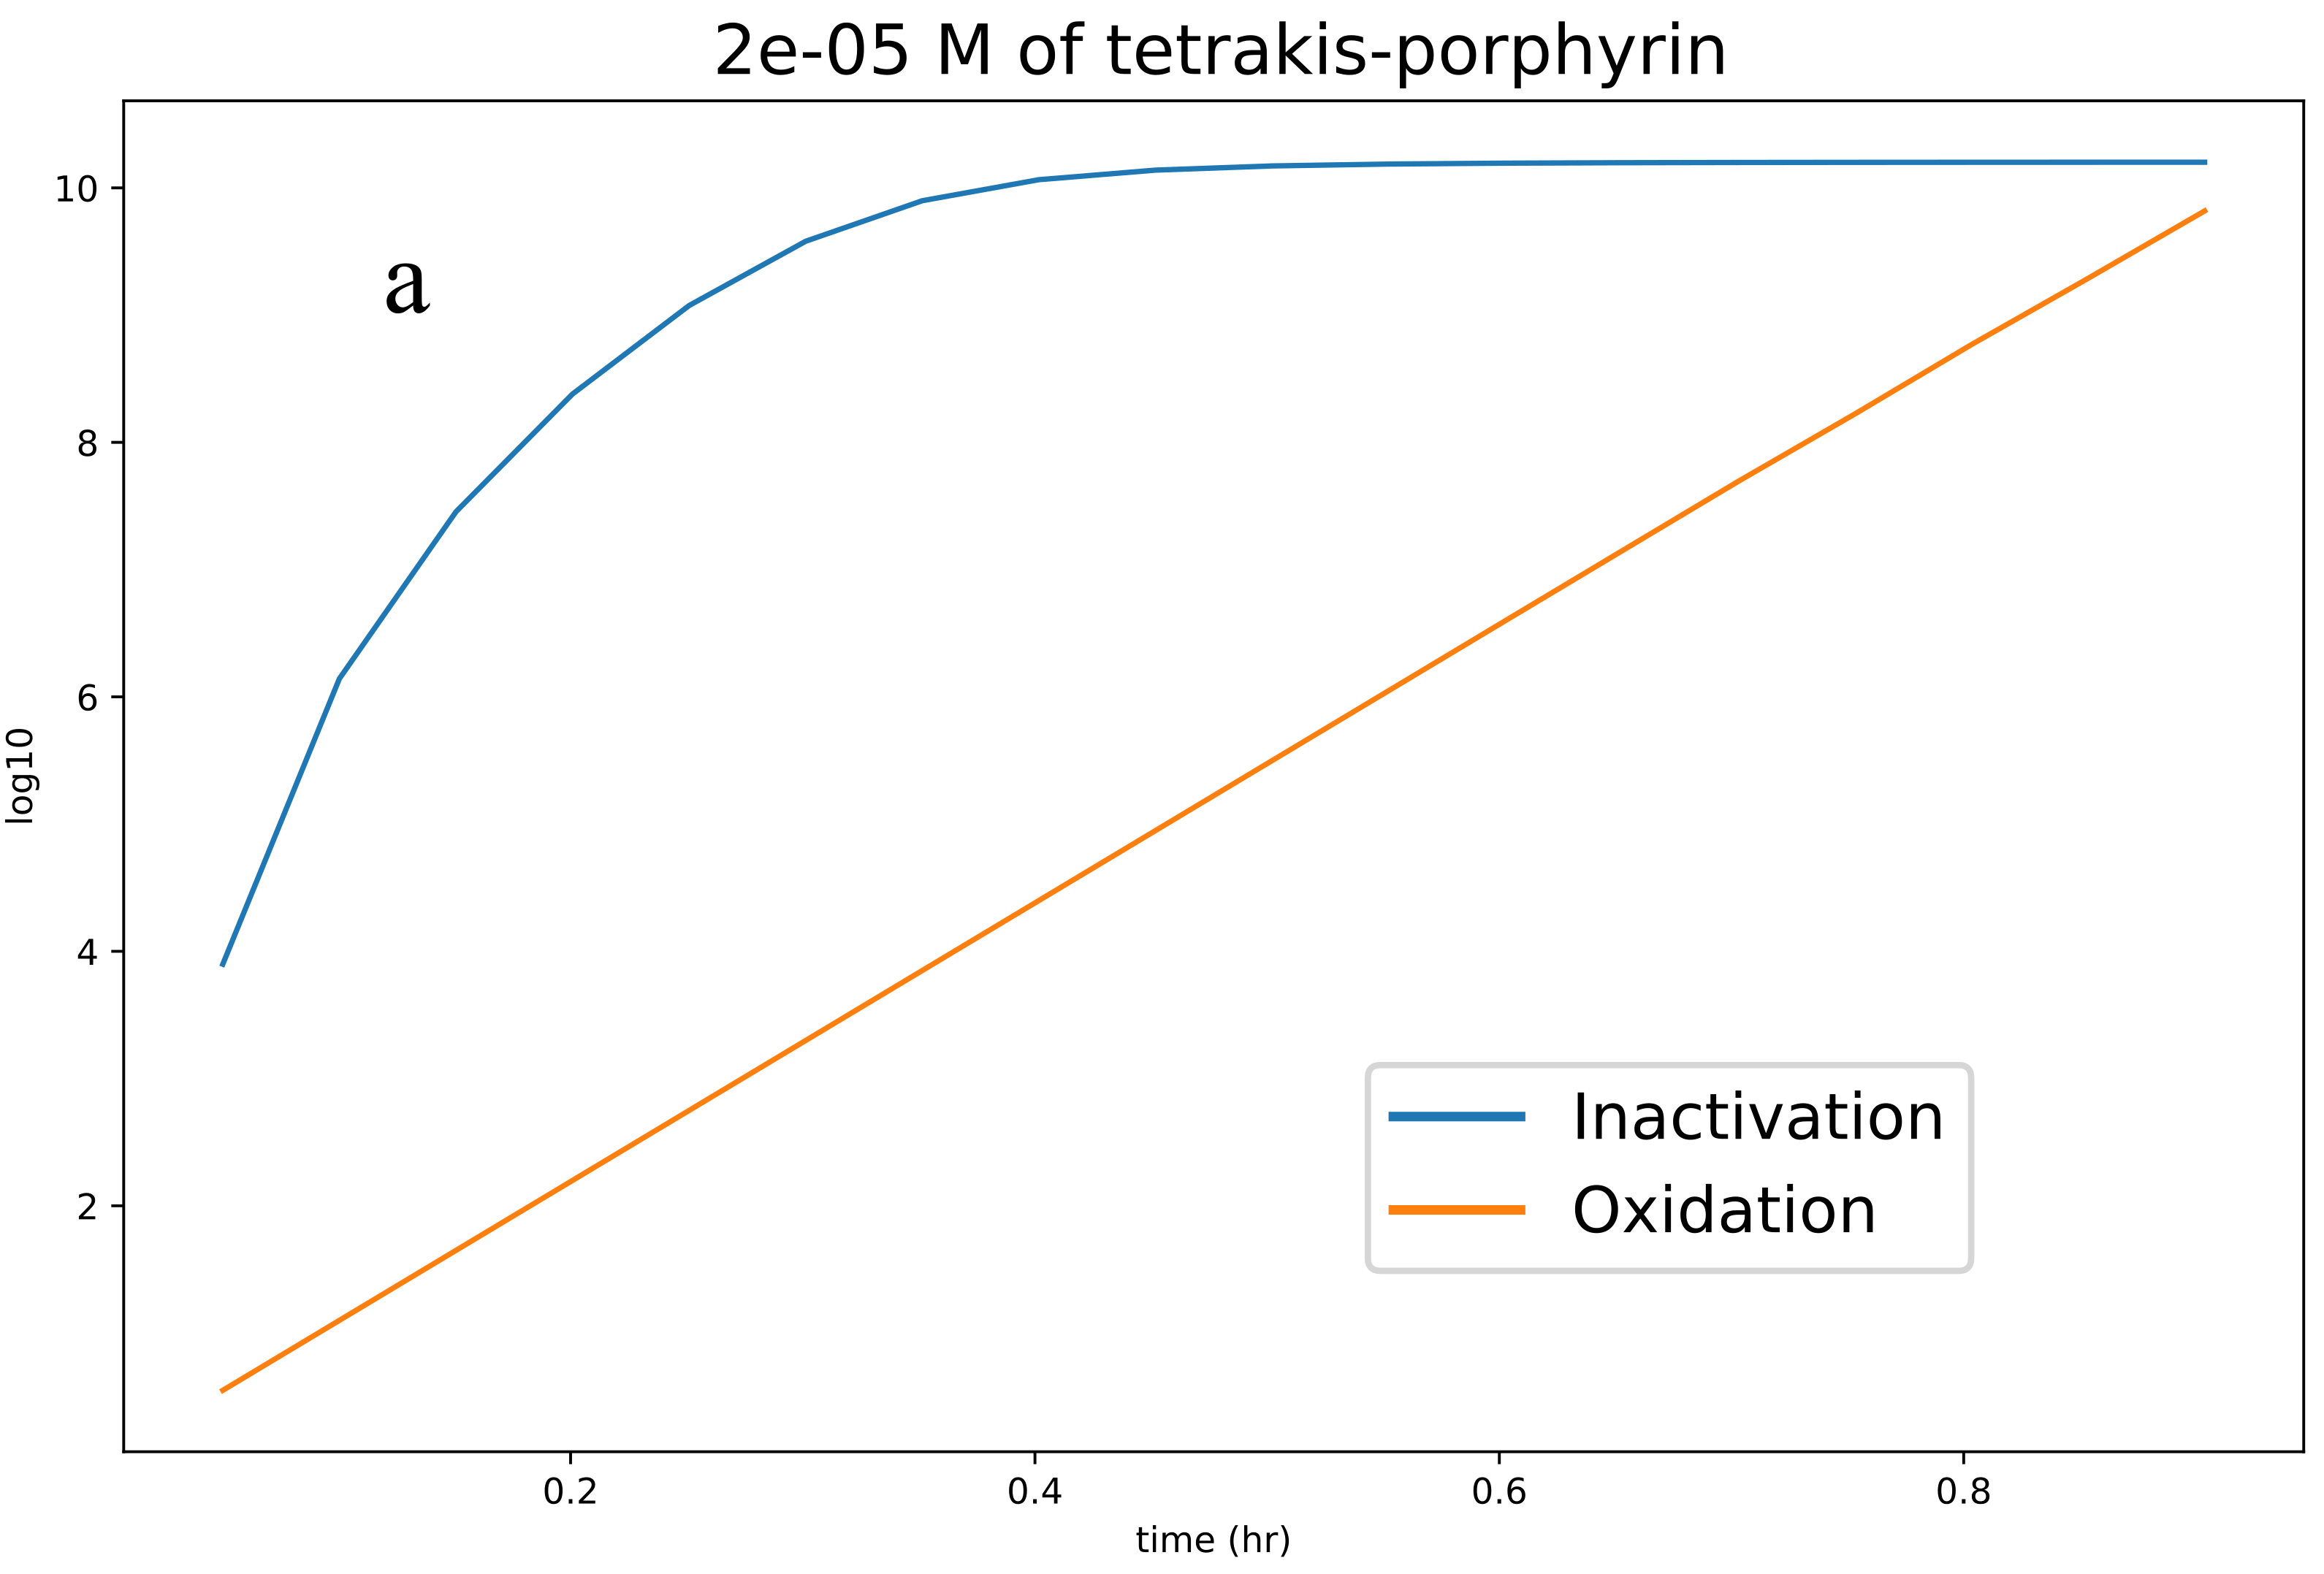
\includegraphics[width = 0.9\textwidth]{images/PDIpy/examples/20uM.png}
    \vspace{5mm}
    \midrule
    \vspace{5mm}
    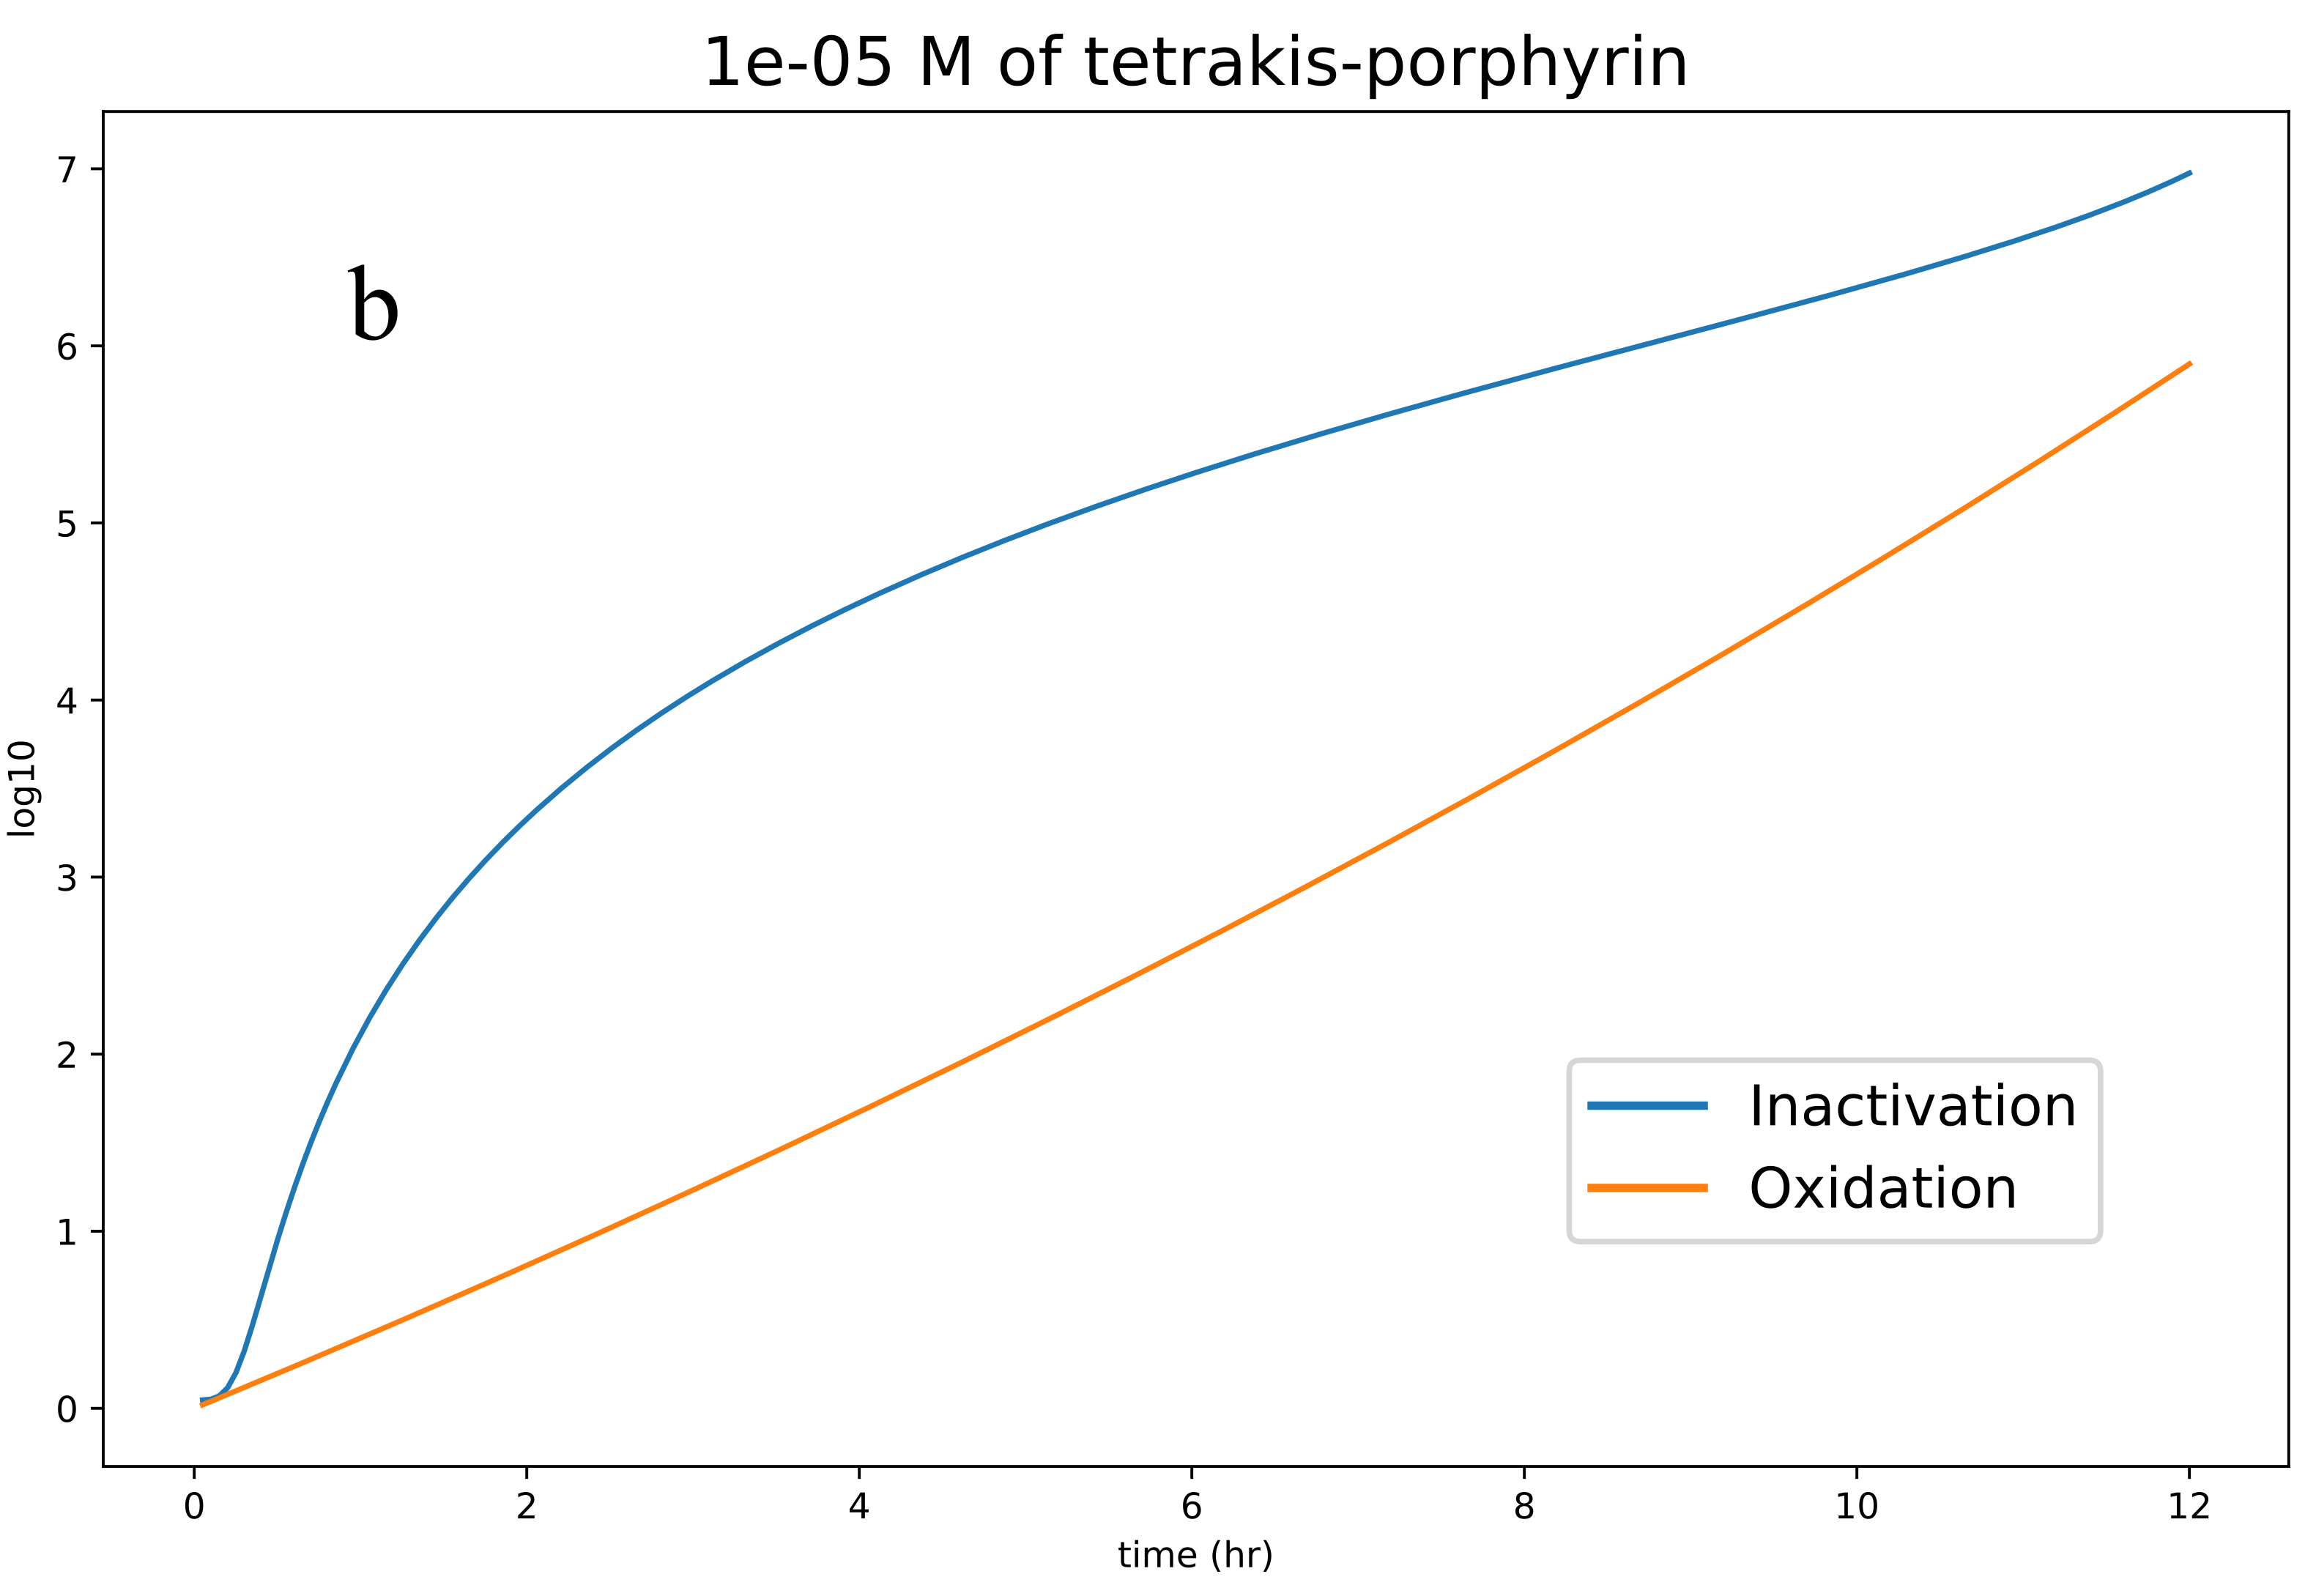
\includegraphics[width = 0.9\textwidth]{images/PDIpy/examples/10uM_biofilm.png}
    \caption{
        Two exemplary figures of PDIpy replications of the Beirao et al. data for a) planktonic and b) biofilm bacterial states.
    }
    \label{beirao_et_al}
\end{figure}

\begin{figure}
    \centering
    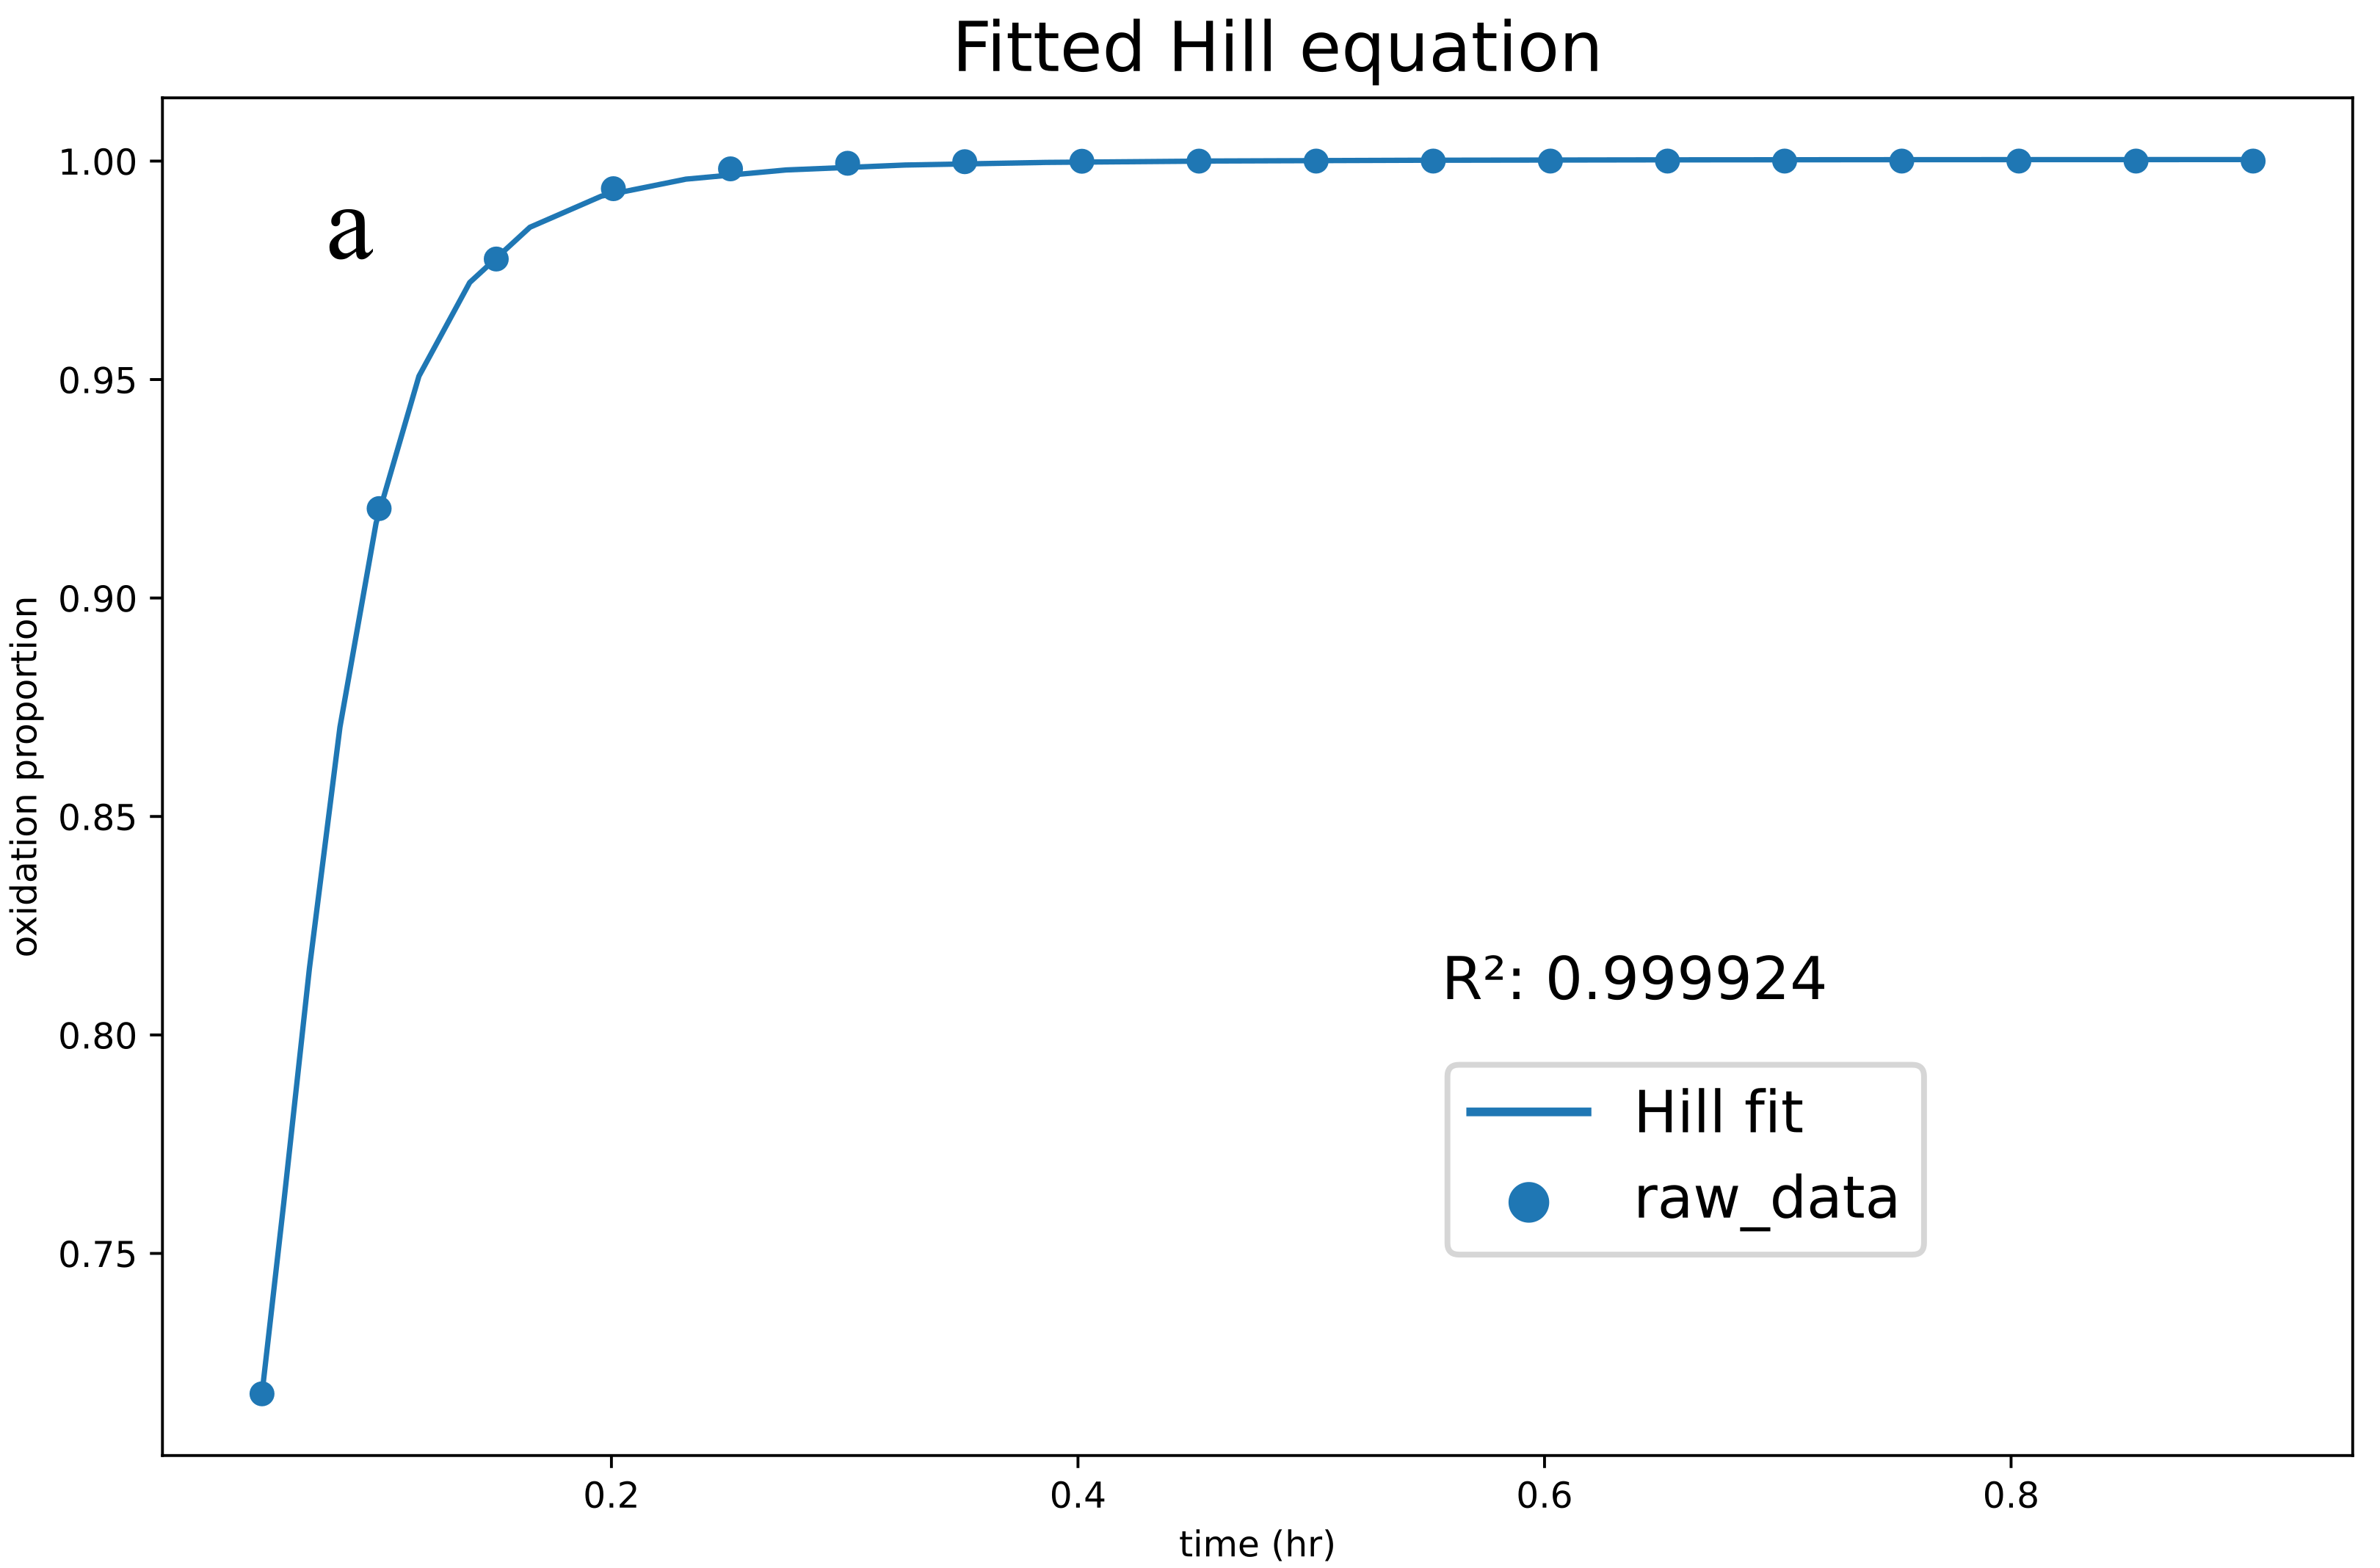
\includegraphics[width = 0.9\textwidth]{images/PDIpy/examples/20uM_regression.png}
    \vspace{5mm}
    \midrule
    \vspace{5mm}
    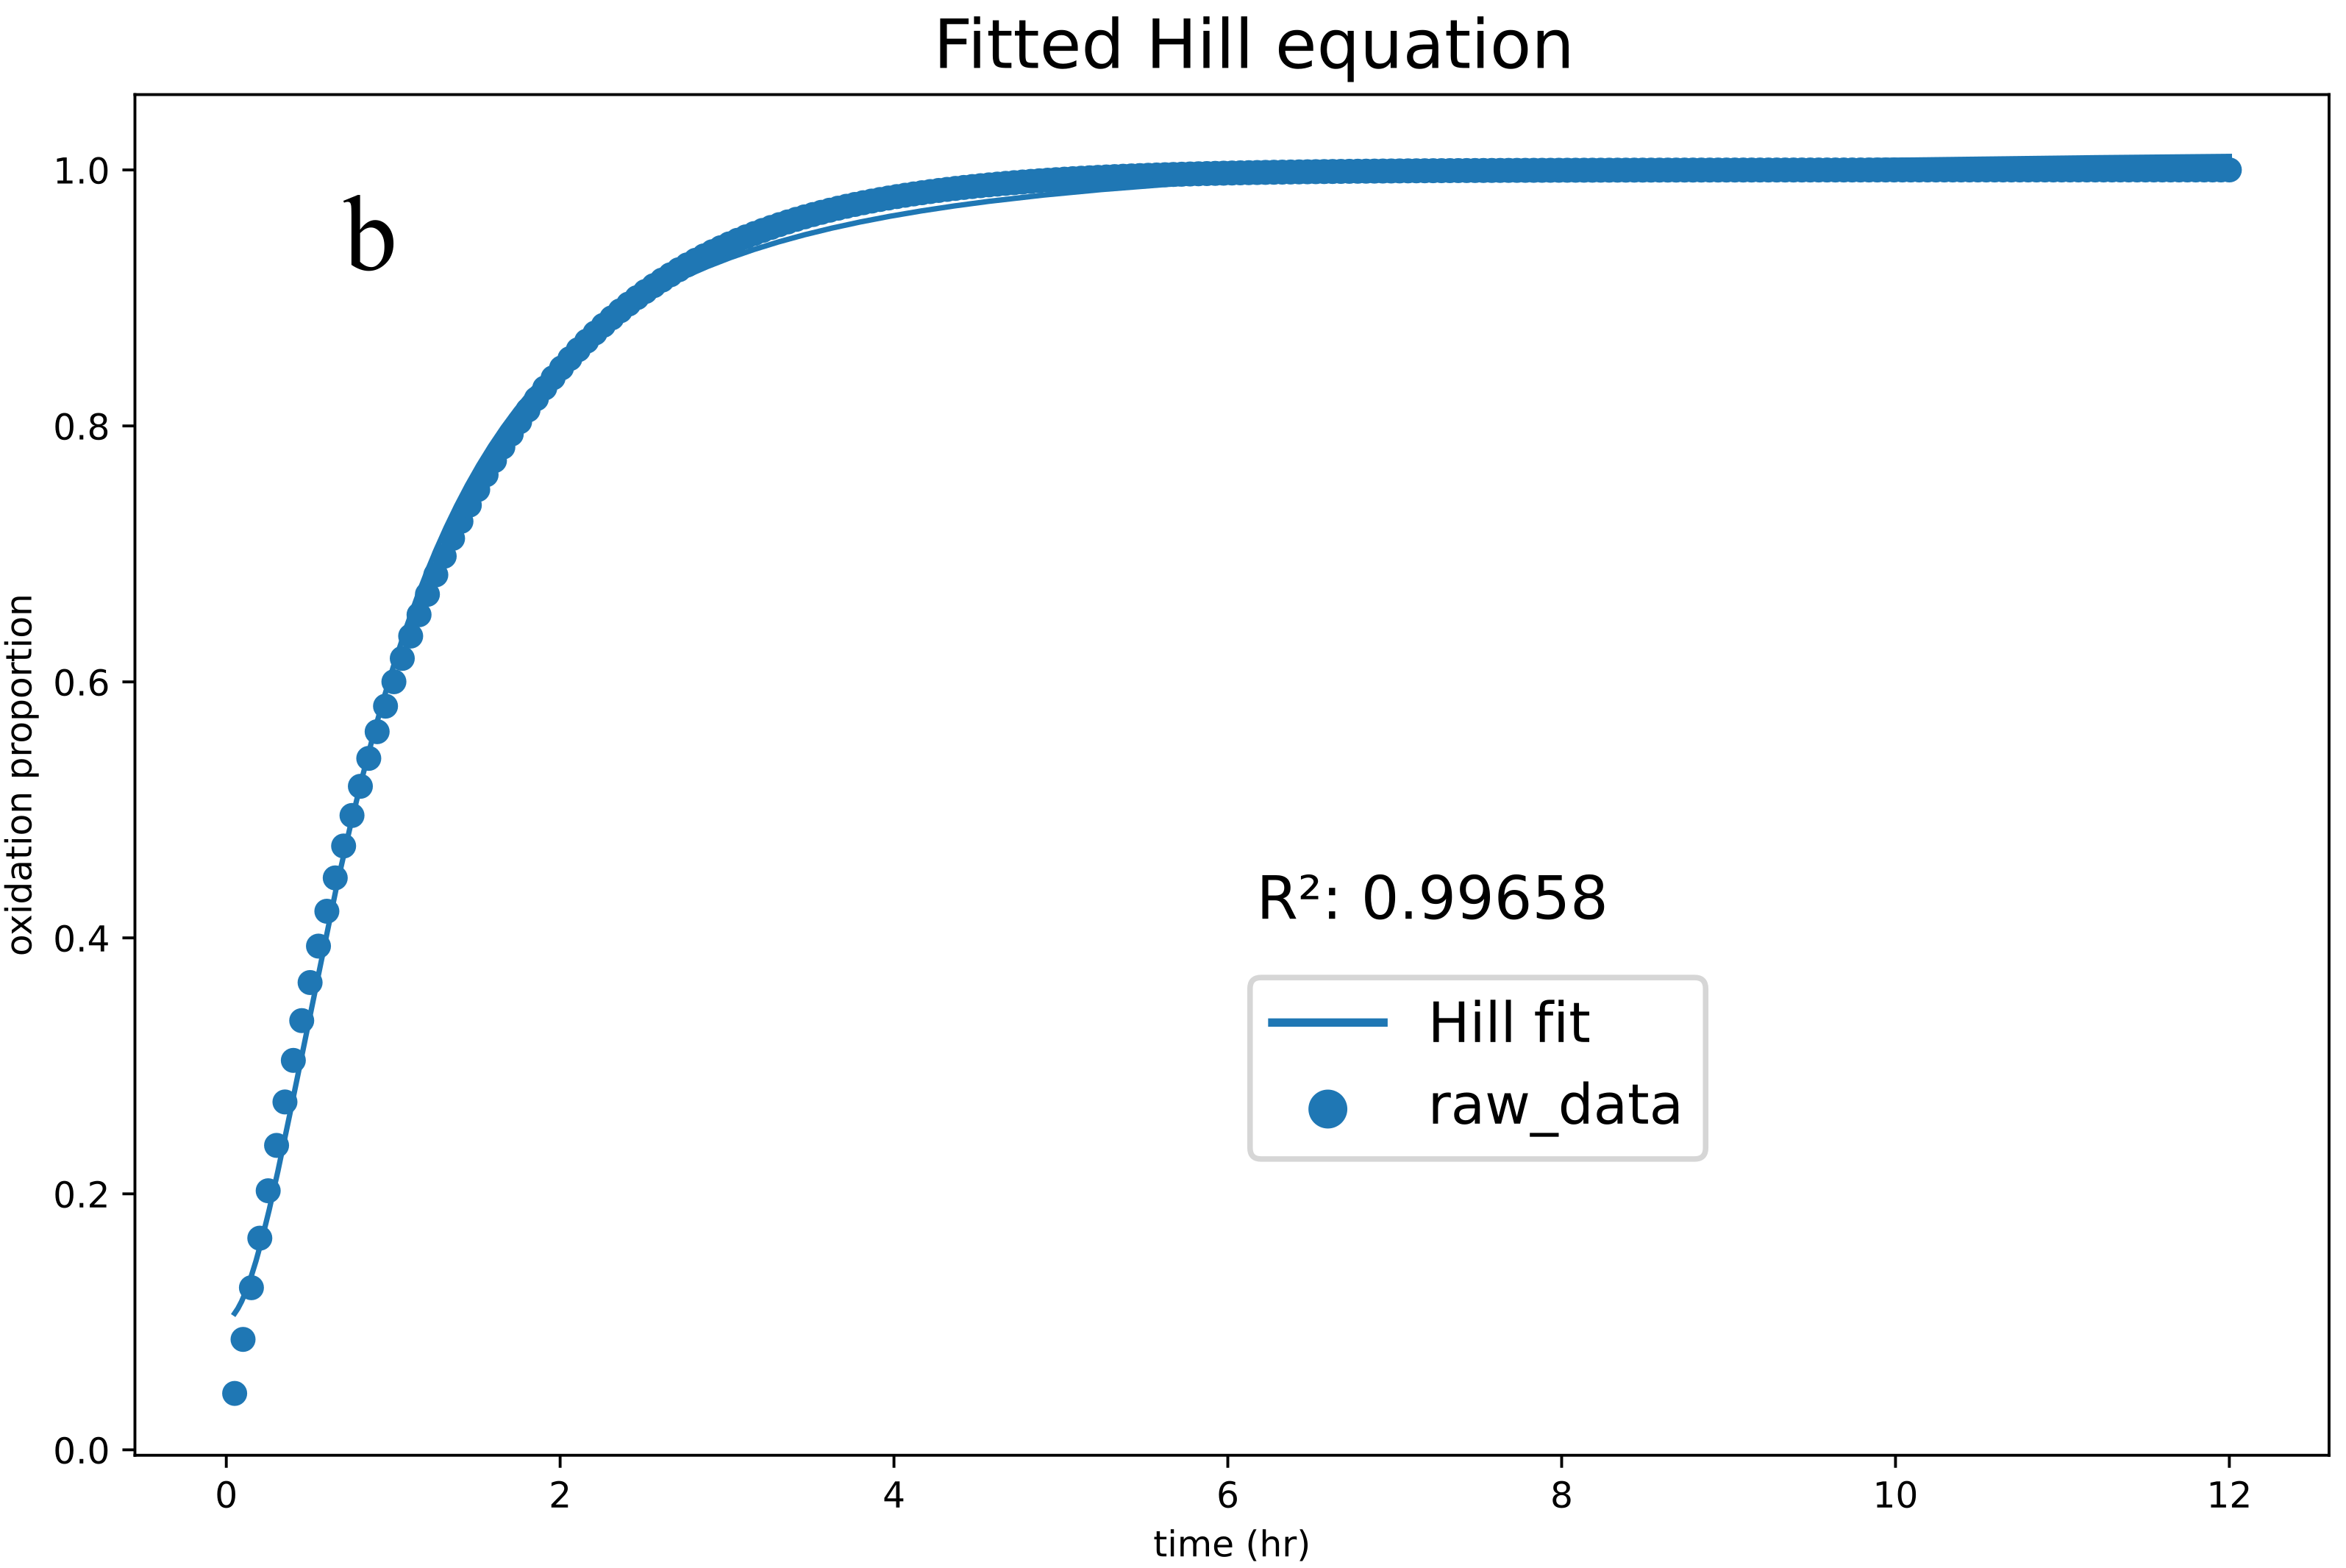
\includegraphics[width = 0.9\textwidth]{images/PDIpy/examples/10uM_biofilm_regression.png}
    \caption{
        The Hill-equation regression of the oxidation plot from Figure \ref{beirao_et_al}a. The high $R^2$ correlation supports that our chemical model of PDI is a sensible recreation of the fundamental biochemistry.
    }
    \label{hill_regression}
\end{figure}


\section{Sensitivity analyses}

\paragraph{Light intensity}
The sensitivity of simulation results to light intensities, across the range of $[10, 100,000] Lux$, was explored. The trend over this 3-log range, which is represented by Figure \ref{light_intensities}, is that the proportion of excited PS asymptotically approches 100\%. The influence of photobleaching appears to be negligible at the examined time length and light intensity, where a negative slope in the plotted excitation proportion would be expected over time as a decreasing proportion of PSs are able to electronically excite. The analysis further clarifies the minmal value of greater irradiation beyond $\approx 13,000 lux$ from the perspective of exciting PSs, which may be an informative for experimentalists when designing PDI systems.

\begin{figure}
    \centering
    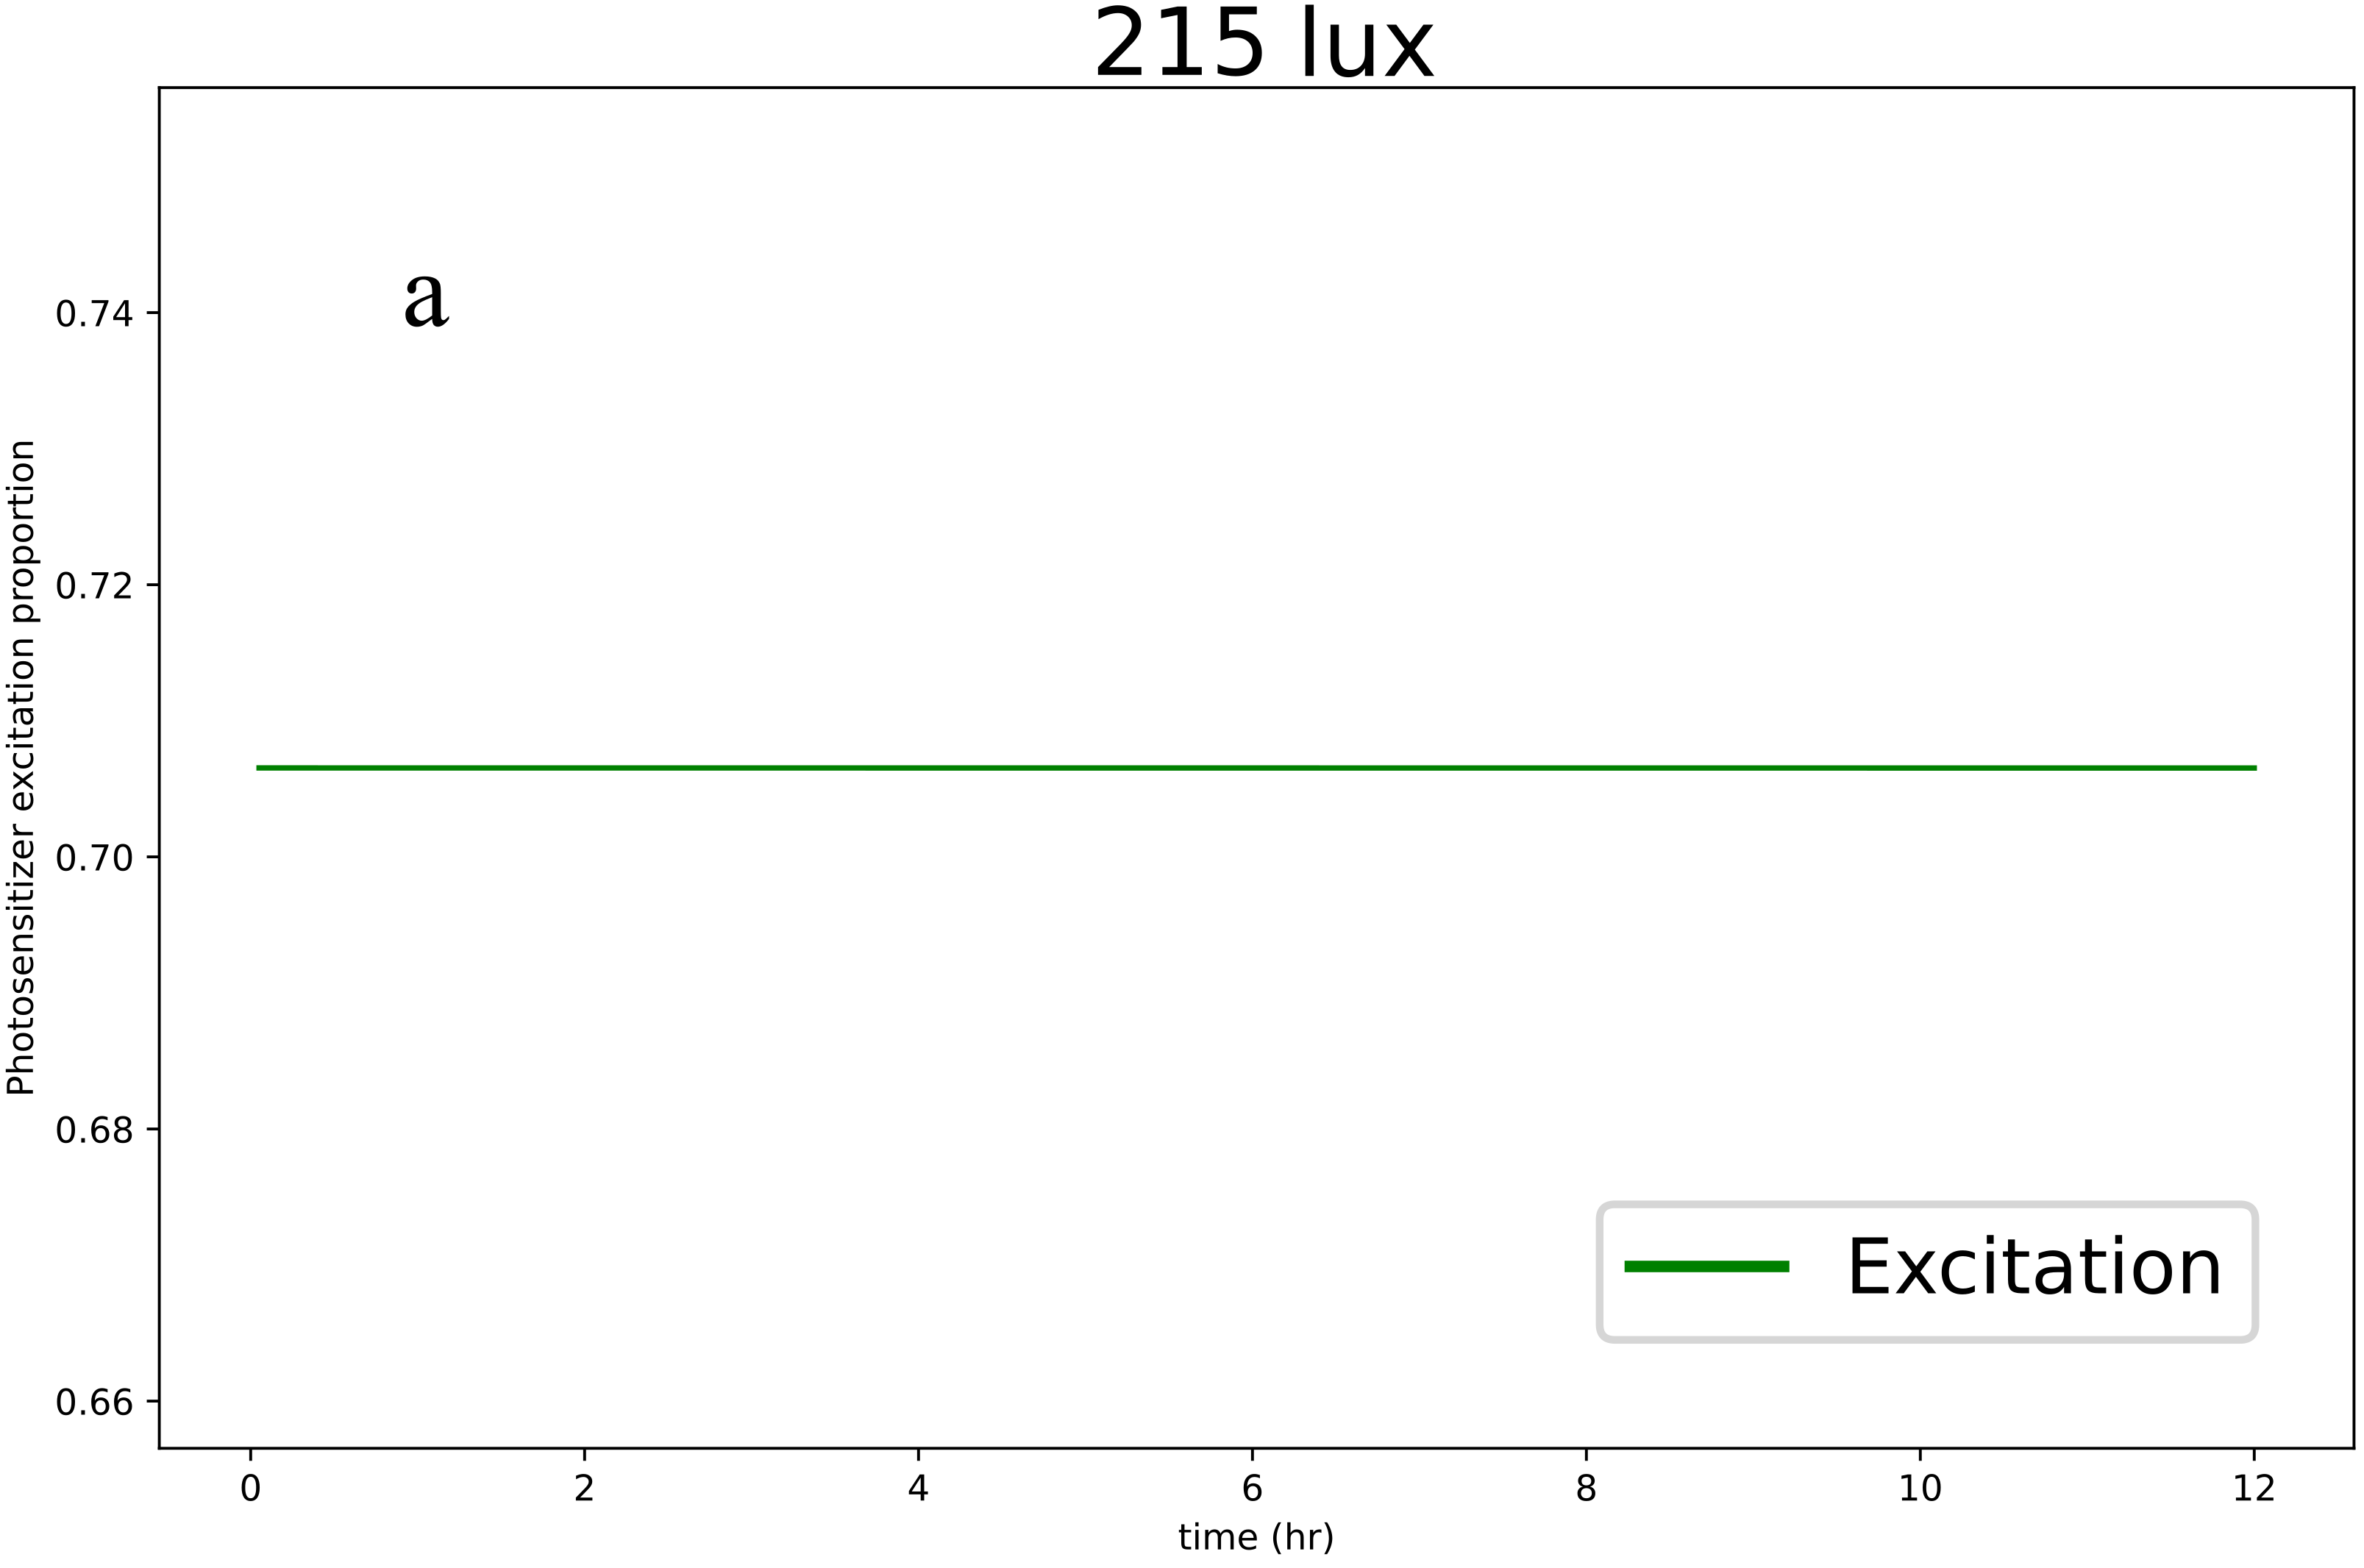
\includegraphics[width = 0.8\textwidth]{images/PDIpy/sensitivity_analyses/215_lux.png} \\
    \vspace{5mm}
    \midrule
    \vspace{5mm}
    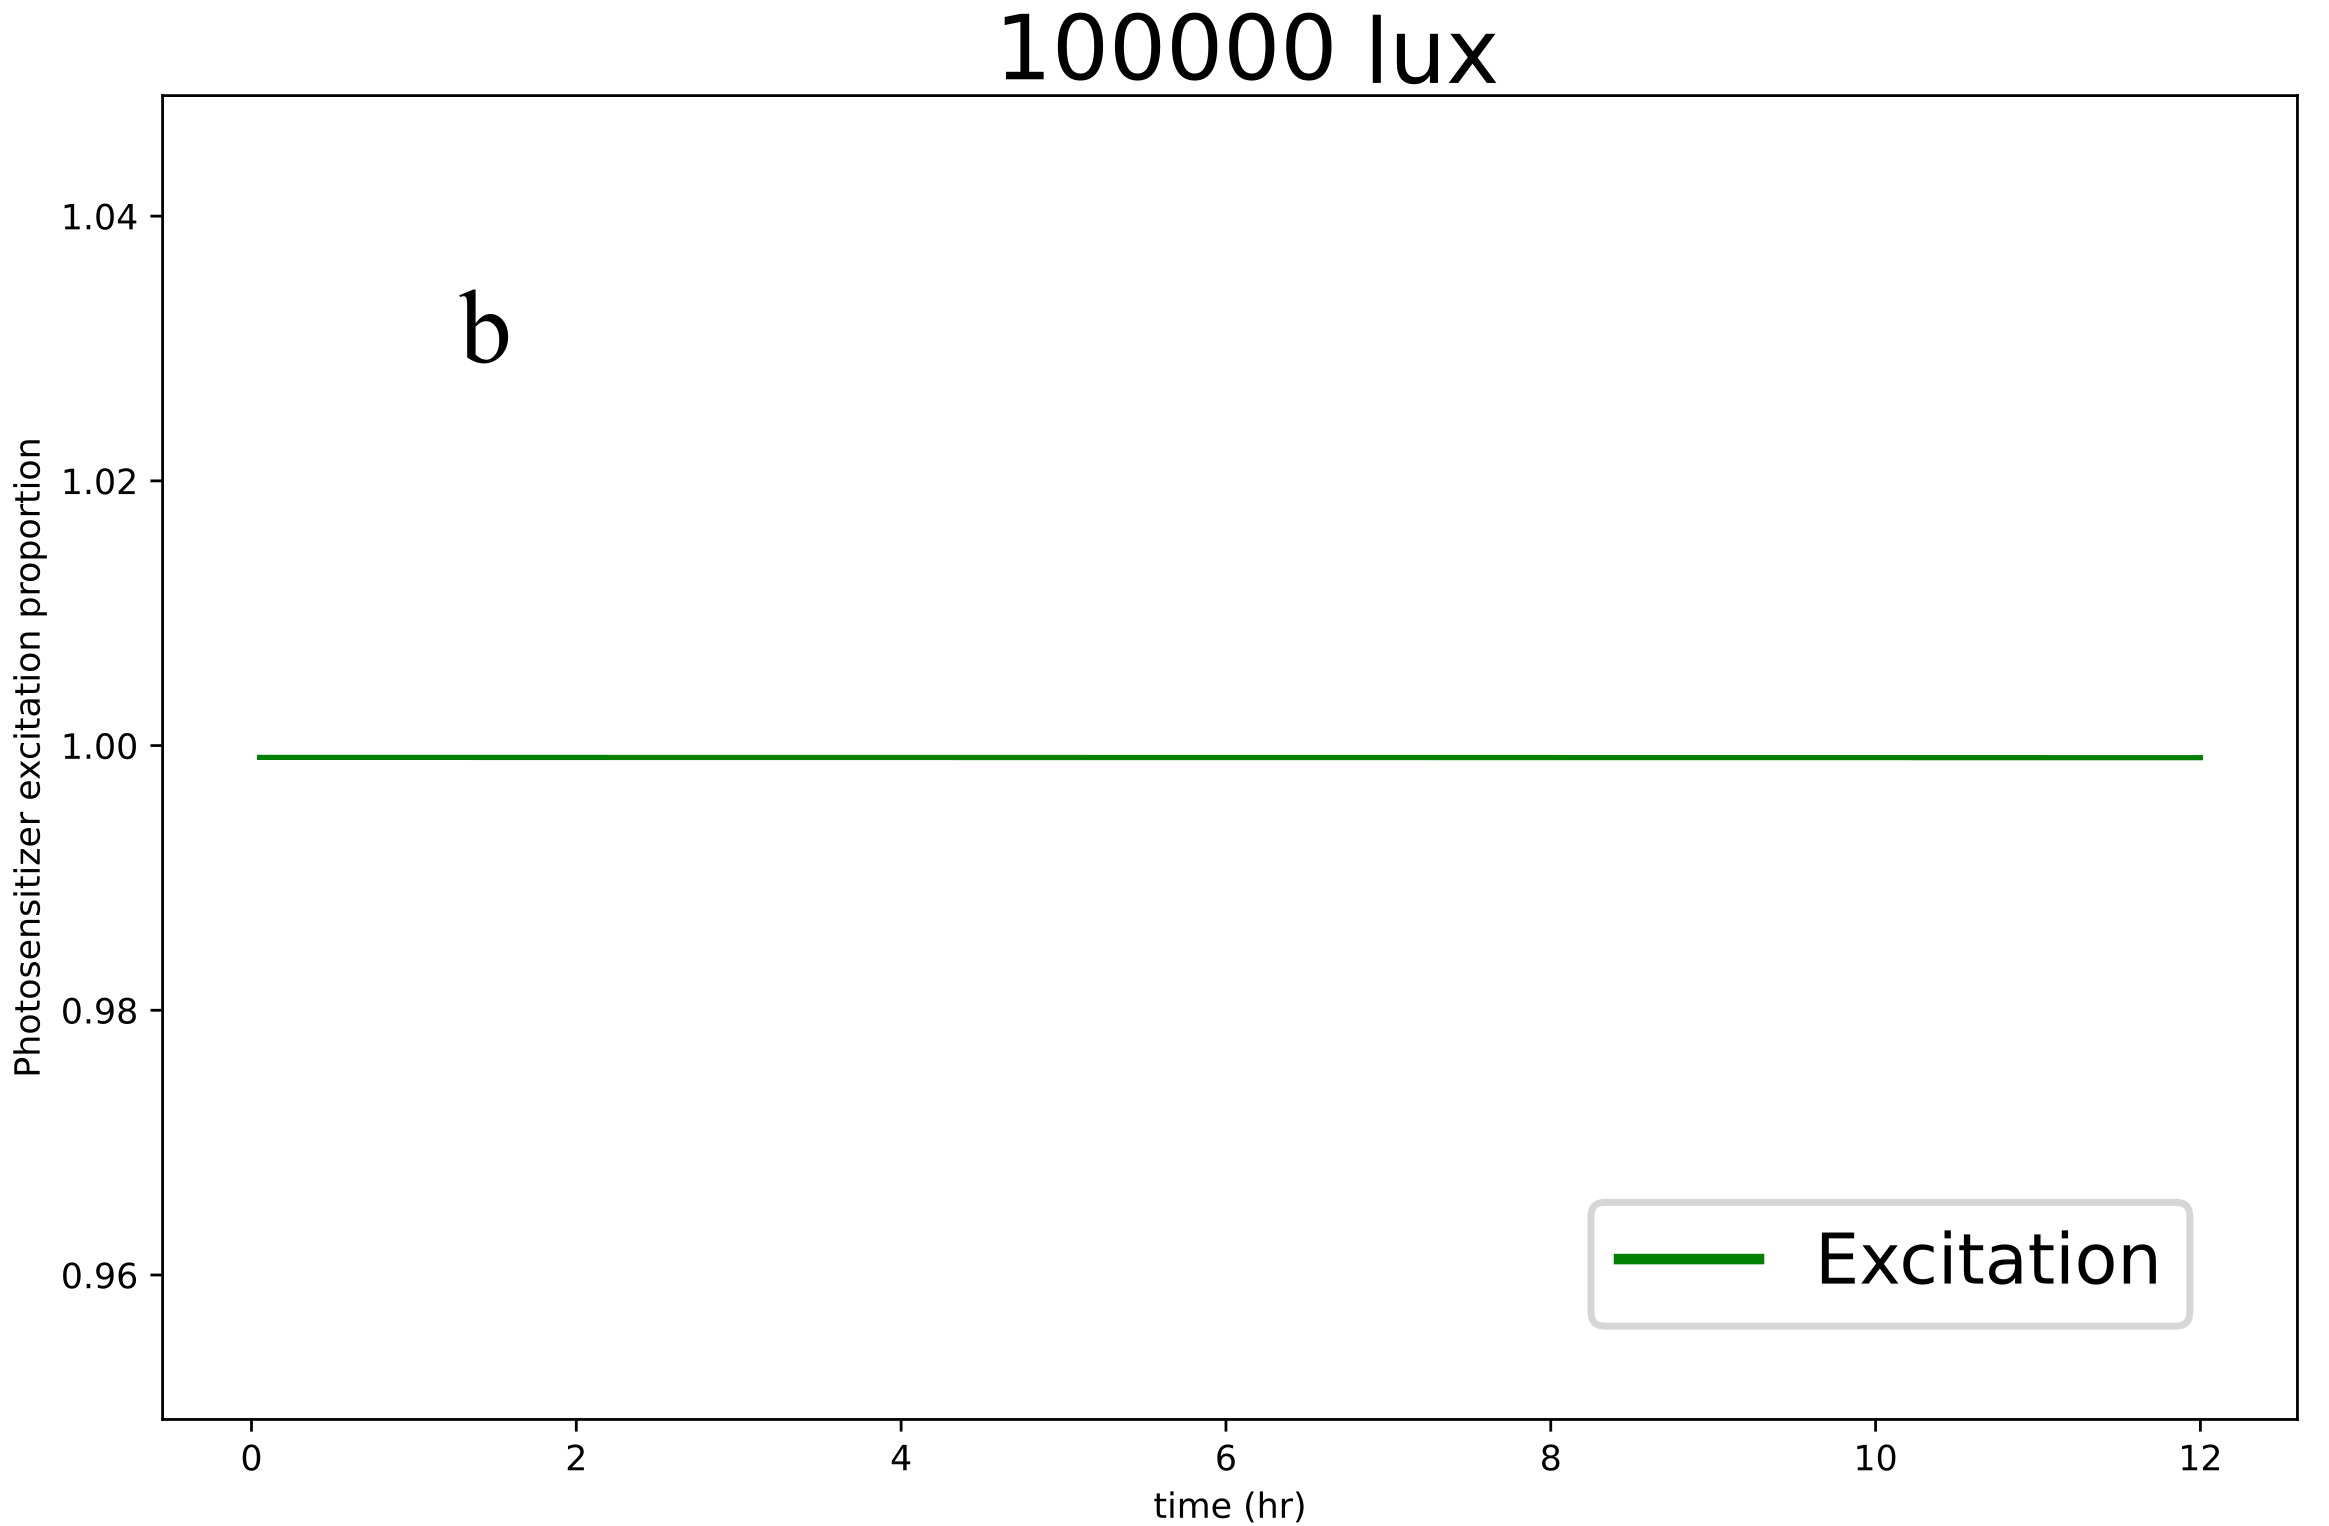
\includegraphics[width = 0.8\textwidth]{images/PDIpy/sensitivity_analyses/100000_lux.png}
    \caption{
        The proportion of excited PS at two contrasting light intensities: a) $215 Lux$ and b) $100000 Lux$. The negative slope of the plots is the consequence of photobleaching, where the quantity of excitable PSs decreases over time. This effect is more prominent in b) since the light intensity is much greater than a), and since photobleaching is a function of light intensity.
    }
    \label{light_intensities}
\end{figure}

\section{Discussion}
The preliminary examples of PDIpy with the study from Beirao et al. support that the underlying kinetic model sufficiently represents PDI. The excessive breadth in the simulation predictions, where the log-inactivation predictions with low concentrations occurs too late while the log-inactivation predictions with high concentrations occurs too early, may be resolved with adjusted the Hill parameters that are defined in Table \ref{hill_parameters}. The tighter spread of the biofilm simulation relative to the planktonic simulation supports this method of improving the predicted results, where the different set of parameter adjustments may be better tailored to inactivation phenomena. 

The sensitivity analysis of the light intensity revealed that the relationship between the proportion of PS excitation and the light intensity plateaus beyond $\approx 10,000 lux$. This insight and this type of broad inquiry over a range of values cannot be replicated with existing PDI models, since they neither consider the fundamental kinetics that results in PS excitation nor are encapsulated in a dynamic interface like the PDIpy API.  

The open-source implementation of this model in PDIpy will practically support experimentalists as they develop PDI technologies, and will ideally inspire other computational biologists to develop programs that can foster discovery of antibiotic methods at an imperative time to prevent antimicrobial resistant epedemics.   


\section{Author Contributions}
\begin{description}
    \item[APF] Designed, executed, and codified the project.
    \item[JRK] Guidance and manuscript edits.
    \item[HLB] Guidance, manuscript edits, and funding.
\end{description}

\section{Acknowledgments}

The authors are grateful to Ethan Sean Chan for his development of the framework for iPDIpy, which will be introduced in a future release of PDIpy. The authors thank the members of the Buckley and Wolff Groups at the University of Victoria for contributing ideas and data that were used to refine this PDI model. Andrew finally thanks Hiroaki Imoto for his contributions and guidance in developing the HillFit module that was used to fit data in PDIpy.
\newpage
\subsection{Supporting Information: PDIpy}

\subsection{Molecular properties and mechanisms}
The electronic difference between $^1\Delta_g$ and $^3\Sigma_g^-$ is best depicted through their respective molecular orbital diagrams in Figure \ref{mo_diagrams}. The photochemical processes of $^1\Delta_g$ generation are depicted in Figure \ref{jablonski_diagram}, while the subsequent oxidation reactions are sampled in Figure \ref{schenck_mechanism}.

\begin{figure}
    \centering
    \begin{tabular}{c|c}
        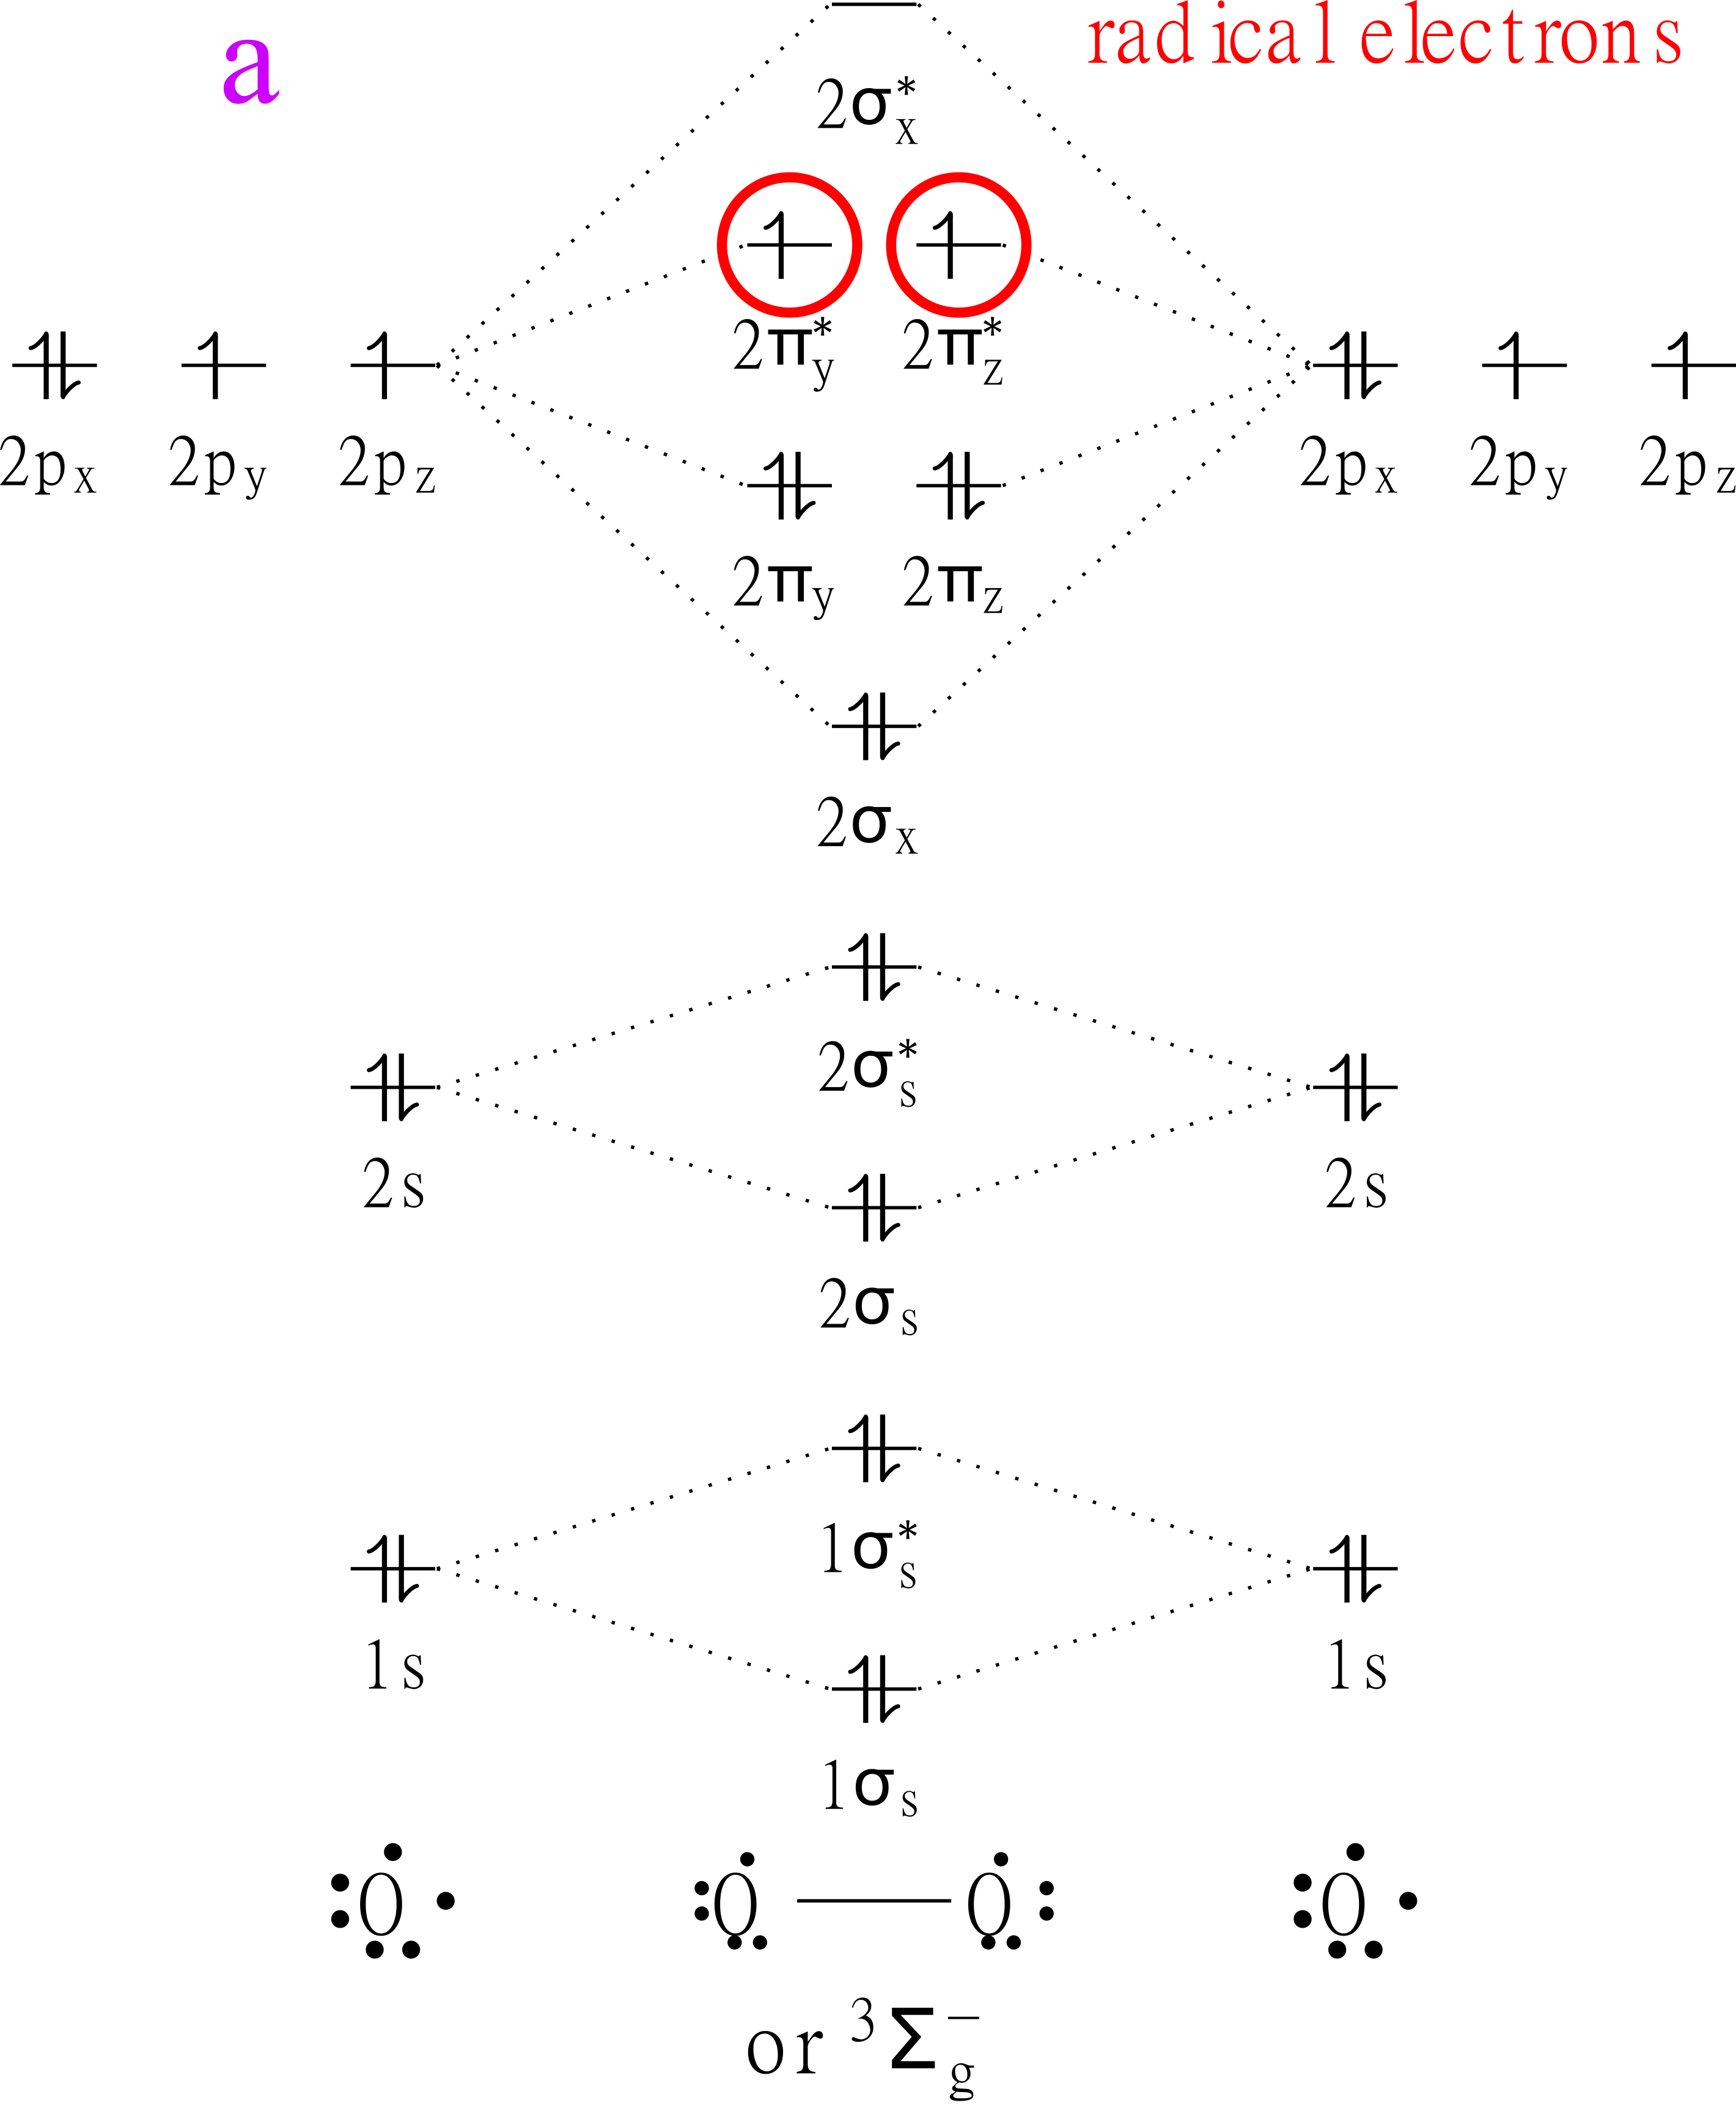
\includegraphics[width = 0.48\textwidth]{images/PDIpy/background/triplet_mo_diagram.png}
        & 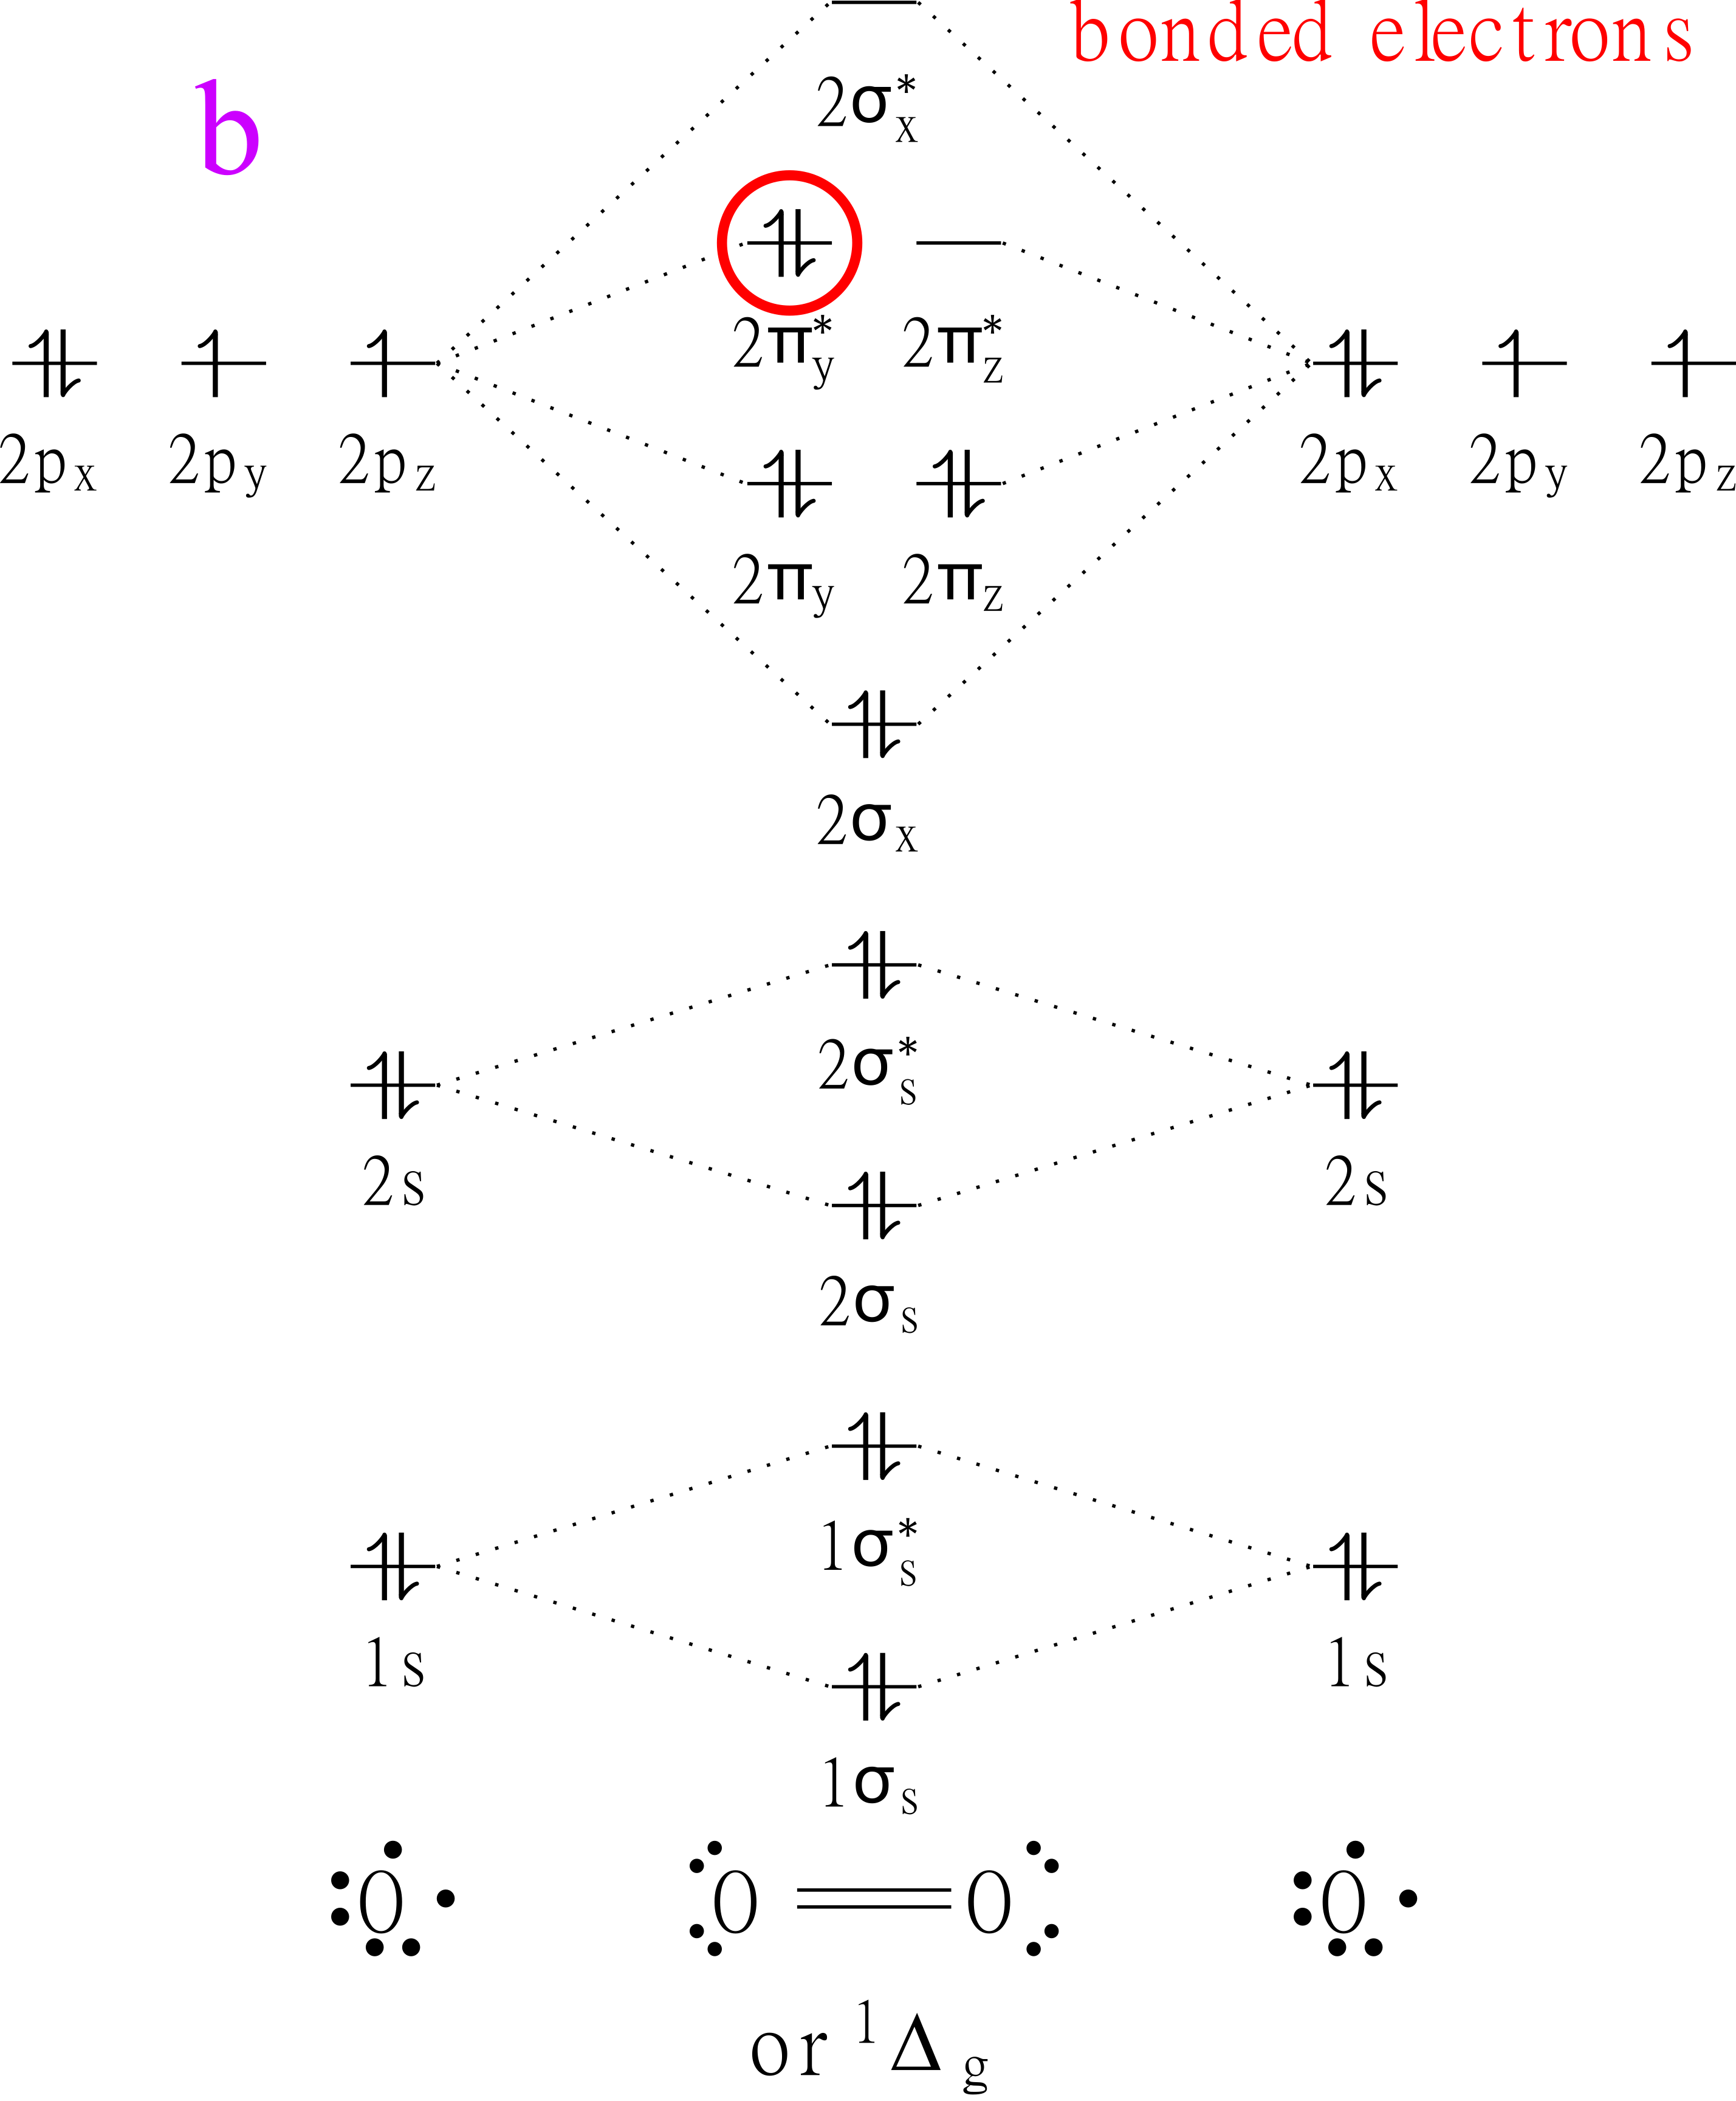
\includegraphics[width = 0.48\textwidth]{images/PDIpy/background/singlet_mo_diagram.png}
    \end{tabular}
    \caption{
        Qualitative orbital diagrams for a) $^3\Sigma_g^-$ and b) $^1\Delta_g$ configurations of diatomic oxygen. Each barbed arrow represents a single electron, and each platform represents the electronic sub-orbital of the respective label, where orbital energy increases vertically in the diagram. The distinction between a) and b) is highlighted by the red circled electrons and labels, where $^1\Delta_g$ possesses an anti-bonding $\pi^*$-bond in its HOMO that destabilizes it relative to $^3\Sigma_g^-$.
    }
    \label{mo_diagrams}
\end{figure}

\begin{figure}[t]
    \centering
    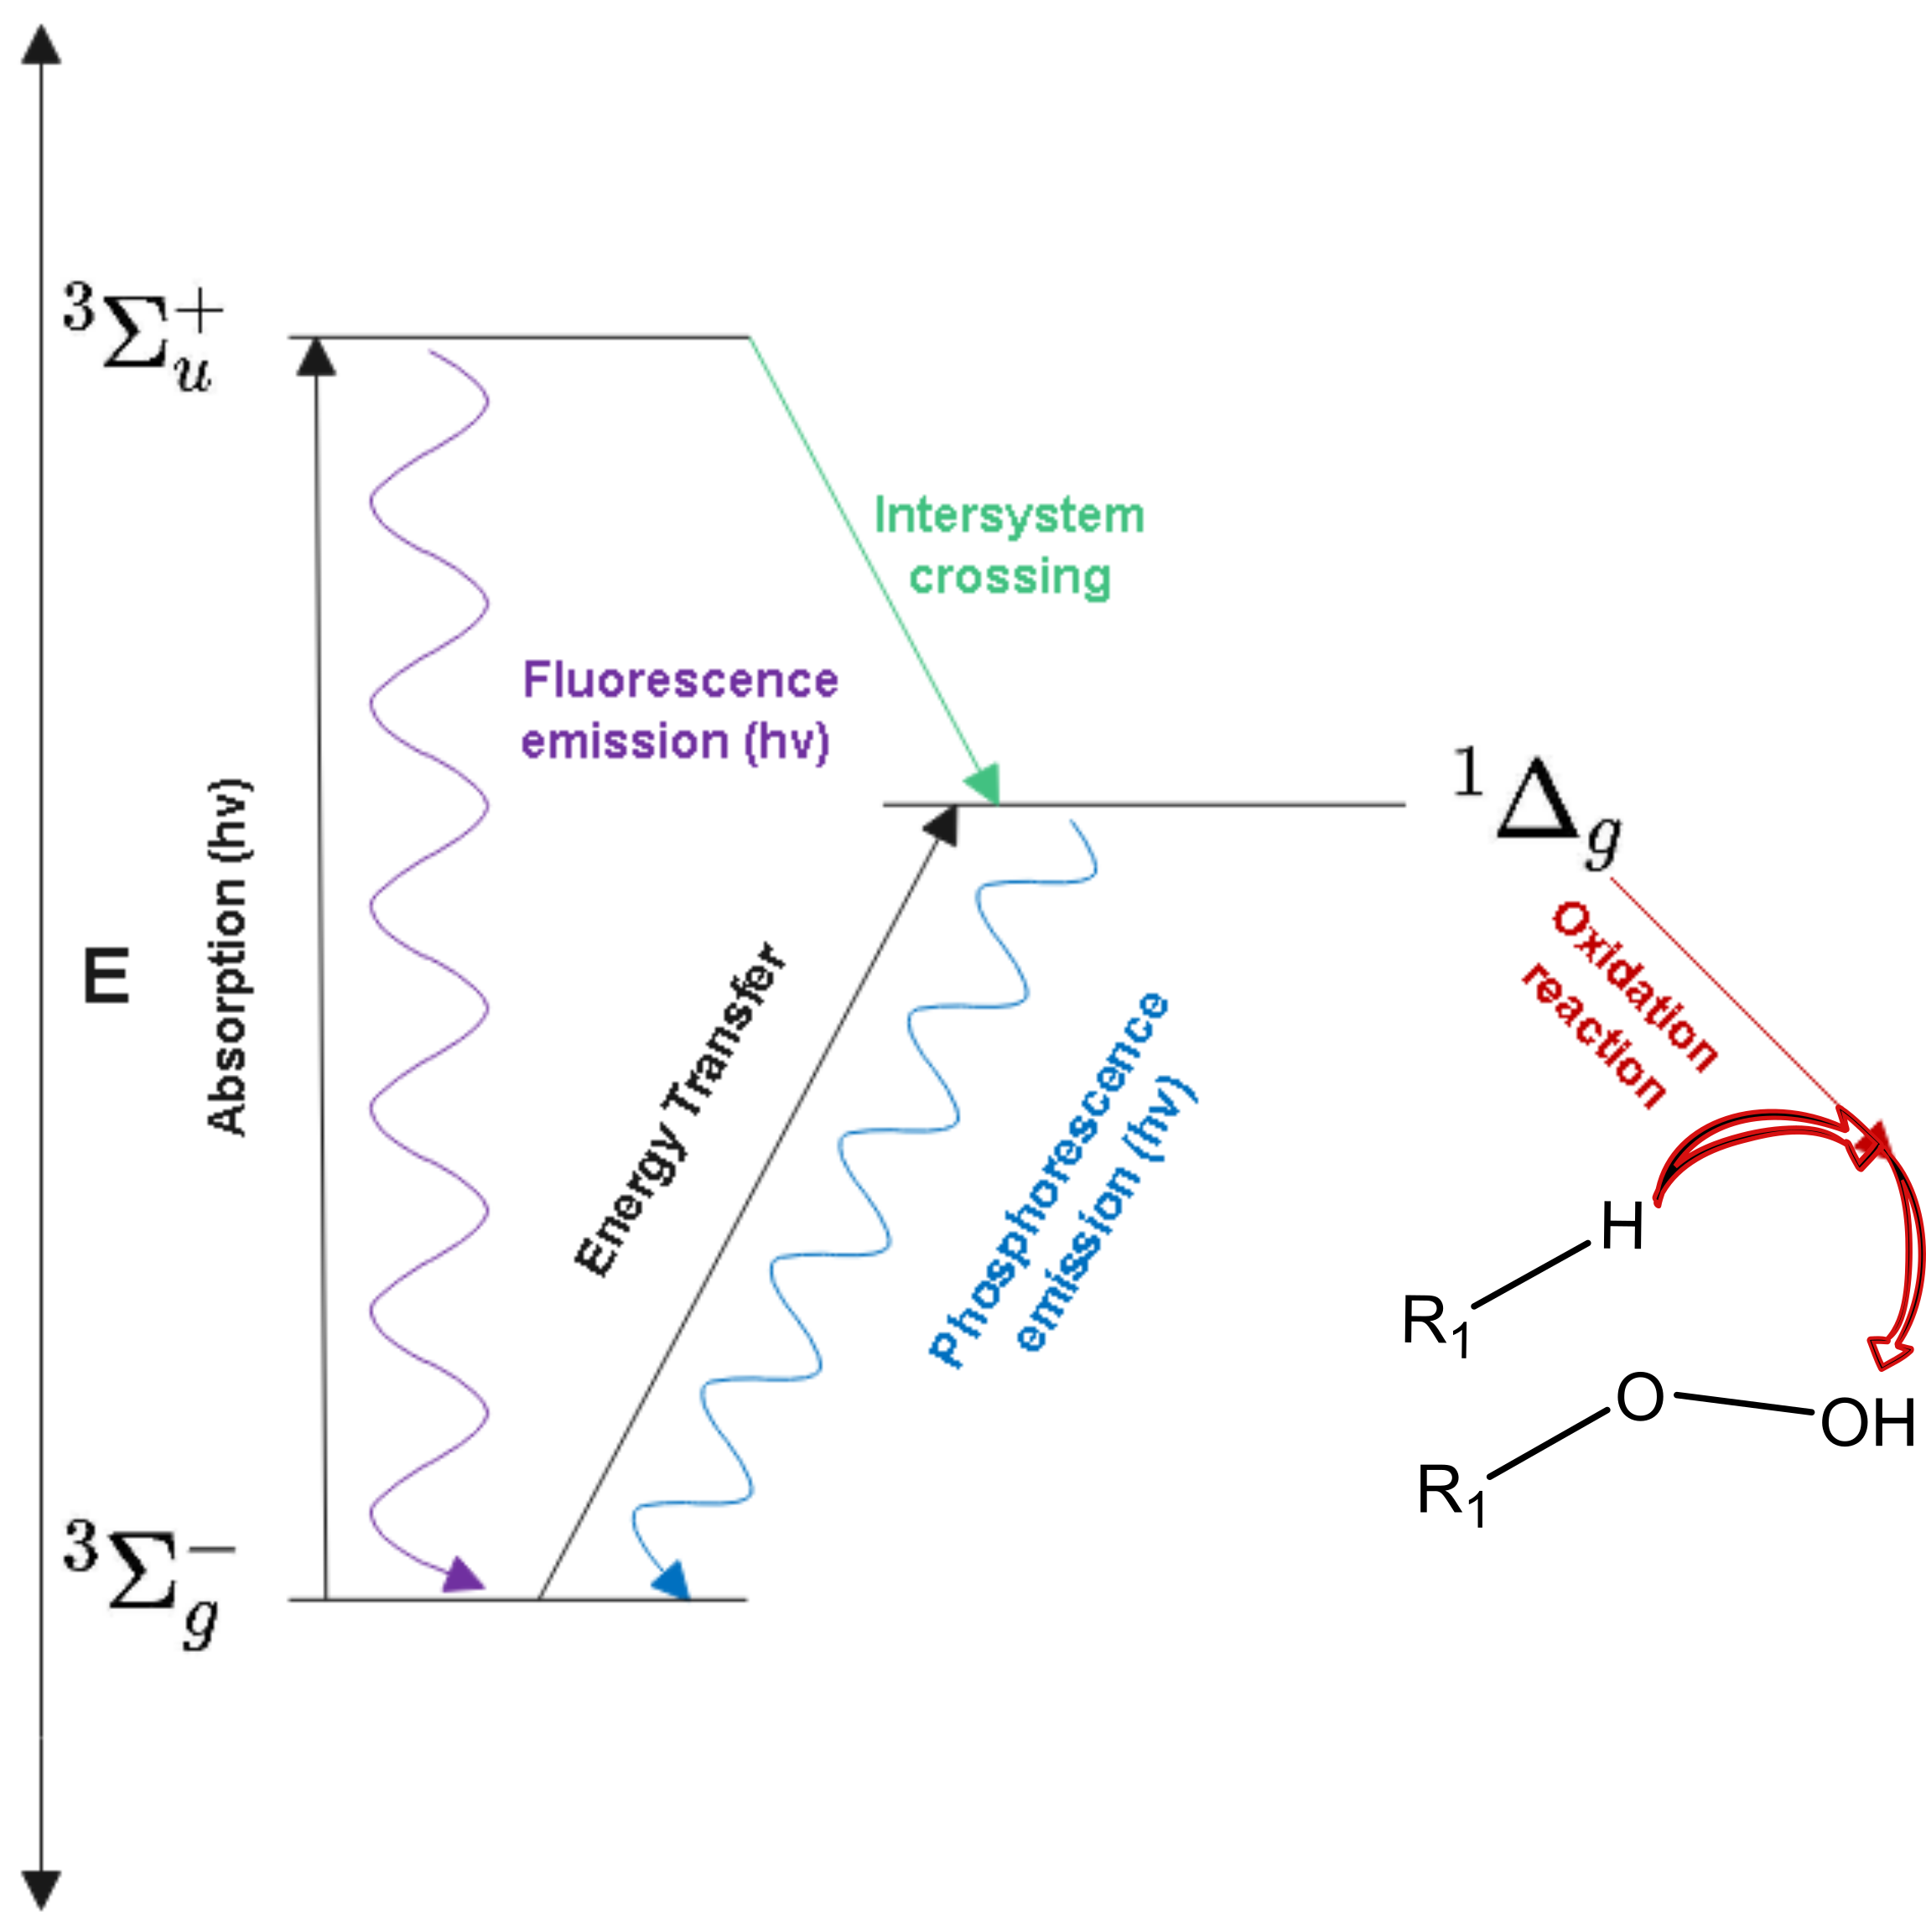
\includegraphics[width = \textwidth]{images/PDIpy/background/jablonski_diagram.png}
    \caption{
        A qualitative Jablonski energy diagram of Steps b-c of PDI. The initial excitation in PDI occurs via an energy transfer $\ce{^3\Sigma_g^- ->[energy transfer] ^1\Delta_g}$. The ROS then, while abstaining from phosphoresce, oxidizes a biological substrate to form a peroxide that gradually compounds to cause lysis.
    }
    \label{jablonski_diagram}
\end{figure}

\begin{figure}[t]
    \centering
    \includegraphics[width = \textwidth]{images/PDIpy/background/BCFA_schenck_oxidation_2.png}
    \caption{
         The reaction mechanisms of Type II oxidation and subsequent decompositions. \textbf{Step (1)} depicts the concerted \cite{Foote1968PhotosensitizedOxygen} Schenck reaction. \textbf{Step (2)} depicts the homolytic cleavage of the hydroperoxide bond to form $\ce{OH^.}$ and an oxy radical that may enter autoxidation (Type I oxidation) mechanisms. \textbf{Step (3)} depicts radical propagation via hydrogen abstraction to form another radical substrate and an alcohol byproduct. \textbf{Step (4)} is a concerted Russell reaction \cite{Russell1957Deuterium-isotopeRadicals,Howard1968TheMechanism} between two peroxides that forms a $\ce{H2O2}$, an $\alpha,\beta$-ketone, and an alcohol. The reactions of Steps (2-4) sample the wide range of possible decompositions that follow oxidation mechanisms.
    }
    \label{schenck_mechanism}
\end{figure}

\subsection{Excitation proportion} \label{excitation_proportion_estimate}

The steps for estimating the absorbed proportion of incident photons by photosensitizers, where absorbance or transmittance measurements are not available, are detailed through the following steps. a) The reported intensity of incident light from the respective light source -- i.e. irradiance ($\frac{mW}{cm^2}$), lux ($\frac{lumen}{m^2}$), or lumens (lumens) -- is converted into a quantity of incident watts $watts_{in}$ ($\frac{J}{s}$). b) This incident wattage is attenuated by the proportion of the emission spectra $spec_{em}$ that resides within the $spec_{ex}$ of the PS, 
\begin{equation}
    watt_{ex} = \frac{spec_{ex}}{spec_{em}}*watts_{in}.
\end{equation}
c) The $watt_{ex}$ is then used to calculate the moles of incident photons that strike photosensitizers per timestep 
\begin{multline} \label{photons_per_second}
    \frac{photons_{strike~PS}}{timestep}=\frac{<h\nu_{ex}>}{h*c}*watts_{ex} *\frac{s}{\Delta t}*reflection*scattering*\frac{1~mole}{N_A}*\frac{vol_{PS}}{vol_{total}},
\end{multline}
where $reflection \approx 96 \%$ and represents the proportion of incident photons that penetrate an aqueous solution \cite{Gross1993SingletLiposomes}; and $scattering \left(\frac{I_z}{I_0} = e^{-k*z}\right)$ represents the proportion of light $\frac{I_z}{I_0}$ that reaches a specified depth $z$ \cite{RobertW.1973TheSea}, where $k$ is the attenuation coefficient that is $\approx 0.04~(\frac{1}{m})$ \cite{Lorenzen1972ExtinctionPhytoplankton} for clear water. The quotient $\frac{vol_{PS}}{vol_{total}}$ describes the fraction of the solution volume where the PS resides ($vol_{total}$) that is comprised of the PS per se ($vol_{PS}$), which is calculated as the product of the quantity of PS molecules and the volume per molecule according to its molecular structure. The average excitation wavelength of the PS ($<h\nu_{excitation}>$) is calculated as the weighted average of the Soret and Q excitation bands, in proportion to their relative contribution in generating $^1\Delta_g$ \cite{Nitzan2001PhotoinactivationWavelengths,Hoenes2020PhotoinactivationWavelength}, which assumes that both excitation wavelengths are excited during the simulation. The resultant $\frac{photons_{strike~PS}}{timestep}$ from \cref{photons_per_second} is then divided by the quantity of photons that enter the system per timestep $\frac{photons_{total}}{timestep}$ to determine which fraction of photons strike a photosensitizer. 

\subsection{Deduction of inactivation via the Hill equation}

Inactivation may alternatively be deduced from oxidation through parameter manuipulation of a fitted sigmoidal curve, similar to other models \cite{Xiong1999AInactivation}. The Hill-equation \cite{Gesztelyi2012ThePharmacology} is a sigmoidal model that derives from mass-action kinetics, similar to the Michaelis-Menten kinetic model, and thus it was selected the signmoidal model for this alternative framework. A Python program for fitting the Hill-equation was developed -- the HillFit module -- with a variation of the Hill-equation \cite{Inoue2016OscillationActivation} 
\begin{equation} \label{hill_eq}
    y=bottom+\frac{(top-bottom)*x^n}{EC50^n+x^n},
\end{equation}
that introduces an additional $bottom$ parameter for more advantageous fitting. The predicted oxidation data was fitted to a hill-equation via HillFit and the parameters were subsequently adjusted in Table \ref{hill_parameters} to optimally meet the training data. The $top$ parameter of \cref{hill_eq} is adjusted asymptotically to a limit that follows an subtly different empirical expression for planktonic $1-10^{-\Omega}$ than biofilm $1-10^{-0.7-\Omega }$ simulations, where $\Omega = wattage^{\frac{1}{5}}-log10(1-final_{oxidation\_proportion})$. This limit manifests in the predicted inactivation being $\approx [1,2]-log$ greater than the predicted oxidation, which implicitly specifies an oxidation thereshold of $\approx [1,10]\%$. The different parameter adjustments between sessile and planktonic systems may be explained that numerous chemical influences, such as diffusion rates, are not explicitly considered in our kinetic model. The regression plots for the fit of the Beirao et al. training data is depicted in Figure \ref{hill_regression}. The very precise fitting -- $R^2 > 0.996$ -- supports that the Hill-equation is an accurate description of our kinetic PDI model, and conversely that our model fundamentally describes a biochemical relationship.

\begin{figure}
    \centering
    \includegraphics[width = 0.9\textwidth]{images/PDIpy/training/10uM_regression.png}
    \vspace{5mm}
    \midrule
    \vspace{5mm}
    \includegraphics[width = 0.9\textwidth]{images/PDIpy/training/10uM_biofilm_regression.png}
    \caption{
        The Hill-equation regressions for the oxidation plots of the Beirao et al. training data for a) planktonic and b) sessile states. The high $R^2$ correlation supports that our chemical model of PDI recreates a sigmoidal biochemical relationship. The greater number of data points in panel b) is the consequence of a far longer simulation time than the simulation of panel a).
    }
    \label{hill_regression}
\end{figure}

% \begin{table}
%     \centering
%     \begin{tabular}{l|c|c}
%         \textbf{Bacterial state} & \textbf{Hill parameter} & \textbf{Adjustment} \\
%         \multirow{2}{}{Planktonic} & EC50 & -76\% \\
%          & nH & +100\% \\
%     \end{tabular}
%     \caption{
%         The Hill parameters adjustments that are enacted to create the inactivation plot for simulations of planktonic systems. 
%     }
%     \label{hill_parameters}
% \end{table}

\subsection{Oxidized membrane region}
The region of the bacterial membrane that is oxidized by cross-linked PSs may be a small fraction of the total membrane, provided that the bacterium does not have a tremendous angular momentum. This is not presently captured by our model, but the following logic could incorporate this concept into the model. The oxidized region of a coccus bacterial cell can be determined from the cellular radius and volume
\begin{equation}
    radius_{cell} = \sqrt[3]{3*\frac{volume_{cell}}{4\pi}}~.
\end{equation}
The membrane volume is calculated
\begin{equation}
    volume_{membrane} = \frac{4\pi}{3}*(radius_{cell}^3 - (radius_{cell}-th_{membrane})^3)
\end{equation}
there the thickness of the cytoplasmic membrane $\approx 4 nm$. The volume of oxidized membrane is then calculated
\begin{equation}
    volume_{oxidized} = volume_{membrane}*\frac{angle_{oxidized}}{360}~,    
\end{equation}
where the $angle_{oxidized}$ describes the angle in degrees from vertical at which the farthest $^1\Delta_g$ reaches the mebrane. The fraction of the membrane volume that is oxidized is then calculated 
\begin{equation}
    oxidized = \frac{volume_{oxidized}}{volume_{membrane}} 
\end{equation}
and applied to augment the effective oxidation proportion
\begin{equation}
    oxidation_{proportion,new} = \frac{oxidation_{proportion,old}}{oxidized}~.
\end{equation}

\subsection{Sensitivity analyses}

\paragraph{Light source \& emission}
The sensitivity of simulation results to the light source -- incandescent, LED, or fluorescent -- was explored. The comparison of incandescent and LED light sources, where LED and fluorescent were nearly indistinguishable, is depicted in Figure \ref{light_source}. These simulated differences are solely attributed to differences in the proportion of emitted photons that are within the visible spectrum, since PDIpy does not current resolve the intensity of specific emitted wavelengths or consider the inactivation effects of heat from incandescent bulbs. The visible proportion of the emitted wavelengths was determined in Figure \ref{light_emission} to have minimally consequence above 20\%.

\begin{figure}
    \centering
    \includegraphics[width = 0.9\textwidth]{images/PDIpy/sensitivity_analyses/light_source/incandescent.png} \\
    \vspace{5mm}
    \midrule
    \vspace{5mm}
    \includegraphics[width = 0.9\textwidth]{images/PDIpy/sensitivity_analyses/light_source/LED.png}
    \caption{
        A comparison of the same experiment under a) incandescent and b) LED light sources. The discrepancy between the inactivation of the two sources is attributed to the proportion of emission that resides in the visible spectrum.
    }
    \label{light_source}
\end{figure}

\begin{figure}
    \centering
    \includegraphics[width = 0.9\textwidth]{images/PDIpy/sensitivity_analyses/light_emission/20_visible.png} \\
    \vspace{5mm}
    \midrule
    \vspace{5mm}
    \includegraphics[width = 0.9\textwidth]{images/PDIpy/sensitivity_analyses/light_emission/100_visible.png}
    \caption{
        A comparison of the same experiment with a light source that possesses a) 20\% visible light and b) 100\% visible light, where the former value appears -- for these simulation conditions -- to be the threshold beyond which the proportion of visible light does not substantial effect inactivation rates. This threshold is likely dependent upon the quantity of incident watts; in which case, this threshold is not broadly generaliazable for all simulation conditions.
    }
    \label{light_emission}
\end{figure}

\paragraph{Bacterial CFU/mL}
The influence of bacterial $\frac{CFU}{mL}$ upon the rate of oxidation in PDIpy was tuned to yield the trend that is depicted in Figure \ref{bacterial_cfus}, where the rate of oxidation is inversely proportional with the $\frac{CFU}{mL}$. This is intuitive, where larger bacterial populations requires more time to eradicate.

\begin{figure}
    \centering
    \includegraphics[width = 0.9\textwidth]{images/PDIpy/sensitivity_analyses/bacterial_cfus/6-log_cfu.png} \\
    \vspace{5mm}
    \midrule
    \vspace{5mm}
    \includegraphics[width = 0.9\textwidth]{images/PDIpy/sensitivity_analyses/bacterial_cfus/10-log_cfu.png}
    \caption{
        A comparison of oxidation and inactivation between a) 1E6 and b) 1E10 $\frac{CFU}{mL}$. The imposed trend is that oxidation and thus inactivation are inversely proportional to the colony size, which is the intuitive result.
    }
    \label{bacterial_cfus}
\end{figure}

\paragraph{Photobleaching constant}
The influence of photobleaching constant was explored over an 8-log range of values, which is depicted in Figure \ref{photosensitizing_constant}. The values below $1E4$ are indistinguishable over time. 

\begin{figure}
    \centering
    \includegraphics[width = 0.9\textwidth]{images/PDIpy/sensitivity_analyses/photobleaching_constant/1E4.png} \\
    \vspace{5mm}
    \midrule
    \vspace{5mm}
    \includegraphics[width = 0.9\textwidth]{images/PDIpy/sensitivity_analyses/photobleaching_constant/1E3.png}
    \caption{
        A comparison of the excitation proportion with two photobleaching constants. Constant values below 1E4 are approximately indistinguishable.
    }
    \label{photosensitizing_constant}
\end{figure}


\subsection{Supplementary figures}
This section includes supplementary figures for the main text. The natural and synthetic porphyrins that inspire the design of photosensitizers are depicted in Figure \ref{zinc_porphyrin}. 

\begin{figure}
    \centering
    \includegraphics[width = \textwidth]{images/PDIpy/background/chlorophyll.png} \\
    \midrule
    \includegraphics[width = 0.5\textwidth]{images/PDIpy/background/zinc_porphyrin.png}
    \caption{
        The chemical structure of porphyrinoid chlorophyll (top) juxtaposed with the core motif of a synthetic porphyrin analogue (bottom). The "R" groups of the synthetic porphyrin can be substituted with a range of functionality to tailor the PS for the specific PDI system.
    }
    \label{zinc_porphyrin}
\end{figure}

\newpage
\startchapter{Future work}

\section{ROSSpy}
The remaining tasks for the advancement of ROSSpy towards publishing in \textit{Desalination} are detailed in the following list:
\subsection{Necessary}
\begin{enumerate}
    \item \textbf{v0.1.0} - polish the source code and elevate the version number to $0.1.0$.
    \item \textbf{Publish} - refine the manuscript and submit it for peer-review.
\end{enumerate}

\subsection{Auxiliary}
\begin{enumerate}
    \item \textbf{Dual domain} - discern that ability to simulate reactive transport as a dual domain through PHREEQC.
    \item \textbf{Perspective} - permit users to customize the range of module distance and time that are graphed in the simulation.
    \item \textbf{iROSSpy} - embed the PHREEQC batch software with the iROSSpy script to create an operational command-line version of ROSSpy for non-technical users of the script.
    \item \textbf{evaporation} - investigate why precipitation predictions from desalination simulations quantitatively exceeded those from evaporation simulations by 50\%, despite controlling for the differences in pore volume of the solutions and the total active area of the desalination module.
\end{enumerate}

\section{PDIpy}
The remaining tasks for the advancement of PDIpy towards publishing in the \textit{BioPhysical Journal} are detailed in the following list:
\subsection{Necessary}
\begin{enumerate}
    \item \textbf{Replication} - introduce a kinetic reaction that represents bacterial replication, which may occur in the first-order in $\ce{^3O2}$ and possess a rate constant as the inverse of the doubling time in standard media conditions. This assumes that the simulated environment provides an optimum environment for bacterial growth, where experimental conditions usually provide these conditions for adequate growth, and it assumes that the examined organism metabolizes through cellular respiration, which is true for most prokaryotes that would be studied via PDI.
    \item \textbf{Absorption} - implement an optional argument for a measured absorptivity of the simulated PS solution that can complement the volume proportion approach that is currently used.
    \item \textbf{Quantum yields} - permit the disaggregation of a total $\ce{^1O2}$ quantum yield into the excitation quantum yield and the energy transfer quantum yield that are used in PDIpy, to lend flexibility to values that are available to the user.
    \item \textbf{Publish} - Refine the manuscript and submit it for peer-review.
\end{enumerate}

\subsection{Auxiliary}
\begin{enumerate}
    \item \textbf{Lysis Threshold} - discover literature that can explicitly validate the assumption that $[1,10]\%$ of a cytoplasmic membrane must oxidize before it lyzes.
    \item \textbf{iPDIpy} - connect the PDIpy script with the GUI framework that has been designed to provide an interative interface for non-technical users of PDIpy.
\end{enumerate}

\section{WCMpy}
The WCMpy suite of packages will continue to be improved with features towards publishing in the \textit{BioPhysical Journal}, such as following proposed expansions:
\subsection{Necessary}
\begin{enumerate}
    \item \textbf{Codons: tables} - expand the accepted variations of codon translations for other organisms, possibly by using the "codons-usage-table" Python module.
    \item \textbf{dFBApy: conditions selection} - add the ability to only use the kinetic data that most matches the specified conditions of temperature or pH.
    \item \textbf{dFBApy: discontinuous concentration changes} - the discrete behavior from the dFBApy example must be investigated to ensure that the counter-intuitive plots are not the result of an bug.
    \item \textbf{BiGG\_SABIO: multiple entries} - allow the refined kinetics file to provide multiple entries of data for each reaction/enzyme, which will permit the above aspiration for expanding the dFBA function.
    \item \textbf{BiGG\_SABIO: chemical synonyms} - improve the ability to match chemical and enzyme names between the BiGG and SABIO conventions.
    \item \textbf{WCMpy: cytoplasm chemistry} - amalgamate the suite of packages into an operational cytoplasmic model.
    \item \textbf{WCMpy: visualization} - visualize geometric growth of a cell over the simulation.
    \item \textbf{WCMpy: biofilms} - apply a WCMpy model to a biofilm community, within the framework of the CA algorithm.
    \item \textbf{WCMpy: Publish} - update the manuscript, with the above changes, and submit it for peer-review.
\end{enumerate}

\subsection{Auxiliary}
\begin{enumerate}
    \item \textbf{Codons: protein analysis} - visualize and interpret translated proteins through the "Minotaor" Python module.
    \item \textbf{Codons: GC~\%} - calculate the fraction of a genome that consists of Guanine and Cytosine, which is an influential property for biophysical experiments.
    \item \textbf{Codons: back translation} - determine the potential genetic sequences that beget a known protein sequence, expanding upon the "backtranslate" Python module.
    \item \textbf{BiGG\_SABIO: real-time analysis} - assess the alignment of the scraped SABIO-RK reaction data to the GEM reaction as the data is acquired, where only matched data is retained. This will importantly prevent the scraped file from bloating to $\approx 4 GB$ for full-scale GEMs, albeit at the expense of slightly longer computational time.
\end{enumerate}


% \bibliography{references.bib}
\printbibliography %[keyword=major,heading=subbibliography,title={Major Sources}]
% \printbibliography[keyword=minor,heading=subbibliography,title={Minor Sources}]

\end{document}
